\documentclass[11pt,a4paper]{book}
\usepackage[francais]{babel}
\usepackage[utf8]{inputenc}
\usepackage{amsmath,amssymb,amsthm}
\usepackage{mathrsfs,stmaryrd}
\usepackage{fancybox,mdframed,multicol,comment,datetime}
\usepackage{framed} % pour encadrer
\usepackage[dvipsnames]{xcolor}

\usepackage{fourier}
\usepackage{imakeidx}% imakeidx ne met pas les liens?
\usepackage[backref]{hyperref}
\hypersetup{
    colorlinks=true,       % false: boxed links; true: colored links
    linkcolor=[rgb]{0,0.2,0.6},          % color of internal links
    citecolor=[rgb]{0,0.2,0.6},        % color of links to bibliography
    filecolor=[rgb]{0,0.2,0.6},      % color of file links
    urlcolor=[rgb]{0.7,0.2,0.2}           % color of external links
}

\usepackage[all]{hypcap} % règle pb cible des liens hyperref
\usepackage{pgf,pgfmath,tikz}
\usetikzlibrary{arrows}
\usetikzlibrary[patterns]
\tikzset{every picture/.style={execute at begin picture={
   \shorthandoff{:;!?};}
}}

\usepackage[margin=2.5cm]{geometry}

\usepackage[normalem]{ulem} % pour souligner avec changements de ligne
\usepackage{esvect} % pour jolis vecteurs avec \vv

\everymath{\displaystyle} 



\theoremstyle{definition}
\newtheorem{theoreme}{Théorème}[chapter]
\newtheorem{definition}[theoreme]{Définition}
\newtheorem{lemme}[theoreme]{Lemme}
\newtheorem{proposition}[theoreme]{Proposition}
\newtheorem{corollaire}[theoreme]{Corollaire}
\newtheorem{remarque}[theoreme]{Remarque}
\newtheorem{ex}{Exercice}


\newcommand{\N}{\mathbb N}
\newcommand{\Z}{\mathbb Z}
\newcommand{\Q}{\mathbb Q}
\newcommand{\R}{\mathbb R}
\newcommand{\C}{\mathbb C}
\newcommand{\U}{\mathbb U}
\newcommand{\F}{\mathbb F}


%%%%%%%%%%%%%%%%%%%%%%%%%%%%%%%%%
%%%%%% MISE EN FORME CLUB %%%%%%%
%%%%%%%%%%%%%%%%%%%%%%%%%%%%%%%%%

%\pagestyle{empty}



% En-tête des feuilles :

\newcommand{\enTete}[1]{
\noindent \textbf{\textsf{\href{http://depmath-nancy.univ-lorraine.fr/club/}{Club Mathématique de Nancy} \hfill Institut Élie Cartan}}
\hrule
\begin{center}
{\Huge \textbf{#1}}
\end{center}
\hrule
\vspace{1em}
}


%----- Structure des exercices ------

\newenvironment{prerequis}{(\bfseries Prérequis:}{)\newline}


% commenter une des deux lignes suivantes suivantes suivant l'option choisie:


% - - - - - - - - - - - - - -
% PARAMETRAGE DU PACKAGE ANSWERS 
% POUR LES INDICATIONS ET CORRECTIONS
% - - - - - - - - - - - - - - 

\usepackage{answers}



\Newassociation{sol}{Soln}{solutions}
% ira dans le fichier d'identifiant 'solutions'
% et écrira les solutions dans un environnement 'Soln'
\Newassociation{hint}{Hint}{indications}
\Newassociation{hint2}{Hint2}{indications2}
%\newenvironment{exo}{
%\begin{ex} \label{enonce.\theex}
%
%}
%{~\hyperref[indication.\theex]{[Indications]}
%~\hyperref[solution.\theex]{[Correction]}~\end{ex} }


\usepackage{xparse}
\NewDocumentEnvironment{exo}{o}
 {\label{enonce.\theex} \IfNoValueTF{#1}
   {\ex\addcontentsline{toc}{section}{\protect\numberline{\theex}  }}
   {\ex[#1]\addcontentsline{toc}{section}{\protect\numberline{\theex}#1}}%
   \ignorespaces}
 {~\hyperref[indication.\theex]{[Indications]}
~\hyperref[solution.\theex]{[Correction]}~\endex\medskip\hrule}
 
 


\renewenvironment{Hint}[1]{
\vspace{1em}
\noindent \textbf{Indications pour l'exercice #1} (retour à l'\hyperref[enonce.#1]{énoncé}, voir la \hyperref[solution.#1]{correction}) 
\phantomsection\label{indication.#1}
}

\renewenvironment{Hint2}[1]{
\vspace{1em}
\noindent \textbf{Deuxième indication pour l'exercice #1} (retour à l'\hyperref[enonce.#1]{énoncé}, voir la \hyperref[solution.#1]{correction}) 
\phantomsection\label{indication2.#1}
}

\renewenvironment{Soln}[1]{
\vspace{1em}
\noindent \textbf{Correction de l'exercice #1} (retour à l'\hyperref[enonce.#1]{énoncé}, retour à l'\hyperref[indication.#1]{indication}) 
\phantomsection\label{solution.#1}
}




% - - - - - - - - - - - - - - 
% FIN PARAMETRAGE ANSWERS
% - - - - - - - - - - - - - - 

%-----------------------------
% MACROS POUR LES FEUILLES DE TD



\newcommand{\debut}{
	\Opensolutionfile{indications}[\jobname_hints]
	\Opensolutionfile{indications2}[\jobname_hints2]
	\Opensolutionfile{solutions}[\jobname_sol]
	
}
\newcommand{\fin}{
	\Closesolutionfile{indications}
	\Closesolutionfile{indications2}
	\Closesolutionfile{solutions}
	\chapter{Indications pour la résolution des exercices}
	\Readsolutionfile{indications}
	\newpage
	\chapter{Indications supplémentaires}
	\Readsolutionfile{indications2}
	\newpage
	\chapter{Correction des exercices}
	\Readsolutionfile{solutions}
	%\newpage
	%\printindex
	%\indexprologue{\small Dans cet index, vous trouverez toutes les mathématiciennes et mathématiciens cités dans ce texte}
	%\printindex[p]
	
}
 % choix 1 : les corrections sont regroupées à la fin du document
%\input{macros_sans_answers} %  choix 2 : les correction suivent les énoncés

\newcommand*{\etoile}
{
\begin{center}
$\star$\par
$\star$\hspace*{3ex}$\star$
\end{center}
}

%\makeindex
%\makeindex[name=p,title=Index des mathématiciennes et mathématiciens cités,columns=3]
% et ne pas oulbier de faire un vrai "makeindex"

%\excludecomment{prerequis} % décommenter pour maxquer les prérequis

\usepackage{fontawesome}
\begin{document}
% TODO : notations
% TODO index
% TODO : biographies de matheux avec photos ?

% TODO : biblio
% TODO : notes bibliographiques / thématiques


\debut % pour le début des macros answers, si applicable


\title{Une année d'exercices au \\ Club Mathématique de Nancy\footnote{\url{depmath-nancy.univ-lorraine.fr/club}}\\ \faCogs}
\author{Clémence Karmann, Régine Marchand, Damien Mégy, Tom Riblet}
\date{Version préliminaire, compilée le \today\\ La version la plus à jour de ce document se trouve à l'adresse \url{https://github.com/dmegy/club}}
\maketitle

\begin{multicols}{2}
\tableofcontents
\end{multicols}


%%%%%%%%%%%%%%%%%%%%%%%%%%%%%
\chapter*{Présentation}
%%%%%%%%%%%%%%%%%%%%%%%%%%%%%

Document en cours de rédaction. Si vous trouvez une faute, qu'une correction ne vous semble vraiment pas claire (ou qu'elle n'est manifestement pas terminée), ou que vous avez des propositions pour améliorer quoi que ce soit, n'hésitez pas à transmettre vos remarques pendant les séances du club.


Les exercices ne correspondent pas forcément exactement à ceux des feuilles distribuées lors des séances : certains exercices ont été supprimés (trop difficiles, ou bien non traités en séance), leur ordre a parfois été modifié, des explications ont été rajoutées etc.

 
Cependant la différence avec ce qui a été distribué est minime et les feuilles originales sont accessibles sur le site du club.

%%%%%%%%%%%%%%%%%%%%%%%%%%%%%
\paragraph{Sources}
%%%%%%%%%%%%%%%%%%%%%%%%%%%%%


Les exercices présentés ici sont rarement originaux, ils ont été adaptés à partir de diverses sources : livres, sites internet (pages personnelles, sites institutionnels comme Culturemath ou Images des maths, Wikipedia, bases de données d'exercices comme exo7...).

Voir la bibliographie en fin de recueil, ainsi que les indications bibliographiques données dans les énoncés ou dans les corrections.

%%%%%%%%%%%%%%%%%%%%%%%%%%%%%
%\chapter{Notations}
%%%%%%%%%%%%%%%%%%%%%%%%%%%%%

%\paragraph{Parties entières inférieures et supérieures}
%\label{partie-entiere}
%\index{partie entière!inférieure}\index{partie entière!supérieure}

%Si $x$ est un réel, on note $\lfloor x\rfloor$ sa partie entière inférieure, c'est-à-dire l'entier relatif immédiatement inférieur (ou égal). Par exemple, $\lfloor 3\rfloor=3$, $\lfloor 3,1\rfloor=3$ et $\lfloor -3,1\rfloor=-4$.
%De même, on note $\lceil x\rceil$ sa partie entière supérieure, c'est-à-dire l'entier relatif immédiatement supérieur (ou égal). Par exemple, $\lceil 3\rceil=3$, $\lceil 3,1\rceil=4$ et $\lceil -3,1\rceil=-3$.

%\paragraph{Partie fractionnaire}



%%%%%%%%%%%%%%%%%%%%%%%%%%%%%
\chapter{Principe des tiroirs}
%%%%%%%%%%%%%%%%%%%%%%%%%%%%%


Considérons pour commencer l'exercice suivant :

\begin{exo}[Les chaussettes]
Dans son tiroir, Stanislas a des chaussettes bleues, vertes et rouges. Il fait noir. \\
Combien de chaussettes doit-il prendre dans son tiroir pour être sûr d'en avoir (au moins) deux de la même couleur ?
\end{exo}

\vspace{1em}
Cet exercice paraîtra sans doute trop évident au lecteur ou à la lectrice : il y a trois couleurs différentes pour les chaussettes. En prenant quatre chaussettes, on est assuré d'en avoir au moins deux de la même couleur.

Malgré la grande simplicité du raisonnement, de simples variantes peuvent parfois ne pas sembler aussi évidentes. Prenons par exemple la variation suivante.

%%%%%%%%%%%%%%%%%
\begin{exo}[Anniversaires]
\begin{enumerate}
\item
Le lycée Dirichlet compte $400$ élèves. Montrer qu'il existe (au moins) deux élèves qui fêtent leur anniversaire le même jour.

\item Même avec un peu moins d'élèves, on aurait pu avoir la même conclusion. Quel est le nombre minimal d'élèves à partir duquel on peut obtenir la même conclusion ?

\item À partir de combien d'élèves dans un lycée peut-on affirmer qu'il en existe  (au moins) trois avec la même date d'anniversaire ?
\end{enumerate}
\begin{sol}
\begin{enumerate}
\item
Comme il y a plus d'élèves que de jours dans l'année, il y a au moins deux élèves qui fêtent leur anniversaire le même jour.

\item À partir de $367$ élèves, on peut conclure de la même manière.

\item S'il y a $2\times 366=732$ élèves, il est possible qu'exactement deux d'entre eux fêtent leur anniversaire chaque jour. À partir de $2\times 366+1=733$ élèves, il y en a forcément trois qui fêtent leur anniversaire le même jour.
\end{enumerate}
\end{sol}
\end{exo}

\vspace{1em}
Cet exercice semble-t-il toujours aussi évident ? Il est vrai qu'on peut le résoudre de tête (la réponse se trouve en base de la page\footnote{La réponse à la dernière question est $733$. (Oublier l'existence des années bissextiles conduit à la réponse $731$.)}), mais il faut savoir qu'il existe des variantes toujours plus astucieuses, qui peuvent donner du fil à retordre !

 Dans la suite, on étudie le principe général  derrière ces deux exercices, le fameux \og principe des tiroirs\fg, et on en propose plusieurs preuves avant de passer en revue les variations les plus courantes. Le chapitre s'achève par une liste d'exercices exploitant ces idées.



\begin{proposition}[\og Principe des tiroirs\fg, version simple]\label{tiroirs1}
Soit $n$ un entier naturel non nul. Si on range $n+1$ objets dans $n$ tiroirs, il existe (au moins) un tiroir contenant (au moins) deux objets.
\end{proposition}

\begin{proof} (en utilisant un raisonnement par l'absurde)
Supposons au contraire que les tiroirs ne contiennent pas plus d'un objet chacun. Comme il y a $n$ tiroirs, il y a au maximum $n$ objets, ce qui est absurde puisqu'il y a $n+1$ objets d'après l'énoncé. 

Ceci montre qu'il existe donc au moins un tiroir contenant au moins deux objets.
\end{proof}

\begin{proof} (deuxième preuve, sans raisonnement par l'absurde cette fois)

Notons $c_1$ le nombre d'objets dans le premier tiroir, $c_2$ le nombre d'objets dans le deuxième tiroir etc, jusqu'à $c_n$. Calculons la moyenne des nombres $c_1$, ... $c_n$, c'est-à-dire le nombre moyen d'objets par tiroir.  Comme il y a en tout $n+1$ objets et $n$ tiroirs, il y a en moyenne $\frac{n+1}{n}$ objets par tiroir. Remarquons que cette moyenne est strictement supérieure à $1$.

Or lorsque l'on fait une moyenne de nombres (même réels, pas forcément entiers comme ici), au moins l'un de ces nombres est supérieur ou égal à la moyenne. C'est un principe général  : \textbf{la moyenne est inférieure ou égale au maximum (avec égalité si et seulement si tous les nombres sont identiques)}. \footnote{En effet, avec les mêmes notations, si l'on note $c$ le maximum des nombres $c_1$, $c_2$, ... $c_n$, on a alors par définition les inégalités $c_1\leq c$, $c_2\leq c$, ... $c_n\leq c$ et en sommant tout ceci et en divisant par $n$ on obtient
\[
\frac{c_1+c_2+...+c_n}{n} \leq \frac{c+c+...+c}{n} = c.\]}
Donc ici, il y a un tiroir qui contient plus d'objets que la moyenne (qui est $>1$), donc strictement plus d'un objet, autrement dit au moins deux objets.
\end{proof}

On peut se demander s'il est utile d'apprendre deux preuves d'un même résultat, surtout lorsque l'une est sensiblement plus courte. En maths, il est toujours utile de comprendre les résultats de plusieurs façons: c'est ce qui permet d'avoir plus d'idées lorsque l'on résout un exercice. Certains théorèmes ont plusieurs dizaines de preuves, qui n'ont parfois rien à voir entre elles et qui éclairent toutes le problème original d'une lumière différente.

\begin{proposition}[Version améliorée]\label{tiroirs2}
Soient $n$ et $k$ deux entiers naturels non nuls. Si on range $nk+1$ objets dans $n$ tiroirs, il existe (au moins) un tiroir contenant (au moins) $k+1$ objets.
\end{proposition}

\begin{exo} Rédiger une preuve par l'absurde, et rédiger aussi une preuve en utilisant une moyenne.
\end{exo}


Cette version  du résultat est adaptée à certaines situations, mais pas à toutes: il faut par exemple connaître le nombre de tiroirs à l'avance. Il se trouve qu'il existe deux autres versions du principe des tiroirs, c'est l'objet de ce qui suit.

\paragraph{Les trois grandes variations}

En remplaçant $n$ par $b$ et $k$ par $c-1$ dans le résultat précédent, on obtient l'énoncé équivalent suivant:

\begin{proposition}\label{tiroirs_a}
Soient $b$ et $c$ deux entiers naturels non nuls. Si on range $b(c-1)+1$ objets dans $b$ tiroirs, il existe (au moins) un tiroir contenant (au moins) $c$ objets.
\end{proposition}

Plus généralement, on peut considérer le schéma d'énoncé (incomplet) suivant:
\begin{center}
\shadowbox{
\begin{minipage}{12cm}

Si on range $\boxed a$ objets dans $\boxed b$ tiroirs,\\
 il existe (au moins) un tiroir contenant (au moins) $\boxed c$ objets.

\end{minipage}
}
\end{center}

Cet énoncé est incomplet car il comporte des symboles non définis : $a$, $b$ et $c$. Ces symboles désignent a priori des nombres entiers positifs, mais sans plus de précisions sur ces entiers, l'assertion n'est pas forcément vraie.

Le principe des tiroirs classique est un théorème où $b$ et $c$ peuvent être fixés par le lecteur, et le nombre $a$ est déterminé par l'énoncé en fonction de $b$ et $c$ de telle façon que l'assertion soit vraie. Plus précisément, l'assertion est vraie pour $a = b(c-1)+1$, comme vu plus haut.

On peut imaginer deux autres énoncés  : celui où $c$ est déterminé par $a$ et $b$, et enfin celui où $b$ est déterminé par $a$ et $c$. Voici ces deux versions, avec à chaque fois la formule qui rend l'assertion correcte.

\begin{proposition}\label{tiroirs_c}Soient $a\geq 0$ et $b\geq 1$ des entiers.\\
Si on range $a$ objets dans $b$ tiroirs, il existe (au moins) un tiroir contenant (au moins) $\left\lceil \frac{a}{b} \right\rceil$ objets.
\end{proposition}

\begin{proof} Calculons la moyenne du nombre d'objets par tiroir : comme il y a $a$ objets et $b$ tiroirs, il y a en moyenne $\frac{a}{b}$ objets par tiroirs. Comme \og la moyenne est inférieure au maximum \fg, le tiroir ayant le plus grand nombre d'objets en a plus que la moyenne, $\frac{a}{b}$, donc contient au moins $\left\lceil \frac{a}{b} \right\rceil$ objets.
\end{proof}






\begin{proposition}\label{tiroirs_b}
Soient $a\geq 1$ et $c\geq 2$ des entiers.\\
Si on range $a$ objets dans $\left\lceil \frac{a}{c-1} \right\rceil-1$ tiroirs (ou moins), il existe (au moins) un tiroir contenant (au moins) $c$ objets.
\end{proposition}

Ce qu'il faut comprendre, c'est que $\left\lceil \frac{a}{c-1} \right\rceil-1$ est l'entier immédiatement \textbf{strictement} inférieur à $\frac{a}{c-1}$ (ce n'est pas la partie entière inférieure).

\begin{proof} Supposons que la proposition soit fausse, c'est-à-dire supposons qu'il existe des nombres $a$ et $c$ comme dans l'énoncé, tels que l'on ait $a$ objets dans $\left\lceil \frac{a}{c-1} \right\rceil-1$ tiroirs, mais que tous les tiroirs contiennent au maximum $c-1$ objets.

Notons $b=\left\lceil \frac{a}{c-1} \right\rceil-1$ le nombre de tiroirs : on a donc $b < \frac{a}{c-1}$. Comme les $b$ tiroirs contiennent au maximum $c-1$ objets chacun, le nombre total $a$ d'objets vérifie:
\[ a\leq  b(c-1) < \frac{a}{c-1}\cdot (c-1)
\]
c'est-à-dire  $a < a$ ce qui est absurde.
\end{proof}


%%%%%%%%%%%%%%%%%

% EXERCICES

%%%%%%%%%%%%%%%%%


%%%%%%%%%%%%%%%%%
\begin{exo}[Nombre d'amis]
Démontrer que lors d'une séance du Club Mathématique, on peut trouver deux participants qui connaissent exactement le même nombre d'autres participants.
\begin{hint}
Pour commencer, utiliser le principe des tiroirs.
\end{hint}
\begin{hint2}
Est-il possible qu'un participant ne connaisse personne et qu'un participant connaisse tout le monde ?
\end{hint2}
\begin{sol}
Notons $n$ le nombre de participants\footnote{Méthode : nommer les objets permet de raisonner ou de faire des calculs dessus plus clairement.}. Pour chaque entier $k$ compris entre $1$ et $n$, notons $a_n$ le nombre personnes que connaît le $n$-ème participant. Alors les $a_i$ sont $n$ entiers entre $0$ et $n-1$ et il s'agit de montrer que deux d'entre eux sont identiques. (Notons que le principe des tiroirs ne permet pas de conclure immédiatement, puisqu'il y a $n$ entiers à distribuer dans $n$ tiroirs.)

Supposons que tous les $a_i$ soient distincts\footnote{Méthode : raisonnement par l'absurde.}. Alors ils valent forcément (dans le désordre) $0$, $1$, $2$, .. $n-1$. Ceci signifie qu'un participant connaît tout le monde, et qu'un autre ne connaît personne, ce qui est absurde. On en déduit que deux des entiers $a_i$ sont égaux.
\end{sol}
\end{exo}


%%%%%%%%%%%%%%%%%
\begin{exo}[Développement décimal d'une fraction]
On considère deux entiers $p$ et $q$ avec $q$ non nul, et on écrit le nombre $\frac{p}{q}$ sous forme de \og développement décimal illimité\fg. Par exemple, le développement décimal illimité de $\frac13$ est $0,3333333...$, celui de  $\frac16$ est $0,16666666....$ etc. Parfois, le développement peut être fini, par exemple $\frac12 = 0,5$, mais a priori il est infini (ou \og illimité\fg).
\footnote{On reviendra sur les développements décimaux illimités des nombres réels lors d'une prochaine séance. On rappelle juste que $0,9999... = 1$.}
\begin{enumerate}
\item Montrer que ce développement décimal est (fini ou) périodique à partir d'un certain rang.

\item Montrer que la période, autrement dit la taille du motif qui se répète, est toujours strictement plus petite que le dénominateur.

\item Réciproquement, montrer qu'un nombre réel dont le développement décimal illimité est périodique à partir d'un certain rang est un nombre rationnel, c'est-à-dire peut s'écrire sous forme de fraction $\frac{p}{q}$ avec $p$ et $q$ entiers, $q$ non nul.

\item Application : \'Ecrire sous forme de fraction les nombres réels suivants:
\[0,131313...,\quad 0,345345345...,\quad 1,4666666...
\]
\end{enumerate}
\begin{hint}
\'Etudier des exemples en posant la division à la main. Traiter par exemple le cas de $\frac{13}{7}$.
\end{hint}
\begin{sol}
\begin{enumerate}
\item On pose la division. Au bout d'un certain temps, on n'abaisse plus que des zéros, et les restes sont tous strictement inférieurs au diviseur (le dénominateur de la fraction). De plus, chaque reste détermine de façon déterministe toute la suite du développement décimal. Donc soit le développement décimal est fini, soit il y a une infinité de chiffres après la virgule, donc une infinité de restes, or les valeurs de ces restes sont en nombre fini. Il existe donc deux restes égaux. Comme ils déterminent la suite du développement, on en déduit que le développement est périodique, et que la période est de longueur inférieure au dénominateur.
\item Notons $x=a_k...a_1a_0,b_1b_2...b_l\overline{b_{l+1}b_{l+2}...b_{l+m}}$ un développement décimal illimité périodique à partir du rang $l+1$, avec une période égale à $m$. On note enfin $p$ le nombre s'écrivant $b_{l+1}b_{l+2}...b_{l+m}$.  

Alors $10^{l+m}x - 10^lx$ est un entier, noté $p$, d'où $x = \frac{p}{10^{l+m} - 10^l} = \frac{p}{10^l(10^m-1)}$
\item Pour le nombre $x=0,131313...$, avec les notations plus haut, $l=0$, $m=2$, $p=13$, et le raisonnement plus haut dans ce cas particulier est que $100x-x=13$, et donc que $x=\frac{13}{99}$.

Si $x=0,345345345...$, le raisonnement précédent donne $x=\frac{345}{999}$, et si $x=1,4666666$, on obtient $x=\frac{146-14}{100-10}=\frac{132}{90}$.

Pour finir, si $x=1,234565656...$, on a $(10^5-10^3)x=123456-1234=122222$, d'où on déduit que $x=\frac{122222}{99000}$.
\end{enumerate}
\end{sol}
\end{exo}


%%%%%%%%%%%%%%%%%
\begin{exo}[Sommes dans un carré]
On remplit un tableau $3\times 3$  avec les nombres $-1$, $0$ et $1$, puis on calcule la somme des nombres dans chaque ligne, chaque colonne, et chacune des deux diagonales. Montrer que parmi les sommes obtenues, il y en a deux qui sont égales.
\begin{sol}
Comme chaque coefficient est compris entre $-1$ et $1$, la somme de trois coefficients est comprise entre $-3$ et $3$, ce qui fait sept valeurs entières possibles.

D'autre part il y a huit sommes à calculer (les trois lignes, les trois colonnes et les deux diagonales).

Donc par le principe des tiroirs, au moins deux sommes sont identiques.
\end{sol}
\end{exo}



%%%%%%%%%%%%%%%%%
\begin{exo}[Points sur un cercle]
On place quatre points sur un cercle de rayon $1$. Montrer qu'il existe deux points parmi les quatre qui sont à distance $\leq \sqrt{2}$ l'un de l'autre. 
\begin{hint}
On a même envie de dire plus, à savoir que l'inégalité est même en générale stricte, et qu'il y a égalité que si les quatre points sont les sommets d'un carré et dans ce cas-là toutes les distances valent $\sqrt2$. Cette remarque fait penser à une inégalité sur la moyenne, comme dans la preuve du principe des tiroirs.
\end{hint}

\begin{sol}


Notons les points $A$, $B$ $C$ et $D$, dans l'ordre d'apparition sur le cercle trigonométrique dans le sens direct. Notons également $\alpha$, $\beta$, $\gamma$ et $\delta$ les quatre angles formés par les points : par exemple $\alpha = \widehat{AOB}$, $\beta = \widehat{BOC}$ etc.

\begin{center}\definecolor{qqwuqq}{rgb}{0.,0.39215686274509803,0.}
\definecolor{uuuuuu}{rgb}{0.26666666666666666,0.26666666666666666,0.26666666666666666}
\definecolor{xdxdff}{rgb}{0.49019607843137253,0.49019607843137253,1.}
\definecolor{qqqqff}{rgb}{0.,0.,1.}
\begin{tikzpicture}[line cap=round,line join=round,>=triangle 45,x=1.0cm,y=1.0cm]
\clip(-1.9,-1.58) rectangle (4.12,4.88);
\draw [shift={(0.6740732265446223,1.9791533180778031)},color=qqwuqq,fill=qqwuqq,fill opacity=0.10000000149011612] (0,0) -- (26.942256799284916:0.7) arc (26.942256799284916:133.55289331740752:0.7) -- cycle;
\draw [shift={(0.6740732265446223,1.9791533180778031)},color=qqwuqq,fill=qqwuqq,fill opacity=0.10000000149011612] (0,0) -- (133.55289331740752:0.6) arc (133.55289331740752:242.70731139090447:0.6) -- cycle;
\draw [shift={(0.6740732265446223,1.9791533180778031)},color=qqwuqq,fill=qqwuqq,fill opacity=0.10000000149011612] (0,0) -- (-117.29268860909559:0.7) arc (-117.29268860909559:-23.247011961144597:0.7) -- cycle;
\draw [shift={(0.6740732265446223,1.9791533180778031)},color=qqwuqq,fill=qqwuqq,fill opacity=0.10000000149011612] (0,0) -- (-23.24701196114459:0.6) arc (-23.24701196114459:26.942256799284912:0.6) -- cycle;
\draw(0.6740732265446223,1.9791533180778031) circle (2.4296300551874013cm);
\draw (0.6740732265446223,1.9791533180778031)-- (-1.,3.74);
\draw (0.6740732265446223,1.9791533180778031)-- (-0.44,-0.18);
\draw (0.6740732265446223,1.9791533180778031)-- (2.906445979301415,1.0201881999327287);
\draw (0.6740732265446223,1.9791533180778031)-- (2.84,3.08);
\draw [shift={(0.6740732265446223,1.9791533180778031)},color=qqwuqq] (133.55289331740752:0.6) arc (133.55289331740752:242.70731139090447:0.6);
\draw[color=qqwuqq] (0.13950049996759253,1.902785785709656) -- (0.02070656072825245,1.885815222961179);
\draw [shift={(0.6740732265446223,1.9791533180778031)},color=qqwuqq] (-117.29268860909559:0.7) arc (-117.29268860909559:-23.247011961144597:0.7);
\draw[color=qqwuqq] (0.8901312263098695,1.376725778254597) -- (0.9306421012658533,1.2637706145377454);
\draw[color=qqwuqq] (0.8096502473089637,1.3536784013619803) -- (0.8350709387022781,1.2364018544777637);
\draw[color=qqwuqq] (0.9669153930321975,1.4100808573780572) -- (1.0218232992486171,1.3033797709968553);
\draw [shift={(0.6740732265446223,1.9791533180778031)},color=qqwuqq] (-23.24701196114459:0.6) arc (-23.24701196114459:26.942256799284912:0.6);
\draw[color=qqwuqq] (1.2137924845951293,1.996563731324211) -- (1.333730097495242,2.000432712045635);
\draw[color=qqwuqq] (1.2124628314461892,1.9374803852084292) -- (1.3321049658687591,1.9282197334596796);
\draw[color=qqwuqq] (1.208657704440154,2.0554385459608104) -- (1.3274542550836053,2.0723908188237004);
\begin{scriptsize}
\draw [fill=qqqqff] (2.84,3.08) circle (2.5pt);
\draw[color=qqqqff] (2.98,3.45) node {$A$};
\draw [fill=qqqqff] (-1.,3.74) circle (2.5pt);
\draw[color=qqqqff] (-0.86,4.11) node {$B$};
\draw [fill=qqqqff] (-0.44,-0.18) circle (2.5pt);
\draw[color=qqqqff] (-0.64,-0.53) node {$C$};
\draw [fill=xdxdff] (2.906445979301415,1.0201881999327287) circle (2.5pt);
\draw[color=xdxdff] (3.26,1.05) node {$D$};
\draw [fill=uuuuuu] (0.6740732265446223,1.9791533180778031) circle (1.5pt);
\draw[color=qqwuqq] (1.12,3.09) node {$\alpha$};
\draw[color=qqwuqq] (-0.04,2.01) node {$\beta$};
\draw[color=qqwuqq] (1.24,1.05) node {$\gamma$};
\draw[color=qqwuqq] (1.88,2.07) node {$\delta$};
\end{scriptsize}
\end{tikzpicture}
\end{center}

Montrons pour commencer qu'un de ces angles est inférieur à $\pi/2$.

Le plus petit des quatre angles est inférieur ou égal à leur moyenne, et cette moyenne vaut $m=\frac{\alpha+\beta+\gamma+\delta}{4} = \frac{2\pi}{4} =  \frac{\pi}{2}$.

On vérifie alors que la distance entre les deux points formant cet angle est inférieure à $\sqrt2$.
\end{sol}
\end{exo}

%%%%%%%%%%%%%%%%%
\vspace{1em}
\etoile
Les exercices qui suivent demandent de réfléchir à la façon d'appliquer le principe des tiroirs, au sens où ni leur nature ni leur nombre n'est précisé dans l'énoncé.

%%%%%%%%%%%%%%%%%
\begin{exo}[Entiers consécutifs]
Soit $n$ un naturel non nul. Montrer que tout ensemble de $n+1$ éléments distincts de $\{1,2,...,2n\}$ contient deux éléments consécutifs. 

\begin{hint}
Ordonner les entiers.
\end{hint}
\begin{sol}

On écrit l'ensemble $\{1,2,...,2n\}$ comme la réunion disjointe des $n$ parties suivantes
\[ \{1,2,...,2n\} = \{1,2 \} \cup \{3,4 \}\cup ... \cup \{2n-1,2n \}.\]
Si on a $n+1$ entiers, alors il y a un des \og tiroirs\fg{} contient deux entiers, ce qui signifie que deux des entiers sont consécutifs.\\

\emph{Deuxième solution, sans utiliser le principe des tiroirs}: on va considérer les différences entre les entiers. Ce sont des entiers strictement positifs (la différence vaut $1$ ssi les deux entiers sont consécutifs).

La somme de toutes ces différences est aussi la différence entre le premier et le dernier. Elle est donc inférieure à $2n-1$.

D'autre part, il y a $n+1$ entiers, donc $n$ différences. S'il n'y a pas d'entiers consécutifs, alors toutes ces différences valent au moins deux, et comme il y en a $n$, la somme des différences vaut au moins $2n$. Contradiction !

\emph{Exercice d'approfondissement : chercher le nombre de parties de $\{1, ..., n\}$ sans éléments consécutifs.}
\end{sol}
\end{exo}


%%%%%%%%%%%%%%%%%
\begin{exo}[Points dans un carré]
On place $51$ points dans un carré de côté $1$. Montrer qu'il existe trois points qui se trouvent à une distance inférieure ou égale à $2/7$.

\begin{hint}
Si on veut appliquer le principe des tiroirs, combien de tiroirs faut-il ?
\end{hint}
\begin{sol} La solution qui suit n'est pas rédigée sous forme compacte, au contraire on explique les étapes du raisonnement.

On va appliquer le principe des tiroirs, autrement dit on va partager le carré en un certain nombre de parties, les tiroirs, qui devront vérifier les propriétés suivantes:
\begin{enumerate}
\item il y a suffisamment  de tiroirs pour que l'on puisse conclure par le principe des tiroirs qu'il existe trois points dans le même tiroir;
\item si deux points sont dans le même tiroir, alors la distance entre les points est $\leq 2/7$. 
\end{enumerate}

Commençons déjà par déterminer le nombre de tiroirs nécessaire pour faire marcher le raisonnement.

Si le nombre $n$ de tiroirs est égal ou supérieur à $51/2$, on aura donc $51 \leq 2n$ donc il sera possible de répartir les points dans les tiroirs de façon à ce qu'un tiroir ne contienne pas plus de deux points. Par contre, si $n$ est strictement inférieur à $51/2$, on aura $51> 2n$, ce qui signifie bien que si l'on met deux points par tiroir, il reste encore au moins un point : il existe donc (au moins) un tiroir qui contient (au moins) trois points.

Comme $\frac{51}{2} = 25,5$ on voit que pour faire le raisonnement, il ne faut pas plus de $25$ tiroirs. 

Ensuite, il faut définir précisément ces tiroirs de telle manière que deux points dans le même tiroir soient toujours à distance $\leq \frac{2}{7}$. Les tiroirs doivent donc être assez petits pour cela, on va donc essayer avec le nombre maximal de tiroirs, c'est-à-dire $25$.

Comment partager un carré en $25$ parties ? Le plus simple est de le partager en $25$ carrés plus petits, en subdivisant les côtés par cinq. Voyons si cette construction fonctionne.

Les $25$ petits carrés ont alors un côté égal à $\frac15$. Deux points dans un tel carré sont distants d'au plus la la diagonale du carré, qui mesure par Pythagore $\sqrt{\left(\frac{1}{5}\right)^2+\left(\frac{1}{5}\right)^2} = \sqrt{\frac{2}{25}} = \frac{\sqrt 2}{5}$. Il reste donc à vérifier que cette quantité est inférieure à $\frac27$, c'est-à-dire à vérifier que $\frac{\sqrt 2}{5} \leq \frac27$.

Or, cette inégalité est équivalente, en multipliant des deux côtés par $5$, à $\sqrt 2 \leq \frac{10}{7}$. Comme les deux membres de cette inégalité sont positifs, elle est équivalente à l'inégalité obtenue en élevant les deux membres au carré, autrement dit $2\leq \frac{100}{49}$. Et effectivement, on a bien $2\times 49 \leq 100$. L'inégalité est donc vraie. En remontant le raisonnement, cela signifie bien que la diagonale d'un carré de côté $\frac15$ est plus petite que $\frac27$.
\end{sol}
\end{exo}

%%%%%%%%%%%%%%%%%
\begin{exo}[Qui sont les tiroirs?]
%tiroirs abstraits
Dans un plan muni d'un repère, on considère cinq points à coordonnées entières  (autrement dit leurs coordonnées sont des nombres entiers). Montrer que parmi ces points, il en existe deux qui sont les extrémités  d'un segment dont le milieu est également un point à coordonnées entières.
\begin{hint}
Ici, les tiroirs ne sont pas des parties du plan : ce sont des tiroirs \og abstraits\fg. Pour faire marcher le raisonnement, la propriété d'être dans le même tiroir doit impliquer que le milieu du segment a des coordonnées entières.
\end{hint}
\begin{sol}
Notons $(x_1,y_1)$, ..., $(x_5,y_5)$ les cinq points, repérés par leurs coordonnées qui sont des nombres entiers.

À chaque point, on associe la parité (notée $0$ ou $1$) de chacune de ses deux coordonnées. Il y a donc quatre choix possibles pour les parités de $(x,y)$, à savoir $(0,0)$ (abscisse et ordonnée paires), $(0,1)$ (abscisse paire et ordonnée impaire), $(1,0)$ et $(1,1)$.

Comme il y a cinq points et quatre choix (quatre \og tiroirs\fg), il y a forcément deux points $(x,y)$ et $(x',y')$ dont les abscisses et les ordonnées ont même parité. Leur milieu a pour coordonnées $\left(\frac{x+x'}{2},\: \frac{y+y'}{2}\right)$, et il est donc à coordonnées entières, puisque la somme de deux nombres de même parité est multiple de deux.
\end{sol}
\end{exo}

%%%%%%%%%%%%%%%%%
\begin{exo}[Six points dans un rectangle]
On place six points à l'intérieur d'un rectangle de dimension $4\times 3$. Montrer qu'il existe deux points à distance  inférieure à $\sqrt 5$ l'un de l'autre.
\begin{hint}
Combien de tiroirs faut-il ? Quelle propriété doivent-ils vérifier ?
\end{hint}
\begin{sol}
On veut appliquer le principe des tiroirs, la conclusion devant être qu'il existe deux points dans le même tiroir. Pour cela, il faut au plus cinq tiroirs, puisqu'il y a six points.

D'autre part, le diamètre (c'est-à-dire la distance maximale entre deux points) de ces tiroirs doit être inférieur ou égal à $\sqrt 5$. 

(Insérer figure.)% Attention !
\end{sol}
\end{exo}

%%%%%%%%%%%%%%%%%
\begin{exo}[Cinq points dans un triangle]
On place cinq points dans un triangle équilatéral de côté $2$. Montrer qu'il y en a deux qui sont à distance $\leq 1$.
\begin{sol}
Partageons le triangle équilatéral en quatre sous-triangles équilatéraux de côté $1$, obtenus en reliant les milieux des côtés entre eux.

Par le principe des tiroirs, il existe deux points dans le même petit triangle. Deux tels points sont forcément à une distance inférieure à un l'un de l'autre.
\end{sol}
\end{exo}



%%%%%%%%%%%%%%%%%
\begin{exo}[Diviseurs]
Soit $n$ un entier $\geq 1$. On considère $n+1$ entiers (distincts) compris entre $1$ et $2n$. Montrer qu'il y en a au moins un qui en  divise un autre.
\begin{sol}

Tout nombre s'écrit de manière unique sous la forme $i \cdot 2^k$, avec $i$ un ombre impair.

Il y a $n$ nombres impairs entre $1$ et $2n$. Par le principe des tiroirs, deux des nombres ont une décomposition avec le même nombre impair. L'un s'écrit donc $i\cdot 2^k$, et l'autre, $i\cdot 2^l$, avec le même nombre impair $i$. On en déduit que l'un est multiple de l'autre, par un facteur qui est puissance de deux, ce qui est plus fort que ce qui était demandé.\\

\emph{Cette solution est difficile à trouver : il faut avoir l'idée de la forme, pour associer un entier à un entier. Il existe d'autres solutions plus pédestres, par exemple la suivante.\\
L'exercice comporte un paramètre : $n$. Méthodologie de base : essayer avec de petites valeurs de $n$ pour voir ce qu'il se passe.  Essayer aussi avec la plus petite valeur possible de $n$.\\
Le plus petit entier autorisé est $1$. Dans ce cas, il y a deux entiers entre $1$ et $2$, et on a bien $1|2$. Ca marche mais ça n'apprend pas grand chose.\\
Essayons avec $n=3$ : on a quatre entiers entre $3$ et $6$. On voit effectivement que ça marche.\\
On suit alors un raisonnement par l'absurde. Supposons qu'une partie $A$ de cardinal $n+1$ ne contienne pas de paire dont un élément divise l'autre.\\
Comme $A$ contient  $n+1$ entiers, il y en a un entre $1$ et $n$. Notons-le $a_1$. Alors, il en existe un multiple $b_1$ entre $n+1$ et $2n$.\\
Or il reste $n$ entiers à déterminer dans $A$, et l'entier $b_1$ est exclu. Il y en a donc un autre inférieur ou égal à $n$. Notons-le $a_2$. Il admet lui aussi un multiple $b_2$ entre $n+1$ et $2n$. En itérant ce raisonnement, on finit par montrer que $1\in A$, contradiction.}
\end{sol}
\end{exo}



\etoile

Les exercices qui suivent illustrent l'utilité du principe des tiroirs en arithmétique. Ils sont parfois un peu difficiles.

%%%%%%%%%%%%%%%%%
\begin{exo}[Nombres aux chiffres identiques]
Montrer que parmi douze entiers distincts à deux chiffres, il en existe toujours deux dont la différence est un nombre dont les deux chiffres sont identiques.
\begin{hint}
En termes de divisibilité, qu'est-ce qu'un nombre composé des deux mêmes chiffres ?
\end{hint}
\begin{sol}
\emph{(Point méthode : si on veut utiliser le principe des tiroirs, il semble qu'il faille au plus onze \og tiroirs\fg, puisqu'il y a douze entiers.)}


Les nombres à deux chiffres identiques sont exactement les multiples de onze.

Soit $\phi$ l'application qui à chacun des douze entiers de l'énoncé associe son reste modulo onze, c'est-à-dire le reste dans la division euclidienne par onze. Il y a onze restes possibles, et douze entiers, donc par le principe des tiroirs, deux entiers ont même reste modulo onze.

Ceci signifie exactement que leur différence est divisible par onze.


\end{sol}
\end{exo}



%%%%%%%%%%%%%%%%%
\begin{exo}[Équilibrage de sommes]
On considère un ensemble de dix entiers  à deux chiffres. Montrer qu'on peut en tirer deux sous-ensembles d'entiers de telle sorte que les sommes des entiers des deux sous-ensembles soient égales.
\begin{hint}
De façon très générale, si un ensemble a $n$ éléments, combien a-t-il de parties ?
\end{hint}
\begin{sol}
Il y a $2^{10}$ sous-ensembles possibles (en comptant l'ensemble au complet et le sous-ensemble vide bien sûr). D'autre part, les entiers sont inférieurs à $99$, donc lorsqu'on choisit certains entiers et qu'on les somme, le résultat est (positif et) inférieur à $990$. Par le principe des tiroirs, il existe deux sous-ensembles différents qui ont la même somme.

Ces sous-ensembles peuvent avoir des entiers en commun, mais on voit alors qu'il suffit d'enlever ces entiers des deux sous-ensembles, et les deux sommes restent égales.
\end{sol}
\end{exo}

%%%%%%%%%%%%%%%%%
\begin{exo}[Somme ou différence]
% source : http://ipphil.over-blog.com/article-principe-des-tiroirs-ou-de-jolies-surprises-54503121.html
Montrer que parmi quatre entiers, il en existe deux dont la somme ou la différence est multiple de $5$.
\begin{sol}
Procédons par l'absurde. 

Considérons les quatre restes modulo cinq de ces entiers. Ils sont tous différents car si deux restes sont égaux, la différence des entiers en question est divisible par cinq.

Il suffit alors de les restes pour voir qu'au moins une somme est multiple de cinq.
\end{sol}
\end{exo}



%%%%%%%%%%%%%%%%%
\begin{exo}[Somme ou différence, bis]
Montrer que parmi sept entiers, il en existe deux dont la somme ou la différence est multiple de $10$.
\begin{sol}
Les sept restes modulo $10$ sont tous distincts. On voit qu'avec six entiers, les restes pourrait être $0$, $1$, $2$, ... $5$, mais qu'avec sept entiers, il y a au moins deux restes dont la somme est $10$.
\end{sol}
\end{exo}

%%%%%%%%%%%%%%%%%
\begin{exo}[Divisibilité par douze]
%http://villemin.gerard.free.fr/Wwwgvmm/Decompos/Divisi12.htm#demo
Soient $a$, $b$, $c$ et $d$ quatre entiers. Montrer que le produit des six différences $(b-a)(c-a)(d-a)(c-b)(d-b)(d-c)$ est divisible par $12$.
\begin{sol}
Montrons d'abord que le produit est divisible par trois.
On considère les restes modulo trois des six différences, sachant que trois différences déterminent les trois autres. Il y a trois restes possibles : si l'un est nul  c'est bon, sinon par le principe des tiroirs, il y a deux restes égaux. Dans ce cas on montre qu'une des trois autres différences est divisible par trois.

Par la divisibilité par quatre, on montre que deux différences sont paires.

\end{sol}
\end{exo}

%%%%%%%%%%%%%%%%%
\begin{exo}[Th\'eor\`eme d'Erd\"os-Szekeres]
On écrit les entiers de $1$ à $101$ dans un ordre quelconque, ce qui fournit une suite finie d'entiers. Montrer qu'il est toujours possible d'en sélectionner $11$ de sorte qu'ils forment une suite croissante ou bien une suite décroissante.
\begin{hint}
On peut constater que $101=\left(11-1\right)\left(11-1\right)+1$.
\end{hint}
\begin{hint2}
On peut commencer par compter le nombre de couples d'entiers $\left(a,b\right)$ tels que $a,b<11$. Dans notre probl\`eme, quel sens peut-on donner \`a de tels couples?
\end{hint2}
\begin{sol}
Notons $n_1, \ldots, n_101$ la suite d'entiers obtenue. Pour chaque indice $i$ compris entre $1$ et $101$, on note $a_i$ la longueur de la plus longue sous-suite croissante qui se termine par $n_i$ et $b_i$ la longueur de la plus longue sous-suite d\'ecroissante qui se termine par $n_i$. Ainsi, on a associ\'e un couple d'entiers \`a chacun des termes de la suite.\newline

D'une part, on voit que tous ces couples sont distincts. En effet, soient $i<j$, on est toujours dans l'un des deux cas suivants:
\begin{itemize}
\item soit $n_i<n_j$ auquel cas on a forc\'ement $a_i<a_j$,
\item soit $n_i>n_j$ et dans ce cas $b_i<b_j$.
\end{itemize}

D'autre part, il n'y a que $\left(11-1\right)\left(11-1\right)$ couples d'entiers $\left(a,b\right)$ tels que $a,b<11$. Ainsi, parmi les $101$ couples $\left(a_i,b_i\right)$ au moins l'un d'entre eux \`a une coordonn\'ee sup\'erieure ou \'egale \`a $11$. (Th\'eor\`eme d'Erd\"os-Szekeres)
\end{sol}
\end{exo}

%%%%%%%%%%%%%%%%%
\begin{exo}[Somme d'une sous-collection]
%http://villemin.gerard.free.fr/aMaths/Denombre/Tiroir/TiroirSo.htm
Soit $n\geq 2$ un entier, et soient $n$ entiers. Montrer qu'il existe un sous-ensemble de ces $n$ entiers dont la somme est divisible par $n$.
\begin{sol}
Notons $a_1$, ... $a_n$ les entiers, et considérons les sommes $S_1 = a_1$, $S_2 = a_1+a_2$, ..., $S_n = a_1+a_2+...+a_n$. Si l'une de ces sommes est divisible par $n$ (autrement dit le reste de la division par $n$ est nul, c'est terminé. Sinon, cela signifie que les restes par division par $n$ sont tous non nuls, donc doivent valoir $1$, ..., $n-1$. Or, il y a $n$ tels restes donc deux des sommes ont le même reste.

Ceci signifie alors que la différence de ces deux sommes est divisible par $n$. Or, la différence de deux des sommes est aussi une somme d'entiers de la collection.
\end{sol}
\end{exo}


%%%%%%%%%%%%%%%%%%%%%%%%%%%%%
\chapter{Géométrie}
%%%%%%%%%%%%%%%%%%%%%%%%%%%%%



%%%%%%%%%%%%%%%%%
\begin{exo}[Théorème de Varignon] \label{Varignon}
Soit $ABCD$ un quadrilatère convexe, et $I$, $J$, $K$, $L$ les milieux de ses côtés. Montrer que $IJKL$ est un parallélogramme. Montrer que l'aire de $ABCD$ est le double de celle de $IJKL$.
\begin{hint} Méthodologie : de quels théorèmes dispose-t-on ? Lesquels concernent le parallélisme ? Pour l'aire, considérer l'aire du complémentaire de $IJKL$ par exemple, ou bien utiliser les diagonales de $ABCD$.
\end{hint}
% couper le quadrilatère en deux triangles et montrer que les côtés sont parallèles à l'aide de Thalès.
% pour une deuxième preuve de l'aire, voir 
% http://serge.mehl.free.fr/anx/th_varignon.html
\begin{sol}
\begin{enumerate}
\item 
Dans le triangle $ABC$, en notant $I$ est le milieu de $[AB]$ et $J$ le milieu de $[BC]$, le théorème de Thalès dit que $(IJ)$ est parall\`ele \`a $(AC)$ et $IJ = \frac{1}{2} AC$. On raisonne pareillement avec le triangle $ACD$, ce qui donne $(KL)$ parall\`ele \`a $AC$ et $KL = \frac{1}{2} AC$. Or, un quadrilat\`ere qui a deux c\^ot\'es parall\`eles et de m\^eme longueur est un parall\'elogramme.

\item La preuve la plus élémentaire utilise uniquement qu'une médiane d'un triangle donné le partage en deux triangles de même aire.

Soit $O$ le point d'intersection des diagonales du quadrilat\`ere $ABCD$. On consid\`ere le triangle $AOB$. Soit $O_1$ le point d'intersection de la diagonale $[AC]$ avec $[IL]$ et soit $O_2$ le point d'intersection de $[IJ]$ avec la diagonale $[BD]$.

% Par construction, le quadrilat\`ere $IO_1OO_2$ est un parall\'elogramme. 
 
Par le théorème de Thalès,  $O_1$ est le milieu de $[AO]$ et $O_2$ le milieu de $[BO]$. Les triangles $IO_1A$ et $IO_1B$ ont même aire, de même que les triangles $I0_2O$ et $IO_2B$.

La somme des aires des triangles $AIO_1$ et $IO_2B$ est donc exactement \'egale \`a l'aire du parall\'elogramme $IO_1OO_2$. 
 
On applique le m\^eme raisonnement aux triangles $BCO$, $CDO$ et $ADO$, ce qui signifie que, dans le quadrilat\`ere $ABCD$, la partie compl\'ementaire de $IJKL$ a une aire qui est exactement \'egale \`a celle de $IJKL$, ce qui permet de conclure. \end{enumerate}

\end{sol}
\end{exo}

%%%%%%%%%%%%%%%%%
\begin{exo}[Trapèze rectangle]
%tags : isocèle, trapèze, symétrie centrale, projection
Soit $\mathcal D$ une droite, $A$ et $B$ deux points hors de cette droite, et $A'$, $B'$ leurs projetés orthogonaux sur $\mathcal D$, supposés distincts. Soit enfin $I$ le milieu de $[AB]$. Montrer que $A'IB'$ est isocèle en $I$.
% en utilisant une symétrie centrale, ou bien en utilisant une projection affine.
\begin{hint} %Sans utiliser le "théorème des milieux", on peut compléter le trapèze rectangle en un rectangle grâce à la symétrie de centre $I$.
Les diagonales d'un rectangle sont égales et se coupent en leur milieu. % Y a-t-il plus simple ?
\end{hint}
\begin{sol}
\underline{Première solution} : soit $\sigma$ la symétrie centrale de centre $I$ et  $A''$ (respectivement $B''$) l'image de $A'$ (resp. $B'$) par $\sigma$. 

Par construction, $A'B'A''B''$ est un parallélogramme de centre $I$, et par construction également, on a $B=\sigma(A)$.

Montrons que $A'B'A''B''$ est un rectangle. Comme une symétrie centrale envoie une droite sur une droite parallèle, l'image de la droite $(AA')$ lui est parallèle, et doit forcément contenir $\sigma(A)$ c'est-à-dire $B$. C'est donc la droite $(BB')$. Ceci montre que $A''$ est le point d'intersection des droites $(A'I)$ et $(BB')$, et donc que $A'B'A''B''$ est un rectangle.

Comme les diagonales d'un rectangle on même longueur, on a terminé.

\underline{Deuxième solution} : une projection orthogonale sur une droite préserve les milieux : on peut par exemple le prouver en considérant un repère orthonormé et des coordonnées. On voit alors que la  projection orthogonale $I'$ de $I$ sur $(A'B')$ est le milieu de $[A'B']$. Ceci signifie que dans le triangle $A'IB'$, la hauteur issue de $I$ est également la médiane issue de $I$. Le triangle $A'IB'$ est donc isocèle, d'où $A'I = B'I$.
\end{sol}
\end{exo}

%----------
%%%%%%%%%%%%%%%%%
\begin{exo}[Orthocentre]
% source : Debart "rotation au collège"
% tags: collège, rotation
Sur les côtés $[AB]$ et $[BC]$ d'un carré direct $ABCD$, on place des points $M$ et $N$vérifiant $AM = BN$. Soit $H$ le point d'intersection des droites $(AN)$ et $(CM)$. Montrer que $H$ est l'orthocentre du triangle $DMN$. 
\begin{sol}
Pour montrer que $H$ est l'orthocentre du triangle $DMN$, il suffit de montrer que  $(AN)$ et $(CM)$ sont des hauteurs de ce triangle : leur point d'intersection $H$ sera alors l'orthocentre.\\

Soit $\rho$ la rotation de centre $O$ (le centre du carré) et d'angle $\pi/2$. Par définition d'un carré direct, on a $\rho(A)=B$, $\rho(B)=C$, $\rho(C)=D$ et $\rho(D)=A$.

On a de plus \underline{$\rho(M)=N$}. En effet, comme $M \in [AB]$, on a $\rho(M) \in [\rho(A)\rho(B)] = [BC]$, et d'autre part, comme $\rho$ est une isométrie, on a $AM = \rho(A)\rho(M) =  B\rho(M)$. Or il n'y a qu'un point sur $[BC]$ à distance $AM$ de $B$, et d'après l'énoncé c'est $N$.

La rotation $\rho$ envoie donc le triangle $DAM$ sur $ABN$. Comme c'est une rotation d'angle $\pi/2$, on en déduit que $(DM)\bot (AN)$ et donc que $(AN)$ est une hauteur de $DMN$. On procède de même pour la deuxième hauteur.

\emph{Remarque: on peut rédiger la solution sans rotations, juste en utilisant des angles complémentaires, mais c'est plus laborieux et moins éclairant, donc (fortement) déconseillé.}
\end{sol}
\end{exo}


%%%%%%%%%%%%%%%%%
\begin{exo}[Distance aux bords]
\label{sommeDistances}
% pris dans Oudompheng 
Soit $ABC$ un triangle équilatéral. Pour tout point $M$ à l'intérieur du triangle, on note $d = dist(M,[AB]) + dist(M,[BC]) + dist(M,[AC])$ la somme des distances de $M$ aux trois côtés. Montrer que $d$ ne dépend en fait pas du point $M$. 
\begin{hint} Méthodologie : essayer avec plusieurs points $M$. Que remarque-t-on ?
 

% autre solution, voir vieux TD, rotations pour se ramener à un seul côté ?
\end{hint}

\begin{sol}
\'Ecrire chacune des distances à l'aide d'aires de triangles. Ou bien dessiner les trois petits triangles, chaque distance est une hauteur d'un petit triangle équilatéral, faire tourner ces hauteurs.
\end{sol}
\end{exo} 



%%%%%%%%%%%%%%%%%
\begin{exo}[Cercle inscrit]
% cercle inscrit, somme des angles d'un triangle
Soit $ABC$ un triangle et $I$ le centre de son cercle inscrit, dont on note $r$ le rayon. Montrer qu'un des sommets du triangle est à distance $\geq 2r$ de $I$, et qu'un autre est à distance $\leq 2r$.
\begin{hint}   
\'Ecrire les distances aux sommets en fonction des angles du triangle.
\end{hint}
\begin{sol}
Deuxième indication: un des angles du triangle a une mesure $\geq \pi/3$, et un autre a une mesure $\leq \pi/3$.
\end{sol}
\end{exo}


%%%%%%%%%%%%%%%%%
\begin{exo}[Quadrilatère tangentiel]
% triangles isocèles
% Source :  
Montrer que si un cercle est tangent aux quatre côtés d'un quadrilatère $ABCD$, alors $AB+CD = BC+AD$. Réciproque ?
\begin{hint}
Triangles isocèles.
\end{hint}
\end{exo}




%%%%%%%%%%%%%%%%%
\begin{exo}[Un point à rajouter]
% joli
% Source : http://irem-fpb.univ-lyon1.fr/feuillesprobleme/feuille10/enonces/truc5.html
% Tags :  médiane, bissectrice
Soit $ABC$ un triangle avec $AB = 2 BC$ et $M$ un point de $[AC]$ tel que $AM = 2 MC$. Comparer les angles $\widehat{ABM}$ et $\widehat{MBC}$.
\begin{hint}
Où se trouve le point $M$ sur le segment $[AC]$ ?
\end{hint}
\begin{sol}

\begin{center}
\definecolor{qqwuqq}{rgb}{0.,0.39215686274509803,0.}
\definecolor{xdxdff}{rgb}{0.49019607843137253,0.49019607843137253,1.}
\definecolor{uuuuuu}{rgb}{0.26666666666666666,0.26666666666666666,0.26666666666666666}
\definecolor{qqqqff}{rgb}{0.,0.,1.}
\begin{tikzpicture}[line cap=round,line join=round,>=triangle 45,x=1.0cm,y=1.0cm]
\clip(-3.6,-1.06) rectangle (4.3,4.2);
\draw [shift={(1.1,3.42)},color=qqwuqq,fill=qqwuqq,fill opacity=0.1] (0,0) -- (-157.7619672844355:0.6) arc (-157.7619672844355:-107.95975501222517:0.6) -- cycle;
\draw [shift={(1.1,3.42)},color=qqwuqq,fill=qqwuqq,fill opacity=0.1] (0,0) -- (-107.95975501222517:0.6) arc (-107.95975501222517:-58.15754274001482:0.6) -- cycle;
\draw (-2.96,1.76)-- (1.1,3.42);
\draw (2.257061141239912,1.556935450545904)-- (1.1,3.42);
\draw (2.257061141239912,1.556935450545904)-- (-2.96,1.76);
\draw [dash pattern=on 5pt off 5pt] (-0.93,2.59)-- (3.414122282479824,-0.30612909890819173);
\draw [dash pattern=on 5pt off 5pt] (2.257061141239912,1.556935450545904)-- (3.414122282479824,-0.30612909890819173);
\draw [dash pattern=on 5pt off 5pt] (3.414122282479824,-0.30612909890819173)-- (-2.96,1.76);
\draw (1.1,3.42)-- (0.5180407608266075,1.6246236336972695);
\begin{scriptsize}
\draw [fill=qqqqff] (-2.96,1.76) circle (2.5pt);
\draw[color=qqqqff] (-2.82,2.12) node {$A$};
\draw [fill=qqqqff] (1.1,3.42) circle (2.5pt);
\draw[color=qqqqff] (1.24,3.78) node {$B$};
\draw [fill=uuuuuu] (-0.93,2.59) circle (1.5pt);
\draw[color=uuuuuu] (-1.32,2.92) node {$I$};
\draw [fill=xdxdff] (2.257061141239912,1.556935450545904) circle (2.5pt);
\draw[color=xdxdff] (2.4,1.92) node {$C$};
\draw [fill=qqqqff] (3.414122282479824,-0.30612909890819173) circle (2.5pt);
\draw[color=qqqqff] (3.56,0.06) node {$D$};
\draw [fill=uuuuuu] (0.5180407608266075,1.6246236336972695) circle (1.5pt);
\draw[color=uuuuuu] (0.08,1.3) node {$M$};
\end{scriptsize}
\end{tikzpicture}
\end{center}
Soit $D$ le symétrique de $C$ par rapport à $A$. Alors $[AC]$ est une médiane de $ABD$ et $M$ est son centre de gravité. En notant $I$ le milieu de $[AB]$, on voit que $IBCM$ est un cerf-volant et les angles considérés par l'énoncé sont égaux.
\end{sol}
\end{exo}


%%%%%%%%%%%%%%%%%
\begin{exo}[Cloître]
% Source : http://debart.pagesperso-orange.fr/college/carre_college.html
% Tags :  carré
On se donne un carré, et on cherche à construire un carré de même centre, aux côtés parallèles, et d'aire deux fois plus petite, comme ci-dessous:

\begin{center}
%
\begin{tikzpicture}[line cap=round,line join=round,>=triangle 45,x=1.0cm,y=1.0cm]
\clip(-1.76,-0.54) rectangle (2.74,4.08);
%\draw(0.47,1.75) circle (1.7800280896660026cm);
\draw [dash pattern=on 5pt off 5pt] (-0.79572113832392,0.49842099729981115)-- (-0.7815790027001891,3.0157211383239195);
\draw [dash pattern=on 5pt off 5pt] (-0.7815790027001891,3.0157211383239195)-- (1.7357211383239195,3.0015790027001885);
\draw [dash pattern=on 5pt off 5pt] (1.7357211383239195,3.0015790027001885)-- (1.7215790027001878,0.4842788616760799);
\draw [dash pattern=on 5pt off 5pt] (1.7215790027001878,0.4842788616760799)-- (-0.79572113832392,0.49842099729981115);
\draw (-1.32,-0.02)-- (-1.3,3.54);
\draw (-1.3,3.54)-- (2.26,3.52);
\draw (2.26,3.52)-- (2.24,-0.04);
\draw (2.24,-0.04)-- (-1.32,-0.02);
\end{tikzpicture}
%
\end{center}



\begin{enumerate}
\item (Question intermédiaire) Soit $\mathcal C$ un cercle. Montrer qu'un carré circonscrit au cercle a une aire deux fois plus grande qu'un carré inscrit dans le cercle.
\item En déduire une solution au problème initial.
\end{enumerate}
\begin{hint}
Faire tourner le carré circonscrit par rapport au carré inscrit.
\end{hint}
\begin{sol}


\begin{center}
\begin{tikzpicture}[line cap=round,line join=round,>=triangle 45,x=1.0cm,y=1.0cm]
\clip(-3.94,-0.88) rectangle (5.24,4.22);
\draw(0.47,1.75) circle (1.7800280896660026cm);
\draw [dash pattern=on 5pt off 5pt] (-0.79572113832392,0.49842099729981115)-- (-0.7815790027001891,3.0157211383239195);
\draw [dash pattern=on 5pt off 5pt] (-0.7815790027001891,3.0157211383239195)-- (1.7357211383239195,3.0015790027001885);
\draw [dash pattern=on 5pt off 5pt] (1.7357211383239195,3.0015790027001885)-- (1.7215790027001878,0.4842788616760799);
\draw [dash pattern=on 5pt off 5pt] (1.7215790027001878,0.4842788616760799)-- (-0.79572113832392,0.49842099729981115);
\draw (-1.32,-0.02)-- (-1.3,3.54);
\draw (-1.3,3.54)-- (2.26,3.52);
\draw (2.26,3.52)-- (2.24,-0.04);
\draw (2.24,-0.04)-- (-1.32,-0.02);
\draw (-1.31,1.76)-- (0.48,3.53);
\draw (0.48,3.53)-- (2.25,1.74);
\draw (2.25,1.74)-- (0.46,-0.03);
\draw (-1.31,1.76)-- (0.46,-0.03);
\end{tikzpicture}
\end{center}
\end{sol}
\end{exo}


%%%%%%%%%%%%%%%%%
\begin{exo}[Le tourniquet dans le triangle]
% source : exogeo.pdf (pdf interactif), chap; geom affine.
% transformations affines, involutions
Par un point $D$ du côté $[AB]$ d'un triangle $ABC$, on trace la parallèle à $[BC]$ qui coupe $[AC]$ en $E$.
Par $E$ on trace la parallèle à $[AB]$ qui coupe $[CB]$ en $F$.
Par $F$ on trace la parallèle à $[AC]$ qui coupe $[BC]$ en $G$.
On construit de même $H$, $I$ et $J$. Montrer que $J=D$.
\begin{hint} Considérer l'application du segment $[AB]$ dans lui-même qui a un point $D$ sur le segment associe $G$ comme construit dans l'énoncé. Que dire si $D$ est une des extrémités du segment ? Que peut-on dire de cette application ? % affine, et involutive car échange deux points; en fait c'est le symétrique sur le segment
\end{hint}

\begin{sol}
Soit $\phi$ l'application du segment $[AB]$ dans lui-même qui a un point $D$ sur le segment associe le point $G$ comme construit dans l'énoncé. On veut montrer qu'appliquer deux fois de suite la fonction $\phi$ à un point revient à ne rien faire. 

Pour comprendre l'application $\phi$, calculons les images de quelques points.
SI $D=A$, on voit on effectuant les trois projections que $\phi(A)=B$. On voit de la même manière que $\phi(B)=A$. L'application $\phi$ échange donc les deux extrémités du segment. D'autre part, on voit en utilisant le théorème des milieux trois fois de suite que l'image du milieu de $[AB]$ par $\phi$ est toujours le milieu de $[AB]$. Ceci porte à croire que l'application $\phi$ est la symétrie du segment par rapport à son milieu, autrement dit que si $D$ est un point de $[AB]$, alors $\phi(D)$ (autrement dit $G$ dans les notations de l'énoncé) est le point qui est à la même distance de $B$ que $D$ de $A$. 

Autrement dit, on veut montrer:
\[ AD=BG\text{ ou bien, de façon équivalente: } BD =AG.\]
On prouve cette égalité en appliquant trois fois le théorème de Thalès (une fois pour chaque projection).
\end{sol}
\end{exo}






%%%%%%%%%%%%%%%%%%%%%%%%%%%%%
\chapter{Raisonnement par récurrence}
%%%%%%%%%%%%%%%%%%%%%%%%%%%%%


Soit $A(k)$ une assertion dépendant d'un paramètre $k$ (qui peut être un entier naturel ou relatif, un réel, en fait n'importe quel objet mathématique... mettons que le paramètre $k$ appartienne à l'ensemble $E$). Démontrer que $A(k)$ est vraie \underline{quelque soit le paramètre $k$ (dans son ensemble de définition)} est en général difficile. Le schéma de preuve est le suivant:
\emph{\begin{quote}
Soit $k \in E$. Montrons que l'assertion $A(k)$ est vraie.\\
(...ici,  preuve de $A(k)$...)\\
Donc $A(k)$ est vraie.\\
(Conclusion) Le paramètre $k$ ayant été pris arbitrairement dans l'ensemble $E$, on a bien montré que \og pour tout $k\in E$,  $A(k)$ est vraie.\fg
\end{quote}}

La difficulté est qu'il faut montrer l'assertion $A(k)$ sans rien savoir sur le paramètre $k$ (c'est justement ça qui entraîne que l'assertion est vraie pour tous les paramètres $k$ et pas juste un paramètre particulier).

Lorsque le paramètre est un entier naturel, il existe une technique de preuve très efficace, la \emph{preuve par récurrence}. Voici le principe du raisonnement.

\begin{mdframed}
\paragraph{Principe de récurrence.} Soit $A(n)$ une assertion dépendant d'un paramètre $n\in \N$. Pour prouver que $A(n)$ est vraie pour tout naturel $n$, il suffit de prouver:
\begin{itemize}
\item \textbf{Initialisation.} $A(0)$ est vraie.
\item \textbf{Hérédité.} Pour tout $n\in \N$, si $A(n)$ est vraie alors $A(n+1)$ est vraie.\\
\end{itemize}
\end{mdframed}

Comme tout résultat en mathématiques, ça se prouve :

\begin{proof} Supposons par l'absurde que $A(n)$ ne soit pas vraie pour tout $n$, et notons $n_0$ le premier entier tel que $A(n_0)$ soit fausse. 
\begin{itemize}
\item D'après l'initialisation, $A(0)$ est vraie, donc  $n_0\geq 1$. 
\item Par définition de $n_0$, c'est le plus petit entier faisant tomber la propriété en défaut, donc $A(n_0-1)$ est vraie. 
\item Enfin, par hypothèse de récurrence, comme  $A(n_0-1)$ est vraie, la propriété est vraie au rang suivant, c'est-à-dire que $A(n_0-1+1) = A(n_0)$ est vraie. Contradiction!
\end{itemize}
Ce raisonnement par l'absurde montre que $A(n)$ est  vraie pour tout $n\in \N$.
\end{proof}


Une démonstration par récurrence se rédige comme suit :
\begin{itemize}
\item Nommer précisément la propriété à montrer (par exemple $A(n)$, $P(n)$, etc. De nombreuses fautes, parfois subtiles, viennent d'une absence de rigueur lors de la définition de la propriété à montrer.
\item Initialiser, c'est-à-dire montrer que $A(0)$ est vraie.
\item Montrer que la propriété est héréditaire, c'est-à-dire que si elle est vraie pour un certain paramètre $n$, alors elle est vraie pour le paramètre suivant $n+1$.
\item Conclure à l'aide d'une phrase du type \og D'après le principe de récurrence, ceci montre que $A(n)$ est vraie pour tout $n\in \N$.
\end{itemize}

Plus concrètement, le schéma de rédaction explicite est le suivant:\\

\emph{\begin{quote}
Pour tout entier $n\in \N$, notons $A(n)$ l'assertion : \og ...\fg\\
\textbf{Initialisation:} Montrons que $A(0)$ est vraie.\\
(...ici,  preuve de $A(0)$, en général très simple mais il faut le faire...)\\
Donc $A(0)$ est vraie.\\
\textbf{Hérédité:} Soit $n\in \N$. Supposons $A(n)$. Montrons $A(n+1)$.\\
(...ici,  preuve de $A(n+1)$, sachant que l'on peut supposer que $A(n)$ est vraie : ça simplifie beaucoup le travail, et c'est tout l'intérêt...)\\
\textbf{Conclusion:} D'après le principe de récurrence, ceci prouve que pour tout $n\in \N$,  $A(n)$ est vraie.
\end{quote}}

Il est \textbf{extrêmement déconseillé} de s'écarter de ce schéma de rédaction (qui est le schéma standard) tant qu'on ne maîtrise pas les subtilités du principe de récurrence. De toute façon, même à haut niveau, on peut éventuellement omettre la phrase de conclusion, mais la rédaction reste essentiellement la même.

\begin{mdframed}
\textbf{Attention}, il est crucial que l'assertion $A(n)$ dépende effectivement du paramètre $n$ : en particulier, $A(n)$ ne \textbf{peut pas} commencer par \og Pour tout $n\in \N$, ...\fg.
\end{mdframed}

%%%%%%%%%%%%%%%%%
\begin{exo}[Divisibilité]
\begin{enumerate}
\item On considère les entiers de la forme  $4^n-1$, où $n \in \N$. Conjecturer une propriété de ces entiers puis la démontrer. Généraliser.%
\item En étudiant maintenant les entiers de la forme $8^n-3^n$, généraliser encore plus.
\end{enumerate}
\begin{hint}
Les entiers semblent divisibles par trois dans le premier cas, par cinq dans le second cas.
\end{hint}
% (on peut aussi montrer ces résultats avec les congruences de façon immédiate.)

%variantes souvent vues:
%$10^n - (-1)^n$ est divisible par $11$.
% $10^n-1$ est divisible par 9
% etc
\begin{sol}
\begin{center}
\fbox{
\begin{minipage}{.9\linewidth}
Dire qu'un entier relatif $n$ est divisible par un entier non nul $d$ (ou de façon équivalente, dire que $n$ est un multiple de $d$), c'est dire qu'il existe $k\in \Z$ tel que $n=dk$.

(Par exemple, dire qu'un entier $n$ est pair signifie qu'il existe $k\in \Z$ tel que $n=2k$.)

Pour démontrer qu'un entier est divisible par $d$, il s'agit donc de trouver un tel $k$ qui convient. Par exemple, pour démontrer que $126$ est divisible par $7$, il suffit de remarquer qu'en posant $k=18$, on a bien $126=7k$. Trouver le nombre $k$ qui convient n'est pas forcément immédiat et il existe des méthodes pour cela (non nécessaires ici).
\end{minipage}
}
\end{center}

\begin{enumerate}
\item Le calcul des premières valeurs et l'indication poussent à essayer de montrer par récurrence que les entiers sont divisibles par trois. Pour tout $n\in \N$, on note $A(n)$ l'assertion \og $4^n-1$ est divisible par trois.\fg

\textbf{Initialisation.} L'assertion $A(0)$ est \og $4^0-1$ est divisible par trois\fg. Elle est donc vraie, car $4^0-1=0$, et $0$ est bien divisible par trois : on peut écrire $0=3k$, avec $k=0$.

\textbf{Hérédité.} Soit $n\in \N$ et supposons que $A(n)$ soit vraie, c'est-à-dire que $4^n-1$ soit divisible par trois. Ceci signifie par définition qu'il existe un entier relatif $k$ tel que $4^n-1=3k$. 

Prouvons maintenant l'assertion $A(n+1)$, c'est-à-dire prouvons que $4^{n+1}-1$ est divisible par trois.

On a 
\begin{align*}
4^{n+1}-1 &= 4\cdot 4^n - 1\\
		  &= (3+1)\cdot 4^n - 1\\
		  &= 3\cdot 4^n + (4^n-1)\\
		  &= 3(4^n+k).
\end{align*}
Donc $A(n+1)$ est vraie.\\
\textbf{Conclusion.} D'après le principe de récurrence, on a montré que pour tout $n\in \N$, $A(n)$ est vraie.\\



Essayons maintenant de généraliser le résultat. Dans l'expression $4^n-1$, les valeurs arbitraires que l'on pourrait être amené à changer son $4$ et $1$. Expérimentons, par exemple étudions les nombres du type $5^n-1$. Les premières valeurs sont $0$, $4$, $5^2-1=24$, $125-1=124$, qui sont tous divisibles par quatre. 

Ceci mène à conjecturer la véracité de l'assertion suivante : \og Si $a\geq 2$ est un entier, $a^n-1$ est divisible par $a-1$.\fg

On peut prouver ce résultat par récurrence, la preuve étant identique à celle pour $a=4$: Pour l'hérédité, on écrit:
\[ a^{n+1}-1 = a\cdot a^n-1 = (a-1+1)a^n-1= (a-1)a^n + a^n-1.\]

\item On montre de même que les $8^n-3^n$ sont divisibles par cinq. En fait on peut là aussi généraliser et montrer que si $a$ et $b$ sont des entiers distincts, alors pour tout $n\in \N$, $a^n-b^n$ est divisible par $a-b$.

\textbf{Initialisation.} L'assertion $A(0)$ est \og $a^0-b^0$ est divisible par $a-b$\fg, c'est-à-dire \og $0$ est divisible par $a-b$\fg. Elle est donc vraie.

\textbf{Hérédité.} Soit $n\in \N$ et supposons que $A(n)$ soit vraie, c'est-à-dire que $a^n-b^n$ soit divisible par $a-b$. Par définition, cela signifie qu'il existe $k\in\Z$ tel que $a^n-b^n=(a-b)k$.

Prouvons maintenant l'assertion $A(n+1)$, c'est-à-dire prouvons que $a^{n+1}-b^{n+1}$ est divisible par $a-b$.

On a 
\begin{align*}
a^{n+1}-b^{n+1} &= (a-b+b)a^n-b\cdot b^n\\
		  &= (a-b)a^n + b(a^n-b^n)\\
		  &= (a-b)a^n + b(a-b)k\\
		  &= (a-b)(a^n+bk).
\end{align*}
Donc $A(n+1)$ est vraie.\\
\textbf{Conclusion.} Par le principe de récurrence, on a bien montré que pour tout $n\in \N$, $a-b$ divise $a^{n}-b^{n}$.

\end{enumerate}

Terminons par deux remarques:
\begin{enumerate}
\item Si on connaît les congruences, on peut facilement montrer ces résultats sans utiliser de récurrence, juste en calculant avec des congruences, par exemple de la façon suivante:
\[
4\equiv 1 ~[3] 
\Rightarrow 4^n\equiv 1^n~[3]
\Leftrightarrow 4^n-1\equiv 0~[3] 
\Leftrightarrow 3 | 4^n-1.
\]
(Exercice : rédiger la preuve pour $a-b | a^n-b^n$.)\\
(Attention ! La première implication n'est pas une équivalence : on peut multiplier des congruences de nombres entiers mais cela ne donne pas des congruences équivalentes, de la même façon que l'on peut multiplier des égalités mais cela ne donne pas des égalité équivalentes : par exemple si on a $x=-2$, on peut prendre le carré terme a terme ce qui donne $x^2=4$ et est correct, mais ce n'est pas équivalent : si $x^2=4$, on n'a pas forcément $x=-2$)

\item En fait, il n'y a même pas besoin de congruences, car tout découle de deux identités remarquables. La première question doit faire penser à la formule de la série géométrique : la raison pour laquelle $a^n-1$ est un multiple de $a-1$ est simplement que l'autre facteur est $a^{n-1}+...+a+1$ : autrement dit, on a :
\[ a^n-1 = (a-1)(a^{n-1}+...+a^2+a+1).\]

Pour le cas général avec $a$ et $b$, la formule utilisée est : 
\[ a^{n+1}-b^{n+1} = (a-b)(a^n+a^{n-1}b+...+ab^{n-1}+b^n).\]

Cette formule est une généralisation de la fameuse $a^2-b^2=(a-b)(a+b)$. Par exemple, on a $a^3-b^3=(a-b)(a^2+ab+b^2)$, ou encore  $a^4-b^4=(a-b)(a^3+a^2b+ab^2+b^3)$ etc. 

\end{enumerate}
\end{sol}
\end{exo}

%%%%%%%%%%%%%%%%%
\begin{exo}[Héréditaire, mais vraie ?]
Pour tout $n \in \N$, on note $A(n)$ l'assertion \og $4^n+1$ est divisible par trois.\fg

Montrer que $A(n)$ est héréditaire. Est-elle vraie pour tout entier $n$ ? Pour certains $n$ ?

%\begin{hint}
%\end{hint}
\begin{sol}
Pour tout $n \in \mathbb{N}$, on note $A(n)$ la propriété \og$4^n+1$ est divisible par 3\fg. Montrons que cette propriété est héréditaire.
Soit $n \in \mathbb{N}$ tel que $A(n)$ est vraie. \\
$3|4^n+1$ et $3|3$ donc $3|4(4^n+1)-3 = 4^{n+1}+1$\\
Donc $A(n+1)$ est vraie. La propriété $A(n)$ est héréditaire.
% Prouver qu'elle n'est vraie pour aucun $n$ au niveau lycée
\end{sol}
\end{exo}



%%%%%%%%%%%%%%%%%
\begin{exo}[Somme des impairs]
% Source : Maxime, exo 9496
Conjecturer une formule pour la somme $1 + 3 + 5 + \cdots + (2n-1)$ des premiers nombres impairs, puis la démontrer par récurrence.
\begin{hint}
Les sommes semblent toujours donner des carrés.
\end{hint}
\begin{sol}
On calcule les premières valeurs
\[ \begin{array}{|c|ccccc|} \hline n & 1 & 2 & 3 & 4 & 5 \\ \hline 1 + 3 + 5 + \cdots + (2n-1) & 1 & 4 & 9 & 16 & 25  \\ \hline \end{array}\]
et on conjecture la formule
\[ 1 + 3 + 5 + \cdots + (2n-1) = n^2.\]

Montrons-le par récurrence.

\begin{quote}
  Pour tout $n \in \N^*$, on note $P(n)$ l'assertion
  \[ 1 + 3 + 5 + \cdots + (2n-1) = n^2.\]

  Montrons $\forall n \in \N^*, P(n)$ par récurrence.

  \begin{description}
  \item[Initialisation.] On a $1 = 1^2$, ce qui montre $P(1)$.
  \item[Hérédité.] Soit $n \in \N^*$ tel que $P(n)$. Montrons $P(n+1)$.
    \begin{itemize}
    \item [] On a alors
      \begin{align*}
        1 + 3 + 5 + \cdots + (2n-1) &+ (2(n+1) - 1) \\
     &= 1 + 3 + 5 + \cdots + (2n-1) + (2n+1) \\
                                                   &= n^2 + (2n+1) & \text{d'après $P(n)$}\\
        &= (n+1)^2,
      \end{align*}
      ce qui démontre $P(n+1)$, et conclut la récurrence.
    \end{itemize}
  \end{description}
\end{quote}
\end{sol}
\end{exo}



%%%%%%%%%%%%%%%%%
\begin{exo}[Dépôts d'essence]
% Source : Maxime, exo 6784, voir aussi Deslandes
On suppose que sur un circuit se trouvent un certain nombre de dépôts d'essence, contenant à eux tous juste assez d'essence pour faire un tour du circuit. Montrer qu'en partant avec un réservoir vide d'un dépôt d'essence bien choisi, il est possible de faire un tour du circuit sans jamais manquer d'essence.
\begin{hint}
Montrer qu'il existe forcément un dépôt d'essence contenant assez d'essence pour rejoindre le suivant.
\end{hint}
\begin{sol}
Prouvons l'assertion donnée en indication. Si ce n'est pas le cas, alors on voit que la quantité d'essence totale est inférieure à la quantité nécessaire pour faire un tour complet de circuit, ce qui est absurde par hypothèse.

Ensuite, on fait une récurrence en considérant un dépôt contenant assez d'essence pour rejoindre le suivant et en «~fusionnant~» les deux pour utiliser l'hypothèse de récurrence.
\end{sol}
\end{exo}


%%%%%%%%%%%%%%%%%
\begin{exo}[Polyominos]
% Source : Maxime. Voir culture math, question du jeudi 63
Un polyomino est une figure obtenue en assemblant des carrés de même taille. Il existe un seul monomino : 
\begin{tikzpicture}[x=.4cm,y=.4cm]
    \begin{scope}
      \draw (0,0) rectangle (1,1);
    \end{scope}
  \end{tikzpicture} et un seul domino : 
   \begin{tikzpicture}[x=.4cm,y=.4cm]
    \begin{scope}
      \draw (0,0) rectangle (2,1);
      \draw (1,0) -- (1,1);
    \end{scope}
  \end{tikzpicture}~. Par contre, il existe deux triominos différents: un «~droit~» c'est-à-dire du type ~
  \begin{tikzpicture}[x=.4cm,y=.4cm]
    \begin{scope}
      \draw (0,1) rectangle (3,0);
      \draw (1,1) rectangle (2,0);
    \end{scope}
  \end{tikzpicture}~, et un «~coudé~» ~
  \begin{tikzpicture}[x=.4cm,y=.4cm]
    \begin{scope}
      \draw (0,1) rectangle (2,0);
      \draw (1,2) rectangle (2,0);
    \end{scope}
  \end{tikzpicture}~.
\begin{enumerate}
%\item Combien existe-il de tétrominos (assemblages de quatre carrés) ? % dépend si on compte le retournement : cinq ou bien sept. Généraliser ?
\item  On pose un monomino sur un coin d'un échiquier de taille $8\times 8$. Est-il possible de paver les $63=21\times 3$ cases restantes par des  triominos coudés ~~? 
  \item Même question en posant le monomino sur une case quelconque de l'échiquier.
  %\item Et avec des triominos droits ~~? % réserver pour le thème "invariants"
  \end{enumerate}
\begin{hint}
Penser aussi à des échiquiers de taille différente.
\end{hint}
\begin{sol}
% #généraliser puis prendre un cas particulier de l'énoncé général.
On montre plus généralement que c'est possible pour des échiquiers de taille $2^n$, par récurrence.
\end{sol}
\end{exo}

%%%%%%%%%%%%%%%%%
\begin{exo}[Régions délimitées par des droites]
 % Source : exo7 : 156

\begin{enumerate}
\item
Dans le plan, on consid\`ere trois droites $\Delta_{1},\Delta_{2},\Delta_{3}$ formant un
« vrai » triangle, autrement dit elles ne sont pas concourantes et il n'y en a pas deux parall\`eles.
Donner le nombre $R_{3}$ de r\'egions (zones blanches) d\'ecoup\'ees par ces trois droites.
\item
On consid\`ere quatre droites $\Delta_{1},\ldots,\Delta_{4}$, telles qu'il n'en existe pas
trois concourantes, ni deux parall\`eles. Donner le nombre $R_{4}$ de r\'egions d\'ecoup\'ees par
ces quatre droites.
\item
On consid\`ere $n$ droites $\Delta_{1},\ldots,\Delta_{n}$, telles qu'il n'en existe pas
trois concourantes, ni deux parall\`eles. Soit $R_{n}$ le nombre de r\'egions d\'elimit\'ees par
$\Delta_{1}\ldots\Delta_{n}$, et $R_{n-1}$ le nombre de r\'egions d\'elimit\'ees par
$\Delta_{1}\ldots\Delta_{n-1}$. Montrer que $R_{n}=R_{n-1}+n$.
\item
Calculer par r\'ecurrence le nombre de r\'egions d\'elimit\'ees par $n$ droites en position
g\'en\'erale, c'est-\`a-dire telles qu'il n'en existe pas trois concourantes ni deux parall\`eles.
\end{enumerate}

\begin{sol}
Montrons par r\'ecurrence sur $n \geqslant 1$ la proposition suivante :
$$\mathcal{H}_n :  \quad n \text{\  droites en position g\'en\'erale d\'ecoupent le plan en \ } R_n = \frac{n(n+1)}{2}+1
\text{\  r\'egions.}$$

\begin{itemize}
\item[$\bullet$] pour $n=1$ alors une droite divise le plan en deux r\'egions. $\mathcal{H}_1$ est vraie.

\item[$\bullet$] Soit $n\geqslant 2$ et supposons que $\mathcal{H}_{n-1}$ soit vraie, et montrons $\mathcal{H}_n$.
Soient $\Delta_1,\ldots,\Delta_n$ $n$ droites en position
g\'en\'erale, la droite $\Delta_n$ rencontre les droites
$\Delta_1,\ldots,\Delta_{n-1}$ en $n-1$ points, donc $\Delta_n$
traverse (et d\'ecoupe en deux) $n$ r\'egions du d\'ecoupage
$\Delta_1,\ldots,\Delta_{n-1}$. Le d\'ecoupage par $\Delta_n$
donne donc la relation $R_n=R_{n-1}+n$.

Or par hypoth\`ese de r\'ecurrence $\mathcal{H}_{n-1}$ : $R_{n-1}
= \frac{(n-1)n}{2}+1$ donc
$$  R_n = R_{n-1}+n =  \frac{(n-1)n}{2}+1+n=\frac{n(n+1)}{2}+1 $$
Et $\mathcal{H}_n$ est vraie.\\
Ainsi $\forall n\in\N^* \quad \mathcal{H}_{n-1}\Rightarrow
\mathcal{H}_{n}$.

\item[$\bullet$] Conclusion :  par r\'ecurrence on a montr\'e que $\mathcal{H}_n$ est vraie quelque soit $n \geqslant 1$.

\end{itemize}
\end{sol}
\end{exo}








%%%%%%%%%%%%%%%%%
\begin{exo}[Une erreur de raisonnement]
La \og preuve\fg{} suivante prétend montrer par récurrence sur $n \geq 1$ qu'étant donné $n$ nombres réels $u_1, u_2, \ldots, u_n \in \R$, ils sont en fait tous égaux.

\begin{quote}
  \textbf{Initialisation.} S'il n'y a qu'un nombre $u_1$, il n'y a rien à montrer.

  \textbf{Hérédité.} Soit $n \geq 1$ un entier tel que $n$ nombres réels soient toujours égaux et donnons-nous $(n+1)$ nombres réels $u_1, u_2, \ldots, u_n, u_{n+1} \in \R$.

  D'après l'hypothèse de récurrence, on a d'une part $u_{1} = u_{2} = \cdots = u_{n}$ et d'autre part $u_{2} = \cdots = u_{n} = u_{n+1}$. Cela entraîne que $u_{1} = u_{2} = \cdots = u_{n} = u_{n+1}$, et montre donc la propriété voulue.
\end{quote}

Le résultat est évidemment faux. Où se trouve  l'erreur de raisonnement ?
\begin{sol}
La preuve de l'hérédité n'est correcte que pour $n\geq 2$, pas $n\geq 1$ si on regarde attentivement.
\end{sol}
\end{exo}





%%%%%%%%%%%%%%%%%
\begin{exo}[Tour d'Hanoï]
% source Maxime ex 7313
La \emph{tour d'Hanoï} est un jeu à un joueur qui se joue comme suit~: on dispose de trois piquets et de $n$ disques percés de tailles différentes. Une position légale du jeu est une disposition des $n$ disques sur les piquets qui soit telle que sur chaque piquet, un disque n'est jamais posé sur un autre disque plus petit. Dans la position de départ, tous les disques sont sur le premier piquet. Le but du jeu est d'arriver à la situation où tous les disques sont sur le troisième piquet, en ne déplaçant qu'un disque à la fois (on n'a évidemment accès qu'au disque le plus haut de chaque piquet) et en ne passant que par des positions légales.
\begin{center}
  \begin{tikzpicture}[x=1.4cm,y=.7cm]
    \begin{scope}
      \draw[thick] (0,-.1) rectangle (3,1.6);
      \draw (.5,0)--(.5,1.5);
      \draw (1.5,0)--(1.5,1.5);
      \draw (2.5,0)--(2.5,1.5);
      \draw[fill=black] (.1,0) rectangle (.9,.2);
      \draw[fill=black] (.2,.3) rectangle (.8,.5);
      \draw[fill=black] (.3,.6) rectangle (.7,.8);
      \draw[fill=black] (.4,.9) rectangle (.6,1.1);
    \end{scope}
    
%    \draw[thick, ->] (3.3,.75)--(3.7,.75);
    
    \begin{scope}[shift={+(4,0)}]
      \draw[thick] (0,-.1) rectangle (3,1.6);
      \draw (.5,0)--(.5,1.5);
      \draw (1.5,0)--(1.5,1.5);
      \draw (2.5,0)--(2.5,1.5);
      \draw[fill=black] (2.1,0) rectangle (2.9,.2);
      \draw[fill=black] (2.2,.3) rectangle (2.8,.5);
      \draw[fill=black] (2.3,.6) rectangle (2.7,.8);
      \draw[fill=black] (2.4,.9) rectangle (2.6,1.1);
    \end{scope}

    \begin{scope}[shift={+(4,0)}]
      \draw[thick] (0,-.1) rectangle (3,1.6);
      \draw (.5,0)--(.5,1.5);
      \draw (1.5,0)--(1.5,1.5);
      \draw (2.5,0)--(2.5,1.5);
      \draw[fill=black] (2.1,0) rectangle (2.9,.2);
      \draw[fill=black] (2.2,.3) rectangle (2.8,.5);
      \draw[fill=black] (2.3,.6) rectangle (2.7,.8);
      \draw[fill=black] (2.4,.9) rectangle (2.6,1.1);
    \end{scope}

%    \draw [thick, ->] (1,-.3) to [out=-90, in=180] (1.8,-1.25);
%    \draw [thick, ->] (5.2,-1.25) to [out=0, in=-90] (6,-.3);

    
        \begin{scope}[shift={+(2,-2)}]
      \draw[thick] (0,-.1) rectangle (3,1.6);
      \draw (.5,0)--(.5,1.5);
      \draw (1.5,0)--(1.5,1.5);
      \draw (2.5,0)--(2.5,1.5);
      \draw[fill=black] (1.2,0) rectangle (1.8,.2);
      \draw[fill=black] (1.3,.3) rectangle (1.7,.5);
      \draw[fill=black] (2.1,0) rectangle (2.9,.2);
      \draw[fill=black] (.4,0) rectangle (.6,.2);
    \end{scope}
      \end{tikzpicture}\\
Positions initiale, finale et intermédiaire
\end{center}
\begin{enumerate}
\item Montrer que quel que soit $n$, le jeu de la tour d'Hanoï est résoluble.
\item Quel est le nombre minimum de coups nécessaires pour le résoudre~?
\end{enumerate}
\end{exo}

%%%%%%%%%%%%%%%%%
%%%%%%%%%%%%%%%%%
\begin{exo}[Deux résultats sur les tournois]
% Source: Maxime ex 2141

Dans un \emph{tournoi d'ordre $n$} (au sens mathématique), $n \geq 2$ équipes s'affrontent une fois chacune. Chaque match désigne un vainqueur (il n'y a donc pas de match nul).
\begin{enumerate}
\item Montrer que quelle que soit l'issue du tournoi, il sera possible de numéroter les équipes $\acute E_1$, $\acute E_2$, $\ldots$, $\acute E_n$ de telle sorte que, pour tout $1 \leq i < n$, l'équipe $\acute E_i$ ait battu l'équipe $\acute E_{i+1}$ \emph{(théorème de Rédei, 1934)}.
\item Un tournoi est dit \emph{équilibré} si chaque équipe a gagné autant de matchs qu'elle en a perdu. Montrer qu'il existe un tournoi équilibré d'ordre $n$ si et seulement si $n$ est impair.
  \end{enumerate}
\begin{hint}
\begin{enumerate}
\item 
\item Penser à la récurrence
\end{enumerate}
\end{hint}
\begin{sol}
\begin{enumerate}
\item Montrons le résultat par récurrence sur $n$ le nombre d'équipes.\\
\textbf{Initialisation.} Pour deux équipes, c'est clair.\\
\textbf{Hérédité.} Soit $n\in \N$ et supposons qu'on sache ordonner $n$ équipes comme indiqué. Quitte à renuméroter les équipes, supposons qu'on ait le classement suivant des équipes $\acute E_1,\ldots,\acute
E_n$ : $\acute E_1 > \acute E_2 > \ldots > \acute E_n$, où A > B signifie que A a battu B. Il s'agit d'insérer l'équipe $\acute E_{n+1}$ dans ce classement. Si elle a gagné contre $\acute E_1$, on l'insère en première position. Sinon, on continue : si elle a gagné contre $\acute E_2$, on l'insère en 2e position etc. Si elle a perdu contre $\acute E_n$ (et donc contre tout le monde), on l'insère en dernière position.\\
\textbf{Conclusion.} D'après le principe de récurrence, on a montré que pour n'importe quel nombre $n$ d'équipes, on peut établir un tel classement.\\
\item “$\Rightarrow$)” Si le tournoi est équilibré, chaque équipe a autant de victoires que de défaites et donc a joué un nombre pair de matchs. Chaque équipe joue $n-1$ matchs, ainsi $n$ est impair.\\
“$\Leftarrow$)” Par récurrence sur le nombre d'équipes.
% à faire
\end{enumerate}
\end{sol}
\end{exo}



%%%%%%%%%%%%%%%%%
\begin{exo}[Héréditaire ? Vraie ?]
Pour tout $n \in \N$, on note $A(n)$ l'assertion \og $2n+1 \leq 2^n$.\fg

La propriété $A(n)$ est-elle héréditaire? Est-elle vraie pour tout entier $n$ ? Pour certains $n$ ?

\begin{hint}
On peut tester à la main pour des petites valeurs de $n$.
\end{hint}
\begin{sol}
Pour tout $n \in \N$, on note $A(n)$ l'assertion \og $2n+1 \leq 2^n$.\fg Montrons que cette assertion est héréditaire.\\ 
\textbf{Hérédité.} Soit $n \geq 1$, on suppose que $A(n)$ est vraie. On a : 
$$2n+1 \leq 2^n \Leftrightarrow 2(2n+1) \leq 2^{n+1}.$$
Par ailleurs, $2(n+1)+1 \leq 2(2n+1) \Leftrightarrow 1 \leq 2n$, ce qui est vrai pour tout $n \geq 1$.
Ainsi $A(n+1)$ est vraie.\\
On remarque que $A(0)$ est vraie, cependant on ne peut y appliquer l'hérédité. $A(1)$ et $A(2)$ sont fausses mais $A(3)$ est vraie. \\
\textbf{Conclusion.} On peut donc conclure à l'aide de l'hérédité, que pour tout $n \geq 3$, $A(n)$ est vraie.
\end{sol}
\end{exo}





%%%%%%%%%%%%%%%%%
\begin{exo}[Coloriage]
% Source : Animath / Cécile Gachet
\begin{multicols}{2}
\null \vfill
Soit $n\geq 1$ un entier. On trace $n$ cercles dans le plan.

Montrer qu'on peut colorier chaque région du plan ainsi délimitée avec exactement deux couleurs (bleu et rouge par exemple) de manière à ce que deux régions séparées par un arc de cercle soient toujours de couleur différente.
\vfill \null    
\columnbreak
\begin{center}
\begin{tikzpicture}[line cap=round,line join=round,>=triangle 45,x=1.0cm,y=1.0cm,scale=0.8]
\clip(-3.60736,0.2966) rectangle (2.38214,5.70046);
\draw(-1.58,3.44) circle (1.6595180023127198cm);
\draw(0.16,3.24) circle (1.9016834647227705cm);
\draw(-1.5,1.68) circle (1.0539987928599734cm);
\draw(0.64,4.3) circle (1.0001999800039991cm);
\end{tikzpicture}
\end{center}
\end{multicols}
\begin{sol}
Pour tout $n\in \N$, notons $P(n)$ l'assertion \og  étant donnés $n$ cercles du plan, on peut colorier chaque région du plan ainsi délimitée avec exactement deux couleurs (bleu et rouge par exemple) de manière à ce que deux régions séparées par un arc de cercle soient toujours de couleur différente.\fg

Montrons que pour tout $n\in \N$, l'assertion $P(n)$ est vraie, par récurrence sur $n$.

\noindent \textbf{Initialisation.} Pour $n=0$, c'est-à-dire lorsqu'il n'y a aucun cercle, c'est évident.

\noindent \textbf{Hérédité.} Soit $n\in N$ tel que $P(n)$ soit vraie. Montrons $P(n+1)$. Soit donc $\mathcal C_1$, ... $\mathcal C_{n+1}$ des cercles du plan. En enlevant provisoirement le dernier cercle, on a donc $n$ cercles, et d'après l'hypothèse de récurrence, on peut colorier chaque région du plan ainsi délimitée en bleu et rouge de manière à ce que deux régions séparées par un arc de cercle soient toujours de couleur différente.

Rajoutons alors le $(n+1)$-ème cercle. Il croise certaines régions coloriées et la propriété demandée tombe alors en défaut. On peut alors inverser le coloriage des régions qui sont à l'intérieur de $\mathcal C_{n+1}$, ce qui donne un nouveau coloriage. Montrons qu'il satisfait à la condition de l'énoncé. Il s'agit de vérifier que pour tout arc de cercle délimitant deux régions, les couleurs de part et d'autre sont différentes. S'il s'agit d'un arc qui appartient aux $n$ premiers cercles, les couleurs étaient différentes lors du premier coloriage. Si l'arc est à l'extérieur de $\mathcal C_{n+1}$, les couleurs n'ont pas changé, et sinon, elles ont été inversées donc sont différentes. Si par contre l'arc appartient au dernier cercle $\mathcal C_{n+1}$, alors les deux couleurs étaient identiques avant de changer le coloriage, et elles sont maintenant distinctes puisque la couleur à l'intérieur de $\mathcal C_{n+1}$ a été changée.

Finalement, $P(n+1)$ est vraie, ce qui conclut le raisonnement.
\end{sol}
\end{exo}

% autre exo : régions dans un cercle coupées par des droites, voir Gowers : 2, 4, 8, 16..., 31 !


%%%%%%%%%%%%%%%%%
\begin{exo}[Erreur de raisonnement, bis]
% SOurce : Maxime
La «~preuve~» suivante prétend montrer par récurrence que tous les entiers supérieurs ou égaux à deux sont pairs.

\begin{quote}
  \textbf{Initialisation.} L'entier $2$ est bien pair.

  \textbf{Hérédité.} Soit $n>2$ un entier. Écrivons $n$ comme la somme de deux entiers strictement inférieurs : $n=a+b$. Par hypothèse de récurrence, $a$ et $b$ sont pairs. Donc $a+b$ est également pair.
\end{quote}

Le résultat est évidemment faux. Où se trouve  l'erreur de raisonnement~?
\begin{sol}
Les entiers $a$ et $b$ ne sont pas forcément $\geq 2$...
\end{sol}
\end{exo}









%%%%%%%%%%%%%%%%%%%%%%%%%%%%%
\chapter{Récurrences fortes et exotiques}
%%%%%%%%%%%%%%%%%%%%%%%%%%%%%

Les exercices de ce chapitre utilisent des principes de récurrence différents de la récurrence classique : récurrence double, récurrence forte, etc. 

\begin{mdframed}
\paragraph{Principe de récurrence double.} Soit $A(n)$ une assertion dépendant d'un paramètre $n\in \N$. Pour prouver que $A(n)$ est vraie pour tout naturel $n$, il suffit de prouver:
\begin{itemize}
\item \textbf{Initialisation double:} $A(0)$ et $A(1)$ sont vraies.
\item \textbf{Hérédité sous hypothèse de récurrence double:} Pour tout $n\in \N$, si $A(n)$ et $A(n+1)$ sont vraies alors $A(n+2)$ est vraie.\\
\end{itemize}
\end{mdframed}

Le principe se prouve de la même façon que le principe de récurrence simple. Il existe bien sûr un principe de récurrence triple, quadruple etc que nous laissons au lecteur le soin de formuler :-) !

\begin{mdframed}
\paragraph{Principe de récurrence forte.} Soit $A(n)$ une assertion dépendant d'un paramètre $n\in \N$. Pour prouver que $A(n)$ est vraie pour tout naturel $n$, il suffit de prouver:
\begin{itemize}
\item \textbf{Initialisation:} $A(0)$ est vraie.
\item \textbf{Hérédité sous hypothèse de récurrence forte:} Pour tout $n\in \N$, si $A(0)$, $A(1)$, ..., $A(n-1)$ et $A(n)$ sont vraies alors $A(n+1)$ est vraie.\\
\end{itemize}
\end{mdframed}

Ce principe peut se prouver en notant $B(n)$ l'assertion \og $A(0)$, $A(1)$, ... $A(n)$ sont vraies\fg{} et en montrant que $B(n)$ est vraie pour tout $n$ par récurrence simple sur $n$.

Attention, même si l'on peut être tenté de penser que les récurrences multiples ou fortes ne sont au fond \og que\fg{} des récurrences simples déguisées, elles correspondent (surtout la récurrence forte) à des modes de raisonnement un peu différents auxquels il faut s'habituer. La récurrence forte par exemple est parfois indispensable, mais même lorsqu'elle ne l'est pas, elle donne souvent des preuves plus élégantes et courtes que la récurrence simple.

%%%%%%%%%%%%%%%%%
\begin{exo}[Produit d'un impair et d'une puissance de deux]
% récurrence forte
Démontrer que tout entier $n\geq 1$ peut s'écrire de façon unique sous la forme $2^p(2q+1)$, avec $p$ et $q$ entiers.\footnote{Sans utiliser la décomposition d'un entier en facteurs premiers. Voir l'exercice suivant.}
\begin{hint}
Récurrence forte.
\end{hint}
\begin{sol}
Notons $P(n)$ la propriété à montrer sur l'entier $n\geq 1$. Nous allons montrer que $P(n)$ est vraie pour tout $n\geq 1$ par récurrence forte sur $n$.

\noindent\textbf{Initialisation.} Pour $n=1$ la propriété est vraie, il suffit de choisir $p=0$ et $q=0$, et on a alors bien $1=2^0(2\dot 0+1)$.

\noindent\textbf{Hérédité sous hypothèse de récurrence forte.} 
Soit $n\geq 1$ tel que pour tout $k\leq n$, $P(n)$ soit vraie. Montrons $P(n+1)$. (L'entier $n+1$ est donc $\geq 2$.) On distingue deux cas.
\begin{itemize}
\item Si $n+1$ est pair, alors $\frac{n+1}{2}$ est un entier inférieur ou égal à $n$ et strictement positif. Par l'hypothèse de récurrence forte, il existe donc $p$ et $q$ des entiers tels que $\frac{n+1}{2} = 2^p(2q+1)$. On a alors $\boxed{n = 2\frac{n+1}{2} = 2^{p+1}(2q+1)}$.
\item Si $n+1$ est impair, il existe $q$ tel que $n+1 = 2q+1$. On pose alors $p=0$, ce qui fait que $n+1=2^p(2q+1)$.
\end{itemize}
Finalement, quelque soit la parité de $n+1$ il existe bien deux entiers $p$ et $q$ tels que $n+1=2^p(2q+1)$. Donc $P(n+1)$ est vraie.
\noindent\textbf{Conclusion.} Par le principe de récurrence forte, l'assertion $P(n)$ est donc vraie pour tout $n\geq 1$. 
\end{sol}
\end{exo}


%%%%%%%%%%%%%%%%%
\begin{exo}[Décomposition en facteurs premiers]
Montrer que tout entier supérieur ou égal à $2$ peut s'écrire comme produit de nombres premiers.

\begin{sol}
Pour tout $n\geq 2$, notons $A(n)$ l'assertion \og $n$ est un produit de nombres premiers.\fg Montrons que pour tout $n\geq 2$, $A(n)$ est vraie, par récurrence forte.

\textbf{Initialisation.} L'assertion $A(2)$ est vraie : $2$ est bien un produit de nombres premiers, à savoir juste lui-même.\\
\textbf{Hérédité sous hypothèse de récurrence forte.} Soit $n\geq 2$. Supposons que pour tout entier $k$ inférieur ou égal à $n$, $A(k)$ soit vraie, donc que tout entier inférieur ou égal à $n$ soit produit de nombres premiers. (Ceci est l'hypothèse de récurrence forte.) Montrons maintenant $A(n+1)$. Il y a deux cas:
\begin{itemize}
\item Si $n+1$ est premier, alors il est produit de nombres premiers.
\item Si $n+1$ n'est pas premier, alors par définition de ce qu'est un nombre non premier, on peut écrire $n+1 = ab$, avec $a$ et $b$ strictement inférieurs à $n+1$, donc inférieurs ou égaux à $n$. Par hypothèse de récurrence forte appliquée à la fois à $a$ et à $b$, il suit que $a$ et $b$ s'écrivent tous deux comme produit de nombres premiers, d'où on déduit que $ab$, c'est-à-dire $n+1$, aussi. 
\end{itemize}
Dans les deux cas, $A(n+1)$ est vraie.\\
\textbf{Conclusion.} Par le principe de récurrence forte, ceci montre que tout nombre $\geq 2$ s'écrit comme produit de nombres premiers.\\


Remarque sur une subtilité: le résultat est tout de même vrai vrai pour $1$, no pas parce que $1$ est premier (ça c'est faux : $1$ n'est justement pas premier), mais parce que $1$ est le produit d'\emph{aucun} nombre premier. Or par définition, un produit d'une famille vide de réels est égal à $1$. Par exemple, la phrase \og le produit de tous les nombres premiers négatifs vaut $1$\fg{} est correcte : comme il n'y a aucun nombre premier négatif, le produit vaut $1$.

De la même façon, la somme d'une famille vide de réels est par définition égale à $0$. 

C'est une subtilité qui peut perturber au premier abord, c'est pourquoi on a énoncé l'exercice pour des entiers supérieurs ou égaux à $2$ pour la contourner.
\end{sol}
\end{exo}

%%%%%%%%%%%%%%%%%
\begin{exo}[Somme de puissances de deux]
Démontrer que tout entier $n\geq 1$ peut s'écrire comme somme de puissances de deux distinctes.
\begin{hint}
Faire intervenir la parité des entiers.
\end{hint}
\begin{sol}
Pour tout $n\geq 1$, notons $A(n)$ l'assertion \og $n$ est la somme de puissances de $2$ distinctes.\fg\\

\textbf{Initialisation.} On a $1 = 2^0$, donc $1$ est bien une somme de puissances de deux distinctes (juste une). Donc $A(1)$ est vraie.\\

\textbf{Hérédité sous hypothèse de récurrence forte.} Soit $n\geq 1$, et supposons que pour tout $k\leq n$, $A(k)$ soit vraie, c'est-à-dire que $k$ soit somme de puissances de $2$ distinctes.  Montrons $A(n+1)$. Considérons l'entier $n+1$. Il y a deux cas :
\begin{itemize}
\item Si $n+1$ est pair, on peut l'écrire $n+1=2k$, et dans ce cas $k\leq n$. En appliquant l'hypothèse de récurrence forte à $k$, on peut écrire $k$ comme somme de puissances de deux distinctes. En multipliant par deux, on en déduit que $2k$ est également somme de puissances de $2$ distinctes (les exposants sont tous incrémentés de un, donc ils restent distincts).
\item Si par contre $n+1$ est impair, alors on peut écrire $n+1 = 2k+1 = 2k+2^0$, et $k\leq n$, donc par hypothèse de récurrence forte, $k$ est somme de puissances de $2$ distinctes, donc $2k$ aussi et aucun exposant n'est nul.
\end{itemize}
Dans les deux cas, $n+1$ est somme de puissances de $2$ distinctes.\\
\textbf{Conclusion.} Par le principe de récurrence forte, ceci conclut.
\end{sol}
\end{exo}



%%%%%%%%%%%%%%%%%
\begin{exo}[Récurrence de Cauchy et application] 
% Source :  exo7 7023
% Voir aussi https://www.artofproblemsolving.com/wiki/index.php?title=Cauchy_Induction
Soit $A$ une partie de $\N^*$ contenant $1$ et telle que
\begin{enumerate}
\item $\forall n\in \N^*,\: n\in A \Rightarrow 2n \in A$;
\item $\forall n\in \N^*,\: n+1\in A \Rightarrow n \in A$.
\end{enumerate}
Montrer que $A = \N^*$.\\
En déduire l'inégalité arithmético-géométrique : si $a_1, ..., a_n$ sont des réels positifs, alors on a 
\[ \frac{a_1+...+a_n}{n} \geq \sqrt[n]{a_1 a_2  ...   a_n},\]
avec égalité si et seulement tous les $a_i$ sont égaux.
\begin{sol}
On prouve l'inégalité AM>GM par récurrence de Cauchy. On commence par prouver le cas avec deux variables en remarquant que $(\sqrt a - \sqrt b)^2$ est positif, donc $a+b > 2\sqrt {ab}$. Ensuite, on utilise ce cas pour passer de $n$ à $2n$.

Soit maintenant $n \in \N^*$ et supposons que l'inégalité soit vraie pour $n+1$ variables. 

Soit $(a_i)_{1\leq i\leq n}$ une suite de réels positifs. Définissons alors $a_{n+1} = \frac{a_1+...+a_n}{n}$.

L'inégalité AM>GM pour les $n+1$ variables donne le résultat.
\end{sol}
\end{exo}



%%%%%%%%%%%%%%%%%
\begin{exo}[Arêtes d'un arbre]
 Un \emph{graphe (non orienté)} est un objet mathématique composé de sommets et d'arêtes reliant chacune deux sommets, les extrémités de l'arête.
On dit qu'un graphe est \emph{simple} si les deux conditions suivantes sont vérifiées:
\begin{enumerate}
\item (\og pas de \emph{boucles}\fg) les extrémités des arêtes sont deux sommets distincts;
\item (\og pas d'\emph{arêtes doubles}\fg) entre deux sommets donnés, il n'existe au plus qu'une arête.
\newcounter{paf}
\setcounter{paf}{\value{enumi}}
\end{enumerate}
On dit qu'un graphe simple est un \emph{arbre} s'il vérifie  les deux conditions supplémentaires suivantes:
\begin{enumerate}
\setcounter{enumi}{\value{paf}}
\item (\og le graphe est \emph{connexe}\fg) deux sommets quelconques peuvent toujours être reliés par une chaîne d'arêtes (distinctes);
\item (\og pas de \emph{cycles}\fg) cette chaîne est unique.
\end{enumerate}


Montrer qu'un arbre à $n$ sommets possède $n-1$ arêtes.
\begin{sol}
Pour $n\in \N$, notons $P(n)$ l'assertion \og Un arbre à $n$ sommets possède $n-1$ arêtes.\fg

Montrons par récurrence forte que pour tout entier naturel $n\geq 1$, $P(n)$ est vraie.

  \textbf{Initialisation.} Un arbre à un seul sommet est un point, il ne possède aucune arête puisque par définition les extrémités d'une arête doivent être distinctes.

  \textbf{Hérédité.} Soit $n\geq 1$ un entier. Supposons $P(1)$, $P(2)$, ..., $P(n)$ soient vraies . Soit $\mathcal A$ un arbre à $n+1$ sommets. Il possède des arêtes d'après le point (3) de la définition. Considérons une telle arête, dont on note $S_1$ et $S_2$ les sommets. Enlevons cette arête. À priori, on obtient juste un graphe, qui est toujours \emph{simple} car ce n'est pas en enlevant une arête qu'on a pu créer une arête double ou bien une boucle, s'il n'y en avait pas.
  
Le graphe obtenu n'est plus connexe :  les sommets $S_1$ et $S_2$ ne sont plus reliés par une chaîne d'arêtes, autrement en remettant l'arête $[S_1S_2]$ on obtiendrait un cycle dans l'arbre $\mathcal A$ ce qui est absurde. Par contre, tout sommet du graphe peut être relié soit à $S_1$, soit à $S_2$. Ceci montre que le graphe obtenu en enlevant une arête est l'union de deux graphes simples connexes, notés $\mathcal A_1$ et $\mathcal A_2$. Comme $\mathcal A$ ne possède pas de cycles, $\mathcal A_1$ et $\mathcal A_2$ non plus, a fortiori. Ce sont donc des arbres.
  
En conclusion, en enlevant une arête à $\mathcal A$ il reste donc deux arbres $\mathcal A_1$ et $\mathcal A_2$ à $k$ et $l$ sommets, avec $k+l=n+1$, $k\leq n$ et $l\leq n$. Par hypothèse de récurrence forte, ces arbres ont donc respectivement $k-1$ et $l-1$ sommets. Ceci montre que l'arbre $\mathcal A$ possède $(k-1)+(l-1)+1 = k+l-1=n-1$ sommets, autrement dit $P(n+1)$ est vraie.

\end{sol}
\end{exo}





%%%%%%%%%%%%%%%%%
\begin{exo}[Triangulation d'un polygone]
% source : Maxime, wikipedia https://fr.wikipedia.org/wiki/Triangulation_d%27un_polygone
% puis pour l'existence d'oreilles : http://webcourse.cs.technion.ac.il/236603/Winter2005-2006/ho/WCFiles/meisters75.pdf
Un \emph{polygone} est une ligne brisée fermée. Il est dit \emph{simple} si deux côtés non consécutifs ne se rencontrent pas et deux côtés consécutifs n'ont en commun que l'un de leurs sommets.\\
\begin{minipage}{.7\linewidth}
\emph{Trianguler} un polygone simple signifie l'écrire (lui et son intérieur) comme union de triangles, dont on demande ici que les sommets soient de plus des sommets du polygone.

Montrer que tout polygone simple à $n\geq 3$ côtés est triangulable par $n-2$ triangles.
\end{minipage}
\begin{minipage}{.3\linewidth}
\begin{center}
\begin{tikzpicture}[line cap=round,line join=round,>=triangle 45,x=1.0cm,y=1.0cm]
\clip(-4.3,3.36) rectangle (0.86,6.3);
\fill[color=black,fill=black,fill opacity=0.4] (-3.64,4.18) -- (-3.,5.84) -- (-1.28,4.54) -- (-0.38,5.68) -- (0.12,3.88) -- (-2.68,4.6) -- cycle;
\end{tikzpicture}
\end{center}
\end{minipage}

\begin{hint}
Montrer qu'il existe au moins une \emph{oreille}, c'est-à-dire un triangle avec deux arêtes appartenant à la frontière du polygone, et la troisième située à l'intérieur du polygone.

Plus précisément, montrer qu'il existe toujours deux oreilles  qui ne se chevauchent pas.
\end{hint}
\end{exo}


%%%%%%%%%%%%%%%%%
\begin{exo}[Nombres de Fibonacci]
% Source : Vorobiev, via Maxime ex 2045
 
\def\spiral#1{%
  \pgfmathparse{int(#1)}%
  \ifnum\pgfmathresult>0
    \draw [help lines] (0,0) rectangle ++(1,1);
    \begin{scope}[shift={(1,1)}, rotate=-90, scale=0.6180339887]
      \spiral{#1-1}
    \end{scope}
    \draw [red] (0,0) arc (180:90:1);
  \fi
}



On définit les \emph{nombres de Fibonacci} $(F_n)_{n \geq 1}$ par récurrence de la façon suivante~: $F_1=1$, $F_2=1$ et pour tout $n\geq 1$, $ F_{n+2} = F_{n+1} + F_n$. 

\begin{enumerate}
\item Calculer les nombres de Fibonacci jusqu'à $n = 10$.
\item Montrer que pour tout $n \geq 1$, il y a exactement $F_{n+1}$ façons de paver un échiquier de taille $2 \times n$ avec des dominos.
\item Comparer, lorsque $n\geq 1$, les nombres $F_n^2$ et $F_{n-1}\,F_{n+1}$. Conjecturer une relation entre ces deux quantités puis la démontrer.
%
\end{enumerate}

\begin{center}
\tikz[scale=4]{\spiral{8}}\\
\emph{Spirale de Fibonacci :  les côtés des carrés\\ vérifient la relation  $F_{n+2} = F_{n+1} + F_n$.}
\end{center}
\begin{hint}
Pour la dernière question, démontrer que pour tout $n\geq 2$, on a :\[F_n^2 = F_{n-1}\,F_{n+1} + (-1)^{n+1}.\]
\end{hint}

\begin{sol}
\begin{enumerate}
\item On calcule les premières valeurs : $1$, $1$, $2$, $3$, $5$, $8$, $13$, $21$, $34$, $55$.
\item Soit $u_n$ le nombre de façon de paver un échiquier de taille $2 \times n$.

On regarde une extrémité de l'échiquier pavé par des dominos : soit il y a un domino en position verticale, et le reste est un échiquier de taille $2 \times (n-1)$, soit il y a deux dominos en position horizontale l'un sur l'autre, et ensuite il reste un échiquier de taille $2 \times (n-2)$. D'où la relation de récurrence $u_{n} = u_{n-1} + u_{n-2}$ valable pour $n\geq 2$. Enfin, on a $u_1=1$ et $u_2=2$, ce qui montre que la suite $(u_n)$ est la suite de Fibonacci mais décalée d'un cran : $u_n=F_{n+1}$.
\item Montrons que pour tout $n\geq 2$, on a :\[F_n^2 = F_{n-1}\,F_{n+1} + (-1)^{n+1}.\]
\textbf{Initialisation} : on a bien $F_2^2=1^2=1$ et $F_1F_3 =2-1=1$. \\
\textbf{Hérédité} : Soit $n\geq 2$, et supposons que $F_n^2 = F_{n-1}\,F_{n+1} + (-1)^{n+1}$. Montrons que $F_{n+1}^2 = F_{n}\,F_{n+2} + (-1)^{n+2}$.

Comme $F_{n+2} = F_n+F_{n+1}$, on a 
\begin{align*}
F_{n}\,F_{n+2} + (-1)^{n+2}
&= F_{n}(F_n+F_{n+1}) + (-1)^{n+2}\\
&= F_n^2+F_nF_{n+1}+ (-1)^{n+2}\\
&= F_{n-1}\,F_{n+1} + (-1)^{n+1} + F_nF_{n+1}+ (-1)^{n+2}\\
&= F_{n+1}^2.
\end{align*}
\end{enumerate}
\end{sol}

\end{exo}

%%%%%%%%%%%%%%%%%
\begin{exo}[Parité d'un nombre de Fibonacci]
Montrer que le $n$-ème nombre de Fibonacci $F_n$ est pair ssi $3|n$.
\begin{sol}
On prouve le résultat par récurrence forte.\\
\textbf{Initialisation} : Pour $n=1$, c'est vrai.\\
\text{Hérédité forte} : Soit $n\geq 1$ et supposons que pour tout $k\leq n$,  $F_k$ est pair ssi $3|k$. Montrons que $F_{n+1}$ est pair ssi $3|(n+1)$.\\
\fbox{
\begin{minipage}{.9\linewidth}
\emph{Étant donné trois entiers $a$ $b$ et $c$ consécutifs, il y en a exactement un qui est divisible par trois. Donc par exemple $a$ est divisible par trois ssi ni $b$ et $c$ ne le sont.}
\end{minipage}
}

On a 
\begin{align*}
3~|~n+1
&\Leftrightarrow  (3~\not|~n)\text{ et } (3~\not|~n-1)\\
&\Leftrightarrow (F_n \text{ est impair}) \text{ et } (F_{n-1} \text{ est impair})\\
&\Rightarrow \underbrace{F_n+F_{n-1}}_{F_{n+1}} \text{ est pair}
\end{align*}
D'autre part, si $3$ ne divise pas $n+1$ alors il divise soit $n$ soit $n-1$ (mais pas les deux), donc l'un des deux nombres $F_n$ et $F_{n-1}$ est pair et l'autre impair, ce qui fait que $F_{n+1}$ est impair.

\end{sol}
\end{exo}




%%%%%%%%%%%%%%%%%
\begin{exo}[Représentation de Zeckendorf]
% récurrence forte
Montrer que tout entier $n\geq 0$ est une somme de nombres Fibonacci distincts et non consécutifs. Montrer également que cette décomposition (additive) est unique. On l'appelle la \emph{représentation de Zeckendorf} d'un entier.
\begin{hint}
Pour l'existence, procéder par récurrence forte.

Pour l'unicité, démontrer préalablement le lemme suivant : la somme de tout ensemble de nombres de Fibonacci distincts et non consécutifs, dont le plus grand élément est $F_j$, est strictement inférieure à $F_{j + 1}$.
\end{hint}

\begin{sol}
On désigne par $\mathcal C$ l'ensemble des parties $I$ de $\N$ tel que : pour tout $i \in \N$, si $i \in I$, alors $i+1 \notin \N$.
\textbf{$\rightarrow$ Existence : }\\
Pour tout $n \in \N^*$, on pose $P(n)$ : \og Il existe $I \in \mathcal(C)$ tel que $n = \sum_{i \in I} F_i$ \fg. On va montrer que $P(n)$ est vraie pour tout $n$  par récurrence forte sur $n$.\\
\textbf{Initialisation.} $1 = F_1$ et $P(1)$ est vraie.\\
\textbf{Hérédité.} Soit $n \geq 1$. On suppose que $P(k)$ est vraie pour tout $k \leq n$ et on souhaite montrer $P(n+1)$.\\
La suite $(F_i)_{i \in \N}$ des nombres de Fibonacci est strictement croissante. Soit alors $j \in \N^*$ unique tel que :
$$ F_j \leq n+1 < F_j.$$
Si $n+1 = F_j$, c'est fini. Sinon, $1 \leq (n+1) - F_j \leq n$ (car la suite de Fibonacci est minorée par 1). D'après l'hypothèse de récurrence, il existe $I \in \mathcal{C}$ tel que $(n+1) - F_j = \sum_{i \in I} F_i$.\\
Reste à montrer que $I \cup \{F_j\} \in \mathcal{C}$. Si $F_{j-1} \in \mathcal{C}$, alors $n+1 \geq F_j + F_{j-1} = F_{j+1}$, ce qui est impossible par définition de $j$.\\
Donc $P(n+1)$ est vraie. La propriété est héréditaire.\\
\textbf{Conclusion.} D'après le principe de récurrence forte, on a montré que $P(n)$ est vraie pour tout $n \in N^*$ et donc l'existence d'une telle décomposition.\\


\textbf{$\rightarrow$ Unicité : }\\
Démontrons au préalable le lemme suivant : 
\begin{center}
Pour tout $I \in \mathcal{C}, \sum_{i \in I} F_i < F_{max(I) + 1}$
\end{center}

Ce lemme permettra de comparer les termes les plus grands de chacune des décompositions.

\textbf{Démonstration du lemme.}
On va prouver le lemme par récurrence sur $T$, la taille de $I$.
\textbf{Initialisation.} Si $T = 1$, alors $I = {i_0}$ et $F_{i_0} < F_{i_0 + 1}$.\\
\textbf{Hérédité.} Soit $t \in \N^*$. On suppose que la propriété est vraie pour toute partie $I \in \mathcal{C}$ de taille $t$.
Soit $I \in \mathcal C$ de taille $t + 1$. On pose $J := I\setminus\{\text{max}(I)\}$.
\begin{align*}
\sum_{i \in I} F_i &= \sum{j \in J} F_j + F_{\text{max}(I)}\\
		  & < F_{\text{max}(J) +1} + F_{\text{max}(I)},\text{ (par hypothèse de récurrence appliquée à J)}
\end{align*}
Or, $\text{max}(I) -1 \notin I$ par définition de $\mathcal{C}$, donc $\text{max}(I) -1 \notin J$ et $\text{max}(J) \leq \text{max}(I) -2$. Ainsi, 
\begin{align*}
F_{\text{max}(J) +1} + F_{\text{max}(I)} & \leq F_{\text{max}(I) -1} + F_{\text{max}(I)} \\
 & \leq F_{\text{max}(I)+1}.
\end{align*}
Finalement, on obtient que $\sum_{i \in I} F_i < F_{\text{max}(I)+1}$.\\
\textbf{Conclusion.} Ceci prouve le lemme.

\textbf{Démonstration de l'unicité.}
Supposons par l'absurde qu'il existe deux décompositions pour un même entier $n$ :
$$ n = \sum_{i \in I} F_i = \sum_{k \in K} F_k $$
où $I, K \in \mathcal C, I \neq K$.
On peut supposer que max($I$) < max($K$) (quitte à soustraire de l'égalité ces termes s'ils sont égaux). Ainsi :
\begin{align*}
n & = \sum_{i \in I} F_i \\
  & < F_{\text{max}(I)+1} \leq F_{\text{max}(K)} \\
  & \leq \sum_{k \in K} F_k = n.
\end{align*}
D'où, $n < n$, ce qui est absurde.
\end{sol}
\end{exo}

%%%%%%%%%%%%%%%%%
\begin{exo}[Sommes cumulées]
% récurrence forte
Soit $(u_n)_{n\in \N}$ la suite définie par $u_0=1$ et, pour tout $n\in \N$, $u_{n+1}=u_0+u_1+ ... u_n$. Conjecturer une formule donnant $u_n$ en fonction de $n$ et la démontrer.
\begin{hint}
Procéder par récurrence forte.
\end{hint}
\begin{sol}

Il semble que pour tout entier $n\geq 1$, on ait $u_n = 2^{n-1}$. Montrons-le par récurrence forte.

\noindent \textbf{Initialisation.} Pour $n=1$ c'est vrai.

\noindent\textbf{Hérédité sous hypothèse de récurrence forte.} Soit $n\geq 1$, et supposons que pour tout $k\leq n$, on ait :
\[ A(k): \quad u_n = 2^{n-1} \]

Montrons l'assertion $A(n+1)$. On a par définition
\begin{align*}
u_{n+1}
&= u_0+u_1+ ... u_n\\
&= 1 + 2^0 + 2^1+ ...2^{n-1}\\
&= 1+ \frac{2^n-1}{2-1} \quad \text{(somme géométrique)}\\
&= 2^n
\end{align*}
Donc $A(n+1)$ est vraie. Par le principe de récurrence forte, on conclut comme désiré.\\

\begin{remarque}
En fait, on peut résoudre l'exercice sans récurrence forte. Remarquons d'abord que pour $n\geq 1$, on a :
\[u_{n+1}-u_n = u_0+u_1+ ... u_n - u_n = u_0+u_1+ ... u_{n-1} = u_n,\]
c'est-à-dire que l'on a:
\[ u_{n+1} = 2u_n.\]
Attention, ceci est valable pour $n\geq 1$, pas pour $n\geq 0$. On en déduit que pour $n\geq 1$, la suite  $(u_n)$ est une suite géométrique de raison $2$. On a donc $u_2 = 2$, $u_3 = 4$, $u_4=8$, et de façon générale $u_n = 2^{n-1}u_1$.
\end{remarque}
\end{sol}
\end{exo}





%%%%%%%%%%%%%%%%%
\begin{exo}[Récurrence double]
% récurrence double
Soit $x$ un réel non nul tel que $x+\frac1x$ soit entier. Montrer que pour tout entier naturel $n$, le réel $x^n+\frac{1}{x^n}$ est un entier.
\begin{hint}
Penser à initialiser sur les deux premiers rangs.
\end{hint}
\begin{sol}
Soit $x$ un réel non nul tel que $x + \frac{1}{x}$ est un entier. Pour tout $n \in \N$, on note $A(n)$ l'assertion \og $x^n + \frac{1}{x^n}$.\fg. On va montrer que $A(n)$ est vraie pour tout $n \in \N$ par récurrence (sur les deux rangs précédents).
\textbf{Initialisation.} Pour $n = 0$, $x^n + \frac{1}{x^n} = 2$ ; pour $n = 1$, $x + \frac{1}{x}$ est également entier.
\textbf{Hérédité sous hypothèse de récurrence double.} Soit $n \geq 1$. On suppose $A(n)$ et $A(n-1)$ vraies. Montrons $A(n+1)$. \\
$(x^n + \frac{1}{x^n})(x+\frac{1}{n}) = x^{n+1} + \frac{1}{x^{n+1}} + x^{n-1} + \frac{1}{x^{n-1}}$\\
Ainsi $x^{n+1} + \frac{1}{x^{n+1}} = (x^n + \frac{1}{x^n})(x+\frac{1}{n}) - (x^{n-1} + \frac{1}{x^{n-1}}) \in \Z$\\
Donc $A(n+1)$ est vraie. La propriété est héréditaire.
\textbf{Conclusion.} D'après le principe de récurrence, on a montré que $A(n)$ est vraie pour tout $n \in N$.\\
\end{sol}

\end{exo}




%%%%%%%%%%%%%%%%%%%%%%%%%%%%%
\chapter{Moyennes}
%%%%%%%%%%%%%%%%%%%%%%%%%%%%%


%%%%%%%%%%%%%%%%%
\begin{exo}[Vitesse moyenne] Un cycliste roule dix minutes à $5$m$/$s, puis dix autres minutes à $4$m$/$s. Quelle est sa vitesse moyenne, autrement dit quelle est la vitesse $v$ qui permet de parcourir la même distance en autant de temps ?

\begin{hint} % Regine 21/03/18
On rappelle que $v=d/t$. Essayer d'exprimer la distance totale parcourue de deux manières. 
\end{hint} 

\begin{sol} % Regine 21/03/18
Pendant les dix premières minutes, le cycliste parcourt une distance égale à $5t$ (ce qui fait trois kilomètres), et pendant les dix minutes suivantes, il parcourt une distance de $4t$. Au total, il parcourt donc une distance de $(4+5)t$ en un temps $2t$, donc sa vitesse moyenne est de $(4+5)/2$, c'est-à-dire $4,5$ mètres par seconde.

On peut résoudre le problème de façon générale. 
Notons $d_1$, $t_1$ et $v_1$ la distance, le temps et la vitesse correspondant au premier tronçon, $d_2$, $t_2$ et $v_2$ la distance, le temps et la vitesse correspondant au second tronçon, et $d$, $t$ et $v$ la distance, le temps et la vitesse correspondant au trajet total. On~a 
\begin{align*}
d & = d_1 + d_2 = v_1t_1+t_2v_2, \\
& = vt=v(t_1+t_2);\\
\text{ donc } v & = \frac{v_1t_1+t_2v_2}{t_1+t_2}.
\end{align*}
\end{sol}

\end{exo}

%%%%%%%%%%%%%%%%%
\begin{exo}[Pourcentage moyen]
Une ville voit sa population augmenter de $40\%$ en un siècle, puis encore augmenter de $60\%$ le siècle suivant. Quel est le pourcentage moyen d'augmentation de la population par siècle ?

\begin{hint} % Regine 21/03/18
Augmenter de $x\%$ est la même chose qu'être multiplié par $\displaystyle \left( 1+\frac{x}{100} \right)$. \\
Essayer d'écrire de deux manières la population après deux siècles.
\end{hint}

\begin{sol} % Regine 21/03/18
La population est multipliée par $1,4$ puis par $1,6$. On cherche un nombre $p$ tel que multiplier deux fois de suite par $p$ revient à multiplier par $1,4$ puis par $1,6$. Le résultat cherché est donc $p=\sqrt{1,4\times 1,6}$, et en particulier moins de $1,5$ puisque $1,5^2=2,25$.

On peut résoudre le problème de façon générale. 
Notons $N_0$ la taille de la population initiale, $N_1$ la taille de la population après un siècle, $N_2$ la taille de la population après deux siècles. Notons $r_1=N_1/N_0$ et $r_2=N_2/N_1$: on a
$$N_2=r_2N_1=r_2r_1N_0.$$
Si on suppose que l'augmentation est constante $\displaystyle r=\frac{N_1}{N_0}=\frac{N_2}{N_1}$, 
\begin{align*}
N_2 &= rN_1=r^2N_0, \\
\text{ donc } r & =\sqrt{r_1r_2}.
\end{align*}

\end{sol}
\end{exo}

%%%%%%%%%%%%%%%%%
\begin{exo}[Intensité moyenne]
Quand une résistance est traversée par un courant électrique, elle dissipe de l'énergie: ça chauffe !
D'après le cours de physique, l'énergie dissipée par une résistance $R$ traversée par un courant d'intensité $I$ pendant un temps $t$ est $E=tRI^2$.

On applique un certain courant d'intensité $I_1$ au bornes d'une résistance $R$ pendant une minute, puis un courant d'intensité $I_2$ pendant une autre minute. 

Quelle est \og l'intensité moyenne \fg{} $I_{moy}$ qui, appliquée aux bornées de la résistance pendant deux minutes, aurait dissiper la même énergie ?

\begin{hint} % Regine 21/03/18
Essayer d'écrire de deux manières l'énergie totale dissipée.
\end{hint}

\begin{sol} % Regine 21/03/18
Notons $t=60$ (secondes). Dans la suite on écrit simplement $I$ au lieu de $I_{moy}$ pour alléger les notations.

Pendant la première minute, la résistance dégage en permanence une puissance de $RI_1^2$ Watts, donc l'énergie totale est $tRI_1^2$. Durant la deuxième minute, c'est $tRI_2^2$.
Si on applique la même intensité $I$ pendant deux minutes, l'énergie dégagée est $2tRI^2$. En identifiant les deux quantités, on obtient $I = \sqrt{\frac{I_1^2+I_2^2}{2}}$.

On peut résoudre le problème de façon générale. Notons $t_1$ la durée de la première étape, $E_1$ l'énergie dissipée pendant $t_1$, $t_2$ la durée de la deuxième étape, et $E_2$ l'énergie dissipée pendant $t_2$, alors l'énergie totale dissipée $E$ vaut:
\begin{align*}
E &= E_1+E_2= t_1 R I_1^2 + t_2 R I_2^2= R (t_1 I_1^2 + t_2 I_2^2), \\
& = (t_1+t_2)RI^2, \\
\text{ donc } I & =\sqrt{\frac{t_1I_1^2 + t_2I_2^2}{t_1+t_2}}.
\end{align*}
\end{sol}
\end{exo}

%%%%%%%%%%%%%%%%%
\begin{exo}[Une autre vitesse moyenne]
Un cycliste met $15$ minutes à se rendre à un point et à en revenir. Sa vitesse est de $5$m$/$s à l'aller  et de $4$m$/$s au retour. Quelle est sa vitesse moyenne ?

\begin{hint} % Regine 21/03/18
Essayer d'écrire de deux manières la durée totale du trajet.
\end{hint}

\begin{sol}
Notons $d$ la distance entre les deux points. Le cycliste met donc $d/5$ secondes à atteindre le point et $d/4$ à revenir, donc on a 
\[ \frac{d}{5}+\frac{d}{4}=15\times 60,
\text{ c'est-à-dire }
d=\frac{15\times 60}{\frac15+\frac14} = \frac{15\times 60\times 20}{9},
\]
c'est-à-dire deux kilomètres.

Pour faire l'aller-retour à la même vitesse et mettre $t=15$ minutes, la vitesse doit donc être $v=\frac{2d}{t}=\frac{2}{\frac15+\frac14} = \frac{40}{9}\sim 4,444...$ mètres par seconde.
% la vitesse moyenne est la moyenne harmonique. Ici on a fixé que les distances parcourures soient les mêmes.

On peut résoudre le problème de façon générale. Notons $t_1$ la durée de l'aller, $v_1$ la vitesse à l'aller, $t_2$ la durée du retour,  $v_2$ la vitesse au retour, et $v$ la vitesse moyenne alors la durée totale du trajet $t$ vaut:
\begin{align*}
t &= t_1+t_2=\frac{d}{v_1}+\frac{d}{v_2}, \\
& = \frac{2d}{v}, \\
\text{ donc } \frac1v & =\frac12 \left( \frac1{v_1}+\frac1{v_1} \right).
\end{align*}
\end{sol}
\end{exo}

\begin{definition}
Soient $x$ et $y$ des réels. 
\begin{enumerate}
\item Leur \emph{moyenne arithmétique} est $A = \frac{x+y}{2}$.
\item S'ils sont positifs, leur \emph{moyenne géométrique} est $G = \sqrt{xy}$.
\item Leur \emph{moyenne quadratique} est $Q=\sqrt{\frac{x^2+y^2}{2}}$.
\item S'ils sont strictement positifs, leur \emph{moyenne harmonique} est $H = \frac{2}{\frac1x+\frac1y}$.
\end{enumerate}
\end{definition}

\begin{theoreme}
Soient $x$ et $y$ des nombres strictement positifs, et soient $Q$, $A$, $G$ et $H$ leurs différentes moyennes. Alors on a les inégalités:
\[ Q\geq A\geq G\geq H,\]
\underline{avec égalité si et seulement si $x=y$}.
\end{theoreme}

\begin{proof}Tout est dans le dessin suivant:
\begin{center}
\definecolor{ccqqqq}{rgb}{0.8,0.,0.}
\definecolor{ttqqqq}{rgb}{0.2,0.,0.}
\definecolor{qqwuqq}{rgb}{0.,0.39215686274509803,0.}
\definecolor{qqqqff}{rgb}{0.,0.,1.}
\definecolor{uuuuuu}{rgb}{0.26666666666666666,0.26666666666666666,0.26666666666666666}
\begin{tikzpicture}[line cap=round,line join=round,>=triangle 45,x=.8cm,y=.8cm]
\clip(-4.364353057423681,-1.696817859571808) rectangle (9.946353746425773,7.06445151170919);
\draw[color=ttqqqq,fill=ttqqqq,fill opacity=0.1] (4.316826830589379,1.7826120347501995) -- (4.6187970975430765,1.5155012951777773) -- (4.885907837115498,1.817471562131474) -- (4.583937570161802,2.0845823017038962) -- cycle; 
\draw[color=ttqqqq,fill=ttqqqq,fill opacity=0.1] (6.572996156161349,4.583168803337549) -- (6.738596701389288,4.215594798898685) -- (7.106170705828153,4.381195344126626) -- (6.940570160600212,4.74876934856549) -- cycle; 
\draw[color=ttqqqq,fill=ttqqqq,fill opacity=0.1] (2.74,0.40315529181571363) -- (2.3368447081842865,0.4031552918157137) -- (2.3368447081842865,0.) -- (2.74,0.) -- cycle; 
\draw (-3.6,0.)-- (9.08,0.);
\draw [dash pattern=on 5pt off 5pt] (6.940570160600212,4.74876934856549)-- (9.08,0.);
\draw [dash pattern=on 5pt off 5pt] (6.940570160600212,4.74876934856549)-- (-3.6,0.);
\draw [line width=2.pt,color=qqqqff] (2.74,6.34)-- (6.9405701606002115,0.);
\draw [dash pattern=on 5pt off 5pt] (2.74,0.)-- (6.940570160600212,4.74876934856549);
\draw [line width=2.pt,color=qqwuqq] (6.9405701606002115,0.)-- (6.940570160600212,4.74876934856549);
\draw [line width=2.pt,color=ttqqqq] (2.74,0.)-- (2.74,6.34);
\draw (4.583937570161802,2.0845823017038962)-- (6.9405701606002115,0.);
\draw [line width=2.pt,color=ccqqqq] (4.583937570161802,2.0845823017038962)-- (6.940570160600212,4.74876934856549);
\draw [->,line width=1.2pt] (2.74,-0.6158227822860827) -- (-3.6,-0.6158227822860827);
\draw [->,line width=1.2pt] (2.74,-0.6158227822860827) -- (6.940570160600212,-0.6158227822860827);
\draw [->,line width=1.2pt] (8.045647174958546,-0.6158227822860827) -- (6.940570160600211,-0.6158227822860827);
\draw [->,line width=1.2pt] (8.045647174958546,-0.6158227822860827) -- (9.08,-0.6158227822860827);
\draw [shift={(2.74,0.)},dash pattern=on 5pt off 5pt]  plot[domain=0.:3.141592653589793,variable=\t]({1.*6.34*cos(\t r)+0.*6.34*sin(\t r)},{0.*6.34*cos(\t r)+1.*6.34*sin(\t r)});
\begin{scriptsize}
\draw [fill=uuuuuu] (2.74,0.) circle (1.5pt);
\draw[color=qqqqff] (4.225872009428846,4.6318214042819275) node {$Q$};
\draw[color=qqwuqq] (7.2096448755701,2.2752109877117683) node {$G$};
\draw[color=ttqqqq] (2.2493600471441937,4.5938115588533766) node {$A$};
\draw[color=ccqqqq] (6.031339667285019,3.3204817369969195) node {$H$};
\draw[color=black] (1.1090646842876635,-0.8986111055722377) node {$x$};
\draw[color=black] (7.779792556998365,-0.8415963374294113) node {$y$};
\end{scriptsize}
\end{tikzpicture}
\end{center}

$\bullet$ $A$ est le rayon du cercle de diamètre $x+y$, donc $A=\frac{x+y}2$.

$\bullet$ $Q$ est la longueur de l'hypoténuse d'un triangle rectangle dans les deux autres côtés ont pour longueurs $A$ et $A-y$. Avec le théorème de Pythagore, on obtient:
\begin{align*}
Q^2 & = A^2 +(A-y)^2 = \left( \frac{x+y}2\right)^2+\left( \frac{x-y}2\right)^2= \frac{x^2+y^2}2.
\end{align*}

$\bullet$ $G$ est la longueur d'un côté d'un triangle rectangle, dont l'hypoténuse est de longueur $A$ et l'autre côté de longueur $A-y$. Avec le théorème de Pythagore, on obtient:
\begin{align*}
A^2 & = G^2 +(A-y)^2, \\
\text{ donc } G^2 & = A^2 - (A-y)^2= \left( \frac{x+y}2\right)^2-\left( \frac{x-y}2\right)^2=xy.
\end{align*}

$\bullet$ Notons $\theta$ \og{}l'angle entre $H$ et $G$\fg{}: cet angle est dans deux triangles rectangles, et on a:
\begin{align*}
\cos \theta & =\frac{H}{G}=\frac{G}{A}, \\
\text{ donc } H & = \frac{G^2}A= \frac{xy}{\frac{x+y}2}=\frac{2}{\frac1x+\frac1y}.
\end{align*}
\end{proof}


On peut définir des moyennes quadratiques, arithmétiques, géométriques et harmoniques de plus de deux nombres. Par exemple, pour trois nombres, les moyennes sont :
\[ Q = \sqrt{\frac{x^2+y^2+z^2}{3}},
\:
A = \frac{x+y+z}{3},
\:
G = \sqrt[3]{xyz},
\text{ et }
H = \frac{3}{\frac1x+\frac1y+\frac1z}.\]
On a les mêmes inégalités entre moyennes: $Q\geq A\geq G\geq H$, avec égalité ssi $x=y=z$. (Ce n'est pas immédiat à montrer. Pour $A\geq G$, appelée inégalité arithmético-géométrique, voir la preuve par \og récurrence de Cauchy\fg{} dans la feuille précédente.)

% - - - - - - - - - - - - - - -
% REMARQUE : y a-t-il une interprétation géométrique en dimension n ? Avec une sphère par exemple ?
% - - - - - - - - - - - - - - -

%Autres exos Deslandes avec les trois peintres sur les moyennes.
\begin{center}
$\star\quad\star\quad\star\quad$ 
Les exercices qui suivent utilisent l'inégalité arithmético-géométrique. $\quad\star\quad\star\quad\star$
\end{center}

%%%%%%%%%%%%%%%%%
\begin{exo}[Maximisation d'aire] Soit $p$ un nombre réel positif. Déterminer le ou les rectangles de périmètre égal à $p$ dont l'aire est maximale.

\begin{hint}
Introduire les longueurs $a$ et $b$ des côtés du rectangle. Essayer de traduire l'inégalité arithmético-géométrique en une inégalité faisant intervenir l'aire et le périmètre du rectangle.
\end{hint}

\begin{sol}
Soient $a$ et $b$ les mesures des côtés du rectangle. L'aire du rectangle vaut donc: 
\[ A=ab.\]
 D'autre part, en  calculant le périmètre en fonction de $a$ et $b$ on obtient la contrainte :
\[ 2(a+b)=p.\]
Il s'agit donc de déterminer $a$ et $b$ tels que $a+b=p/2$, de telle façon à maximiser la quantité $ab$. Or, l'inégalité arithmético-géométrique donne
\[ \sqrt ab \leq \frac{a+b}{2}, \]
avec égalité si et seulement si $a=b$, autrement dit, en élevant au carré et en écrivant le résultat en fonction de $p$ et de $A$:
\[ A \leq \frac{p^2}{16},\]
avec égalité si et si $a=b$.

Ceci montre que l'aire maximale est atteinte lorsque les deux côtés du rectangle sont égaux, c'est-à-dire lorsque le rectangle est un carré. Dans ce cas, le périmètre vaut $4a=4b$ et l'aire vaut $A=p^2/16 = a^2$.
\end{sol}
\end{exo}

%%%%%%%%%%%%%%%%%
\begin{exo}[Somme et produit]
\label{EXO:sp1}
 %[application directe de'AM>GM]
On considère deux réels positifs dont le produit vaut $100$. Leur somme a-t-elle une valeur minimale ou maximale et si oui la(les)quelle(s) et dans quel(s) cas?

\begin{hint}
Essayer de traduire l'inégalité arithmético-géométrique en une inégalité faisant intervenir le produit et la somme des deux nombres.
\end{hint}

\begin{sol} 
Notons $a$ et $b$ les nombres de l'énoncé. On a $ab=100$.

On voit assez vite que la somme de $a$ et $b$ peut être aussi grande que l'on veut, par exemple l'on désire avoir une somme supérieure à un million, il suffit de choisir $a=1000000$, puis  $b=\frac{1}{10000}$. Plus généralement, pour avoir une somme supérieure à un nombre arbitraire $M>0$ il suffit de prendre $a=M$ et $b=100/M$.

Essayons donc de voir si la somme a une valeur minimale.
L'inégalité arithmético-géométrique fournit :
\[ \frac{a+b}{2}\geq \sqrt{ab}=10\]
avec égalité si et seulement si $a=b$, donc la somme est supérieure à $20$, avec égalité si et seulement si $a=b=10$.
\end{sol}  
\end{exo}


\begin{multicols}{2}
%%%%%%%%%%%%%%%%%
\begin{exo}[Problème de Didon rectangulaire]

Soit $\Delta$ une droite du plan et $L$ une longueur fixée.
Parmi tous les rectangles $ABCD$ tels que $A$ et $D$ appartiennent à la droite $\Delta$ et tels que 
\[ AB+BC+CD=L,\] lesquels sont d'aire maximale ?\footnote{La droite $\Delta$ représente le rivage, et le rectangle $ABCD$ la ville de Carthage. Le but est d'avoir la plus grande ville rectangulaire avec une longueur de remparts fixée à l'avance. Le véritable \og problème de Didon\fg{} n'impose pas à la ville d'être rectangulaire et la solution est différente.}

\definecolor{uuuuuu}{rgb}{0.26666666666666666,0.26666666666666666,0.26666666666666666}
\definecolor{zzttqq}{rgb}{0.6,0.2,0.}
\definecolor{ttttff}{rgb}{0.2,0.2,1.}
\definecolor{qqqqff}{rgb}{0.,0.,1.}
\begin{tikzpicture}[line cap=round,line join=round,>=triangle 45,x=.8cm,y=.8cm]
\clip(-4,.5) rectangle (3,4.5);
\fill[color=zzttqq,fill=zzttqq,fill opacity=0.1] (2.,4.) -- (-3.,4.) -- (-3.,1.) -- (2.,1.) -- cycle;
\draw [line width=2.pt,color=ttttff,domain=-4.14:2.4] plot(\x,{(--12.-0.*\x)/3.});
\draw [color=zzttqq] (-3.,4.)-- (-3.,1.);
\draw [color=zzttqq] (-3.,1.)-- (2.,1.);
\draw [color=zzttqq] (2.,1.)-- (2.,4.);
\begin{scriptsize}
\draw [fill=qqqqff] (-3.,4.) circle (2.5pt);
\draw[color=qqqqff] (-2.86,4.36) node {$A$};
\draw [fill=qqqqff] (2.,4.) circle (2.5pt);
\draw[color=qqqqff] (2.14,4.36) node {$D$};
\draw [fill=uuuuuu] (-3.,1.) circle (2.5pt);
\draw[color=uuuuuu] (-2.86,1.36) node {$B$};
\draw [fill=uuuuuu] (2.,1.) circle (2.5pt);
\draw[color=uuuuuu] (2.14,1.36) node {$C$};
\end{scriptsize}
\end{tikzpicture}

\begin{hint}
Introduire $x$, la longueur commune des côtés $AB$ et $CD$.
\end{hint}

\begin{sol}
Appelons $x$ la longueur $AB=CD$. La longueur $BC$ vaut $L-2x$, et l'aire du rectangle $x(L-2x)$. L'inégalité arithmético-géométrique nous dit que
$$x(L-2x) = \frac12 \times (2x)\times (L-2x) \le \frac12  \left( \frac{2x+(L-2x)}2 \right)^2=\frac{L^2}8,$$
avec égalité si et seulement si $2x=L-2x$, c'est-à-dire $x=L/4$; dans ce cas, l'aire est maximale et vaut $L^2/8$.
\end{sol}
\end{exo}
\end{multicols}

%%%%%%%%%%%%%%%%%
\begin{exo}[Maximisation de volume]
Soit $A$ un nombre réel positif.
%\begin{itemize}
%\item
Déterminer le ou les  parallélépipèdes dont l'aire (c'est-à-dire la somme des aires des six faces) est égale à $A$ et dont le volume est maximal.
%\item En remplaçant les parallélépipèdes par des pyramides, octaèdres, cylindres ou des sphères, peut-on augmenter ce volume, à surface fixée ?
%\end{enumerate}

\begin{hint}
Introduire les longueurs $a$, $b$, $c$ des côtés, exprimer l'aire des faces à l'aide de ces variables et appliquer l'inégalité arithmético-géométrique à cette expression.
\end{hint}

\begin{sol}
Notons $a$, $b$ et $c$ les côtés du parallélépidède. Son volume $V$ est égal à $abc$, et son aire est égale à la somme des aires des six faces c'est-à-dire :
\[ A = 2(ab+bc+ca).\]

Montrons que le volume maximal est atteint lorsque $\mathcal P$ est un cube c'est-à-dire lorsque $a=b=c$. Dans ce cas, l'aire du cube est $A=6a^2$. Il s'agit donc de majorer le volume par une quantité dépendant de $A$ et maximale lorsque $a=b=c$.

L'inégalité arithmético-géométrique appliquée à $a$, $b$ et $c$ ne donne pas immédiatement le résultat, mais appliquée aux trois nombres $ab$, $bc$ et $ca$, elle  donne
 \[  \frac{ab+bc+ca}{3}  \geq \sqrt[3]{ab\cdot bc\cdot ca}=\sqrt[3]{(abc)^2}
 \quad \text{ c'est-à-dire } \quad 
V^{2/3} \leq 6A, \]
 avec égalité ssi $ab=bc=ca$.
 
En particulier, si $a=b=c$ (cas du cube), il y a égalité. Le volume est donc toujours inférieur ou égal au volume du cube de même aire, et donc les cubes d'aire $A$ sont une des solutions au problème.
\end{sol}
\end{exo}

%%%%%%%%%%%%%%%%%
\begin{exo}[Somme et produit bis]
 %[application directe de'AM>GM]
Soit $n>0$ un entier. On considère $n$ réels positifs dont le produit vaut  $1$. Leur somme a-t-elle une valeur minimale et si oui laquelle et dans quel(s) cas?

\begin{hint}
On a déjà fait quelque chose d'analogue dans l'exercice \ref{EXO:sp1}.
\end{hint}
 

\begin{sol}
Notons $a_1$, ..., $a_n$ les nombres de l'énoncé. On a 
\[
a_1 a_2 \dots a_n =  \prod_{i=1}^n a_i=1.\]
L'inégalité arithmético-géométrique fournit :
\[ \frac{\sum_{i=1}^n a_i}{n} = \frac{a_1+..+a_n}{n}\geq \sqrt[n]{\prod_{i=1}^n a_i} = \sqrt[n]{1}=1\]
avec égalité ssi tous les $a_i$ sont égaux. On en déduit que la somme est supérieure à $n$, avec égalité ssi tous les réels sont égaux (et donc égaux à  $1$).
\end{sol}  
\end{exo}

%%%%%%%%%%%%%%%%%
\begin{exo}[Des boîtes]
 %[application directe d'AM>GM]
Un magasin vend  du café par lots de trois boîtes. Le premier type de lot est composé de trois boîtes cubiques de côté $a$, $b$ et $c$ respectivement. Le second lot est composé de trois boîtes identiques en forme de parallélépipède de dimensions $a\times b \times c$. Quel lot est-il préférable d'acheter ?
 
\begin{hint}
Exprimer les deux quantités à comparer en fonction de $a,b,c$ et l'inégalité arithmético-géométrique devrait pointer le bout de son nez...
\end{hint}

\begin{sol} 
Il s'agit de savoir laquelle des deux quantités
\[ 
a^3+b^3+c^3 \quad 
\text{ et } \quad 
3abc
\]
est la plus grande.
Or, en appliquant l'inégalité arithmético-géométrique à $a^3$, $b^3$ et $c^3$, on obtient directement:
\[
\frac13\left(  a^3+b^3+c^3\right)
\geq 
\sqrt[3]{a^3b^3c^3} = abc.
\]
Il est donc préférable d'acheter les trois cubes.
\end{sol}  
\end{exo}



%%%%%%%%%%%%%%%%%
\begin{exo}[Mélange]
 %[application directe]
Soient $n\in \N$, $a_1$, ... $a_n$ des réels strictement positifs et $b_1$, ... $b_n$ les mêmes $n$ réels mais numérotés dans un ordre différent. Montrer que
\[
\frac{a_1}{b_1} + ... + \frac{a_n}{b_n} \geq n.
\]
 
 \begin{hint}
 Rien !
 \end{hint}

\begin{sol} 
On applique l'inégalité arithmético-géométrique aux réels $\frac{a_i}{b_i}$ ce qui donne
\[ \frac{a_1}{b_1} + ... + \frac{a_n}{b_n}
\geq n\sqrt[n]{\frac{a_1}{b_1} \cdot ... \cdot \frac{a_n}{b_n}}
=n \sqrt[n]{1}=n.
\]
\end{sol}  
\end{exo}

%%%%%%%%%%%%%%%%%
\begin{exo}[Un produit]
%[séparer les termes]
Soient $a, b \in \R^*$. Montrer que $(1+a^2)(1+b^2) \geq 4ab$.
 
\begin{hint}
Appliquer l'inégalité arithmético-géométrique à chacun des facteurs du produit.
\end{hint}

\begin{sol} 
On applique l'inégalité arithmético-géométrique à chacun des deux facteurs ce qui donne:
\[
(1+a^2)(1+b^2) \geq 
(2\sqrt{a^2})(2\sqrt{b^2})
= 4|ab| \geq  4ab.
\]

Remarque : on aurait également pu développer le membre de gauche et minorer par une seule utilisation de l'inégalité arithmético-géométrique à quatre variables:
\[
(1+a^2)(1+b^2) 
=1+a^2+b^2+a^2b^2
\geq  
4\sqrt[4]{a^2b^2a^2b^2} =4\sqrt[4]{a^4b^4}
= 4|ab| \geq 4ab.
\]
\end{sol}  
\end{exo}



%%%%%%%%%%%%%%%%%
\begin{exo}[Encore un produit]
 %[application directe d'AM>GM après avoir développé et séparé les termes]
% question ouverte
Soient $a$ et $b$ deux réels positifs tels que $a+b=8$. Déterminer la valeur minimale de la quantité 
$\left(1+\frac1a\right)\left(1+\frac1b\right)$ 
et préciser pour quelles valeurs de $a$ et de $b$ elle est atteinte.
 
\begin{hint}
Commencer par développer le produit et l'exprimer en fonction de $ab$.
\end{hint}

\begin{sol} 
On peut essayer d'appliquer l'inégalité arithmético-géométrique à chaque facteur. Ceci donne
\[ 
\left(1+\frac1a\right)\left(1+\frac1b\right)
\geq 
\left(\frac{2}{\sqrt a}\right)\left(\frac{2}{\sqrt b}\right)
= \frac{4}{\sqrt{ab}},
\]
ce qui minore la quantité par $1$ après une deuxième utilisation de l'inégalité arithmético-géométrique sur le dénominateur et utilisation de $a+b=8$, mais cette dernière minoration est évidente vu la forme initiale de l'expression : les deux facteurs sont supérieurs à $1$.

(Remarque : lors de la première utilisation de l'inégalité arithmético-géométrique, il y avait égalité ssi $a=1$ et $b=1$ ce qui est impossible vu l'énoncé. L'inégalité est donc toujours stricte, ce qui indique que la minoration n'est sans doute pas très précise.)

Commençons donc plutôt par développer la quantité à minorer. On a 
\[ \left(1+\frac1a\right)\left(1+\frac1b\right)
=
\frac{1+a+b+ab}{ab} = \frac{9+ab}{ab} = 1+\frac{9}{ab}.\]
Il s'agit donc de majorer le produit $ab$. L'inégalité arithmético-géométrique donne $\sqrt{ab} \leq \frac{a+b}{2}=4$, donc $ab\leq 16$. On en déduit que $\frac{1}{ab} \geq \frac{1}{16}$ et donc que 
\[
\left(1+\frac1a\right)\left(1+\frac1b\right) \geq 1+\frac{9}{16} = \frac{25}{16},
\]
avec égalité ssi $a=b=4$.

Remarque : il est préférable d'utiliser les contraintes (ici $a+b=8$) le plus tôt possible dans les majorations ou minorations successives, pour gagner en précision.
\end{sol}  
\end{exo}




%%%%%%%%%%%%%%%%%
\begin{exo}[Inégalité de Cauchy-Schwarz]
% application directe d'AM>GM après avoir développé
Soient $a$, $b$, $c$ et $d$ quatre réels. Montrer que
\[ (ac+bd)^2 \leq (a^2+b^2)(c^2+d^2),\]
et préciser le cas d'égalité.

\begin{hint}
Commencer par tout développer et simplifier.
\end{hint}
 

\begin{sol} 
En développant, l'inégalité est équivalente à 
\[
a^2d^2+b^2c^2 \geq 2abcd.
\]
En appliquant l'inégalité arithmético-géométrique à $a^2d^2$ et $b^2c^2$, on obtient:
\[
a^2d^2+b^2c^2 \geq 
2\sqrt{a^2d^2b^2c^2}
=2|abcd|
\geq 2abcd,
\]
la première inégalité étant une égalité ssi 
\[ a^2d^2=b^2c^2,\]
c'est-à-dire ssi $|ad|=|bc|$, et la seconde inégalité étant une égalité ssi $|abcd|=abcd$. Finalement, on a égalité ssi
\[ 
|ad|=|bc| \text{ et }  |abcd|=abcd \\
\Leftrightarrow ad-bc=0,
\]
c'est-à-dire ssi les vecteurs de coordonnées $(a,b)$ et $(c,d)$ sont colinéaires

\underline{Deuxième solution.}\\
En fait, on a l'identité remarquable
\[ (a^2+b^2)(c^2+d^2)=  (ac+bd)^2 + (ad-bc)^2,\]
donc on en déduit l'inégalité avec égalité ssi $(ad-bc)^2=0$, c'est-à-dire ssi $ad-bc=0$. Cette identité remarquable est utile à connaître, elle sert parfois en arithmétique, où elle permet de montrer que si deux nombres sont des sommes de deux carrés, alors leur produit aussi.\\
%preuve sans mots de ce fait ? Mais ce n'est pas homogène... 
% Ensuite, voir thm des deux carrés de Fermat .


\underline{Remarque 1} : majorer chacun des deux facteurs dans le membre de gauche donne juste 
\[ (a^2+b^2)(c^2+d^2) \geq 4|ab|\cdot|cd|,\]
ce qui ne permet pas de conclure puisque par ailleurs on a également 
\[ (ac+bd)^2 \geq 4|acbd|.\]

\underline{Remarque 2} : comme souvent, le cas d'égalité est presque plus important que l'inégalité elle-même.

\end{sol}  
\end{exo}




%%%%%%%%%%%%%%%%%
\begin{exo}[Résolution d'une équation]
 Résoudre sur $\R$ l'équation $2^x + x^2 = 2-\frac{1}{2^x}$.
 
\begin{hint}
Il pourrait être intéressant de minorer $2^x+\frac{1}{2^x}$.
\end{hint}

\begin{sol} 
L'équation est équivalente à 
\[ 2^x +\frac{1}{2^x} = 2-x^2.\]
Or, par inégalité arithmético-géométrique, on a 
\[ 2^x +\frac{1}{2^x} \geq 2\sqrt{2^x\cdot \frac{1}{2^x}} \geq 2,\]
avec égalité ssi $2^x = \frac{1}{2^x}$. Or les seuls nombres égaux à leur inverse sont $1$ et $-1$, donc ici la condition revient à $2^x=1$, ce qui équivaut à $x=0$.

D'autre part, $2-x^2\geq 2$ avec égalité ssi $x=0$ là aussi.

On en déduit que l'équation admet bien une solution, unique, égale à $0$.
\end{sol}  
\end{exo}




%%%%%%%%%%%%%%%%%%%%%%%%%%%%%
\chapter{Problèmes isopérimétriques}
%%%%%%%%%%%%%%%%%%%%%%%%%%%%%


Un problème isopérimétrique est un problème de maximisation de l'aire d'une figure, à périmètre fixé (\emph{iso} = même). Dans cette feuille, on s'intéresse aux polygones.

Dans toute la suite, un polygone est dit \textbf{optimal} si de tous les polygones ayant le même périmètre et le même nombre de côtés, il a la plus grande aire. Le fait de savoir s'il existe des polygones optimaux est difficile. Dans cette feuille, on démontre entre autres:
\begin{enumerate}
\item Pour les polygones à trois côtés : il existe des $3$-gones (triangles) optimaux : ce sont les triangles équilatéraux.
\item Pour les polygones à quatre côtés : il existe des $4$-gones (quadrilatères) optimaux : ce sont les carrés.
\item Pour un nombre $n\geq 5$ de côtés, le problème est plus difficile. On démontre que si un polygone n'est \emph{pas} convexe et régulier, alors il n'est \emph{pas} optimal, autrement dit on peut trouver un autre polygone ayant même nombre de côtés, même périmètre, et aire plus grande. 
\end{enumerate}

Remarque : le résultat général est que les $n$-gones optimaux existent et sont les $n$-gones réguliers convexes, mais les résultats de cette feuille ne suffisent pas pour établir ce théorème, car ils ne montrent pas l'\emph{existence} d'une solution, mais juste que si elle existe, alors c'est celle-là.


Certains exercices utilisent l'inégalité arithmético-géométrique, à deux ou trois variables. Les exercices dépendent parfois les uns des autres (dans l'ordre de la feuille)

%%%%%%%%%%%%%%%%%
\begin{exo}[Parallélogrammes optimaux]
\label{parallelogramme}
Soit $p$ un nombre réel strictement positif. 
\begin{enumerate}
\item Déterminer le ou les rectangles de périmètre égal à $p$ dont l'aire est maximale pour ce périmètre.
\item Même question avec les parallélogrammes de périmètre $p$.
\end{enumerate}
\begin{sol}
\begin{enumerate}
\item 
Soient $a$ et $b$ les mesures des côtés du rectangle. L'aire du rectangle vaut donc: 
\[ \mathcal A=ab.\]
 
D'autre part, en  calculant le périmètre $p$  en fonction de $a$ et $b$ on obtient la contrainte :
\[ 2(a+b)=p.\]

Il s'agit donc de déterminer $a$ et $b$ tels que $a+b=p/2$, de telle façon à maximiser la quantité $ab$. Or, l'inégalité arithmético-géométrique donne justement :
\[ \sqrt ab \leq \frac{a+b}{2} \]
avec égalité si et seulement si $a=b$, autrement dit, en élevant au carré et en écrivant le résultat en fonction de $p$ et de $\mathcal A$:
\[ \mathcal A \leq \frac{p^2}{16},\]
avec égalité ssi $a=b$.

Ceci montre qu'à périmètre fixé, l'aire est toujours inférieure à $p^2/16$ et que cette aire maximale est atteinte exactement lorsque les deux côtés du rectangle sont égaux, c'est-à-dire lorsque le rectangle est un carré. (La quantité $p^2/16$ est bien l'aire du carré de côté $a=b=p/4$.)



\item Pour un parallélogramme, on note $x=AB$ et $y=BC$ les longueurs de deux côtés consécutifs, et $\theta = \widehat{ABC}$. Alors l'aire du parallélogramme est $\mathcal A = xy\sin\theta$.  Si $x$ et $y$ sont variables sous la contrainte que $x+y = p/2$ est constant, alors on peut écrire la majoration
\[\mathcal A = xy\sin\theta \leq xy,\]
car un sinus est toujours inférieur ou égal à $1$. (Rappelons que c'est une conséquence du théorème de Pythagore : dans un triangle rectangle, l'hypoténuse est plus grande que les deux autres côtés. Ceci entraîne qu'un cosinus et un sinus sont toujours inférieurs ou égaux à $1$.)

Cette inégalité est une égalité si et seulement si le sinus vaut $1$, c'est-à-dire si et seulement si l'angle $\widehat{ABC}$ est droit, autrement dit si et seulement si le parallélogramme est un rectangle.

On en déduit qu'à longueurs des côtés $x$ et $y$ fixées, le parallélogramme ayant la plus grande aire est le rectangle de côtés $x$ et $y$.

On peut alors appliquer la première question : à périmètre $p = 2x+2y$ fixé, le rectangle ayant la plus grande aire est le carré de côté $p/4$.
\end{enumerate}
\end{sol}
\end{exo}



%\begin{center}
%$ \star \star \star$ Triangles $\star \star \star$
%\end{center}

%%%%%%%%%%%%%%%%%
\begin{exo}[Périmètre minimal à aire fixée]
Soient $A$ et $B$ deux points, et $\mathcal A$ un réel. Parmi tous les triangles $ABC$ d'aire $\mathcal A$, déterminer celui ou ceux dont le périmètre est minimal.
\begin{sol}
Il y a deux triangles vérifiant ces conditions : ce sont les deux triangles isocèles de base $AB$ et d'aire $\mathcal A$. Pour le démontrer, considérons les deux droites parallèles à $(AB)$ et à une distance $h =\frac{\mathcal A}{ AB}$ de la droite $(AB)$. Un triangle $ABC$ a une aire égale à $\mathcal A$ si et seulement si le point $C$ appartient à un de ces deux droites (suivant s'il est direct ou indirect).

Pour simplifier, supposons que l'on cherche uniquement les triangles $ABC$ directs, et appelons $\mathcal D$ la droite formée des points $C$ tels que $ABC$ soit direct et d'aire $\mathcal A$.

Il s'agit donc de trouver un tel point $C$ pour que le périmètre de $ABC$ soit minimal. Comme la distance $AB$ est fixe, il s'agit donc de minimiser $AC+CB$. On peut appliquer le résultat de l'exercice \ref{riviere}, d'après lequel le point $C$ qui convient est l'intersection de $\mathcal D$ et du segment joignant $A$ à l'image de $B$ par symétrie axiale d'axe $\mathcal D$. Ceci produit un triangle isocèle (utilisation d'angles opposés, ou alors alternes-internes).
\end{sol}
\end{exo}

%%%%%%%%%%%%%%%%%
\begin{exo}[Aire maximale à périmètre fixé]
\label{base_fixee}
Soient $A$ et $B$ deux points. Parmi tous les triangles de périmètre $p$ fixé, trouver celui ou ceux d'aire maximale.
\begin{sol}


Ce sont les deux triangles isocèles de base $[AB]$. Le problème est dual du précédent.

Rédaction possible : si $ABC$ est un triangle non isocèle en $C$, on peut d'après l'exercice précédent trouver un triangle de même base $[AB]$ et de même aire, qui est isocèle, et de périmètre inférieur. Ensuite, on augmente progressivement la hauteur de ce triangle jusqu'à avoir à nouveau un périmètre égal à $p$, mais ceci a augmenté l'aire. Ceci montre qu'on triangle $ABC$ de périmètre $p$ a une aire toujours inférieure à un triangle isocèle de base $[AB]$ de périmètre $p$.



Autre solution, de plus haut niveau : fixer le périmètre revient à fixer la longueur $AC+CB$. Le point $C$ décrit donc une ellipse.

D'autre part,  par la formule $\mathcal A = AB \cdot h$ avec $h$ la longueur de la hauteur issue de $C$, le  ou les triangles d'aire maximale sont ceux pour lesquels $C$ est le plus éloigné de la droite $(AB)$.

On voit alors que l'aire maximale est atteinte lorsque $C$ est sur a médiatrice de $[AB]$.
\end{sol}
\end{exo}

%%%%%%%%%%%%%%%%%
\begin{exo}[Quadrilatères optimaux]
\label{quadrilateres}
Soit $ABCD$ un quadrilatère non croisé.
\begin{enumerate}
\item Montrer que s'il n'est pas convexe, il existe un quadrilatère convexe de même périmètre et d'aire supérieure. Dans la suite, on supposera le quadrilatère convexe.
\item Montrer qu'il existe un losange de même périmètre et de plus grande aire.
\item En déduire que les quadrilatères non croisés de périmètre $p$ et d'aire maximale sont ceux qui sont carrés (donc de coté $p/4$ et d'aire $p^2/16$).
\end{enumerate}
\begin{hint}
Utiliser les exercices précédents.
\end{hint}
\begin{sol}
\begin{enumerate}
\item On peut supposer que $[AC]$ est à l'extérieur de $ABCD$. Soit $B'$ le symétrique de $B$ par rapport à $(AC)$. Alors $AB'CD$ est convexe, de même périmètre (une symétrie axiale conserve les distances), et d'aire supérieure, car on a ajouté l'aire de $ABCB'$ à l'aire initiale.
\item Si $ABCD$ n'est pas un losange, il existe forcément deux coté de longueur différente. On peut supposer que c'est $[AB]$ et $[BC]$.

Soit $B'$ le point tel que $AB'C$ soit isocèle en $B'$, du même coté de $[AC]$ que $ABC$, et de même périmètre que $ABC$. Par l'exercice \ref{base_fixee}, l'aire de $AB'C$ est supérieure à celle de $ABC$. De la même façon, on construit un point $D'$ tel que $CD'A$ soit isocèle en $D'$, de même périmètre que $CDA$, et son aire est alors supérieure.

Ceci montre que le quadrilatère $AB'CD'$, qui vérifie $AB'=B'C$ et $CD'=D'A$ et donc est un cerf-volant, a le même périmètre que $ABCD$ mais une aire supérieure.

Si $B'C=CD'$, alors $AB'CD'$ est un losange. Sinon, on répète l'opération en remplaçant $A$ et $C$ par $A'$ et $C'$ vérifiant $B'C'=C'D'$ et $B'A'=A'D'$, le périmètre étant toujours le même.

Finalement, on obtient bien un losange de même périmètre et d'aire supérieure.

\item Par l'exercice \ref{parallelogramme}, on peut alors trouver un carré de même périmètre que le losange et d'aire encore supérieure.
\end{enumerate}
\end{sol}
\end{exo}

%%%%%%%%%%%%%%%%%
\begin{exo}[Deux côtés fixés]
\label{deux_cotes_fixes}
Soient $a$ et $b$ deux réels strictement positifs. Déterminer les triangles dont deux côtés sont de longueur $a$ et $b$, et qui sont d'aire maximale.
\begin{sol}
Ce sont les triangles rectangles. Avec de la trigonométrie on peut écrire l'aire $\frac12 ab\sin(\gamma)$.
\end{sol}
\end{exo}

%%%%%%%%%%%%%%%%%
\begin{exo}[Loi des cosinus]
\label{Al_Kashi}
Soit $ABC$ un triangle, et $a$, $b$ et $c$ les longueurs de ses côtés. Montrer la \og loi des cosinus\footnote{Dans les manuels scolaires français des années 1990, ce résultat est appelé \og formule d'Al Kashi\fg{} (mais il semble ne plus être explicitement au programme).}\fg: 
\[ a^2=b^2+c^2-2bc\cos(\widehat{BAC}).\]


\begin{sol}
Il existe de très nombreuses preuves. La plus courte est celle utilisant l'outil le plus évolué disponible en géométrie plane au lycée, à savoir le produit scalaire:
\[ a^2 = BC^2=||\overrightarrow{CB}||^2 = ||\overrightarrow{AB} - \overrightarrow{AC}  ||^2 =||\overrightarrow{AB}||^2-2\langle \overrightarrow{AB},\overrightarrow{AC}\rangle+||\overrightarrow{AC}||^2= b^2+c^2 - 2bc \cos(\alpha).\]

Sans produit scalaire, en prenant une hauteur et en utilisant Pythagore:

\[  a^2 = h^2+c_2^2 = (b^2-c_1^2) + (c-c_1)^2 = b^2-c_1^2+c^2-2cc_1 +c_1^2=b^2+c^2 - 2bc\cos(\alpha).\]

Pour d'autres preuves, voir \url{https://fr.wikipedia.org/wiki/Loi_des_cosinus}
\end{sol}
\end{exo}


%%%%%%%%%%%%%%%%%
\begin{exo}[Formule de Héron]
\label{formule_Heron}
Soit $ABC$ un triangle, $a$ $b$ et $c$ les longueurs de ses cotés, $s=(a+b+c)/2$ son demi-périmètre et $\mathcal A$ son aire. Montrer que
\[\mathcal A = \sqrt{s(s-a)(s-b)(s-c)}.\]

\begin{hint} On peut écrire l'aire à l'aide d'un sinus, puis à l'aide d'un cosinus, puis utiliser le théorème d'Al Kashi.
\end{hint}

\begin{sol}
\begin{align*}
|\sin(\alpha)| &= \sqrt{1-\cos^2(\alpha)} \\
&= \sqrt{1-\left(\frac{a^2-b^2-c^2}{2bc}\right)^2}
\end{align*}
en utilisant la formule d'Al-Kashi.


D'où:
\begin{align*}
\frac{bc|sin\alpha|}{2} &= \frac{1}{4}\sqrt{(4b^2c^2+a^2-b^2-c^2)(4b^2c^2-a^2-b^2+c^2)} \\
&= \sqrt{\frac{(a+b+c)(b+c-a)(a-b+c)(a+b-c)}{16}}\\
&= \sqrt{p(p-a)(p-b)(p-c)}
\end{align*}
\end{sol}
\end{exo}

%%%%%%%%%%%%%%%%%
\begin{exo}[Triangles optimaux]
Soit $p$ un réel strictement positif. Montrer que les triangles de périmètre $p$ et d'aire maximale pour ce périmètre sont les triangles équilatéraux de périmètre $p$.
\begin{hint}
Utiliser la formule de Héron et l'inégalité arithmético-géométrique.
\end{hint}
\begin{sol}
D'après la formule de Héron, on a 
\[ \mathcal A = \sqrt{s(s-a)(s-b)(s-c)}.\]
Essayons donc de majorer l'aire $\mathcal A$ par l'air qu'aurait un triangle équilatéral de périmètre $p=2s$, c'est-à-dire par $\frac12 \cdot \frac{p}{3}\cdot\frac{p}{3}\cdot \frac{\sqrt 3}{2} = \frac{s^2}{3\sqrt 3}$.

Par inégalité arithmético-géométrique à trois variables appliquée à $s-a$, $s-b$ et $s-c$, on a:
\begin{align*}
(s-a)(s-b)(s-c)
&\leq (\frac{3s-a-b-c}{3})^3\\
&\leq (\frac{3s-2s}{3})^3\\
&\leq (\frac{s}{3})^3.
\end{align*}
avec égalité ssi $a=b=c$.

On a donc
\begin{align*}
\sqrt{s(s-a)(s-b)(s-c)} 
&\leq \sqrt{s^4/27} \\
&\leq  s^2/\sqrt{27}\\
&\leq \frac{s^2}{3\sqrt 3}.
\end{align*}

\end{sol}
\end{exo}






%%%%%%%%%%%%%%%%%
\begin{exo}[Non équilatéral $\implies$ non optimal]
Soit $p>0$ un réel, et $\mathcal P = A_1A_2...A_n$ un polygone à $n$ côtés de périmètre $p$. 
\begin{enumerate}
\item S'il n'est pas convexe, montrer qu'il n'est pas optimal.
\item S'il n'est pas équilatéral, montrer qu'il n'est pas optimal.
\end{enumerate}
\begin{sol}
\begin{enumerate}
\item S'il y a un creux, une réflexion axiale ou une symétrie centrale permettent de construire un autre polygone.
\item Si deux cotés $AB$ et $BC$ ne sont pas égaux, on utilise l'exercice \ref{base_fixee} appliqué au triangle $ABC$ pour construire un point $B'$ tel que $AB+BC = AB'+B'C$, et $AB'C$ isocèle.
\end{enumerate}
\end{sol}
\end{exo}



%%%%%%%%%%%%%%%%%
\begin{exo}[Non régulier $\implies$ non optimal]
Soit $p>0$ un réel et $\mathcal P = A_1A_2...A_{2n}$ un polygone de périmètre $p$, équilatéral et avec un nombre pair $2n$ de côtés. Montrer que si ses sommets ne sont pas tous sur un même cercle, alors il n'est pas optimal.
\end{exo}



%%%%%%%%%%%%%%%%%%
%\begin{exo}[Pour finir] 
%Trouver deux polygones ayant même aire, même périmètre, mais un nombre de côtés différents. (Si possible, trouver plusieurs exemples.)
%\end{exo}



%\chapter*{La véritable inégalité isopérimétrique et des applications}

%Problème de Didon 

%Problème de Didon avec un "cap", saillant ou rentrant.




%%%%%%%%%%%%%%%%%%%%%%%%%%%%%
\chapter{Graphes}
%%%%%%%%%%%%%%%%%%%%%%%%%%%%%


%\subsection*{Vocabulaire}
La feuille utilise le vocabulaire suivant (voir cours): 
\emph{graphe, sommet, arête, sous-graphe, sous-graphe strict;
% sous-graphe : arbre "partiel"
% graphe "induit" par un sous-ensembles des sommets : toutes les arêtes entre ces sommets
% ordre = cardinal(sommets), taille = cardinal(arêtes)
degré d'un sommet, sommets et arêtes adjacents; 
boucle, arêtes multiples, graphe simple; 
% un graphe est simple s'il n'a ni boucles ni arêtes multiples
% sinon, on dit parfois que c'est un multigraphe
chemin, chemin fermé, cycle; 
% chemin élémentaire : injectif sur les sommets
% cycle = chemin fermé élémentaire ?
% chemin simple : ne pas par une arête qu'au plus une fois
graphe connexe, composantes connexes; arbre.}
% arbre = graphe connexe simple sans cycles (=acyclique)


Sauf mention spéciale, les graphes sont simples, sans arêtes multiples ni boucles. Tous les graphes ont un nombre fini de sommets et d'arêtes, et sont non vides.

%\subsection*{Degrés des sommets}

%%%%%%%%%%%%%%%%%
\begin{exo}[La somme des degrés est paire]
\label{EXO:grsomdeg}
Montrer que la somme de tous les degrés de tous les sommets d'un graphe est un nombre pair. Que vaut ce nombre ?
% Réciproques : Erdös-Gallai
\begin{hint}
Essayer de calculer cette somme en utilisant les arêtes.
\end{hint}
\begin{sol}
La somme de tous les degrés des sommets est le double du nombre d'arêtes, puisque chaque arête est comptée deux fois lorsqu'on énumère les arêtes sommet par sommet.
\end{sol}
\end{exo}

%%%%%%%%%%%%%%%%%
\begin{exo}[Degré pair]
Soit $G$ un graphe avec un nombre impair de sommets. Montrer qu'il existe au moins un sommet de degré pair.
\begin{hint}
Utiliser l'exercice \ref{EXO:grsomdeg}.
\end{hint}
\begin{sol}
Supposons par l'absurde que tous les sommets soient de degré impair. Alors, comme il y a un nombre impair de sommets, la somme de tous les degrés de tous les sommets est un nombre impair, ce qui est absurde d'après l'exercice précédent.
\end{sol}
\end{exo}

%%%%%%%%%%%%%%%%%
\begin{exo}[Lemme des poignées de main (Euler)]%\index[p]{Euler, Leonhard}\nocite{Euler}
Montrer que dans une réunion de plusieurs personnes dont certaines se serrent la main, un nombre pair de personnes devra serrer un nombre impair de fois la main d'autres personnes.
\begin{hint}
Utiliser l'exercice \ref{EXO:grsomdeg}.
\end{hint}
\begin{sol}
Du point de vue mathématique, on va montrer : 
\begin{lemme}[des poignées de main, Euler, 1736]
Dans un graphe, le nombre de sommets de degré impair est pair.
\end{lemme}
Ce lemme est la conséquence du premier exercice : la somme des degrés doit être pair.
\end{sol}
\end{exo}

%%%%%%%%%%%%%%%%%
\begin{exo}[Degrés tous différents]
Montrer que dans un graphe ayant au moins deux sommets, il existe toujours au moins deux sommets de même degré.
\begin{hint}
Si tous les sommets ont des degrés différents, quels sont nécessairement ces degrés ? 
\end{hint}
\begin{sol}Prouvons le résultat par l'absurde. Supposons que les sommets (notons $n$ leur nombre) aient tous des degrés différents. Les degrés sont des nombres compris entre $0$ et $n-1$. S'ils sont tous différents, alors ces nombres sont forcément exactement $0$, $1$, ... et $n-1$. Cela signifie d'une part qu'il y a un sommet isolé (celui de degré $0$), et un sommet de degré $n-1$ donc relié à tous les autres sommets, y compris celui isolé, ce qui est absurde.
\end{sol}
\end{exo}

%%%%%%%%%%%%%%%%%
\begin{exo}[Degré minimal, degré maximal]
Soit $G$ un graphe ayant $s$ sommets et $a$ arêtes. Montrer qu'il existe un sommet de degré au moins $\left\lfloor \frac{2a}{s}\right\rfloor$, et un sommet de degré au plus $\left\lceil  \frac{2a}{s}\right\rceil$.
\begin{hint}
Raisonner par l'absurde.
\end{hint}
\begin{sol}
On peut utiliser le principe des tiroirs, ou bien prouver le résultat directement. La somme de tous les degrés vaut $2a$, donc le degré \emph{moyen} est $\frac{2a}{s}$. Les degrés ne peuvent donc pas être tous $<\left\lfloor \frac{2a}{s}\right\rfloor$, pas plus qu'ils ne peuvent être tous $>\left\lceil  \frac{2a}{s}\right\rceil$.
\end{sol}
\end{exo}

\subsection*{Chemins, cycles}

%%%%%%%%%%%%%%%%%
\begin{exo}[Degré minimal et cycle minimal]
\label{EXO:degmincycmin}
Soit $k\geq 2$ un entier et $G$ un graphe tel que tous les sommets aient un degré supérieur ou égal à $k$. Montrer qu'il existe un cycle de longueur au moins $k+1$.
\begin{hint} 
Montrer qu'en partant d'un point arbitraire, on peut construire un chemin de sorte que n'importe quels $k+1$ points successifs du chemins sont deux à deux distincts.
%Construire un tel cycle en partant d'un point arbitraire.
\end{hint}
\begin{sol}
On choisit un sommet $S_0$ et on construit un chemin successivement en choisissant des points adjacents, en faisant en sorte que les $k+1$ dernier points soient toujours tous distincts 

En effet, à chaque étape, considérons le dernier point du chemin. Il possède au moins un voisin direct qui n'est pas parmi ses $k-1$ prédécesseurs dans le chemin, puisqu'il est de degré $k$. Ainsi, on peut prolonger le chemin de sorte à avoir les $k+1$ derniers points tous distincts. (Le point en question, son successeur, et ses $k-1$ prédécesseurs).

Comme le graphe est fini, un tel chemin finit forcément par repasser en un point déjà parcouru. La première fois que cela arrive, on obtient ainsi un cycle, qui est de longueur au moins $k+1$.
\end{sol}
\end{exo}

% - - - - - - - - -
% C O N N E X I T É   E T   A R B R E S
% - - - - - - - - -

%%%%%%%%%%%%%%%%%
\begin{exo}[Arbres couvrants]
% soberon  p. 47
% on coupe les cycles : ça reste connexe (preuve)
Soit $G$ un graphe connexe et $G'$ un sous-graphe. On considère les deux propriétés suivantes pour $G'$ : 



\begin{itemize}
\item[a)]  $G'$ est un \textbf{arbre maximal} autrement dit il n'y a pas d'autre arbre inclus dans $G$ contenant strictement $G'$.
\item[b)] $G'$ est un \textbf{sous-graphe connexe couvrant minimal}, autrement dit $G'$ couvre tous les sommets de $G$, et il n'existe pas de sous-graphe strict connexe $G''$ de $G'$ connexe et couvrant tous les sommets de $G$. 
\end{itemize}

\begin{enumerate}
\item Montrer que les deux propriétés sont équivalentes. Les sous-graphes vérifiant ces propriétés sont des \textbf{arbres couvrants de $G$}.
\item Montrer que tout graphe connexe possède au moins un arbre couvrant.
\end{enumerate}


(Remarque : un graphe a en général plusieurs arbres couvrants, à part si c'est un arbre auquel cas c'est son propre arbre couvrant.)

\begin{hint}
Remarquer que quand on ajoute une arête à un arbre maximal, on crée un cycle, et que quand on ôte une arête d'un arbre, l'ensemble de ses sommets n'est plus connexe. 
\end{hint}


\begin{sol}
\begin{enumerate}
\item 
\begin{itemize}
\item $\bullet$ Montrons que la propriété a) implique la propriété b). Soit $G'$ un arbre maximal de $G$. Un arbre est connexe donc $G'$ est connexe. Soit $e=\{s,t\}$ une arête de $G$ qui n'est pas dans $G'$. Si on l'ajoute à $G'$, alors $G'$ n'est plus un arbre (sinon on contredit la maximalité): cela veut dire que $s$ et $t$ sont connectés dans $G'$,  donc qu'ils sont dans $G'$, donc $G'$ est couvrant. Comme $G'$ est un arbre, si on enlève une arête à $G'$, il n'est plus connexe. Donc $G'$ est bien un sous-graphe connexe couvrant minimal.

$\bullet$ Montrons que la propriété b) implique la propriété a). Soit $G'$ un sous-graphe connexe couvrant minimal. S'il contenait un cycle, on pourrait enlever une arête de ce cycle, tout en restant connexe, et couvrant. Ceci contredit la minimalité. C'est donc bien un arbre. Comme $G'$ est couvrant et connexe, lui ajouter une arête crée un cycle, donc $G'$ est bien un arbre maximal.

%\begin{itemize}
%\item[Si a) alors b): ] D'après la condition $a$, si on rajoute une arête à un arbre maximal, il cesse d'être un arbre c'est-à-dire acquiert un cycle : l'arête rajoutée relie donc deux sommets appartenant déjà à l'arbre. Ceci montre que l'arbre contient déjà tous les sommets du graphe, donc est \textbf{couvrant}. De plus, enlever une arête  à un arbre le déconnecte (les deux extrémités de l'arête enlevée ne sont plus reliées, autrement il y aurait un cycle dans l'arbre ce qui est impossible). Donc un arbre maximal est bien un sous-graphe connexe couvrant minimal.
%\item[Si b) alors a): ] Réciproquement, considérons un sous-graphe connexe couvrant minimal. S'il contenait un cycle, on pourrait enlever une arête de ce cycle, tout en restant connexe, et couvrant. Ceci contredit la minimalité. 
%\end{itemize}

\item[Si a) alors b): ] D'après la condition $a$, si on rajoute une arête à un arbre maximal, il cesse d'être un arbre c'est-à-dire acquiert un cycle : l'arête rajoutée relie donc deux sommets appartenant déjà à l'arbre. Ceci montre que l'arbre contient déjà tous les sommets du graphe, donc est \textbf{couvrant}. De plus, enlever une arête  à un arbre le déconnecte (les deux extrémités de l'arête enlevée ne sont plus reliées, autrement il y aurait un cycle dans l'arbre ce qui est impossible). Donc un arbre maximal est bien un sous-graphe connexe couvrant minimal.
\item[Si b) alors a): ] Réciproquement, considérons un sous-graphe connexe couvrant minimal. S'il contenait un cycle, on pourrait enlever une arête de ce cycle, tout en restant connexe, et couvrant. Ceci contredit la minimalité. 
\end{itemize}

\item Vu la première question, les arbres couvrants existent toujours, et en pratique il y a deux façons naturelles d'en construire.
\begin{itemize}
\item On part d'un sommet et on ajoute successivement des arêtes adjacentes (avec leurs extrémités), en prenant soin de ne pas faire apparaître de cycles. Lorsque ce n'est plus possible, autrement dit lorsqu'on a un arbre maximal, celui-ci est automatiquement couvrant par la première question.
\item On part du graphe entier ou du moins d'un sous-graphe couvrant connexe, et on enlève des arêtes en prenant soin de ne pas déconnecter le graphe. Lorsque ce n'est plus possible, le sous-graphe connexe couvrant est un arbre.
\end{itemize}
\end{enumerate}
\end{sol}
\end{exo}


%%%%%%%%%%%%%%%%%
\begin{exo}[Feuilles]
\label{EXO:arbrefeuille}
Montrer qu'un arbre à $n\geq 2$ sommets admet au moins un sommet de degré $1$. En fait, montrer qu'il admet au moins deux sommets de degré $1$.
\begin{hint}
Considérer un chemin \emph{élémentaire} (ne passant pas plus d'une fois par chaque sommet) et maximal pour cette propriété.
\end{hint}
\begin{sol}
Avec l'exercice \ref{EXO:degmincycmin}, on sait qu'un graphe dont tous les sommets sont de degré $\geq 2$, contient un cycle de longueur au moins $3$.

Montrons maintenant qu'il existe au moins deux tels sommets.

Considérons un chemin $(s_1, s_2, ..., s_k)$ \textbf{élémentaire}, c'est-à-dire ne passant pas plus d'une fois par sommet, et \textbf{maximal pour cette propriété}. Montrons que son extrémité $s_1$ est de degré $1$. Supposons que ce ne soit pas le cas, et que $s_1$ ait donc au moins deux voisins. On peut alors concaténer une arête supplémentaire $s_0s_1$ au chemin. De plus, le point ajouté $s_0$ ne peut être égal à un des autres sommets du chemin, mettons $s_k$, car sinon le chemin fermé $(s_0, s_1, s_2, ... s_k=s_0)$ serait un cycle. Le chemin obtenu est donc plus long et toujours élémentaire. Mais ceci contredit la maximalité du chemin initial, ce qui est absurde. Donc $s_1$ est de degré $1$. Le raisonnement s'applique également à l'autre extrémité du chemin, ce qui montre que l'arbre contient au moins deux sommets de degré $1$.

% on peut rédiger en considérant le plus long chemin élémentaire : ce n'est pas pareil : la maximalité porte sur la longueur, pas sur la relation d'inclusion. La suite de la preuve est identique.
\end{sol}
\end{exo}

%%%%%%%%%%%%%%%%%
\begin{exo}[Nombre d'arêtes d'un arbre]
Soit $n\geq  1$ un entier et $G$ un arbre à $n$ sommets. Montrer que $G$ a exactement $n-1$ arêtes.

\begin{hint}
Utiliser l'exercice \ref{EXO:arbrefeuille} pour trouver un sommet de degré $1$, et faire une récurrence.
\end{hint}
\begin{sol}
On a déjà vu une preuve par récurrence forte dans l'exercice \ref{EXO:recfortegraphe}.  Si on désire faire une preuve par récurrence simple, il faut trouver un sommet de degré $1$, pour l'enlever. C'est l'exercice précédent. On finit ensuite la récurrence, même si la récurrence forte était plus belle.
\end{sol}
\end{exo}

%%%%%%%%%%%%%%%%%
\begin{exo}[Graphe connexe et nombre d'arêtes]
Montrer qu'un graphe connexe ayant $n$ sommets a au moins $n-1$ arêtes, et que s'il en a exactement $n-1$ c'est un arbre.

\begin{hint}
Si, à un sous-graphe connexe, on ajoute une arête tout en restant connexe, combien de nouveaux sommets a-t-on ajoutés ?
\end{hint}

\begin{sol}
Considérons un graphe connexe avec $k$ arêtes. On part d'une arête, et on ajoute successivement les arêtes, de sorte qu'à chaque ajout le sous-graphe obtenu soit connexe. Après la première arête, on a connecté deux sommets, et chaque ajout d'arête connecte au plus un nouveau sommet: au final, on connecte donc au plus $k+1$ sommets.

Considérons un graphe $G$ connexe avec $n$ sommets et $n-1$ arêtes. Un arbre couvrant de ce graphe comporte $n$ sommets, et avec la première partie, possède au moins $n-1$ arêtes, donc cet arbre couvrant coïncide avec $G$ et $G$ est un arbre.
\end{sol}
\end{exo}

%%%%%%%%%%%%%%%%%
\begin{exo}[Sommet séparateur] Un sommet séparateur d'un graphe connexe est un sommet qui, s'il est enlevé (ainsi que ses arêtes adjacentes), produit un graphe non connexe.
Soit $G$ un graphe connexe, et $A$, $B$ deux sommets. On suppose qu'il n'existe pas deux chemins reliant $A$ à $B$ et disjoints sauf aux extrémités. Montrer qu'il existe au moins un sommet séparateur.
\begin{sol}
On considère $c$ un chemin reliant $A$ à $B$. Si $d$ est un autre tel chemin, alors $c$ et $d$ s'intersectent en un point de $c$ différent de $A$ et de $B$

Soit $G_1$ l'union des chemins partant de $A$ et disjoints de $c$ sauf en $A$. Soit $C$ le point de $c$ le plus lointain de $A$ qui soit adjacent (dans $G$) à un point de $G_1$. Alors, $C\neq B$ car sinon on aurait deux chemins reliant $A$ à $B$ et disjoints sauf aux extrémités. Le point $C$ est séparateur. Finir la preuve.
\end{sol}
\end{exo}





%%%%%%%%%%%%%%%%%
\begin{exo}[Distance et inégalité triangulaire] 
Dans un graphe (connexe), la \textbf{distance géodésique} (ou simplement \textbf{distance}) entre deux sommets et la longueur du plus court chemin entre les deux. Attention, ceci ne correspond pas à la distance entre deux sommets si on dessine le graphe dans le plan (cette distance pourrait varier suivant le dessin effectué).
%\footnote{D'ailleurs, en général il n'est pas possible de plonger un graphe dans le plan, ni dans l'espace, de sorte à ce que la distance géodésique coïncide avec la distance \og réelle\fg{} dans le plan ou l'espace.}
Soit $G$ un graphe connexe et $A$, $B$ et $C$ des sommets. Montrer
\[ \operatorname{dist}(A,C)\leq \operatorname{dist}(A,B)+\operatorname{dist}(B,C).\]
Montrer également la \og seconde inégalité triangulaire\fg:
\[ \operatorname{dist}(A,C)\geq |\operatorname{dist}(A,B)-\operatorname{dist}(B,C)|.\]

\begin{hint}
Un chemin qui joint deux points est toujours plus long que le plus court chemin entre ces deux points...
\end{hint}

\begin{sol}
Pour un chemin $c$, on note $|c|$ sa longueur, c'est-à-dire son nombre d'arêtes. Si $c$ contient plusieurs fois une même arête, on la compte dans la longueur de $c$ autant de fois qu'elle apparaît dans $c$.

Soit $c_1$ un plus court chemin entre $A$ et $B$ et $c_2$ un plus court chemin entre $B$ et $C$: en mettant les deux bout à bout, on fabrique un chemin $c$ entre $A$ et $C$, qui n'est pas forcément le plus court:
$$\operatorname{dist}(A,C) \le |c|=|c_1|+|c_2|=\operatorname{dist}(A,B)+\operatorname{dist}(B,C).$$
Ensuite, on remarque que $\operatorname{dist}(A,B)=\operatorname{dist}(B,A)$ et donc
\begin{align*}
\operatorname{dist}(A,B) \le \operatorname{dist}(A,C)+\operatorname{dist}(C,B) & \quad \text{ donc } \quad \operatorname{dist}(A,B)-\operatorname{dist}(B,C) \le \operatorname{dist}(A,C), \\
\operatorname{dist}(B,C) \le \operatorname{dist}(B,A)+\operatorname{dist}(A,C) &  \quad \text{ donc }  \quad \operatorname{dist}(B,C)-\operatorname{dist}(A,B) \le \operatorname{dist}(A,C).
\end{align*}
Comme $|x|=\max(x,-x)$, on obtient le résultat.
\end{sol}
\end{exo}



% graphes bipartites dans une prochaine feuille



\subsection*{Les ponts de Königsberg}

\begin{center}
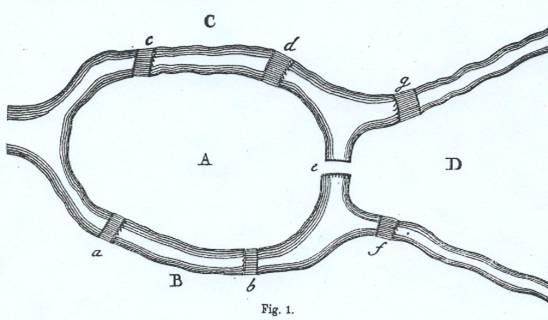
\includegraphics[scale=0.5]{img/koenigsberg.jpg}
\end{center}
L'illustration ci-dessus représente le plan de la ville de Königsberg (de nos jours, Kaliningrad) : la ville est traversée par plusieurs bras d'un fleuve et les quatre quartiers ($A$, $B$, $C$ et $D$) sont reliés par sept ponts notés $a$, $b$, ... $g$. On souhaite répondre à la question suivante : 
\begin{center}
\textbf{Peut-on se promener dans la ville de sorte à traverser chaque pont exactement une fois ?}
\end{center}
Les deux exercices suivants permettent de répondre à cette question, en utilisant des graphes. \textbf{Attention, on autorise les  arêtes multiples.}

%%%%%%%%%%%%%%%%%
\begin{exo}[Graphes eulériens, théorème d'Euler-Hierholzer]
\label{EXO:grapheul}
Un chemin \textbf{eulérien} dans un graphe est un chemin qui passe par chaque arête exactement une fois. Un graphe est \textbf{eulérien} s'il possède un chemin eulérien \textbf{fermé}. Montrer que c'est le cas si et seulement s'il est connexe et que tous ses sommets sont de degré pair.

\begin{hint}
Si, dans un graphe dont les sommets sont tous de degré pair, on retire les arêtes d'un cycle, qu'obtient-on  ? 
\end{hint}
\begin{sol}
La condition est nécessaire parce que si un tel chemin fermé existe, alors les sommets sont forcément de degré pair : à chaque fois que le chemin arrive en un sommet, il en repart.
Montrons que la condition est suffisante. Il y a une preuve par l'absurde, mais voici une preuve constructive. 

Choisissons un sommet $A_1$ et construisons un chemin $c_1$ sur le graphe, en imposant de ne jamais repasser par une arête déjà utilisée, jusqu'à retomber sur $A_1$. Ceci est possible car les degré des sommets sont pairs, donc on ne peut rester bloqué à aucun sommet : s'il y a un moyen d'arriver à un sommet, il y a un moyen d'en repartir et le nombre d'arêtes adjacentes à ce sommet et inutilisées est toujours pair.

Si $c_1$ utilise toutes les arêtes du graphe, on a gagné. Sinon, comme le graphe est connexe, il existe un sommet $A_2$  du chemin $c_1$ dont toutes les arêtes n'ont pas été utilisées (et son nombre d'arêtes non utilisées est pair). On commence un nouveau chemin $\tilde c_2$ en partant de $A_2$ et en n'utilisant que les arêtes non encore utilisées, jusqu'à retomber sur $A_2$. En insérant $\tilde c_2$ dans $c_1$ au point $A_2$, on obtient un nouveau circuit $c_2$ qui ne contient pas deux fois la même arête et qui contient strictement plus d'arêtes que $c_1$. 

Tant qu'on n'a pas utilisé toutes les arêtes, on recommence. Comme le nombre d'arête est fini, et que le nombre d'arêtes libres diminue strictement à chaque étape, il vient un moment où le graphe est entièrement couvert par une marche fermée eulérienne. Cet algorithme est dû à Hierholzer (1873) qui a publié la première preuve rigoureuse du résultat.

%Choisissons un sommet et commençons une marche sur le graphe, en imposant de ne jamais repasser par une arête déjà utilisée, jusqu'à retomber sur le sommet de départ. Ceci est possible car les degré des sommets sont pairs, donc on ne peut rester bloqué à aucun sommet : s'il y a un moyen d'arriver à un sommet, il y a un moyen d'en repartir et le nombre d'arêtes adjacentes à ce sommet et inutilisées est toujours pair.
%
%Si cette marche ne couvre pas tout le graphe, on considère un sommet de la marche qui est adjacent à un sommet non utilisé (donc au moins deux). On relance une marche à partir de ce sommet.
%
%Comme le nombre d'arêtes libres diminue strictement à chaque étape, il vient un moment où le graphe est entièrement couvert par une marche fermée eulérienne. Cet algorithme est dû à Hierholzer qui a publié la première preuve rigoureuse du résultat.


\end{sol}

\end{exo}

%%%%%%%%%%%%%%%%%
\begin{exo}[Graphes semi-eulériens]
 Un graphe est dit \textbf{semi-eulérien} s'il possède un chemin eulérien (c'est-à-dire un chemin passant par chaque arête exactement une fois). Montrer qu'un graphe est semi-eulérien si et seulement si le nombre de ses sommets de degré impair est égal à $0$, ou $2$. 

Que peut-on en déduire à propos des ponts de Königsberg ?
% pas possible : il y a quatre sommets impairs.
\begin{hint}
S'il y a deux sommets de degré impair, ajouter une arête entre ces deux sommets.
\end{hint}
\begin{sol}
Supposons qu'il existe un chemin eulérien. Si c'est un cycle, l'exercice \ref{EXO:grapheul} assure que 
tous les sommets sont de degrés pairs. Si ce n'est pas un chemin fermé, alors les sommets qui ne sont pas à ses extrémités sont forcément de degré pair : à chaque fois que le chemin arrive en un sommet, il en repart. Et les extrémités sont de degré impair.

Réciproquement, notons $N$ le nombre de sommets de degré impair.

$\bullet$ Si $N=0$, le graphe est eulérien, donc en particulier semi-eulérien.

$\bullet$ Si $N=2$, rajoutons une arête entre les deux sommets en question : les degrés des deux sommets en question augmentent chacun de  un, donc deviennent pairs. Par l'exercice \ref{EXO:grapheul}, le graphe devient eulérien . Il existe alors un chemin eulérien fermé . Ensuite, on enlève l'arête ajoutée, ce qui donne un chemin eulérien (non fermé).

Pour les ponts de Königsberg, on en déduit que c'est impossible : le graphe n'est pas semi-eulérien, car il a quatre sommets impairs.

%Notons $N$ le nombre de sommets de degré impair.
%Si $N=0$, le graphe est eulérien, donc en particulier semi-eulérien.
%
%Si $N=2$, rajoutons une arête entre les deux sommets en question : les degrés des deux sommets en question augmentent chacun de  un, donc deviennent pairs. Par l'exercice précédent, le graphe devient eulérien . Il existe alors un chemin eulérien fermé . Ensuite, on enlève l'arête ajoutée, ce qui donne un chemin eulérien (non fermé).
%
%Pour les ponts de Königsberg, on en déduit que c'est impossible : le graphe n'est pas semi-eulérien, car il a quatre sommets impairs.
\end{sol}
\end{exo}



%%%%%%%%%%%%%%%%%%%%%%%%%%%%%
%\chapter{Graphes, bis}
%%%%%%%%%%%%%%%%%%%%%%%%%%%%%


%%%%%%%%%%%%%%%%%
\begin{exo}[Composantes connexes]
Soit $G$ un graphe à $s$ sommets,  $a$ arêtes, et $k$ composantes connexes.
\begin{enumerate}
\item Montrer que $s \leq a+k$. 
\item Quand y a-t-il égalité ? 
\end{enumerate}
\begin{hint}
\begin{enumerate}
\item Procéder par récurrence sur le nombre d'arêtes du graphe.
\item On pourra considérer le cas $k=1$, et  interpréter dans ce cas la quantité $a-s+1$.% C'est le nombre de cycles élémentaires : un arbre couvrant possède $s-1$ arêtes : donc $a-(s-1)$ est le nombre d'arêtes ajoutées à un arbre couvrant.
\end{enumerate}
\end{hint}
\begin{sol}
\begin{enumerate}
\item Notons, pour tout entier $a$ naturel, $P(a)$ l'assertion suivante: \og Tout arbre ayant $a$ arêtes vérifie l'inégalité $s \leq a+k$, avec $k$ le nombre de composantes connexes du graphe et $s$ son nombre de sommets.\fg{} Montrons que $P(a)$ est vraie pour tout $a$, par récurrence.\\
\textbf{Initialisation.} Pour $a=0$, on a $s=k$ donc $s\leq a+k$.\\
\textbf{Hérédité.} Soit $a\in \N$. Supposons que $P(a)$ soit vraie. Démontrons $P(a+1)$.  Soit $G$ un graphe ayant $a+1$ arêtes. Notons $k$ le nombre de ses composantes connexes et $s$ le nombre de ses sommets. Si on enlève une arête de ce graphe, on obtient un sous-graphe $G'$ ayant $a$ arêtes. En ce qui concerne les composantes connexes, il y a deux cas :
\begin{itemize}
\item Soit $G'$ a toujours $k$ composantes connexes. Dans ce cas, par hypothèse de récurrence appliquée à $G'$, on a  $s\leq a+k$ donc forcément  $s\leq (a+1)+k$.
\item Soit $G'$ a $k+1$ composantes connexes. Dans ce cas, par hypothèse de récurrence appliquée à $G'$, on a $s \leq a+ (k+1) = (a+1)+k$.
\end{itemize}
Dans les deux cas, on a bien $s\leq (a+1)+k$. Donc $P(a+1)$ est vraie.\\
Par le principe de récurrence, ceci montre que pour tout graphe ayant $s$ sommets, $a$ arêtes et $k$ composantes connexes, on a $s\leq a+k$.
\item Il y a égalité ssi le graphe est une union disjointe d'arbres.
\end{enumerate}
\end{sol}
\end{exo}

%%%%%%%%%%%%%%%%%
\begin{exo}[Quatre sommets de chaque degré]
Soit $G$ un graphe dont on note $a$ le nombre d'arêtes, et $l$ un entier naturel. On suppose que pour tout naturel $k\leq l$, $G$ possède exactement quatre sommets de degré $k$. Montrer que $l\leq \sqrt a$.
\begin{hint}
Que vaut la quantité $0+1+2+3+...+l$ ?
\end{hint}
\begin{sol}
On sait que $2a$ est égal à la somme des degrés de tous les sommets. Or, cette somme vaut au moins $4\times0+4\times 1+4\times 2 ... + 4\times l$ (plus les degrés supérieurs à $l$). Donc cette somme vaut au moins $4(0+1+2+...+l) = 4\frac{l(l+1)}{2} = 2l(l+1)$. En en déduit que $a \geq l(l+1) \geq l^2$, ce qui donne $l\leq \sqrt a$.
\end{sol}
\end{exo}

%%%%%%%%%%%%%%%%%
\begin{exo}[Graphes orientés]
Cinq amis jouent des parties d'échecs. En tout, quatorze parties sont jouées. Montrer qu'au moins une des personnes a perdu au plus deux parties.
\begin{sol}
Supposons par l'absurde le contraire, c'est-à-dire que tout le monde a perdu au moins trois parties. La situation est modélisée par un graphe orienté à cinq sommets et quatorze arêtes orientées, sachant qu'une arête orientée $(s,s')$ correspond à une partie jouée entre $s$ et $s'$ et gagnée par $s$.

Considérons la somme, pour tous les sommets, du nombre d'arêtes entrantes du sommet, c'est-à-dire du nombre de parties perdues par chaque joueur. Ce nombre est égal au nombre total de parties, donc $14$ (ou moins s'il y a des parties nulles). D'autre part si tout le monde a perdu au moins trois parties, ce nombre doit être au moins égal à $3\times 5=15$, ce qui est absurde.

Remarque : la technique utilisée est la version orientée de $\sum_{x\in S}\operatorname{deg}(x) = 2a$.
\end{sol}
\end{exo}

%%%%%%%%%%%%%%%%%
\begin{exo}[Nombre de connaissances]
% Garet ex 1.7, chercher d'autres preuves, par exemple par récurrence ?
Au cours d'une réunion rassemblant $n\geq 4$ personnes, on se rend compte que dans chaque groupe de quatre personnes, il y en a au moins une qui connaît les trois autres. Montrer qu'il existe au moins $n-3$ personnes qui connaissent tout le monde.
\begin{sol}
Il s'agit de montrer qu'au moins $n-3$ des degrés valent $n-1$.

\textbf{Première preuve.} Supposons que l'ensemble des points de degré $\leq n-2$, c'est-à-dire non reliés à tous les autres, soit de cardinal plus de quatre.

Prenons quatre points dans cet ensemble de sorte que $A$ et $B$ ne soient pas reliés, et $C$ et $D$ ne soient pas reliés (justifier que c'est possible). Contradiction avec l'hypothèse.

\textbf{Deuxième preuve, avec le graphe complémentaire. } Dans le graphe complémentaire $G^c$ (celui avec les mêmes sommets, et avec des arêtes exactement là où $G$ n'en avait pas), il s'agit de montrer qu'il y a au moins $n-3$ points isolés, donc que l'ensemble des composantes connexes non triviales comporte moins de trois sommets.

L'hypothèse elle, est que sur tout sous-ensemble de quatre sommets, au moins un sommet est relié aux trois autres, donc, en ce qui concerne le graphe dual, que pour tout sous-ensemble de quatre sommets, il y a au moins un point isolé \emph{dans ce sous-graphe de quatre sommets} (pas forcément isolé dans $G^c$).

Or, si l'ensemble des composantes connexes a plus de quatre sommets, on peut trouver $A$, $B$, $C$ et $D$ tels que $A$ et $B$ sont adjacents, et $C$ et $D$ aussi. Dans le sous-graphe formé par ces quatre points, il n'y pas de point isolé, contradiction.

\end{sol}
\end{exo}

%%%%%%%%%%%%%%%%%
\begin{exo}[Degrés possibles (vers Erdős–Gallai)]
% Olivier ex 11 p. 16
À la fin d'une réception, on demande aux participants avec combien de personnes ils ont discuté. On obtient comme réponses : $7, 6, 5, 4, 3, 3, 2$. Montrer qu'au moins une personne a fait une erreur.
% pas le bon nombre de personnes, 7 impossible sinon il y aurait 8 personnes.
Même question avec :
\begin{itemize}
\item $7,6,5,4,3,3,2,1$; % somme impaire, impossible
\item $7,7,5,4,3,3,2,1$;% deux qui connaissent tt le monde, un autre qui ne connaît qu'une personne, impossible
\item $7,7,6,4,3,3,2,2$. % ?
%\item $6,6,4,2,2,2,2,2$; % ?
\end{itemize}
\begin{sol}
Pour le premier, il y a sept personnes, personne ne peut avoir discuté avec sept interlocuteurs.

Pour le deuxième, la somme des degrés est impaire, alors qu'elle devrait être paire.

Pour le troisième, il y a deux personnes qui connaissent tout le monde, or la dernière personne ne connaît qu'une personne, impossible.

Pour la dernière, c'est plus compliqué. Considérons les arêtes adjacentes aux trois premiers sommets. Ces arêtes aboutissent soit à ces trois sommets, soit aux autres. Mais pour chacun des autres points, il ne peut y avoir que $min(3,d_i)$ arêtes qui partent vers les trois premiers sommets au maximum.

La quantité $d_1+d_2+d_3$ est égale à $2$(arêtes entre les trois premiers sommets)$+$(arêtes entre les trois premiers sommets et les suivants), et est donc bornée par $6+\sum_{i=4}^n \min(3,d_i)$.

Ici, on obtient $7+7+6=20 \leq 6 + 3+3+3+2+2=19$, contradiction.

De façon générale, on doit avoir:
\[ \forall k\leq n, \sum_{i=1}^k d_i \leq k(k-1) + \sum_{i=k+1}^n \min(k,d_i).\] 
C'est le théorème d'Erdős–Gallai. La preuve est une généralisation de l'argument expliqué ci-dessus. Voir \url{https://en.wikipedia.org/wiki/Erd%C5%91s%E2%80%93Gallai_theorem}
\end{sol}
\end{exo}

%Comparaison de construction d'arbres couvrants : en largeur, en profondeur, propriétés sur la distance, voir x-ups.


% ATTENTION enlever ???
%%%%%%%%%%%%%%%%%
\begin{exo}[Distance géodésique]
Proposer un algorithme pour calculer la distance géodésique entre deux points dans un graphe.
\begin{sol}
Une solution est de construire un arbre couvrant de $G$ par exploration en largeur à partir de $x$ : une branche de l'arbre finit par contenir $y$ et le chemin dans l'arbre est un chemin de longueur minimale.
\end{sol}
\end{exo}

% autres exos possibles : algo pour trouver le diamètre d'un arbre : commencer d'un point $s$, trouver le point $u$ le plus lointain, puis commencer de $u$, trouver le point $v$ le plus lointain : ça marche.
% la preuve utilise l'inégalité triangulaire 
% rédiger ça dans un contexte non-math.

% algo pour trouver le diamètre d'un graphe, sans matrices.

%\chapter*{$k$-connexité}

%Plus de choses sur le théorème de Menger ?

%Utile aussi pour Kuratowski



%Théorème d'Erdös-Gallai sur la condition pour une suite de degré pour être la suite de degrés d'un graphe. ?

%Graphes biparti (=2-coloriable)

%Problèmes de coloriage



%%%%%%%%%%%%%%%%%
\begin{exo}[Graphes hamiltoniens]
On appelle chemin hamiltonien (en l'honneur de Hamilton) un chemin contenant chaque sommet exactement une fois. Un cycle hamiltonien est un cycle qui devient un chemin hamiltonien lorsqu'on enlève une arête. Un graphe est dit \textbf{hamiltonien} s'il contient un cycle hamiltonien.
\begin{enumerate}
\item Montrer que le graphe d'un cube est hamiltonien. Plus généralement, montrer que le graphe d'un des cinq solides platoniciens est hamiltonien. Bonus : c'est également vrai pour les treize solides archimédiens.% Garner, 1957 ?
\item Montrer qu'un graphe complet est Hamiltonien.
\item Montrer qu'un tournoi, c'est-à-dire un graphe complet \textbf{orienté}, contient un chemin hamiltonien orienté (Théorème de Rédei, 1934). % dja, feuille récurrence bis
% If the sums of the degrees of nonadjacent vertices in a graph G is greater than the number of nodes n for all subsets of nonadjacent vertices, then G is Hamiltonian (Ore 1960; Skiena 1990, p. 197).
% graphes biparti avec unbalanced vertex parity -> pas hamiltonien
\end{enumerate}
\begin{sol}
\begin{enumerate}
\item\begin{center}
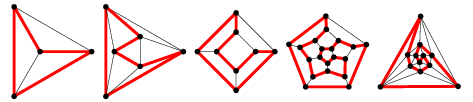
\includegraphics[scale=0.5]{img/PlatonicHamiltonian.png}
\end{center}
\item Soit $n$ le nombre de sommets du graphe. Les sommets sont tous de degré $n-1$. D'après un exercice de la feuille $1$, il existe un cycle de longueur $n$, que l'on peut construire étape par étape, en partant de n'importe quel sommet. A l'étape $k$, avec $1\leq k\leq n-1$, on dispose donc d'un chemin élémentaire ayant $k$ sommets distincts. Parmi les $n-1$ sommets adjacents du dernier sommet, il y a les $k-1$ prédécesseurs du dernier sommet, on choisit un successeur parmi les $n-k$ voisins restants. Ceci construit un chemin hamiltonien passant par tous les sommets. Comme le graphe est complet, on peut relier le premier au dernier point, ce qui donne un cycle hamiltonien.
\item Par récurrence sur le nombre de sommets.
\end{enumerate}
\end{sol}
\end{exo}

%%%%%%%%%%%%%%%%%
\begin{exo}[Dominos]
% Garet ex. 15
% (Un graphe complet est hamiltonien)
Peut-on aligner tous les pions du jeu de domino suivant la règle du jeu de domino ? Le jeu du domino à $n$ valeurs est composé de $n$ doubles du type $(i,i)$, et de $n(n-1)/2$ paires $(i,j)$ avec $i\neq j$, ce qui fait au total $n(n+1)/2$ pièces. Pour $n=6$, on retrouve le jeu de domino classique.
\begin{center}
\begin{tikzpicture}[line cap=round,line join=round,>=triangle 45,x=1.0cm,y=1.0cm]
\clip(-0.2,-0.2) rectangle (2.2,2.2);
\draw (0,0)-- (2,0);
\draw (2,0)-- (2,1);
\draw (2,1)-- (0,1);
\draw (0,1)-- (0,0);
\draw (1,0.1)-- (1,0.9);
\begin{scriptsize}
\draw [fill=black] (0.3,0.3) circle (2pt);
\draw [fill=black] (0.5,0.5) circle (2pt);
\draw [fill=black] (0.7,0.7) circle (2pt);
\draw [fill=black] (1.5,0.5) circle (2pt);
\end{scriptsize}
\end{tikzpicture}
\end{center}
\begin{hint}
Il suffit de résoudre le problème sans les doubles, que l'on peut intercaler par la suite.

%Sans les doubles, on se retrouve avec un graphe complet, et un graphe complet est hamiltonien.
% ATTENTION, ERREUR ? Voir remarque de Tom et Clémence, refaire.
\end{hint}
\end{exo}
\newpage

%%%%%%%%%%%%%%%%%
\begin{exo}[Lemme de Sperner]
Le but de cet exercice est de démontrer le :
\begin{theoreme}[\og Lemme de Sperner\fg{} en dimension deux, 1928]
Soit $ABC$ un triangle, muni d'une triangulation. Les sommets de la triangulation sont coloriés avec trois couleurs, de telle sorte que:
\begin{enumerate}
\item $A$, $B$ et $C$ sont de couleur $1$, $2$ et $3$.
\item Les sommets situés sur un côté de $ABC$ sont coloriés avec une des deux couleurs des extrémités de ce segment. Par exemple, un sommet situé sur $[BC]$ est de couleur $2$ ou $3$.
\end{enumerate}
Alors, il existe un triangle de la triangulation dont les sommets sont coloriés avec les trois couleurs. Plus précisément, il existe un nombre impair de tels triangles.
\end{theoreme}

Pour démontrer ce résultat, on introduit un graphe de la façon suivante : 
\begin{itemize}
\item les sommets sont les régions délimitées par la triangulation (y compris la région extérieure);
\item deux sommets du graphe sont reliés par une arête si les régions correspondantes ont une frontière commune, et si cette frontière a des extrémités coloriées $1$ et $2$.
\end{itemize}
En considérant la parité des sommets du graphe (d'une part le sommet extérieur, et d'autre part les sommets intérieurs), démontrer le théorème.
\begin{sol}
Sur le côté $[AB]$ du triangle, les couleurs des sommets de la triangulation changent un nombre impair de fois (autrement, les couleurs de $A$ et $B$ seraient les mêmes).

On en déduit que le sommet du graphe extérieur au triangle est de degré impair.

Or, on sait que dans un graphe, le nombre de sommets de degré impair est pair. Il reste donc un nombre impair de sommets impairs à l'intérieur du triangle.

Dans le triangle, le degré d'un sommet peut être $0$, $1$ ou $2$ mais pas $3$, et le cas du degré $1$ correspond au cas d'un triangle dont les sommets sont de trois couleurs distinctes. C'est aussi le seul cas où le degré est impair.

On en déduit qu'il existe à l'intérieur du triangle un nombre impair de sommets du graphe de degré $1$, et donc qu'il existe dans le triangle $ABC$ un nombre impair de triangles tricolores.
\end{sol}
\end{exo}





%%%%%%%%%%%%%%%%%%%%%%%%%%%%%
\chapter{Chasse aux angles}
%%%%%%%%%%%%%%%%%%%%%%%%%%%%%
\definecolor{qqwuqq}{rgb}{0,0.39,0}
\definecolor{uuuuuu}{rgb}{0.27,0.27,0.27}
\definecolor{xdxdff}{rgb}{0.49,0.49,1}
\definecolor{qqqqff}{rgb}{0,0,1}
\definecolor{ffqqqq}{rgb}{1.,0.,0.}

%%%%%%%%%%%%%%%%%
\begin{exo}[Octogone appuyé sur un segment]
%exo7
% angle au centre, inscrit. application directe
Construire un octogone convexe régulier dont un des côtés est un segment $[AB]$ donné.

\begin{hint}   
Il y a deux tels octogones. En notant $O$ le centre d'un tel octogone, on doit avoir $\widehat{AOB}=\pm \pi/4$.
\end{hint}      
\begin{sol}  
Construisons un triangle $AIB$ isocèle rectangle en $I$ et le cercle de centre $I$ et de rayon $IA$. Ce cercle intersecte la médiatrice de $[AB]$ en un point $O$ qui vérifie $\widehat{AOB}=\pm \pi/4$, par le théorème de l'angle au centre. C'est donc le centre d'un octogone appuyé sur $[AB]$. En traçant le cercle de centre $O$ et de rayon $OA$, on peut terminer la construction de cet octogone.
\end{sol}  
\end{exo}  


%%%%%%%%%%%%%%%%%
\begin{exo}[Trapèzes inscriptibles] % exo7
% angles inscrits, facile, application directe
Montrer qu'un trapèze est isocèle si et seulement s'il est inscriptible.


\begin{sol}
Commençons par rappeler deux points:
\begin{enumerate}
\item dans un trapèze, deux angles non adjacents à une même base sont supplémentaires, puisque les deux bases sont parallèles.
\item un quadrilatère non croisé est inscriptible ssi les angles opposés sont supplémentaires.
\end{enumerate}

Un trapèze est isocèle ssi les angles adjacents à une même base sont égaux, donc (par le premier point ci-dessus) ssi les angles opposés sont supplémentaires, donc (par le deuxième point) ssi il est inscriptible.

\begin{center}
\definecolor{qqwuqq}{rgb}{0.,0.39215686274509803,0.}
\definecolor{uuuuuu}{rgb}{0.26666666666666666,0.26666666666666666,0.26666666666666666}
\definecolor{qqqqff}{rgb}{0.,0.,1.}
\begin{tikzpicture}[line cap=round,line join=round,>=triangle 45,x=1.0cm,y=1.0cm]
\clip(-1.76,-0.56) rectangle (4.66,5.42);
\draw [shift={(1.94,4.96)},color=qqwuqq,fill=qqwuqq,fill opacity=0.1] (0,0) -- (-149.61179814845522:0.6) arc (-149.61179814845522:-47.299703593483734:0.6) -- cycle;
\draw [shift={(-0.36,0.18)},color=qqwuqq,fill=qqwuqq,fill opacity=0.1] (0,0) -- (30.388201851544782:0.6) arc (30.388201851544782:108.07610729657328:0.6) -- cycle;
\draw [shift={(-1.3,3.06)},color=qqwuqq,fill=qqwuqq,fill opacity=0.1] (0,0) -- (-71.92389270342673:0.6) arc (-71.92389270342673:30.388201851544792:0.6) -- cycle;
\draw(1.3116327852336915,2.319005145180441) circle (2.71471898725753cm);
\draw (-1.3,3.06)-- (1.94,4.96);
\draw (-1.3,3.06)-- (-0.36,0.18);
\draw (-0.36,0.18)-- (3.9945107601576444,2.7335711247838033);
\draw (3.9945107601576444,2.7335711247838033)-- (1.94,4.96);
\draw [shift={(-0.36,0.18)},color=qqwuqq] (30.388201851544782:0.6) arc (30.388201851544782:108.07610729657328:0.6);
\draw [shift={(-0.36,0.18)},color=qqwuqq] (30.388201851544782:0.5) arc (30.388201851544782:108.07610729657328:0.5);
\begin{scriptsize}
\draw [fill=qqqqff] (-0.36,0.18) circle (2.5pt);
\draw[color=qqqqff] (-0.74,-0.01) node {$A$};
\draw [fill=qqqqff] (-1.3,3.06) circle (2.5pt);
\draw[color=qqqqff] (-1.64,3.33) node {$B$};
\draw [fill=qqqqff] (1.94,4.96) circle (2.5pt);
\draw[color=qqqqff] (2.08,5.27) node {$C$};
\draw [fill=uuuuuu] (3.9945107601576444,2.7335711247838033) circle (1.5pt);
\draw[color=uuuuuu] (4.28,2.81) node {$D$};
\end{scriptsize}
\end{tikzpicture}
\end{center}

\end{sol}
\end{exo}  


%%%%%%%%%%%%%%%%%
\begin{exo}[Antiparallélogramme]
%exo7
% angles inscrits
Un antiparallélogramme est un quadrilatère croisé dont les cotés opposés sont deux à deux de même longueur. Soit $ABCD$ un antiparallélogramme. Montrer les assertion suivantes.

\begin{center}
\definecolor{uuuuuu}{rgb}{0.26666666666666666,0.26666666666666666,0.26666666666666666}
\definecolor{qqqqff}{rgb}{0.,0.,1.}
\begin{tikzpicture}[line cap=round,line join=round,>=triangle 45,x=1.0cm,y=1.0cm]
\clip(-1.76,-0.56) rectangle (4.66,5.42);
\draw (-0.36,0.18)-- (1.94,4.96);
\draw (-1.3,3.06)-- (3.9945107601576444,2.7335711247838033);
\draw (-1.3,3.06)-- (-0.36,0.18);
\draw (1.94,4.96)-- (3.9945107601576444,2.7335711247838033);
\begin{scriptsize}
\draw [fill=qqqqff] (-0.36,0.18) circle (2.5pt);
\draw[color=qqqqff] (-0.74,-0.01) node {$A$};
\draw [fill=qqqqff] (-1.3,3.06) circle (2.5pt);
\draw[color=qqqqff] (-1.64,3.33) node {$D$};
\draw [fill=qqqqff] (1.94,4.96) circle (2.5pt);
\draw[color=qqqqff] (2.08,5.27) node {$B$};
\draw [fill=uuuuuu] (3.9945107601576444,2.7335711247838033) circle (1.5pt);
\draw[color=uuuuuu] (4.28,2.81) node {$C$};
\end{scriptsize}
\end{tikzpicture}
\end{center}

\begin{enumerate}
\item Les angles opposés ont la même mesure.
\item Les diagonales $(AC)$ et $(BD)$ sont parallèles.
\item La médiatrice des diagonales est un axe de symétrie de $ABCD$.
\item Deux côtés opposés ont leur point d'intersection situé sur cette médiatrice.
\item Le quadrilatère convexe $ADBC$ formé par les deux côtés non croisés et les diagonales est un trapèze isocèle.
\item $ABCD$ est inscriptible.
\end{enumerate}


\end{exo}  

%------------------
%%%%%%%%%%%%%%%%%
\begin{exo}[Théorème de Reim]
% nom : Th de Reim
% source :  OFM 2014-2015 envoi 2 (22 pages) exercice 3.7
% via Budzinski
% voir aussi http://www.debart.fr/pdf/cercle_seconde.pdf
Soient $\mathcal C_1$ et $\mathcal C_2$ deux cercles sécants en $A$ et $B$, et $\mathcal D_A$ (respectivement $\mathcal D_B$) une droite passant par $A$  (resp. $B$). On note $C$ et $E$ (resp. $D$ et $F$) l'intersection de $\mathcal D_A$ (resp. $\mathcal D_B$) avec 
 les deux cercles. Montrer que $(CD) // (EF)$.
 \begin{center}
\begin{tikzpicture}[line cap=round,line join=round,>=triangle 45,x=1.0cm,y=1.0cm]
\clip(-6.84,-1.3) rectangle (3.34,5.62);
%\draw [shift={(-4.54135770173771,2.073391502619976)},color=qqwuqq,fill=qqwuqq,fill opacity=0.1] (0,0) -- (-57.19135026317228:0.6) arc (-57.19135026317228:19.883254180671244:0.6) -- cycle;
%\draw [shift={(-0.9357905924919852,-0.14942814068146326)},color=qqwuqq,fill=qqwuqq,pattern=north east lines,pattern color=qqwuqq] (0,0) -- (76.27770286686645:0.5) arc (76.27770286686645:179.20309842302296:0.5) -- cycle;
%\draw [shift={(-1.7679241049654213,3.0764437353898777)},color=qqwuqq,fill=qqwuqq,fill opacity=0.1] (0,0) -- (-57.191350263172325:0.6) arc (-57.191350263172325:19.88325418067124:0.6) -- cycle;
%\draw [shift={(-0.9357905924919852,-0.14942814068146326)},color=qqwuqq,fill=qqwuqq,fill opacity=0.1] (0,0) -- (-0.7969015769770713:0.6) arc (-0.7969015769770713:76.27770286686646:0.6) -- cycle;
\draw(-2.,2.16) circle (2.5428330656966063cm);
\draw(-0.28,1.74) circle (2.cm);
\draw [domain=-6.84:3.34] plot(\x,{(--9.256772261245349--0.9009661428453959*\x)/2.4911661511599217});
\draw [domain=-6.84:3.34] plot(\x,{(-0.5906140983383479-0.05057185931853675*\x)/3.6357905924919853});
\draw [color=ffqqqq,domain=-6.84:3.34] plot(\x,{(-7.025760591657469-2.192326777340297*\x)/1.4133266677517589});
\draw [color=ffqqqq,domain=-6.84:3.34] plot(\x,{(-0.6985138943712147--3.2433807595236943*\x)/-2.090909333629991});
%\draw [dash pattern=on 3pt off 3pt] (-0.9357905924919852,-0.14942814068146326)-- (0.008833848840078207,3.719033857154604);
\begin{scriptsize}
\draw [fill=uuuuuu] (0.008833848840078207,3.719033857154604) circle (1.5pt);
\draw[color=uuuuuu] (0.12,4.12) node {$A$};
\draw [fill=uuuuuu] (-0.9357905924919852,-0.14942814068146326) circle (1.5pt);
\draw[color=uuuuuu] (-0.92,-0.4) node {$B$};
\draw [fill=uuuuuu] (-4.54135770173771,2.073391502619976) circle (1.5pt);
\draw[color=uuuuuu] (-4.96,2.32) node {$C$};
\draw [fill=uuuuuu] (-3.1280310339859514,-0.11893527472032112) circle (1.5pt);
\draw[color=uuuuuu] (-3.24,-0.3) node {$D$};
\draw [fill=uuuuuu] (-1.7679241049654213,3.0764437353898777) circle (1.5pt);
\draw[color=uuuuuu] (-1.72,3.56) node {$E$};
\draw [fill=uuuuuu] (0.32298522866456997,-0.1669370241338166) circle (1.5pt);
\draw[color=uuuuuu] (0.28,-0.4) node {$F$};
\end{scriptsize}
\end{tikzpicture}
\end{center}
\begin{sol}
Traçons une figure. \emph{On marque dès à présent quelques égalités d'angles obtenues par le théorème de l'angle inscrit:}

\begin{center}
\begin{tikzpicture}[line cap=round,line join=round,>=triangle 45,x=1.0cm,y=1.0cm]
\clip(-6.84,-1.3) rectangle (3.34,5.62);
\draw [shift={(-4.54135770173771,2.073391502619976)},color=qqwuqq,fill=qqwuqq,fill opacity=0.1] (0,0) -- (-57.19135026317228:0.6) arc (-57.19135026317228:19.883254180671244:0.6) -- cycle;
\draw [shift={(-0.9357905924919852,-0.14942814068146326)},color=qqwuqq,fill=qqwuqq,pattern=north east lines,pattern color=qqwuqq] (0,0) -- (76.27770286686645:0.5) arc (76.27770286686645:179.20309842302296:0.5) -- cycle;
\draw [shift={(-1.7679241049654213,3.0764437353898777)},color=qqwuqq,fill=qqwuqq,fill opacity=0.1] (0,0) -- (-57.191350263172325:0.6) arc (-57.191350263172325:19.88325418067124:0.6) -- cycle;
\draw [shift={(-0.9357905924919852,-0.14942814068146326)},color=qqwuqq,fill=qqwuqq,fill opacity=0.1] (0,0) -- (-0.7969015769770713:0.6) arc (-0.7969015769770713:76.27770286686646:0.6) -- cycle;
\draw(-2.,2.16) circle (2.5428330656966063cm);
\draw(-0.28,1.74) circle (2.cm);
\draw [domain=-6.84:3.34] plot(\x,{(--9.256772261245349--0.9009661428453959*\x)/2.4911661511599217});
\draw [domain=-6.84:3.34] plot(\x,{(-0.5906140983383479-0.05057185931853675*\x)/3.6357905924919853});
\draw [color=ffqqqq,domain=-6.84:3.34] plot(\x,{(-7.025760591657469-2.192326777340297*\x)/1.4133266677517589});
\draw [color=ffqqqq,domain=-6.84:3.34] plot(\x,{(-0.6985138943712147--3.2433807595236943*\x)/-2.090909333629991});
\draw [dash pattern=on 3pt off 3pt] (-0.9357905924919852,-0.14942814068146326)-- (0.008833848840078207,3.719033857154604);
\begin{scriptsize}
\draw [fill=uuuuuu] (0.008833848840078207,3.719033857154604) circle (1.5pt);
\draw[color=uuuuuu] (0.12,4.12) node {$A$};
\draw [fill=uuuuuu] (-0.9357905924919852,-0.14942814068146326) circle (1.5pt);
\draw[color=uuuuuu] (-0.92,-0.4) node {$B$};
\draw [fill=uuuuuu] (-4.54135770173771,2.073391502619976) circle (1.5pt);
\draw[color=uuuuuu] (-4.96,2.32) node {$C$};
\draw [fill=uuuuuu] (-3.1280310339859514,-0.11893527472032112) circle (1.5pt);
\draw[color=uuuuuu] (-3.24,-0.3) node {$D$};
\draw [fill=uuuuuu] (-1.7679241049654213,3.0764437353898777) circle (1.5pt);
\draw[color=uuuuuu] (-1.72,3.56) node {$E$};
\draw [fill=uuuuuu] (0.32298522866456997,-0.1669370241338166) circle (1.5pt);
\draw[color=uuuuuu] (0.28,-0.4) node {$F$};
\end{scriptsize}
\end{tikzpicture}
\end{center}

\emph{Les égalités d'angles repérées sur la figure permettent de voir la solution, au moins dans la configuration particulière dessinée. On voit en effet que les angles $\widehat{ECD}$ et $\widehat{AEF}$ sont égaux. Attention toutefois, les angles géométriques sont trompeurs et les égalités que l'on voit sur une figure peuvent dépendre de la façon de tracer la figure. Sur la figure ci-dessous par exemple, les angles en question ne sont pas égaux mais supplémentaires.}

\begin{center}
\begin{tikzpicture}[line cap=round,line join=round,>=triangle 45,x=1.0cm,y=1.0cm]
\clip(-6.82,-1.14) rectangle (3.36,5.7);
\draw [shift={(-3.11,4.35)},color=qqwuqq,fill=qqwuqq,fill opacity=0.1] (0,0) -- (-111.67:0.6) arc (-111.67:-15.58:0.6) -- cycle;
\draw [shift={(-0.76,1.49)},color=qqwuqq,fill=qqwuqq,pattern=north east lines,pattern color=qqwuqq] (0,0) -- (96.63:0.5) arc (96.63:180.54:0.5) -- cycle;
\draw [shift={(-0.76,1.49)},color=qqwuqq,fill=qqwuqq,fill opacity=0.1] (0,0) -- (0.54:0.6) arc (0.54:96.63:0.6) -- cycle;
\draw [shift={(1.53,3.06)},color=qqwuqq,fill=qqwuqq,pattern=north east lines,pattern color=qqwuqq] (0,0) -- (164.42:0.6) arc (164.42:248.33:0.6) -- cycle;
\draw(-2.52,2.44) circle (2cm);
\draw(0.06,2.74) circle (1.5cm);
\draw [domain=-6.82:3.36] plot(\x,{(--15.16-1.21*\x)/4.35});
\draw [domain=-6.82:3.36] plot(\x,{(--5.5--0.03*\x)/3.68});
\draw [color=ffqqqq,domain=-6.82:3.36] plot(\x,{(-14.02-2.9*\x)/-1.15});
\draw [color=ffqqqq,domain=-6.82:3.36] plot(\x,{(-0.48--1.56*\x)/0.62});
\draw [dash pattern=on 2pt off 2pt] (-0.76,1.49)-- (-1.03,3.77);
\begin{scriptsize}
\draw [fill=uuuuuu] (-1.03,3.77) circle (1.5pt);
\draw[color=uuuuuu] (-0.88,4.16) node {$A$};
\draw [fill=uuuuuu] (-0.76,1.49) circle (1.5pt);
\draw[color=uuuuuu] (-0.74,1.2) node {$B$};
\draw [fill=uuuuuu] (-3.11,4.35) circle (1.5pt);
\draw[color=uuuuuu] (-3.38,4.7) node {$C$};
\draw [fill=uuuuuu] (-4.26,1.45) circle (1.5pt);
\draw[color=uuuuuu] (-4.56,1.28) node {$D$};
\draw [fill=uuuuuu] (1.53,3.06) circle (1.5pt);
\draw[color=uuuuuu] (1.56,3.52) node {$E$};
\draw [fill=uuuuuu] (0.91,1.5) circle (1.5pt);
\draw[color=uuuuuu] (1,1.24) node {$F$};
\end{scriptsize}
\end{tikzpicture}
\end{center}

\emph{Il ne reste plus qu'à rédiger rigoureusement la solution  avec des angles orientés de droites, en s'appuyant sur l'intuition donnée par la figure.}

Pour montrer que $(CD)$ et $(EF)$ sont parallèles, il suffit par exemple de montrer qu'elles forment le même angle avec la droite $(CA)$. Or on a la suite d'égalités d'angles de droites :

\begin{align*}
(CD,CA) &= (BD,BA) \text{ car $CDAB$ est inscriptible}\\
&= (BF,BA) \text{ car $(BD)=(BF)$}\\
&=(EF,EA) \text{ car $BFAE$ est inscriptible}\\
&=(EF,CA)  \text{ car $(EA)=(CA)$.}
\end{align*}

\end{sol} 
\end{exo}


%---------------
%%%%%%%%%%%%%%%%%
\begin{exo}[Bissectrice et médiatrice]
% source : exogeo.pdf Grenoble
% exercice simple sur les angles inscrits
La bissectrice en $A$ d'un triangle quelconque $ABC$ recoupe le cercle $\Gamma$ circonscrit à ce triangle en un point $I$. Montrer que $I$  appartient à la médiatrice de $[BC]$.
\begin{hint}
Montrer que $BIC$ est isocèle en $I$.
\end{hint}

\begin{sol}

Pour montrer le résultat, il suffit de montrer que $IBC$ et $JBC$ sont isocèles en $I$ et $J$.

On rédige avec des angles de droites, ce qui a l'avantage de démontrer simultanément le résultat pour la bissectrice intérieure et extérieure.

En effet, les angles de droites ne voient pas la différence entre une bissectrice intérieure et extérieure : étant données deux droites $\mathcal D$ et $\mathcal D'$, une droite $\Delta$ est une bissectrice si 
\[(\mathcal D,\Delta) = (\Delta,\mathcal D').\]
 Deux droites ont deux bissectrices. On ne peut distinguer les deux bissectrices que si on fixe des vecteurs directeurs des droites.

On prend donc une bissectrice (intérieure sur la figure mais ça ne changera rien), et on marque les angles égaux sur la figure :

\begin{tikzpicture}[line cap=round,line join=round,>=triangle 45,x=0.6235592739369882cm,y=0.6235592739369843cm]
\clip(1.98,-10.03) rectangle (18.02,6.01);
\draw [shift={(15.92,-5.44)},color=qqwuqq,fill=qqwuqq,fill opacity=0.1] (0,0) -- (180.39:1.24) arc (180.39:214.67:1.24) -- cycle;
\draw [shift={(8.29,2.24)},color=qqwuqq,fill=qqwuqq,fill opacity=0.1] (0,0) -- (-113.74:1.24) arc (-113.74:-79.46:1.24) -- cycle;
\draw [shift={(8.29,2.24)},color=qqwuqq,fill=qqwuqq,pattern=north east lines,pattern color=qqwuqq] (0,0) -- (-79.46:1.24) arc (-79.46:-45.19:1.24) -- cycle;
\draw [shift={(4.88,-5.51)},color=qqwuqq,fill=qqwuqq,pattern=north east lines,pattern color=qqwuqq] (0,0) -- (-33.88:1.24) arc (-33.88:0.39:1.24) -- cycle;
\draw(10.38,-3.31) ellipse (3.7cm and 3.7cm);
\draw (4.88,-5.51)-- (8.29,2.24);
\draw (15.92,-5.44)-- (4.88,-5.51);
\draw (8.29,2.24)-- (15.92,-5.44);
\draw [domain=1.98:18.02] plot(\x,{(-8.56--0.98*\x)/-0.18});
\draw [dash pattern=on 7pt off 7pt] (10.42,-9.24)-- (15.92,-5.44);
\draw [dash pattern=on 7pt off 7pt] (10.42,-9.24)-- (4.88,-5.51);
\begin{scriptsize}
\draw [fill=qqqqff] (8.29,2.24) circle (1.5pt);
\draw[color=qqqqff] (8.62,2.79) node {$A$};
\draw [fill=qqqqff] (4.88,-5.51) circle (1.5pt);
\draw[color=qqqqff] (4.21,-5) node {$B$};
\draw [fill=qqqqff] (15.92,-5.44) circle (1.5pt);
\draw[color=qqqqff] (16.7,-5.24) node {$C$};
\draw [fill=uuuuuu] (10.42,-9.24) circle (1.5pt);
\draw[color=uuuuuu] (10.06,-9.61) node {$I$};
\end{scriptsize}
\end{tikzpicture}

Pour montrer que $BCI$ est isocèle en $I$, il suffit de montrer que $(BC,BI) = (CI,CB)$. Or, on a 
\begin{align*}
(BC,BI) &= (AC,AI) \text{ car $ABIC$ est inscriptible}\\
&= (AI,AB) \text{ car $(AI)$ est une bissectrice de $(AC)$ et $(AB)$}\\
&= (CI,CB) \text{ car $ABIC$ est inscriptible.}
\end{align*}

On vérifie que la même preuve marche pour l'autre bissectrice en remplaçant $I$ par $J$, tracée sur la figure ci-dessous :

\begin{tikzpicture}[line cap=round,line join=round,>=triangle 45,x=0.6235592739369882cm,y=0.6235592739369843cm]
\clip(1.98,-10.03) rectangle (18.02,6.01);
\draw [shift={(4.88,-5.51)},color=qqwuqq,fill=qqwuqq,fill opacity=0.1] (0,0) -- (0.39:1.24) arc (0.39:56.12:1.24) -- cycle;
\draw [shift={(8.29,2.24)},color=qqwuqq,fill=qqwuqq,fill opacity=0.1] (0,0) -- (-45.19:1.24) arc (-45.19:10.54:1.24) -- cycle;
\draw [shift={(8.29,2.24)},color=qqwuqq,fill=qqwuqq,pattern=north east lines,pattern color=qqwuqq] (0,0) -- (-169.46:1.24) arc (-169.46:-113.74:1.24) -- cycle;
\draw [shift={(15.92,-5.44)},color=qqwuqq,fill=qqwuqq,pattern=north east lines,pattern color=qqwuqq] (0,0) -- (124.67:1.24) arc (124.67:180.39:1.24) -- cycle;
\draw(10.38,-3.31) ellipse (3.7cm and 3.7cm);
\draw (4.88,-5.51)-- (8.29,2.24);
\draw (15.92,-5.44)-- (4.88,-5.51);
\draw (8.29,2.24)-- (15.92,-5.44);
\draw [domain=1.98:18.02] plot(\x,{(--0.69--0.18*\x)/0.98});
\draw [domain=1.98:18.02] plot(\x,{(-8.56--0.98*\x)/-0.18});
\draw [dash pattern=on 7pt off 7pt] (4.88,-5.51)-- (10.34,2.62);
\draw [dash pattern=on 7pt off 7pt] (10.34,2.62)-- (15.92,-5.44);
\begin{scriptsize}
\draw [fill=qqqqff] (8.29,2.24) circle (1.5pt);
\draw[color=qqqqff] (8.62,2.79) node {$A$};
\draw [fill=qqqqff] (4.88,-5.51) circle (1.5pt);
\draw[color=qqqqff] (4.21,-5) node {$B$};
\draw [fill=qqqqff] (15.92,-5.44) circle (1.5pt);
\draw[color=qqqqff] (16.7,-5.24) node {$C$};
\draw [fill=uuuuuu] (10.34,2.62) circle (1.5pt);
\draw[color=uuuuuu] (10.81,3.5) node {$J$};
\end{scriptsize}
\end{tikzpicture}



\emph{Si on rédige avec des angles orientés de vecteurs et non de droites, on doit faire attention aux éventuels facteurs $\pi$ qui apparaissent suivant si on considère la bissectrice intérieure ou extérieure d'un couple de vecteurs.}

\end{sol}
\end{exo}


%----------------------------
%%%%%%%%%%%%%%%%%
\begin{exo}[Théorème des trois cercles de Miquel]
% source : divers : partiel 2015, exogeo
% source : https://fr.wikipedia.org/wiki/Th%C3%A9or%C3%A8me_de_Miquel
% points cocycliques
Soit $ABC$ un triangle direct, et $P$, $Q$ $R$ trois points situés sur $[BC]$, $[CA]$ et $[AB]$ respectivement. Soient $\mathcal C$ et $\mathcal C'$ les cercles circonscrits à $ARQ$ et $BPR$. 
Ils se coupent en $R$, et on suppose qu'ils se coupent en un deuxième point $T$. 
Montrer que $T$ est sur le cercle circonscrit à $PCQ$.
\begin{center}
\begin{tikzpicture}[line cap=round,line join=round,>=triangle 45,x=1.0cm,y=1.0cm]
\clip(-2,-3) rectangle (14.8,5);
\fill[fill opacity=0] (1.14,-0.9) -- (4.52,4.14) -- (8.8,-2.26) -- cycle;
\draw  (1.14,-0.9)-- (4.52,4.14);
\draw  (4.52,4.14)-- (8.8,-2.26);
\draw  (8.8,-2.26)-- (1.14,-0.9);
\draw(5.25,0) circle (4.21cm);
\draw(3.52,-1.53) circle (2.46cm);
\draw [dashed] (3.24,2.31) circle (2.24cm);
\draw(7.88,0.79) circle (3.18cm);
\begin{scriptsize}
\draw (1.3,-0.64) node [right] {$A$};
\draw (4.66,4.4) node {$C$};
\draw (8.96,-2) node [above] {$B$};
\draw (2.18,0.68) node [above] {$Q$};
\draw (5.58,3.06) node {$P$};
\draw (6.14,-1.5) node {$R$};
\draw (4.86,0.88) node {$T$};
\end{scriptsize}
\end{tikzpicture}
Montrer le même résultat même si les deux cercles sont tangents en $R$ (autrement dit si $T=R$).
\end{center}
\begin{hint}
Condition de cocyclicité.
\end{hint}
\begin{sol}


\begin{tikzpicture}[line cap=round,line join=round,>=triangle 45,x=1.0cm,y=1.0cm]
\clip(-2,-3) rectangle (14.8,5);
\fill[fill opacity=0] (1.14,-0.9) -- (4.52,4.14) -- (8.8,-2.26) -- cycle;
\draw  (1.14,-0.9)-- (4.52,4.14);
\draw  (4.52,4.14)-- (8.8,-2.26);
\draw  (8.8,-2.26)-- (1.14,-0.9);
\draw(5.25,0) circle (4.21cm);
\draw(3.52,-1.53) circle (2.46cm);
\draw [dashed] (3.24,2.31) circle (2.24cm);
\draw(7.88,0.79) circle (3.18cm);
\begin{scriptsize}
\draw (1.3,-0.64) node [right] {$A$};
\draw (4.66,4.4) node {$C$};
\draw (8.96,-2) node [above] {$B$};
\draw (2.18,0.68) node [above] {$Q$};
\draw (5.58,3.06) node {$P$};
\draw (6.14,-1.5) node {$R$};
\draw (4.86,0.88) node {$T$};
\end{scriptsize}
\end{tikzpicture}


Il suffit de montrer que $T, P, C, Q$ sont cocycliques. Voici plusieurs rédactions possibles.

\underline{Rédaction avec des angles non orientés:}\\
Il suffit par le cours de montrer que les angles $\widehat{TPC}$ et $\widehat{TQC}$ sont supplémentaires. Or par construction, les couples suivants d'angles sont supplémentaire: \\
$\widehat{TQC}$ et $\widehat{TQA}$ car $Q\in[AC]$,\\
$\widehat{TQA}$ et $\widehat{TRA}$ car $TQAR$ est inscriptible dans cet ordre,\\
$\widehat{TRA}$ et $\widehat{TRB}$ car $R\in[AB]$,\\
$\widehat{TRB}$ et $\widehat{TPB}$ car $TRBP$ est inscriptible dans cet ordre,\\
$\widehat{TPB}$ et $\widehat{TPC}$ car $P \in[BC]$.\\
On en déduit immédiatement que $\widehat{TQC}=\widehat{TRA}=\widehat{TPB}$ et $\widehat{TQA}=\widehat{TRB}=\widehat{TPC}$ sont supplémentaires.

\emph{Une rédaction avec des angles non orientés est difficile à suivre sans figure : il faut bien justifier la cocyclicité dans un ordre précis pour que les angles inscrits soient supplémentaires et non égaux, et cela peut dépendre de la figure. Il faut donc parfois distinguer artificiellement plusieurs cas. La rédaction qui suit élimine ce problème.}


\underline{Rédaction avec des angles de droites}:\\
Par le cours,  il suffit de montrer l'égalité d'angles de droites $(QT,QC)=(PT,PC)$. Or on a :
\begin{align*}
(QT,QC)&=(QT,QA) \text{ car $(QC)=(QA)$}\\
&=(RT,RA) \text{ car $AQTR$ est inscriptible} \\
&= (RT,RB) \text{ car $(RA)=(RB)$} \\
&=(PT,PB) \text{ car $PTRB$ est inscriptible} \\
&=(PT,PC) \text{ car $(PB)=(PC)$.}
\end{align*}
\emph{La rédaction avec des angles de droites est sans doute la plus efficace pour ce type d'exercice : elle conserve les avantages des angles orientés de vecteurs (Chasles, calculs faciles à suivre même sans figure), et simplifie la rédaction lorsqu'il y a des angles supplémentaires.}
\end{sol}
\end{exo}

%-------------------------------
%%%%%%%%%%%%%%%%%
\begin{exo}[Pentagramme]
% nom : "pentagramme" ?
% tags : chasse aux angles
% source :  OFM 2014-2015 envoi 2 (22 pages) exercice 3.9
% via Budzinski

Soit $\mathcal C$ un cercle, $[BC]$ une corde, et $A \in \mathcal C$ tels que les arcs $AB$ et $AC$ soient égaux. Soient $[AD]$ et $[AE]$ deux autres cordes d'extrémités $A$, qui coupent $[BC]$ en $F$ et en $G$, respectivement. Montrer que $DEFG$ est inscriptible.
\begin{sol}
Traçons une figure :
\begin{center}

\begin{tikzpicture}[line cap=round,line join=round,>=triangle 45,x=0.6049844578223686cm,y=0.6099433468209144cm]
\clip(-3.752802476086023,-3.2338432364622567) rectangle (6.164807674754709,6.603135937542343);
\draw [shift={(-1.22,5.12)},color=qqwuqq,fill=qqwuqq,fill opacity=0.1] (0,0) -- (-28.790811275069014:0.8063097683610351) arc (-28.790811275069014:3.373433258452694:0.8063097683610351) -- cycle;
\draw [shift={(5.3029984172619935,1.53531343775139)},color=qqwuqq,fill=qqwuqq,fill opacity=0.1] (0,0) -- (119.04494419140927:0.8063097683610351) arc (119.04494419140927:151.20918872493098:0.8063097683610351) -- cycle;
\draw [shift={(-0.33735270489567304,-2.0802136358470724)},color=qqwuqq,fill=qqwuqq,fill opacity=0.1] (0,0) -- (64.82456240918293:0.8063097683610351) arc (64.82456240918293:96.98880694270463:0.8063097683610351) -- cycle;
\draw [shift={(3.1686365489609396,5.378691016947528)},color=ffqqqq,fill=ffqqqq,fill opacity=0.1] (0,0) -- (-176.62656674154732:0.6719248069675292) arc (-176.62656674154732:-162.60293692157978:0.6719248069675292) -- cycle;
\draw [shift={(-0.33735270489567304,-2.0802136358470724)},color=ffqqqq,fill=ffqqqq,fill opacity=0.1] (0,0) -- (96.98880694270463:0.8063097683610351) arc (96.98880694270463:111.01243676267217:0.8063097683610351) -- cycle;
\draw [shift={(0.07379462482048285,4.409000562436103)},color=qqwuqq,fill=qqwuqq,pattern=north east lines,pattern color=qqwuqq] (0,0) -- (-162.60293692157978:0.40315488418051754) arc (-162.60293692157978:-28.790811275069014:0.40315488418051754) -- cycle;
\draw [shift={(0.07379462482048285,4.409000562436103)},color=qqwuqq,fill=qqwuqq,pattern=north east lines,pattern color=qqwuqq] (0,0) -- (17.397063078420217:0.40315488418051754) arc (17.397063078420217:151.20918872493095:0.40315488418051754) -- cycle;
\draw [line width=1.2pt] (1.18,1.76) ellipse (2.4980510820928545cm and 2.518526910634607cm);
\draw [line width=1.2pt] (-1.22,5.12)-- (5.3029984172619935,1.53531343775139);
\draw [line width=1.2pt] (3.1686365489609396,5.378691016947528)-- (-2.5180150920511677,3.5969225293848943);
\draw [line width=1.2pt] (3.1686365489609396,5.378691016947528)-- (-0.33735270489567304,-2.0802136358470724);
\draw [dash pattern=on 2pt off 2pt] (-2.5180150920511677,3.5969225293848943)-- (-1.22,5.12);
\draw [dash pattern=on 2pt off 2pt] (-0.33735270489567304,-2.0802136358470724)-- (5.3029984172619935,1.53531343775139);
\draw [dash pattern=on 2pt off 2pt] (-0.33735270489567304,-2.0802136358470724)-- (-2.5180150920511677,3.5969225293848943);
\draw [dash pattern=on 2pt off 2pt] (-0.33735270489567304,-2.0802136358470724)-- (-1.22,5.12);
\draw [dash pattern=on 2pt off 2pt] (-1.22,5.12)-- (3.1686365489609396,5.378691016947528);
\draw [dash pattern=on 2pt off 2pt] (3.1686365489609396,5.378691016947528)-- (5.3029984172619935,1.53531343775139);
\draw [dash pattern=on 2pt off 2pt] (5.3029984172619935,1.53531343775139)-- (-2.5180150920511677,3.5969225293848943);
\begin{scriptsize}
\draw [fill=qqqqff] (-1.22,5.12) circle (2.5pt);
\draw[color=qqqqff] (-1.0382262559372046,5.608687223230403) node {$B$};
\draw [fill=xdxdff] (5.3029984172619935,1.53531343775139) circle (2.5pt);
\draw[color=xdxdff] (5.49288286778718,2.0071702578844564) node {$C$};
\draw [fill=uuuuuu] (3.1686365489609396,5.378691016947528) circle (1.5pt);
\draw[color=uuuuuu] (3.3696004777697866,5.743072184623909) node {$A$};
\draw [fill=xdxdff] (-2.5180150920511677,3.5969225293848943) circle (2.5pt);
\draw[color=xdxdff] (-3.0271236845610914,4.103575655623142) node {$D$};
\draw [fill=xdxdff] (-0.33735270489567304,-2.0802136358470724) circle (2.5pt);
\draw[color=xdxdff] (-0.7425793408714919,-2.185640537592914) node {$E$};
\draw [fill=uuuuuu] (0.07379462482048285,4.409000562436103) circle (1.5pt);
\draw[color=uuuuuu] (0.06373042748954315,3.8348057328361307) node {$F$};
\draw [fill=uuuuuu] (2.171091873144122,3.256439610832737) circle (1.5pt);
\draw[color=uuuuuu] (1.4882110182607051,3.270388894983408) node {$G$};
\end{scriptsize}
\end{tikzpicture}
\begin{tikzpicture}[line cap=round,line join=round,>=triangle 45,x=0.6049844578223686cm,y=0.6099433468209144cm]
\clip(-3.752802476086023,-3.2338432364622567) rectangle (6.164807674754709,6.603135937542343);
\draw [line width=1.2pt] (1.18,1.76) ellipse (2.4980510820928545cm and 2.518526910634607cm);
\draw [line width=1.2pt] (-1.22,5.12)-- (5.3029984172619935,1.53531343775139);
\draw [line width=1.2pt] (3.1686365489609396,5.378691016947528)-- (-2.5180150920511677,3.5969225293848943);
\draw [line width=1.2pt] (3.1686365489609396,5.378691016947528)-- (-0.33735270489567304,-2.0802136358470724);
\draw [dash pattern=on 2pt off 2pt,color=ffqqqq] (-0.33678647441899345,1.1773824411032867) ellipse (1.9707950261897778cm and 1.9869490837815031cm);
\begin{scriptsize}
\draw [fill=qqqqff] (-1.22,5.12) circle (2.5pt);
\draw[color=qqqqff] (-1.0382262559372046,5.608687223230403) node {$B$};
\draw [fill=xdxdff] (5.3029984172619935,1.53531343775139) circle (2.5pt);
\draw[color=xdxdff] (5.49288286778718,2.0071702578844564) node {$C$};
\draw [fill=uuuuuu] (3.1686365489609396,5.378691016947528) circle (1.5pt);
\draw[color=uuuuuu] (3.3696004777697866,5.743072184623909) node {$A$};
\draw [fill=xdxdff] (-2.5180150920511677,3.5969225293848943) circle (2.5pt);
\draw[color=xdxdff] (-3.0271236845610914,4.103575655623142) node {$D$};
\draw [fill=xdxdff] (-0.33735270489567304,-2.0802136358470724) circle (2.5pt);
\draw[color=xdxdff] (-0.7425793408714919,-2.185640537592914) node {$E$};
\draw [fill=uuuuuu] (0.07379462482048285,4.409000562436103) circle (1.5pt);
\draw[color=uuuuuu] (0.06373042748954315,3.8348057328361307) node {$F$};
\draw [fill=uuuuuu] (2.171091873144122,3.256439610832737) circle (1.5pt);
\draw[color=uuuuuu] (1.4882110182607051,3.270388894983408) node {$G$};
\end{scriptsize}
\end{tikzpicture}

\end{center}

\emph{[Sur la figure, on voit que les angles $\widehat{GFD}$ et $\widehat{GED}$ sont supplémentaires, car $\widehat{GFD}=\widehat{BFA}$ et $\widehat{GED}=\widehat{GEB}+\widehat{BED} = \widehat{FBA}+\widehat{BAF}$. Il ne reste plus qu'à rédiger cette preuve un peu plus rigoureusement avec des angles de droites.]}

Montrons que $(FD,FG)=(ED,EG)$, ce qui prouve que $EDFG$ est inscriptible.

Tout d'abord, comme $(FD)=(FA)$ et $(FG)=(FB)$, on a 
\[(FD,FG)=(FA,FB).\]

Ensuite, la somme des angles du triangle $ABF$ vaut $\pi$, donc en termes d'angles de droites on a la relation 
$(FA,FB)+(AB,AF)+(BF,BA)=0$, c'est-à-dire:
\[
(FA,FB) = (AF,AB)+(BA,BF).
\]
Calculons chacun de ces deux angles. D'une part, on a :
\begin{align*}
(AF,AB) &= (AD,AB) \text{ car $(AD)=(AF)$}\\
&=(ED,EB) \text{ car $ABDE$ est inscriptible}.
\end{align*}
Et d'autre part :
\begin{align*}
(BA,BF) &= (BA,BC) \text{ car $(BF)=(BC)$} \\
&= (CB,CA) \text{ car $ABC$ est isocèle en $A$}\\
&= (EB,EA) \text{ car $ABCE$ est inscriptible.}
\end{align*}

Finalement, on obtient donc:
\begin{align*}
(FD,FG)&=(FA,FB) \\
&= (AF,AB)+(BA,BF) \\
&= (ED,EB) + (EB,EA)\\
&= (ED,EA)\\
&= (ED,EG) \text{ car $(EG)=(EA)$,}
\end{align*}
ce qu'il fallait démontrer.

% solution rédigée différemment sur le pdf

\end{sol}
\end{exo}


%%%%%%%%%%%%%%%%%
\begin{exo}[Droite coupant deux cercles]
% source : ofm 2014-2015 envoie 2 cours
% exo 3.10

Soient $\mathcal C_1$ et $\mathcal C_2$ deux cercles se coupant en $P$ et $Q$, et considérons une droite $\mathcal D$ coupant $\mathcal C_1$ en $A$ et $B$, et coupant $\mathcal C_2$ en  $C$ et $D$. 

Montrer que si $\mathcal D$ coupe le segment $[PQ]$, alors les angles $\widehat{APC}$ et $\widehat{DQB}$ sont égaux  et $A$, $C$, $B$ et $D$ sont alignés dans cet ordre.

Que peut-on dire dans les autres cas ?
%En général,  $(PA,PC)=(DQ,BQ)$. (angles de droites)

\begin{sol} Traçons une figure. \emph{[Comme d'habitude, le fait de marquer toutes les égalités d'angles disponibles donne le résultat. Sur la figure, on ne marque que celles utilisées dans la rédaction proposée.]}
\begin{center}
\begin{tikzpicture}[line cap=round,line join=round,>=triangle 45,x=1.0cm,y=1.0cm]
\clip(-5.79,-2.53) rectangle (11.17,8.14);
\draw [shift={(9.02,1.97)},color=ffqqqq,fill=ffqqqq,fill opacity=0.1] (0,0) -- (-179.31:1.4) arc (-179.31:-166.83:1.4) -- cycle;
\draw [shift={(1.97,5.91)},color=ffqqqq,fill=ffqqqq,fill opacity=0.1] (0,0) -- (-105.64:1.4) arc (-105.64:-93.16:1.4) -- cycle;
\draw [shift={(1.97,5.91)},color=qqwuqq,fill=qqwuqq,fill opacity=0.1] (0,0) -- (-146.73:0.84) arc (-146.73:-93.16:0.84) -- cycle;
\draw [shift={(2.85,1.9)},color=qqwuqq,fill=qqwuqq,fill opacity=0.1] (0,0) -- (-179.31:0.84) arc (-179.31:-125.74:0.84) -- cycle;
\draw(-0.73,3.22) circle (3.81cm);
\draw(4.92,2.91) circle (4.21cm);
\draw [domain=-5.79:11.17] plot(\x,{(--9.53--0.06*\x)/5.12});
\draw (-4.27,1.81)-- (1.97,5.91);
\draw (1.97,5.91)-- (0.84,1.87);
\draw (2.85,1.9)-- (1.66,0.25);
\draw (9.02,1.97)-- (1.66,0.25);
\draw [dash pattern=on 4pt off 4pt] (1.97,5.91)-- (1.66,0.25);
\begin{scriptsize}
\draw [fill=qqqqff] (1.97,5.91) circle (1.5pt);
\draw[color=qqqqff] (1.98,6.44) node {$P$};
\draw [fill=qqqqff] (1.66,0.25) circle (1.5pt);
\draw[color=qqqqff] (1.7,-0.16) node {$Q$};
\draw [fill=qqqqff] (-4.27,1.81) circle (1.5pt);
\draw[color=qqqqff] (-4.78,2.19) node {$A$};
\draw [fill=qqqqff] (0.84,1.87) circle (1.5pt);
\draw[color=qqqqff] (0.44,1.52) node {$C$};
\draw [fill=uuuuuu] (2.85,1.9) circle (1.5pt);
\draw[color=uuuuuu] (3.29,1.63) node {$B$};
\draw [fill=uuuuuu] (9.02,1.97) circle (1.5pt);
\draw[color=uuuuuu] (9.24,2.33) node {$D$};
\end{scriptsize}
\end{tikzpicture}
\end{center}

Montrons que $(PA,PC)=(DQ,BQ)$. On a:
\begin{align*}
(PA,PC)&= (PA,PQ)+(PQ,PC) \\
&= (BA,BQ)+(DQ,DC) \text{ par cocyclicité dans chaque cercle}\\
&= (BA,BQ)+(DQ,BA) \text{ car $(DC)=(BA)$}\\
&= (DQ,BQ).
\end{align*}

\emph{[Voici une autre configuration possible pour la figure, la preuve reste inchangée :]}
\begin{center}
\begin{tikzpicture}[line cap=round,line join=round,>=triangle 45,x=1.0cm,y=1.0cm]
\clip(-5.79,-2.53) rectangle (11.17,8.14);
\draw [shift={(2.32,5.21)},color=qqwuqq,fill=qqwuqq,fill opacity=0.1] (0,0) -- (165.17:0.84) arc (165.17:271.19:0.84) -- cycle;
\draw [shift={(0.36,6.67)},color=qqwuqq,fill=qqwuqq,fill opacity=0.1] (0,0) -- (-175.75:0.84) arc (-175.75:-69.74:0.84) -- cycle;
\draw(-0.78,3.12) circle (3.73cm);
\draw(6.1,3.26) circle (4.25cm);
\draw [domain=-5.79:11.17] plot(\x,{(--42.51--0.47*\x)/6.4});
\draw (-2.43,6.46)-- (2.32,5.21);
\draw (2.32,5.21)-- (3.96,6.94);
\draw (0.36,6.67)-- (2.4,1.16);
\draw (7.66,7.21)-- (2.4,1.16);
\draw [dash pattern=on 4pt off 4pt] (2.32,5.21)-- (2.4,1.16);
\begin{scriptsize}
\draw [fill=qqqqff] (2.32,5.21) circle (1.5pt);
\draw[color=qqqqff] (2.32,5.74) node {$P$};
\draw [fill=qqqqff] (2.4,1.16) circle (1.5pt);
\draw[color=qqqqff] (2.43,0.74) node {$Q$};
\draw [fill=qqqqff] (-2.43,6.46) circle (1.5pt);
\draw[color=qqqqff] (-2.94,6.86) node {$A$};
\draw [fill=qqqqff] (3.96,6.94) circle (1.5pt);
\draw[color=qqqqff] (3.66,7.39) node {$C$};
\draw [fill=uuuuuu] (0.36,6.67) circle (1.5pt);
\draw[color=uuuuuu] (0.78,7.02) node {$B$};
\draw [fill=uuuuuu] (7.66,7.21) circle (1.5pt);
\draw[color=uuuuuu] (7.87,7.58) node {$D$};
\end{scriptsize}
\end{tikzpicture}
\end{center}
\end{sol}
\end{exo}

%%%%%%%%%%%%%%%%%
\begin{exo}[Carré invisible]  On considère un carré $ABCD$ et on place quatre points $E$, $F$, $G$, et $H$ sur chacun des côtés de ce carré (en-dehors des sommets). Puis, on efface le carré $ABCD$, en conservant juste les points $E$, $F$, $G$ et $H$.

L'objectif est de reconstruire le carré en utilisant le théorème de l'angle inscrit.

Si $A$ est le sommet entre $E$ et $H$, montrer que la diagonale du carré partant de $A$ passe par l'intersection du cercle de diamètre $[EH]$ avec la médiatrice de $[EH]$.
% angle inscrit, voir aussi exerccie précédent
En déduire une construction des diagonales du carré, puis du carré.
\begin{hint}
Utiliser un des exercices précédents.% celui sur l'intersection d'une bissectrice et d'une médiatrice, par exemple. Mais là c'est un cas particulier.
\end{hint}
\begin{sol}
Le point $A$ appartient au cercle de diamètre $[EH]$. 
\end{sol}
\end{exo}





%%%%%%%%%%%%%%%%%%%%%%%%%%%%%
%\chapter{Chasse aux angles, bis}
%%%%%%%%%%%%%%%%%%%%%%%%%%%%%


%------------------------------
%%%%%%%%%%%%%%%%%
\begin{exo}[Angle inscrit, cas limite]
% n'utilise que des triangles isocèles et rectangles
Soit $\mathcal C$ un cercle de centre $O$, $[AB]$ une corde et $\mathcal T$ la tangente de $A$. Montrer que l'angle entre $\mathcal T$ et $(AB)$ vaut la moitié de $\widehat{AOB}$.

\begin{center}
\definecolor{qqwuqq}{rgb}{0.,0.39215686274509803,0.}
\definecolor{uuuuuu}{rgb}{0.26666666666666666,0.26666666666666666,0.26666666666666666}
\definecolor{xdxdff}{rgb}{0.49019607843137253,0.49019607843137253,1.}
\definecolor{qqqqff}{rgb}{0.,0.,1.}
\begin{tikzpicture}[line cap=round,line join=round,>=triangle 45,x=1cm,y=1cm]
\clip(4,-4) rectangle (14,3.8);
\draw [shift={(11.74187889933037,2.2246542567951373)},color=qqwuqq,fill=qqwuqq,fill opacity=0.1] (0,0) -- (164.80233009357863:0.5881327557490914) arc (164.80233009357863:200.02131119208804:0.5881327557490914) -- cycle;
\draw [shift={(10.106627303264904,-3.7950390448372655)},color=qqwuqq,fill=qqwuqq,fill opacity=0.1] (0,0) -- (74.80233009357865:0.5881327557490914) arc (74.80233009357865:145:0.5881327557490914) -- cycle;

\draw(10.106627303264904,-3.7950390448372655) circle (6.237848605741619cm);
\draw [domain=2.5705762947384336:17.960050070172993] plot(\x,{(--32.592662539015095-1.6352515960654657*\x)/6.019693301632403});
\draw (10.106627303264904,-3.7950390448372655)-- (11.74187889933037,2.2246542567951373);
\draw (10.106627303264904,-3.7950390448372655)-- (4.9819205933097095,-0.23861719625224892);
\draw (11.74187889933037,2.2246542567951373)-- (4.9819205933097095,-0.23861719625224892);

\begin{scriptsize}
\draw [fill=qqqqff] (10.106627303264904,-3.7950390448372655) circle (1.5pt);
\draw[color=qqqqff] (10.412346371392987,-3.7282048803635246) node {$O$};
\draw [fill=qqqqff] (4.9819205933097095,-0.23861719625224892) circle (1.5pt);
\draw[color=qqqqff] (4.413392262752254,-0.042572944335882046) node {$B$};
\draw [fill=xdxdff] (11.74187889933037,2.2246542567951373) circle (1.5pt);
\draw[color=xdxdff] (11.80426055999917,2.682442157301577) node {$A$};


\end{scriptsize}
\end{tikzpicture}
\end{center}

\begin{hint}
Triangles isocèles et rectangles
\end{hint}
\begin{sol} 
Traçons la figure, où on a placé $I$ le milieu de $[AB]$, de telle sorte que $\frac12(OA,OB)=(OA,OI)$.

\begin{center}

\definecolor{qqwuqq}{rgb}{0.,0.39215686274509803,0.}
\definecolor{uuuuuu}{rgb}{0.26666666666666666,0.26666666666666666,0.26666666666666666}
\definecolor{xdxdff}{rgb}{0.49019607843137253,0.49019607843137253,1.}
\definecolor{qqqqff}{rgb}{0.,0.,1.}
\begin{tikzpicture}[line cap=round,line join=round,>=triangle 45,x=1.0cm,y=1.0cm]
\clip(4,-4) rectangle (14,3.8);
\draw [shift={(11.74187889933037,2.2246542567951373)},color=qqwuqq,fill=qqwuqq,fill opacity=0.1] (0,0) -- (164.80233009357863:0.5881327557490914) arc (164.80233009357863:200.02131119208804:0.5881327557490914) -- cycle;
\draw [shift={(10.106627303264904,-3.7950390448372655)},color=qqwuqq,fill=qqwuqq,fill opacity=0.1] (0,0) -- (74.80233009357865:0.5881327557490914) arc (74.80233009357865:110.02131119208799:0.5881327557490914) -- cycle;
\draw[color=qqwuqq,fill=qqwuqq,fill opacity=0.1] (8.504281918639839,0.6022789927301224) -- (8.89502145618116,0.744661165049919) -- (8.752639283861363,1.1354007025912407) -- (8.361899746320042,0.993018530271444) -- cycle; 
\draw [shift={(11.74187889933037,2.2246542567951373)},color=qqwuqq,fill=qqwuqq,pattern=north east lines,pattern color=qqwuqq] (0,0) -- (-159.978688807912:0.6861548817072733) arc (-159.978688807912:-105.19766990642137:0.6861548817072733) -- cycle;
\draw[color=qqwuqq,fill=qqwuqq,fill opacity=0.1] (11.63285790928615,1.8233258464847182) -- (12.034186319596568,1.7143048564404975) -- (12.14320730964079,2.1156332667509163) -- (11.74187889933037,2.2246542567951373) -- cycle; 
\draw(10.106627303264904,-3.7950390448372655) circle (6.237848605741619cm);
\draw [domain=2.5705762947384336:17.960050070172993] plot(\x,{(--32.592662539015095-1.6352515960654657*\x)/6.019693301632403});
\draw (10.106627303264904,-3.7950390448372655)-- (11.74187889933037,2.2246542567951373);
\draw (10.106627303264904,-3.7950390448372655)-- (4.9819205933097095,-0.23861719625224892);
\draw (11.74187889933037,2.2246542567951373)-- (4.9819205933097095,-0.23861719625224892);
\draw [dash pattern=on 2pt off 2pt,domain=2.5705762947384336:17.960050070172993] plot(\x,{(-58.972167842212926--6.7599583060206605*\x)/-2.463271453047386});
\begin{scriptsize}
\draw [fill=qqqqff] (10.106627303264904,-3.7950390448372655) circle (1.5pt);
\draw[color=qqqqff] (10.412346371392987,-3.7282048803635246) node {$O$};
\draw [fill=qqqqff] (4.9819205933097095,-0.23861719625224892) circle (1.5pt);
\draw[color=qqqqff] (4.413392262752254,-0.042572944335882046) node {$B$};
\draw [fill=xdxdff] (11.74187889933037,2.2246542567951373) circle (1.5pt);
\draw[color=xdxdff] (11.80426055999917,2.682442157301577) node {$A$};
\draw [fill=uuuuuu] (8.361899746320042,0.993018530271444) circle (1.5pt);
\draw[color=uuuuuu] (8.491112702612622,1.2709235435037565) node {$I$};
\end{scriptsize}
\end{tikzpicture}
\end{center}


Les angles $(AO,\mathcal T)$ et $(AI,IO)$ sont droits.
On a d'une part :
\[ 0=(\mathcal T,\mathcal T) =  (\mathcal T,AI) +(AI,AO)+ \pi/2, \]
et d'autre part, dans le triangle $AIO$:
\[ 0=(AI,AO)+(IO,IA)+(OA,OI)=(AI,AO)+\pi/2+(OA,OI).\]
Finalement, on a donc:
\[ (\mathcal T,AB) = (\mathcal T, AI) = -(AI,AO)-\pi/2 = (OA,OI)=\frac{1}{2}(OA,OB),\]
ce qu'il fallait démontrer.$\qed$


\end{sol}  
\end{exo}



%%%%%%%%%%%%%%%%%
\begin{exo}[Cas limite du théorème de Reim] %exo7
% application directe
% angle inscrit et angle au centre, cas limite
% ou homothéties
Soient $\mathcal C$ et $\mathcal C'$ deux cercles tangents en un point $T$, et $\mathcal D_1$, $\mathcal D_2$ deux droites sécantes en $T$. On note $A$ et $A'$ (resp. $B$ et $B'$) les points d'intersection de $\mathcal D_1$ (resp. $\mathcal D_2$) avec $\mathcal C$ et $\mathcal C'$. Montrer que les droites $(AB)$ et $(A'B')$ sont parallèles.


\begin{center}
%\includegraphics{images/img007125-1}
\definecolor{ffqqtt}{rgb}{1.,0.,0.2}
\definecolor{uuuuuu}{rgb}{0.26666666666666666,0.26666666666666666,0.26666666666666666}
\definecolor{xdxdff}{rgb}{0.49019607843137253,0.49019607843137253,1.}
\definecolor{qqqqff}{rgb}{0.,0.,1.}
\begin{tikzpicture}[line cap=round,line join=round,>=triangle 45,x=1cm,y=1cm]
\clip(-4.96,-1.2) rectangle (5.46,4.94);
\draw(-2.,2.) circle (2.700296280040396cm);
\draw(2.8,2.1) circle (2.1008569680013913cm);
\draw [domain=-4.96:5.46] plot(\x,{(-10.801947500913874--1.7981858014869974*\x)/-4.678047764643616});
\draw [domain=-4.96:5.46] plot(\x,{(-6.195302419327594-2.4671338401188603*\x)/-3.8834784840249004});
\draw [color=ffqqtt,domain=-4.96:5.46] plot(\x,{(-13.917940734612198-4.265319641605858*\x)/0.7945692806187159});
\draw [color=ffqqtt,domain=-4.96:5.46] plot(\x,{(--14.73968797588983-3.326646488964469*\x)/0.5724971001338988});
\begin{scriptsize}
\draw [fill=qqqqff] (-2.,2.) circle (2.5pt);
\draw[color=qqqqff] (-1.86,2.37) node {$O$};
\draw [fill=qqqqff] (0.7,2.04) circle (2.5pt);
\draw[color=qqqqff] (0.84,2.41) node {$T$};
\draw [fill=qqqqff] (2.8,2.1) circle (2.5pt);
\draw[color=qqqqff] (3.,2.47) node {$O'$};
\draw [fill=xdxdff] (-3.978047764643616,3.8381858014869974) circle (2.5pt);
\draw[color=xdxdff] (-4.6,3.87) node {$A$};
\draw [fill=xdxdff] (-3.1834784840249,-0.42713384011886024) circle (2.5pt);
\draw[color=xdxdff] (-3.84,-0.31) node {$B$};
\draw [fill=uuuuuu] (3.7466344550321073,3.9754954568182947) circle (1.5pt);
\draw[color=uuuuuu] (3.94,4.47) node {$B'$};
\draw [fill=uuuuuu] (4.319131555166006,0.6488489678538256) circle (1.5pt);
\draw[color=uuuuuu] (4.1,0.07) node {$A'$};
\end{scriptsize}
\end{tikzpicture}
\end{center}


\begin{hint}
Introduire la tangente commune $\mathcal T$ aux deux cercles. 
%Utiliser le cas limite du théorème de l'angle au centre.
\end{hint}
\begin{sol}
Soit $\mathcal T$ la tangente commune  aux deux cercles.

\begin{center}
%\includegraphics{images/img007125-2}
\definecolor{qqwuqq}{rgb}{0.,0.39215686274509803,0.}
\definecolor{ffqqtt}{rgb}{1.,0.,0.2}
\definecolor{uuuuuu}{rgb}{0.26666666666666666,0.26666666666666666,0.26666666666666666}
\definecolor{xdxdff}{rgb}{0.49019607843137253,0.49019607843137253,1.}
\definecolor{qqqqff}{rgb}{0.,0.,1.}
\begin{tikzpicture}[line cap=round,line join=round,>=triangle 45,x=1.0cm,y=1.0cm]
\clip(-4.96,-1.2) rectangle (5.46,4.94);
\draw [shift={(-3.978047764643616,3.8381858014869974)},color=qqwuqq,fill=qqwuqq,fill opacity=0.1] (0,0) -- (-79.44755493537986:0.6) arc (-79.44755493537986:-21.02616489762143:0.6) -- cycle;
\draw [shift={(0.7,2.04)},color=qqwuqq,fill=qqwuqq,fill opacity=0.1] (0,0) -- (-147.57262576620485:0.6) arc (-147.57262576620485:-88.36342295838327:0.6) -- cycle;
\draw [shift={(4.319131555166006,0.6488489678538256)},color=qqwuqq,fill=qqwuqq,fill opacity=0.1] (0,0) -- (99.764632294557:0.6) arc (99.764632294557:158.9738351023786:0.6) -- cycle;
\draw(-2.,2.) circle (2.700296280040396cm);
\draw(2.8,2.1) circle (2.1008569680013913cm);
\draw [domain=-4.96:5.46] plot(\x,{(-10.801947500913874--1.7981858014869974*\x)/-4.678047764643616});
\draw [domain=-4.96:5.46] plot(\x,{(-6.195302419327594-2.4671338401188603*\x)/-3.8834784840249004});
\draw [color=ffqqtt,domain=-4.96:5.46] plot(\x,{(-13.917940734612198-4.265319641605858*\x)/0.7945692806187159});
\draw [color=ffqqtt,domain=-4.96:5.46] plot(\x,{(--14.73968797588983-3.326646488964469*\x)/0.5724971001338988});
\draw [dash pattern=on 5pt off 5pt,domain=-4.96:5.46] plot(\x,{(-1.5924--2.1*\x)/-0.06});
\begin{scriptsize}
\draw [fill=qqqqff] (0.7,2.04) circle (2.5pt);
\draw[color=qqqqff] (0.84,2.41) node {$T$};
\draw [fill=xdxdff] (-3.978047764643616,3.8381858014869974) circle (2.5pt);
\draw[color=xdxdff] (-4.6,3.87) node {$A$};
\draw [fill=xdxdff] (-3.1834784840249,-0.42713384011886024) circle (2.5pt);
\draw[color=xdxdff] (-3.84,-0.31) node {$B$};
\draw [fill=uuuuuu] (3.7466344550321073,3.9754954568182947) circle (1.5pt);
\draw[color=uuuuuu] (3.94,4.47) node {$B'$};
\draw [fill=uuuuuu] (4.319131555166006,0.6488489678538256) circle (1.5pt);
\draw[color=uuuuuu] (4.1,0.07) node {$A'$};
\end{scriptsize}
\end{tikzpicture}
\end{center}

Par le cas limite du théorème des angles inscrits, on a 
\[ (AB,AT) = (BT,\mathcal T)=(B'T,\mathcal T)=(A'B',A'T)\]

Comme $(AT) = (A'T)$, on en déduit que
\[ (AB,AT) = (A'B',AT),\]
et donc que $(AB)//(A'B')$. 

\underline{Autre preuve:} considérer une homothétie de centre $T$ qui envoie un cercle sur l'autre.

\end{sol}
\end{exo}



%%%%%%%%%%%%%%%%%
\begin{exo}[Triangle orthique]%exo7
% joli, points cocycliques
Soit $ABC$ un triangle non rectangle et $A'$, $B'$, $C'$ les pieds des hauteurs. Montrer que les hauteurs de $ABC$ sont des bissectrices du triangle $A'B'C'$, dit \emph{triangle orthique}. 

\begin{hint}   
Utiliser les angles droits pour montrer que des points sont cocycliques, puis utiliser le théorème de l'angle inscrit.
\end{hint}      
\begin{sol}

Le quadrilatère $ABA'B'$ est inscriptible dans un cercle de diamètre $[AB]$. En effet, les triangles $ABA'$ et $ABB'$ sont par définition rectangles en $A'$ et $B'$, et ont même hypoténuse $[AB]$.

De même, les quadrilatères $BCB'C'$ et $CAC'A'$ sont inscriptibles dans des cercles de diamètre $[BC]$ et $[CA]$.

\begin{center}
%\includegraphics{images/img007131-1}
\definecolor{qqwuqq}{rgb}{0.,0.39215686274509803,0.}
\definecolor{uuuuuu}{rgb}{0.26666666666666666,0.26666666666666666,0.26666666666666666}
\definecolor{xdxdff}{rgb}{0.49019607843137253,0.49019607843137253,1.}
\definecolor{qqqqff}{rgb}{0.,0.,1.}
\definecolor{qqwuqq}{rgb}{0,0.39,0}
\definecolor{uuuuuu}{rgb}{0.27,0.27,0.27}
\definecolor{xdxdff}{rgb}{0.49,0.49,1}
\definecolor{qqqqff}{rgb}{0,0,1}
\definecolor{ffqqqq}{rgb}{1.,0.,0.}

\begin{tikzpicture}[line cap=round,line join=round,>=triangle 45,x=1.0cm,y=1.0cm]
\clip(3.6292152550867987,-5.041701368203163) rectangle (16.68576243271663,3.6038501413084876);
\draw[color=qqwuqq,fill=qqwuqq,fill opacity=0.1] (8.268175288872698,-2.7715717860200795) -- (7.852814176986605,-2.750951021600202) -- (7.8321934125667285,-3.1663121334862936) -- (8.24755452445282,-3.186932897906171) -- cycle; 
\draw[color=qqwuqq,fill=qqwuqq,fill opacity=0.1] (9.561507124932467,0.5418232874040516) -- (9.862989559441017,0.25536489448230715) -- (10.149447952362761,0.5568473289908564) -- (9.847965517854211,0.8433057219126009) -- cycle; 
\draw[color=qqwuqq,fill=qqwuqq,fill opacity=0.1] (7.790587291843089,-0.4447648275939527) -- (7.964500456074173,-0.06700262660020309) -- (7.586738255080424,0.10691053763088143) -- (7.412825090849339,-0.27085166336286814) -- cycle; 
\draw (6.1189772544246175,-3.0812588490395227)-- (8.510717127804256,2.113913826744122);
\draw (8.510717127804256,2.113913826744122)-- (14.411649110486806,-3.4929517780638872);
\draw (14.411649110486806,-3.4929517780638872)-- (6.1189772544246175,-3.0812588490395227);
\draw (8.510717127804256,2.113913826744122)-- (8.24755452445282,-3.186932897906171);
\draw (7.412825090849339,-0.27085166336286814)-- (14.411649110486806,-3.4929517780638872);
\draw (9.847965517854211,0.8433057219126009)-- (6.1189772544246175,-3.0812588490395227);
\draw [dash pattern=on 5pt off 5pt] (7.314847191114436,-0.4836725111477) circle (2.8596432799006175cm);
\draw [dash pattern=on 5pt off 5pt] (10.265313182455714,-3.287105313551705) circle (4.151442447515517cm);
\draw [dash pattern=on 5pt off 5pt] (11.461183119145531,-0.6895189756598837) circle (4.069949022242936cm);
\begin{scriptsize}
\draw [fill=qqqqff] (6.1189772544246175,-3.0812588490395227) circle (2.5pt);
\draw[color=qqqqff] (5.707284325400255,-3.179280974997705) node {$A$};
\draw [fill=qqqqff] (8.510717127804256,2.113913826744122) circle (2.5pt);
\draw[color=qqqqff] (8.510717127804257,2.525606755768486) node {$B$};
\draw [fill=qqqqff] (14.411649110486806,-3.4929517780638872) circle (2.5pt);
\draw[color=qqqqff] (14.7841331891279,-3.5909739040220696) node {$C$};
\draw [fill=uuuuuu] (9.847965517854211,0.8433057219126009) circle (1.5pt);
\draw[color=uuuuuu] (10.137884418710078,1.2709235435037565) node {$A'$};
\draw [fill=uuuuuu] (7.412825090849339,-0.27085166336286814) circle (1.5pt);
\draw[color=uuuuuu] (7.099198514006438,-0.022968519144245664) node {$C'$};
\draw [fill=uuuuuu] (8.24755452445282,-3.186932897906171) circle (1.5pt);
\draw[color=uuuuuu] (8.216650749929713,-3.5321606284471603) node {$B'$};
\end{scriptsize}
\end{tikzpicture}
\end{center}

Montrons que la hauteur $(BB')$ est une bissectrice des droites $(B'C')$ et $(B'A')$. Pour cela, on montre que $(B'C',B'B)=(B'B,B'A')$.

On a :
\begin{align*}
(B'C',B'B)
&= (CC',CB) \text{ (car $BCB'C'$ est inscriptible)}\\
&= (CC',CA') \text{ (mêmes droites)}\\
&= (AC'AA') \text{ (car $ACA'C'$ est inscriptible)}\\
&= (AB,AA') \text{ (mêmes droites)}\\
&= (B'B,B'A') \text{ (car $ABA'B'$ est inscriptible)}\\
\end{align*}

\end{sol}  
\end{exo}  



%%%%%%%%%%%%%%%%%
\begin{exo}[Triangle équilatéral] %exo7
% source : Deschamps chap 2 ex 8
Soit $ABC$ un triangle équilatéral et $M$ un point du cercle circonscrit appartenant à l'arc $BC$ ne contenant pas $A$. Montrer que $MA= MB+MC$.

\begin{hint}Sans le théorème de Ptolémée, on peut considérer le point $N \in [AM]$ tel que $\widehat{BNM}=\pi/3$.
\end{hint}
\end{exo}  




%%%%%%%%%%%%%%%%%
\begin{exo}[Problème \og DPP\fg ] %exo7 
Soit $\mathcal D$ une droite et $A$ et $B$ deux points situés d'un seul côté de $\mathcal D$. L'objectif est de construire un cercle passant par les deux points et tangent à la droite. On suppose que les droites $(AB)$ et $\mathcal D$ ne sont pas parallèles. (Si elles le sont, le problème est plus facile.)

\begin{enumerate}
\item (Analyse) Soit $\mathcal C$ un tel cercle et $T$ son point de tangence avec $\mathcal D$. Montrer que $(AB,AT) = (TB,\mathcal D)$. % angle inscrit avec le cas limite.
\item (Synthèse) Soit $I$ le point d'intersection de $(AB)$ avec $\mathcal D$, $B'$ le symétrique de $B$ par rapport à $I$, et $B''$ le symétrique de $B$ par rapport à $\mathcal D$. Montrer que le cercle circonscrit à $AB'B''$ (de diamètre $[AB']$ dans le cas où $B'=B''$) coupe $\mathcal D$ en deux points qui conviennent pour le choix de $T$.
\end{enumerate}

\end{exo}  


%%%%%%%%%%%%%%%%%
\begin{exo}[Symétrique de l'orthocentre]%exo7
Soit $ABC$ un triangle, $H$ son orthocentre et $\mathcal C$ son cercle circonscrit. La hauteur issue de $B$ recoupe $\mathcal C$ en $H'$. Montrer que $H'$ est le symétrique de $H$ par rapport à la droite $(AC)$. 

\begin{center}
%\includegraphics{images/img007139-1}
\definecolor{qqwuqq}{rgb}{0.,0.39215686274509803,0.}
\definecolor{uuuuuu}{rgb}{0.26666666666666666,0.26666666666666666,0.26666666666666666}
\definecolor{qqqqff}{rgb}{0.,0.,1.}
\begin{tikzpicture}[line cap=round,line join=round,>=triangle 45,x=1.0cm,y=1.0cm]
\clip(-2.98,-2.28) rectangle (5.54,6.18);
\draw[color=qqwuqq,fill=qqwuqq,fill opacity=0.10000000149011612] (0.5005332161356,1.0565532511499678) -- (0.08426725780331151,1.1385450308214793) -- (0.0022754781318001793,0.7222790724891908) -- (0.41854143646408865,0.6402872928176794) -- cycle; 
\draw(1.3353585596582238,1.806435764418676) circle (3.613648251456491cm);
\draw (-2.22,1.16)-- (1.36,5.42);
\draw (1.36,5.42)-- (4.38,-0.14);
\draw (4.38,-0.14)-- (-2.22,1.16);
\draw [domain=-2.98:5.54] plot(\x,{(--1.93-6.6*\x)/-1.3});
\draw [domain=-2.98:5.54] plot(\x,{(--13.154--3.02*\x)/5.56});
\draw [domain=-2.98:5.54] plot(\x,{(-15.084--3.58*\x)/-4.26});
\draw (-2.22,1.16)-- (-0.01220000775537524,-1.5465538855272907);
\begin{scriptsize}
\draw [fill=qqqqff] (-2.22,1.16) circle (2.5pt);
\draw[color=qqqqff] (-2.66,1.43) node {$A$};
\draw [fill=qqqqff] (1.36,5.42) circle (2.5pt);
\draw[color=qqqqff] (1.7,5.69) node {$B$};
\draw [fill=qqqqff] (4.38,-0.14) circle (2.5pt);
\draw[color=qqqqff] (4.42,0.55) node {$C$};
\draw [fill=uuuuuu] (0.8492828806835522,2.8271284711626494) circle (1.5pt);
\draw[color=uuuuuu] (0.6,3.37) node {$H$};
\draw [fill=uuuuuu] (-0.01220000775537524,-1.5465538855272907) circle (1.5pt);
\draw[color=uuuuuu] (0.38,-1.29) node {$H'$};
\end{scriptsize}
\end{tikzpicture}
\end{center}



\begin{hint}
Utiliser les différentes caractérisations des triangles isocèles.
\end{hint}

\begin{sol}

Si $ABC$ est rectangle, l'orthocentre coïncide avec un des sommets et la vérification de l'assertion est relativement facile. Dans la suite on suppose qu'on n'est pas dans ce cas.

Par définition, $H'$ est le symétrique de $H$ par rapport à $(AC)$ si $(AC)$ est la médiatrice de $[HH']$. C'est cela qu'on doit montrer.



D'autre part, par définition, on a $(AC) \bot (HH')$, donc $(AC)$ est la hauteur de $AHH'$ issue de $A$. 

Donc si $AHH'$ est isocèle en $A$, alors cette hauteur de $AHH'$  est aussi la médiane issue de $A$ et c'est encore la médiatrice du côté opposé à $A$ c'est-à-dire $[HH']$.

Il suffit donc de montrer que $AHH'$ est isocèle en $A$. Pour cela, il suffit de montrer que les angles adjacents à la base sont égaux, autrement dit $\widehat{AHH'} = \widehat{AH'H}$ avec des angles géométriques non orientés, ou plus précisément avec des angles orientés $(H'A,H'H)=(HH',AH)$.

Suivant la méthodologie habituelle, on marque de façon systématique les angles égaux (ou complémentaires, supplémentaires etc) sur la figure. Ceci indique la marche à suivre pour la preuve.


\begin{center}
%\includegraphics{images/img007139-2}
\definecolor{qqwuqq}{rgb}{0.,0.39215686274509803,0.}
\definecolor{uuuuuu}{rgb}{0.26666666666666666,0.26666666666666666,0.26666666666666666}
\definecolor{qqqqff}{rgb}{0.,0.,1.}
\begin{tikzpicture}[line cap=round,line join=round,>=triangle 45,x=1.0cm,y=1.0cm]
\clip(-2.98,-2.28) rectangle (5.54,6.18);
\draw [shift={(0.8492828806835522,2.8271284711626494)},color=qqwuqq,fill=qqwuqq,fill opacity=0.10000000149011612] (0,0) -- (-151.49071844697522:0.6) arc (-151.49071844697522:-101.14288985833932:0.6) -- cycle;
\draw [shift={(4.38,-0.14)},color=qqwuqq,fill=qqwuqq,fill opacity=0.10000000149011612] (0,0) -- (118.50928155302478:0.6) arc (118.50928155302478:168.8571101416607:0.6) -- cycle;
\draw [shift={(-0.01220000775537524,-1.5465538855272907)},color=qqwuqq,fill=qqwuqq,fill opacity=0.10000000149011612] (0,0) -- (78.85711014166068:0.6) arc (78.85711014166068:129.2049387302966:0.6) -- cycle;
\draw[color=qqwuqq,fill=qqwuqq,fill opacity=0.10000000149011612] (1.9583437879444565,3.4295320574806225) -- (2.160845501758234,3.056714332710886) -- (2.533663226527971,3.2592160465246636) -- (2.331161512714193,3.6320337712944) -- cycle; 
\draw [shift={(-2.22,1.16)},color=qqwuqq,fill=qqwuqq,fill opacity=0.10000000149011612] (0,0) -- (-11.14288985833932:0.6) arc (-11.14288985833932:28.509281553024795:0.6) -- cycle;
\draw[color=qqwuqq,fill=qqwuqq,fill opacity=0.10000000149011612] (0.5005332161356,1.0565532511499678) -- (0.08426725780331151,1.1385450308214793) -- (0.0022754781318001793,0.7222790724891908) -- (0.41854143646408865,0.6402872928176794) -- cycle; 
\draw(1.3353585596582238,1.806435764418676) circle (3.613648251456491cm);
\draw (-2.22,1.16)-- (1.36,5.42);
\draw (1.36,5.42)-- (4.38,-0.14);
\draw (4.38,-0.14)-- (-2.22,1.16);
\draw [domain=-2.98:5.54] plot(\x,{(--1.93-6.6*\x)/-1.3});
\draw [domain=-2.98:5.54] plot(\x,{(--13.154--3.02*\x)/5.56});
\draw [domain=-2.98:5.54] plot(\x,{(-15.084--3.58*\x)/-4.26});
\draw (-2.22,1.16)-- (-0.01220000775537524,-1.5465538855272907);
\draw [shift={(-2.22,1.16)},color=qqwuqq] (-11.14288985833932:0.6) arc (-11.14288985833932:28.509281553024795:0.6);
\draw [shift={(-2.22,1.16)},color=qqwuqq] (-11.14288985833932:0.5) arc (-11.14288985833932:28.509281553024795:0.5);
\begin{scriptsize}
\draw [fill=qqqqff] (-2.22,1.16) circle (2.5pt);
\draw[color=qqqqff] (-2.66,1.43) node {$A$};
\draw [fill=qqqqff] (1.36,5.42) circle (2.5pt);
\draw[color=qqqqff] (1.7,5.69) node {$B$};
\draw [fill=qqqqff] (4.38,-0.14) circle (2.5pt);
\draw[color=qqqqff] (4.42,0.55) node {$C$};
\draw [fill=uuuuuu] (0.8492828806835522,2.8271284711626494) circle (1.5pt);
\draw[color=uuuuuu] (0.6,3.37) node {$H$};
\draw [fill=uuuuuu] (-0.01220000775537524,-1.5465538855272907) circle (1.5pt);
\draw[color=uuuuuu] (0.38,-1.29) node {$H'$};
\draw [fill=uuuuuu] (2.331161512714193,3.6320337712944) circle (1.5pt);
\draw[color=uuuuuu] (2.52,4.11) node {$A'$};
\draw [fill=uuuuuu] (0.41854143646408865,0.6402872928176794) circle (1.5pt);
\draw[color=uuuuuu] (0.72,0.93) node {$B'$};
\end{scriptsize}
\end{tikzpicture}
\end{center}

Montrons que $(H'A,H'H)=(HH',AH)$. On a :
\begin{align*}
(H'A,H'H) &= (H'A,H'B) \text{ (car $(H'H)=(HB)$}\\
&= (CA,CB) \text{ (car $ABCH'$ est inscriptible)}\\
&= (CA,AH)+(AH,CB) \text{ (par Chasles)}\\
&= (CA,AH)+\pi/2 \text{ (car $(AH)$ est une hauteur de $ABC$)}\\
&= (CA,AH)+(HH',CA)\\
&= (HH',AH) \text{ (par Chasles)}
\end{align*}


\end{sol}
\end{exo}

%%%%%%%%%%%%%%%%%
\begin{exo}[Un théorème de Brahmagupta]
Soit $ABCD$ un quadrilatère convexe inscriptible dont les diagonales sont perpendiculaires, et soit $O$ leur point d'intersection. Soit $H$ le projeté orthogonal de $O$ sur $[CD]$, et $I$ l'intersection de $(OH)$ avec $[AB]$. L'objectif est de montrer que $I$ est le milieu de $[AB]$. 


\begin{center}
%\includegraphics{images/img007140-1}
\definecolor{qqwuqq}{rgb}{0.,0.39215686274509803,0.}
\definecolor{uuuuuu}{rgb}{0.26666666666666666,0.26666666666666666,0.26666666666666666}
\definecolor{xdxdff}{rgb}{0.49019607843137253,0.49019607843137253,1.}
\definecolor{qqqqff}{rgb}{0.,0.,1.}
\begin{tikzpicture}[line cap=round,line join=round,>=triangle 45,x=1.0cm,y=1.0cm]
\clip(-2.792877535687454,-2.3551615326821986) rectangle (2.691720510894064,3.369857250187828);
\draw[color=qqwuqq,fill=qqwuqq,fill opacity=0.10000000149011612] (1.7105370938052675,1.1009027745391715) -- (1.5204547581343522,1.1959113008417703) -- (1.4254462318317533,1.005828965170855) -- (1.6155285675026687,0.9108204388682561) -- cycle; 
\draw[color=qqwuqq,fill=qqwuqq,fill opacity=0.10000000149011612] (0.007538349542379613,1.6093419217725244) -- (0.006521596031381555,1.39684043797394) -- (0.21902307982996597,1.395823684462942) -- (0.2200398333409641,1.6083251682615265) -- cycle; 
\draw [domain=-2.792877535687454:2.691720510894064] plot(\x,{(--6.7272-0.02*\x)/4.18});
\draw (0.21234449760765536,-2.3551615326821986) -- (0.21234449760765536,3.369857250187828);
\draw(-0.13554574879521075,0.4509385018009831) circle (2.389906758000623cm);
\draw (-2.22,1.62)-- (0.2258055949819146,2.8133693512201816);
\draw (0.2258055949819146,2.8133693512201816)-- (1.96,1.6);
\draw (1.96,1.6)-- (0.20318257410959237,-1.9148420110951627);
\draw (0.20318257410959237,-1.9148420110951627)-- (-2.22,1.62);
\draw [dash pattern=on 2pt off 2pt,domain=-2.792877535687454:2.691720510894064] plot(\x,{(--6.0395786825107365-1.7568174258904077*\x)/3.514842011095163});
\begin{scriptsize}
\draw [fill=qqqqff] (-2.22,1.62) circle (2.5pt);
\draw[color=qqqqff] (-2.402193839218633,1.8897670924117187) node {$A$};
\draw [fill=qqqqff] (1.96,1.6) circle (2.5pt);
\draw[color=qqqqff] (2.060616078136739,1.874740796393687) node {$C$};
\draw [fill=xdxdff] (0.2200398333409641,1.6083251682615265) circle (2.5pt);
\draw[color=xdxdff] (0.3325920360631098,1.8897670924117187) node {$O$};
\draw [fill=xdxdff] (0.2258055949819146,2.8133693512201816) circle (2.5pt);
\draw[color=xdxdff] (0.3325920360631098,3.0918707738542435) node {$B$};
\draw [fill=uuuuuu] (0.20318257410959237,-1.9148420110951627) circle (1.5pt);
\draw[color=uuuuuu] (-0.20835462058602616,-1.686491359879794) node {$D$};
\draw [fill=uuuuuu] (1.6155285675026687,0.9108204388682561) circle (1.5pt);
\draw[color=uuuuuu] (1.609827197595792,0.6125319308790355) node {$H$};
\draw [fill=uuuuuu] (-0.9970972025090429,2.2166846756100904) circle (1.5pt);
\draw[color=uuuuuu] (-0.9296168294515408,2.445740045078886) node {$I$};
\end{scriptsize}
\end{tikzpicture}
\end{center}
Montrer qu'il est suffisant d'établir que $IO=IA$, puis conclure.

\begin{hint}
Où se trouve le centre du triangle circonscrit d'un triangle rectangle ?
\end{hint}
\begin{sol}

Rappelons la figure :

\begin{center}
%\includegraphics{images/img007140-1}
\definecolor{qqwuqq}{rgb}{0.,0.39215686274509803,0.}
\definecolor{uuuuuu}{rgb}{0.26666666666666666,0.26666666666666666,0.26666666666666666}
\definecolor{xdxdff}{rgb}{0.49019607843137253,0.49019607843137253,1.}
\definecolor{qqqqff}{rgb}{0.,0.,1.}
\begin{tikzpicture}[line cap=round,line join=round,>=triangle 45,x=1.0cm,y=1.0cm]
\clip(-2.792877535687454,-2.3551615326821986) rectangle (2.691720510894064,3.369857250187828);
\draw[color=qqwuqq,fill=qqwuqq,fill opacity=0.10000000149011612] (1.7105370938052675,1.1009027745391715) -- (1.5204547581343522,1.1959113008417703) -- (1.4254462318317533,1.005828965170855) -- (1.6155285675026687,0.9108204388682561) -- cycle; 
\draw[color=qqwuqq,fill=qqwuqq,fill opacity=0.10000000149011612] (0.007538349542379613,1.6093419217725244) -- (0.006521596031381555,1.39684043797394) -- (0.21902307982996597,1.395823684462942) -- (0.2200398333409641,1.6083251682615265) -- cycle; 
\draw [domain=-2.792877535687454:2.691720510894064] plot(\x,{(--6.7272-0.02*\x)/4.18});
\draw (0.21234449760765536,-2.3551615326821986) -- (0.21234449760765536,3.369857250187828);
\draw(-0.13554574879521075,0.4509385018009831) circle (2.389906758000623cm);
\draw (-2.22,1.62)-- (0.2258055949819146,2.8133693512201816);
\draw (0.2258055949819146,2.8133693512201816)-- (1.96,1.6);
\draw (1.96,1.6)-- (0.20318257410959237,-1.9148420110951627);
\draw (0.20318257410959237,-1.9148420110951627)-- (-2.22,1.62);
\draw [dash pattern=on 2pt off 2pt,domain=-2.792877535687454:2.691720510894064] plot(\x,{(--6.0395786825107365-1.7568174258904077*\x)/3.514842011095163});
\begin{scriptsize}
\draw [fill=qqqqff] (-2.22,1.62) circle (2.5pt);
\draw[color=qqqqff] (-2.402193839218633,1.8897670924117187) node {$A$};
\draw [fill=qqqqff] (1.96,1.6) circle (2.5pt);
\draw[color=qqqqff] (2.060616078136739,1.874740796393687) node {$C$};
\draw [fill=xdxdff] (0.2200398333409641,1.6083251682615265) circle (2.5pt);
\draw[color=xdxdff] (0.3325920360631098,1.8897670924117187) node {$O$};
\draw [fill=xdxdff] (0.2258055949819146,2.8133693512201816) circle (2.5pt);
\draw[color=xdxdff] (0.3325920360631098,3.0918707738542435) node {$B$};
\draw [fill=uuuuuu] (0.20318257410959237,-1.9148420110951627) circle (1.5pt);
\draw[color=uuuuuu] (-0.20835462058602616,-1.686491359879794) node {$D$};
\draw [fill=uuuuuu] (1.6155285675026687,0.9108204388682561) circle (1.5pt);
\draw[color=uuuuuu] (1.609827197595792,0.6125319308790355) node {$H$};
\draw [fill=uuuuuu] (-0.9970972025090429,2.2166846756100904) circle (1.5pt);
\draw[color=uuuuuu] (-0.9296168294515408,2.445740045078886) node {$I$};
\end{scriptsize}
\end{tikzpicture}
\end{center}

\begin{enumerate}
\item On rappelle que le milieu de l'hypoténuse d'un triangle rectangle est le centre de son cercle circonscrit (une autre façon de le dire est que l'hypoténuse est un diamètre du cercle circonscrit).

Si $IO=IA$, cela signifie que $I$ est sur la médiatrice de $[OA]$. D'autre part, $AOB$ est rectangle en $O$ et $I$ est par définition sur l'hypoténuse $[AB]$. Donc $I$ est  l'intersection de l'hypoténuse et d'une médiatrice d'un autre côté, c'est donc le milieu de l'hypoténuse par la propriété rappelée plus haut. Il est donc suffisant de montrer que $IO=IA$.


\item Pour montrer que $IO=IA$, il suffit de montrer que $IOA$ est isocèle en $I$, c'est-à-dire que $(AI,AO)=(OA,OI)$. Or, on a :
\begin{align*}
(AI,AO)& = (AB,AC) \text{ (mêmes droites)}\\
&= (DB,DC) \text{ (car $ABCD$ est inscriptible}\\
&= (DO,DH) \text{ (mêmes droites)}\\
&= (DO,OH)+(OH,DH) \text{ (par Chasles)}\\
&= (DO,OH)+\pi/2 \text{ (par définition de $H$)}\\
&= (OB,OI)+\pi/2 \text{ (mêmes droites)}\\
&= (OB,OI) + (OA,OB) \text{ (car $(OA)\bot (OB)$ d'après l'énoncé)}\\
&= (OA,OI) \text{ (par Chasles)}
\end{align*}
\end{enumerate}

\end{sol}
\end{exo}



\chapter{Graphes planaires et formule d'Euler}


\begin{definition}
Soit $G$ un graphe. Une \emph{représentation planaire} de $G$ est un dessin du graphe dans le plan (les arêtes sont des chemins continus reliant les sommets) vérifiant la propriété suivante : les dessins d'arêtes ne s'intersectent pas (dans le plan).

Un graphe peut ne pas avoir de représentation planaire et s'il en a, il en a plusieurs.


Un graphe est dit \emph{planaire} s'il possède au moins une représentation planaire.
\end{definition}



%%%%%%%%%%%%%%%%%
\begin{exo}[Représentations planaires]
Trouver des représentations planaires des graphes suivants:


\begin{center}
\begin{tikzpicture}[line cap=round,line join=round,>=triangle 45,x=1.0cm,y=1.0cm]
\clip(0.7,0.7) rectangle (2.3,2.3);
\draw (1,1)-- (2,1);
\draw (2,1)-- (2,2);
\draw (2,2)-- (1,2);
\draw (1,2)-- (1,1);
\draw (1,1)-- (2,2);
\draw (1,2)-- (2,1);

\begin{scriptsize}
\draw [fill=black] (1,1) circle (1.5pt);
%\draw[color=black] (0.7,0.7) node {$A$};
\draw [fill=black] (2,1) circle (1.5pt);
%\draw[color=black] (2.3,0.7) node {$B$};
\draw [fill=black] (2,2) circle (1.5pt);
%\draw[color=black] (2.3,2.3) node {$C$};
\draw [fill=black] (1,2) circle (1.5pt);
%\draw[color=black] (0.7,2.3) node {$D$};
\end{scriptsize}
\end{tikzpicture}
~
\begin{tikzpicture}[line cap=round,line join=round,>=triangle 45,x=1.0cm,y=1.0cm]
\clip(0.7,0.7) rectangle (2.7,2.7);
\draw (1,1)-- (2,1);
\draw (2,1)-- (2,2);
\draw (2,2)-- (1,2);
\draw (1,2)-- (1,1);

\draw (1.3,1.3)-- (2.3,1.3);
\draw (2.3,1.3)-- (2.3,2.3);
\draw (2.3,2.3)-- (1.3,2.3);
\draw (1.3,2.3)-- (1.3,1.3);

\draw (1,1)-- (1.3,1.3);
\draw (2,1)-- (2.3,1.3);
\draw (2,2)-- (2.3,2.3);
\draw (1,2)-- (1.3,2.3);

\draw [fill=black] (1,1) circle (1.5pt);
\draw [fill=black] (2,1) circle (1.5pt);
\draw [fill=black] (2,2) circle (1.5pt);
\draw [fill=black] (1,2) circle (1.5pt);
\draw [fill=black] (1.3,1.3) circle (1.5pt);
\draw [fill=black] (2.3,1.3) circle (1.5pt);
\draw [fill=black] (2.3,2.3) circle (1.5pt);
\draw [fill=black] (1.3,2.3) circle (1.5pt);
\end{tikzpicture}
\end{center}

\begin{sol}
\begin{center}
\begin{tikzpicture}[line cap=round,line join=round,>=triangle 45,x=1.0cm,y=1.0cm]
\clip(0.2,0.2) rectangle (3.7,3.7);
\draw (1,1)-- (2,1);
\draw (2,1)-- (2,2);
\draw (2,2)-- (1,2);
\draw (1,2)-- (1,1);
\draw (1,1)-- (2,2);
\draw (2,1) arc (-90:180:1) ;

\begin{scriptsize}
\draw [fill=black] (1,1) circle (1.5pt);
%\draw[color=black] (0.7,0.7) node {$A$};
\draw [fill=black] (2,1) circle (1.5pt);
%\draw[color=black] (2.3,0.7) node {$B$};
\draw [fill=black] (2,2) circle (1.5pt);
%\draw[color=black] (2.3,2.3) node {$C$};
\draw [fill=black] (1,2) circle (1.5pt);
%\draw[color=black] (0.7,2.3) node {$D$};
\end{scriptsize}
\end{tikzpicture}
\end{center}
\end{sol}

\end{exo}



%%%%%%%%%%%%%%%%%
\begin{exo}[Un arbre est planaire]
Montrer qu'un arbre (\emph{i.e.} un graphe sans circuit fermé) est toujours un graphe planaire.
\begin{center}
\begin{tikzpicture}[line cap=round,line join=round,>=triangle 45,x=1.0cm,y=1.0cm]
\clip(0.5,0.5) rectangle (3.5,2.5);
\draw (1,1)-- (2,2);
\draw (2,2)-- (3,1);
\draw (2,1) arc (-90:90:0.5) ;
\draw (2,1)-- (1,2);
\draw [fill=black] (1,1) circle (1.5pt);
\draw [fill=black] (1,2) circle (1.5pt);
\draw [fill=black] (2,1) circle (1.5pt);
\draw [fill=black] (3,1) circle (1.5pt);
\draw [fill=black] (2,2) circle (1.5pt);
\end{tikzpicture}
\end{center}
\begin{hint}
On pourra procéder par récurrence sur le nombre de sommets du graphe, ou bien construire une représentation planaire explicite en donnant les coordonnées des points et les chemins pour les relier.
\end{hint}
\begin{sol}
Voici la preuve par récurrence sur le nombre $n\geq 1$ de sommets.

\textbf{Initialisation}. si l'arbre possède un seul sommet, alors il est bien sûr planaire : on peu placer le sommet n'importe où dans le plan.

\textbf{Hérédité}. Supposons que tout arbre à  $n$ sommets possède une représentation planaire. Soit $G$ un graphe à $n+1$ sommets. Soit $s_0$ une \og feuille\fg{} de $G$, c'est-à-dire un sommet de degré $1$. (On a déjà montré que cela existe mais revoici la preuve : on considère un chemin de longueur maximale dans l'arbre : les deux extrémités d'un tel chemin sont forcément de degré $1$. ) Considérons alors $G'$ l'arbre déduit de $G$ en enlevant le sommet $s_0$ ainsi que l'arête qui aboutit à ce sommet. On notera $s_1$ le sommet de $G'$ qui était auparavant relié à $s_0$. Le graphe $G'$ possède $n$ sommets et c'est un arbre (le graphe est toujours connexe et on ne peut pas avoir créé de circuits en enlevant une arête). Il possède donc une représentation planaire. Il est alors possible de rajouter un point dans le voisinage de $s_1$ et de le relier à $s_1$ sans intersecter le reste de la représentation planaire de $G'$.
\end{sol}
\end{exo}

%%%%%%%%%%%%%%%%%
\begin{exo}[Faces d'une représentation planaire]
Soit $\mathcal G$ un graphe planaire connexe. On fixe une représentation planaire de ce graphe. Une \emph{face} de cette représentation planaire est une des régions du plan délimitées par le dessin du graphe.

Étant donné une face $F$, son \emph{bord} est le plus court chemin fermé passant par toutes les arêtes qui touchent la face (le bord peut avoir à parcourir certaines arêtes plusieurs fois.)

Le \emph{degré d'une face} est la longueur de son bord. Montrer que la somme des degrés de toutes les faces est égal au double du nombre d'arêtes:
\[\boxed{\sum_{F\text{ face}}\deg(F) = 2a}\]
(En particulier, ce nombre ne dépend pas de la représentation planaire choisie !)
\begin{hint}
Penser à la somme des degrés des sommets.
\end{hint}
\end{exo}

%%%%%%%%%%%%%%%%%
\begin{exo}[La formule d'Euler]
Soit $G$ un graphe planaire connexe, dont on fixe une représentation planaire. 
On note $f$ le nombre de faces de $G$, $s$ le nombre de sommets et $a$ le nombre d'arêtes. Montrer la formule d'Euler:
\[
\boxed{s-a+f=2}
\]
Une autre interprétation de ce résultat est que le nombre $f$ de faces ne varie pas quelque soit la représentation planaire choisie: il vaut toujours $2+a-s$.
\begin{sol}Première preuve, en utilisant les arbres couvrants.

Commençons par montrer que le résultat est vrai pour les arbres (planaires, mais on a vu plus haut que tout arbre est planaire). Un arbre à $s$ sommets possède $a=s-1$ arêtes.

D'autre part, comme un arbre ne possède pas de circuits, toute représentation planaire n'a qu'une face, la face infinie. En effet, toute autre face serait bordée par un cycle. On a donc $s-a+f = s-(s-1)+1=2$, et la formule d'Euler est vraie pour les arbres.

Revenons au cas d'un graphe planaire général.

Le graphe $\mathcal G$ possède un arbre couvrant, d'après les feuilles d'exercices précédentes. Soit $\mathcal A$ un tel arbre, qui est planaire (si la représentation de $G$ est planaire, alors celle de tout sous-graphe l'est aussi). Cet arbre vérifie la formule d'Euler, c'est-à-dire $s'-a'+f'=2$.

Il reste des arêtes à placer pour obtenir une représentation planaire de $\mathcal G$.

Montrons qu'ajouter une telle arête ne change pas la caractéristique d'Euler : à chaque arête ajoutée, le nombre de faces augmente de un (et le nombre d'arêtes augmente de $1$ aussi). Donc la quantité $s-a+f$ reste constante.
\end{sol}

\end{exo}

%%%%%%%%%%%%%%%%%
\begin{exo}[Graphe complet $K_5$]
Est-il possible que dans un pays, il existe cinq villes toutes reliées aux quatre autres par des routes différentes qui ne se croisent pas ?


\begin{hint}
Non, c'est impossible. Le graphe à considérer est $K_5$, le graphe complet sur cinq sommets, donc voici une représentation (non planaire).
\begin{center}
\definecolor{uuuuuu}{rgb}{0.26666666666666666,0.26666666666666666,0.26666666666666666}
\definecolor{qqqqff}{rgb}{0.3333333333333333,0.3333333333333333,0.3333333333333333}
\begin{tikzpicture}[line cap=round,line join=round,>=triangle 45,x=.6cm,y=.6cm]
\clip(-2.14,-0.98) rectangle (2.7,3.94);
\draw (-1.46,0.04)-- (-1.6566884575995895,2.457542895306533);
\draw (-1.6566884575995895,2.457542895306533)-- (0.5817513904090712,3.3916665738667984);
\draw (0.5817513904090712,3.3916665738667984)-- (2.1618717558501617,1.5514438616065909);
\draw (0.9,-0.52)-- (2.1618717558501617,1.5514438616065909);
\draw (0.9,-0.52)-- (-1.46,0.04);
\draw (-1.46,0.04)-- (0.5817513904090712,3.3916665738667984);
\draw (-1.46,0.04)-- (2.1618717558501617,1.5514438616065909);
\draw (0.9,-0.52)-- (-1.6566884575995895,2.457542895306533);
\draw (2.1618717558501617,1.5514438616065909)-- (-1.6566884575995895,2.457542895306533);
\draw (0.5817513904090712,3.3916665738667984)-- (0.9,-0.52);
\begin{scriptsize}
\draw [fill=qqqqff] (-1.46,0.04) circle (2.5pt);
%\draw[color=qqqqff] (-1.98,0.41) node {$A$};
\draw [fill=qqqqff] (0.9,-0.52) circle (2.5pt);
%\draw[color=qqqqff] (1.4,-0.21) node {$B$};
\draw [fill=uuuuuu] (2.1618717558501617,1.5514438616065909) circle (2.5pt);
%\draw[color=uuuuuu] (2.3,1.93) node {$C$};
\draw [fill=uuuuuu] (0.5817513904090712,3.3916665738667984) circle (2.5pt);
%\draw[color=uuuuuu] (0.72,3.77) node {$D$};
\draw [fill=uuuuuu] (-1.6566884575995895,2.457542895306533) circle (2.5pt);
%\draw[color=uuuuuu] (-1.52,2.83) node {$E$};
\end{scriptsize}
\end{tikzpicture}
\end{center}
Il s'agit de montrer que ce graphe n'est pas planaire.
\end{hint}
\begin{sol}
S'il était planaire, en appliquant la formule d'Euler, on aurait $s-a+f=2$ c'est-à-dire qu'il y aurait $7$ faces, en comptant la face infinie.

Si on somme, pour toutes les faces, le nombre d'arêtes dans le bord de la face, on compte chaque arête deux fois. Comme le bord d'une face possède au moins trois arêtes, on en déduit que s'il y a $7$ faces, il y a au moins $a\geq (3\times 7)\div 2>10$ arêtes. Mais d'autre part, on sait que $K5$ a $10$ arêtes, contradiction.
\end{sol}
\end{exo}


%%%%%%%%%%%%%%%%%
\begin{exo}[Énigme des trois maisons et usines]
Un lotissement de trois maisons doit être équipé d'eau de gaz et d'électricité. Pour cela, chacune des trois maisons doit être directement reliée par une canalisation à trois usines (centrale électrique, usine de production d'eau potable et usine à gaz\footnote{D'après Wikipédia, la dernière usine à gaz française a fermé en 1971 : on exploite maintenant le gaz naturel, au lieu de produire du gaz à partir du charbon.}). 

La règlementation interdit de croiser les canalisations pour des raisons de sécurité. Est-ce possible et si oui comment faut-il faire ?
\begin{sol}Ce n'est pas possible. Le graphe correspondant est $K_{3,3}$, le graphe complet biparti à  $3+3$ sommets, qui possède six sommets et $9$ arêtes.

\begin{center}
\begin{tikzpicture}[line cap=round,line join=round,>=triangle 45,x=.8cm,y=.8cm]
\clip(0,0) rectangle (4,3);
\draw (1,1)-- (1,2);
\draw (1,1)-- (2,2);
\draw (1,1)-- (3,2);
\draw (2,1)-- (1,2);
\draw (2,1)-- (2,2);
\draw (2,1)-- (3,2);
\draw (3,1)-- (1,2);
\draw (3,1)-- (2,2);
\draw (3,1)-- (3,2);
\draw [fill=black] (1,1) circle (1.5pt);
\draw [fill=black] (2,1) circle (1.5pt);
\draw [fill=black] (3,1) circle (1.5pt);
\draw [fill=black] (1,2) circle (1.5pt);
\draw [fill=black] (2,2) circle (1.5pt);
\draw [fill=black] (3,2) circle (1.5pt);
\end{tikzpicture}
\end{center}

S'il était planaire, il aurait un nombre de faces égal à $f=2+a-s = 5$ en comptant la face extérieure. 

Les faces ne peuvent être de degré trois, autrement il existerait des arêtes entre deux maisons ou entre deux usines. Donc les faces sont de degré au moins $4$, et on a 
\[ 2a  = \sum_F \operatorname{deg}(F) \geq 4f = 20,\]
ce qui est absurde puisque $a=9$. 
\end{sol}
\end{exo}

%%%%%%%%%%%%%%%%%
\begin{exo}[Conditions nécessaires pour être planaire]
%https://en.wikipedia.org/wiki/Planar_graph, voir aussi planaire.pdf
Soit $G$ un graphe connexe planaire à $s\geq 3$ sommets. Montrer en utilisant la formule d'Euler que:
\begin{enumerate}
\item $a \leq 3s - 6$ (et $f \leq 2s - 4$).
\item Il existe au moins un sommet de degré $\leq 5$. (On ne peut pas remplacer $5$ par $4$ : trouver un exemple de graphe planaire dont tous les sommets sont de degré $5$.)
\item S'il n'y a pas de cycles de longueur $3$, alors $a \leq 2s - 4$.
\item Plus généralement, s'il n'y a pas de cycle de longueur $\leq r$, alors:
\[ a \leq \frac{r}{r-2}(n-2).\]
\end{enumerate}
Ceci donne des conditions nécessaires de planéité, mais ne permet pas de montrer la planéité.\\



\begin{mdframed}
Ces conditions disent que dans un graphe planaire, le nombre d'arêtes est relativement faible. (Comparer avec un graphe complet où il y a $s(s+1)/2$ arêtes.)
\end{mdframed}


%Pour cela, il y a le théorème de Kuratowski, mais il est difficile à appliquer.
\begin{sol}
\begin{enumerate}
\item Une face est au moins de degré trois, donc $2a =\sum_F \operatorname{deg}(F)\geq 3f = 3(2-s+a) = 6-3s+3a$, d'où:
\[ a \leq 3s - 6.\]
En utilisant $s-a+f=2$ et donc $a = s+f-2$, on obtient $s+f-2 \leq 3s-6$ c'est-à-dire:
\[ f \leq 2s-4.\]
\item Preuve pour les degrés des sommets: Considérons le degré moyen $\overline{d}$, la moyenne de tous les degrés du graphe. On a  donc $\overline{d} = \frac{2a}{s}$. Par l'exercice précédent, on a 
\[ \overline{d} = \frac{2a}{s} \leq \frac{6s-12}{s} < 6.\]
Puisque la moyenne des degrés est $<6$, il existe au moins un sommet de degré $\leq 5$.
\item 
\item 
\end{enumerate}
\end{sol}
\end{exo}



%%%%%%%%%%%%%%%%%
\begin{exo}[Ballon de football]
Un ballon de football  est fabriqué en cousant ensemble des pièces de cuir. Traditionnellement, il s'agit de pentagones et d'hexagones. Montrer que c'est impossible en n'utilisant que des hexagones (si l'on exclut l'assemblage de deux hexagones identiques l'un sur l'autre). 

% Si lon n'utilise que des pentagones, trouver leur nombre ? -> 12.

\begin{hint}
Montrer qu'il existe au moins une face de degré $\leq 5$, et qu'il existe au moins un sommet de degré $\geq 3$. 
\end{hint}
\begin{sol}

\end{sol}
\end{exo}

%%%%%%%%%%%%%%%%%
\begin{exo}[Coloriages de cartes] 
On considère une carte représentant plusieurs pays. On désire colorier la carte, c'est-à-dire colorier chaque pays de façon à ce que deux pays limitrophes n'aient pas la même couleur.
\begin{enumerate}
\item Montrer par récurrence qu'il suffit de six couleurs pour colorier n'importe quelle carte.
\item En affinant la fin du raisonnement, montrer qu'il suffit en fait de cinq couleurs.
\end{enumerate}

\begin{hint}
1)Procéder par récurrence et utiliser un des résultats précédents pour l'hérédité.

2) Procéder par récurrence comme dans la question précédente. Par contre, au moment de rajouter le sommet supplémentaire, il faut modifier le coloriage précédent d'une certaine façon pour justifier que cinq couleurs suffisent toujours.
\end{hint}
\begin{sol}
\begin{enumerate}
\item Il s'agit de montrer qu'on peut colorier un graphe planaire à l'aide de seulement six couleurs.

On procède par récurrence sur le nombre $n\geq 1$ de sommets. 

Initialisation. Pour un seul sommet c'est clair.

Hérédité. Soit $n\in \N$, supposons que tout graphe planaire à $n$ côtés peut être colorié à l'aide de six couleurs, et soir $G$ un graphe planaire à $n+1$ côtés. D'après l'exercice précédent, il existe au moins un sommet $S$ de degré $\leq 5$. Soit $G'$ le graphe obtenu en enlevant $S$ (ainsi que les arêtes qui y aboutissent). On peut colorier $G'$ à l'aide de moins de six couleurs. Lorsqu'on rajoute le sommet $S$ ainsi que les arêtes enlevées, on voit que $S$ n'a pas plus de cinq voisins, donc on peut colorier $S$ en utilisant la sixième couleur disponible.

\item On procède par récurrence comme précédemment. L'initialisation est claire. Montrons l'hérédité.

Soit $n\geq 1$, et supposons que tout graphe planaire à $n$ sommets peut être colorié à l'aide de moins de cinq couleurs. Soit maintenant $G$ un graphe à $n+1$ sommets.

Comme à l'exercice précédent, il existe un sommet $S$ ayant degré $\leq 5$. Notons $G'$ le graphe obtenu en enlevant $S$. Par hypothèse de récurrence, on peut colorier $G'$ à l'aide de moins de cinq couleurs.

Si les voisins de $S$ sont coloriés avec moins de quatre couleurs c'est terminé, on colorie $S$ avec la cinquième couleur. 

Sinon, il a cinq voisins de cinq couleurs différentes, notons-les $S_1, \dots, S_5$ (l'ordre étant obtenu en choisissant arbitrairement $S_1$ puis en tournant dans le sens positif autour de $S$).

On va montrer qu'on peut soit colorie $S_1$ et $s_3$ de la même couleur, soit $S_2$ et $S_4$.

Soit $G_{13}$ le sous-graphe constitué par les sommets de couleur $1$ et $3$. Si $S_1$ et $S_3$ sont dans deux composantes connexes différentes, on peut permuter les deux couleurs dans la composante de $S_3$.
Sinon, on considère le sous-graphe $G_{24}$ de couleur $2$ et $4$. Et là, on voit que $S_2$ et $S_4$ sont forcément dans deux composantes connexes différentes, car $G_{13}$ et $G_{24}$ sont disjoints. (argument de topologie de type théorème de Jordan)
\end{enumerate}
% https://en.wikipedia.org/wiki/Five_color_theorem
\end{sol}
\end{exo}

\begin{mdframed}
En réalité, il suffit de quatre couleurs, c'est le célèbre \textbf{théorème des quatre couleurs} (\href{https://fr.wikipedia.org/wiki/Th%C3%A9or%C3%A8me_des_quatre_couleurs}{lien wikipedia}, \href{https://en.wikipedia.org/wiki/Four_color_theorem}{version anglaise plus complète}).
Mais la preuve de ce résultat est \emph{très} difficile et se termine par la vérification de plusieurs centaines de cas particuliers (633 dans une des versions récentes de la preuve) à l'aide d'un ordinateur. Il n'y a pas de preuve élégante connue pour l'instant.
\end{mdframed}

%%%%%%%%%%%%%%%%%
\begin{exo}[Deux réseaux de communication]
% culturemaths ? planaire critère euler.pdf
Dans un pays, on désire réorganiser les voies de communication entre les $11$ plus grandes villes. Elles doivent être reliées deux à deux soit par un canal, soit par une voie de chemin de fer. Or les ingénieurs du pays, s'ils savent parfaitement faire passer une voie ferrée au-dessus d'un canal, ne savent pas faire passer une voie ferrée au-dessus d'une autre, ni un canal au-dessus d'un autre !

Est-il possible de résoudre le problème ? (On peut placer les villes comme on le désire.)
\begin{hint}
L'idée est qu'un graphe complet a \og beaucoup\fg{} d'arêtes, alors que des graphes planaires n'ont que \og peu\fg{} d'arêtes.
\end{hint}
\begin{sol}
Le principe de la solution est qu'en prenant l'union de deux graphes planaires, on doit avoir un graphe complet, qui possède donc beaucoup d'arêtes.
Mais un graphe planaire a \og peu\fg{} d'arêtes.



Le nombre total de voies est de $\binom{11}{2} = 55$.

On doit séparer ça en deux graphes planaires (non forcément connexes). L'un d'entre eux a forcément au moins $28$ arêtes, et $s\leq 11$, or on devrait avoir $a\leq 3s-6 \leq 33-6 = 27$.
\end{sol}
\end{exo}


% Théorème de Kuratowski ? SUr la caractérisation des graphes planaires comme ceux qui ne contiennent pas K5 ou K3,3 ?


% choses avec les degrés moyens des sommets et les degrés moyens des faces

%Rédiger les résultats précédents avec les degrés moyens  comme dans proofs from the book ?

%\chapter*{Coloriages}

%Ici la propriété (C) de Proof from the book, et les applications, plus les autres exos.






% attention, revoir la définition. 

%Les \emph{solides de Platon} sont cinq polyèdres bien particuliers : le tétraèdre, le cube, l'octaèdre, le dodécaèdre et l'icosaèdre. Le tableau suivant résume une partie de leurs propriétés.




%%%%%%%%%%%%%%%%%
\begin{exo}[Polyèdres combinatoirement réguliers]

Un polyèdre est la donnée d'un ensemble de polygones, les \emph{faces}, et d'une façon de recoller dans l'espace les faces le long de leurs bords.


Un polyèdre est \textbf{combinatoirement régulier} si le graphe formé par les sommets et les arêtes est un graphe connexe planaire, dont tous les sommets sont de même degré, et dont toutes les faces sont également de même degré. (Les degrés des sommets peuvent être différents des degrés des faces.) Par exemple, un parallélépipède rectangle, bien que non régulier, est combinatoirement régulier (son graphe est le même que celui d'un cube).

% attention à la définition : ceci ne disqualifie pas les deux tétraèdres collés par un sommet ?
% Si car un tel recollement a des sommets de degré 3 et d'autres de degré 4



Montrer qu'un polyèdre convexe combinatoirement régulier dont les sommets sont de degré $\geq 3$ a obligatoirement des  faces de degré $\leq 5$, et qu'il est combinatoirement équivalent à un des solides de Platon. 
% sommets de degré \geq 3 sinon on pourrait imaginer recoller deux n-gones réguliers pleins le long de leur bord)

\begin{sol}

Notons $d_s\geq 3$ le degré des sommets, et $d_f$ le degré des arêtes. Procédons par l'absurde, c'est-à-dire supposons $d_f\geq 6$ et essayons d'aboutir à une contradiction.


Comme le polyèdre est convexe, le graphe des sommets et des arêtes est un graphe planaire. La formule d'Euler est donc vérifiée et on a donc 
\[s-a+f=2.\]
Ces quantités sont inconnues, on va donc essayer de les écrire (autant que possible) en fonction de $d_s$ et $d_f$.

Si l'on somme le degré de tous les sommets on obtient le double du nombre d'arêtes, et donc, comme tous les sommets ont même degré, on a :
\[ s\cdot d_s = 2a.\]
D'autre part,  un raisonnement similaire montre qu'en sommant tous les degrés de toutes les faces, on obtient également le double du nombre d'arêtes, et comme tous les faces ont même degré, on obtient la relation:
\[
f\cdot d_f = 2a.
\]
Ces deux relations permettent d'écrire $s$ et $f$ en fonction de $a$ et des degrés : 
\[ s = \frac{2a}{d_s}\text{ et } f = \frac{2a}{d_f} \]

Comme $d_s\geq 3$ et $d_f\geq 6$, on a les majorations suivantes:
\[ s = \frac{2a}{d_s}\leq \frac{2a}{3} \text{ et } f = \frac{2a}{d_f} \leq \frac{2a}{6} = \frac{a}{3}. \]
Donc, en utilisant la formule d'Euler:
\[ 2=s-a+f  \leq a(\frac{2}{3} - 1 + \frac{1}{3}) = 0,
\]
ce qui est absurde. Ceci montre donc bien que $d_f\leq 5$ : les faces d'un polyèdre combinatoirement régulier dont les sommets sont de degré $\geq 3$ sont des polygones à moins de cinq faces.

La condition sur le degré des sommets sert à éliminer le \og polyèdre\fg{} obtenu en recollant deux hexagones l'un sur l'autre, par exemple.

% en fait ça montre qq chose de plus fort : on ne peut pas avoir un polyèdre dont toutes les faces sont de degré \geq 6, régulier ou pas.
\end{sol}
\end{exo}
% autre exos : https://en.wikipedia.org/wiki/Planar_graph
% https://www.youtube.com/watch?v=wnYtITkWAYA série de vidéos






\chapter{Combinatoire élémentaire}

La combinatoire est une branche importante et très belle des mathématiques. Elle se subdivise en plusieurs spécialités : combinatoire algébrique, probabiliste, analytique, arithmétique  etc.

Cette feuille est une introduction à la combinatoire élémentaire. Elle permet de faire connaissance avec les notions fondamentales en combinatoire : énumération d'objets, cardinal, permutations, partitions, coefficients binomiaux. (Dans une feuille ultérieure, on découvrira la théorie des \emph{séries génératrices}.)

%%%%%%%%%%%%%%%%%
\begin{exo}[Mains au Poker] 
Alice et Maxime jouent au Poker avec un jeu de 52 cartes (qui sont de 4 \emph{couleurs} et de 13 \emph{valeurs} possibles). 
\begin{enumerate}
\item Une \og{}main\fg{} est constituée de 5 cartes distinctes. Combien de mains y a-t-il ? 
\item Une \og{}quinte flush royale\fg{} est une suite de 5 cartes de la même couleur qui se termine par l'as: par exemple, \og{}10, valet, dame, roi, as, tous de carreau\fg{}. Combien y a-t-il de quintes flush royales ?
\item Une \og{}quinte flush\fg{} est une suite de 5 cartes de la même couleur: par exemple,  \og{}7, 8, 9, 10, valet, tous de coeur\fg{} ou \og{}as, 2, 3, 4, 5,  tous de pique\fg{}. Attention, l'as peut servir à la fois comme plus petite carte et comme plus grande carte. Combien y a-t-il de quintes flush (sans compter les quintes flush royales) ?
\item Un \og{}carré\fg{} est une main qui comporte 4 cartes de même valeur: par exemple,  \og{}les 4 rois, et le 7 de coeur\fg{}. Combien y a-t-il de carrés possibles ?
\item Un  \og{}full house\fg{} est une main qui comporte 3 cartes de même valeur (brelan), et deux autres cartes de la même valeur (paire): par exemple,  trois dames et 2 ``7''. Combien y a-t-il de full houses possibles ?
\item Un  \og{}brelan\fg{} est une main qui comporte 3 cartes de même valeur (brelan), et rien d'autre (pas de carré, pas de full house). Combien y a-t-il de brelan possibles ?
\end{enumerate}

\begin{hint} %Régine 21/03/18
Les cartes d'une main \emph{ne sont pas ordonnées}.\\
Pour la question 6: dans un jeu de 48 cartes (4 \emph{couleurs} et de 12 \emph{valeurs} possibles), combien de mains de deux cartes de valeurs différentes peut-on faire ? Attention à ne pas compter une même main plusieurs fois.
\end{hint}

\begin{sol} %Régine 21/03/18
\begin{enumerate}
\item Les cinq cartes d'une main sont distinctes et ne sont pas ordonnées: il y a donc $\binom{52}{5}=2598960$ mains possibles. 

\item Les valeurs des 5 cartes composant une quinte flush sont fixées, on peut seulement choisir la couleur: il y a donc $4$ quintes flush possibles, une par couleur. 

\item Pour compter les quintes flush non royales, on compte les valeurs possibles pour la plus petite des cartes: elle peut aller de l'as au 9 (si c'est un dix, ce sera une quinte flush, si c'est au dessus du 10, il n'y aura pas la place pour constituer une suite de 5 cartes). On a ensuite 4 choix de couleur possibles. Ca fait donc au total $9 \times 4=36$ quintes flush non royales. 

\item Comptons les carrés. On a $13$ choix pour la valeur du carré, et une fois cette valeur choisie, il nous reste à compléter la main en prenant n'importe laquelle des $48$ cartes qui ne sont pas dans le carré. On obtient donc $13\times 48=624$ carrés possibles.

\item Pour compter les full houses, on doit choisir la valeur commune pour le brelan (donc $13$) valeurs possibles, puis on doit choisir les couleurs des trois cartes du brelan (donc $4$: il suffit de choisir la couleur qu'on ne prend pas); ensuite on choisit la valeur commune pour la paire ($12$ valeurs possibles seulement, puisque l'une des valeurs est déjà prise), et finalement les couleurs des deux cartes de la paire (il y a ${4 \choose 2}=6$ façons de choisir $2$ couleurs parmi $4$ possibles. Au total, on trouve $13\times4\times 12 \times 6=3744$ full houses possibles. 

\item Pour compter les configurations de trois cartes de même valeur, on fait comme avant: $12\times 4=48$ choix possibles. Ensuite, il faut compléter avec deux cartes qui n'ont pas la même valeur entre elles, ni la même valeur que celle du brelan. On choisit donc 2 valeurs parmi les 12 disponibles (on exclut la valeur du brelan): ${12 \choose 2}=66$ choix possibles. On peut attribuer à chacun de ces cartes n'importe quelle couleur, soit $4\times 4=16$ choix de couleurs possibles pour les deux cartes complétant le brelan. Au total on trouve $48 \times 66 \times 16=50688$ brelans possibles. 
\end{enumerate}
\end{sol}
\end{exo}

%%%%%%%%%%%%%%%%%
\begin{exo}[Rangement sur l'étagère]
Alice et Maxime réorganisent leur bibliothèque qui contient $n$ livres.
\begin{enumerate}
\item Ils ne sont pas d'accord sur l'ordre dans lequel les ranger (Alice voudrait les ranger dans l'ordre chronologique de première publication alors que Maxime voudrait les classer par ordre lexicographique du corps du texte). Ils décident finalement de les ranger dans un ordre quelconque. De combien de manières peuvent-ils le faire ?
\item À la réflexion, il y a tout de même trois livres particuliers qu'ils aimeraient voir rangés côte à côte. Combien de choix ont-ils ?
\item Finalement, ils se soumettent à l'ordre moral dominant et décident de ranger ensemble les livres de chaque auteur ou autrice\footnote{Voir \url{https://www.slate.fr/story/156221/feminisation-metiers-pouvoir}.}). Leurs $n$ livres ont été écrits par $k$ auteurs (il y a $n_i$ livres du $i$-ème auteur). Combien de choix ont-ils ?
\end{enumerate}

\begin{hint} %Régine 21/03/18
On peut essayer de représenter les solutions par un arbre.  On part de la racine, et on se demande combien de possibilités on a pour la place la plus à gauche sur l'étagère: on a $n$ choix possibles, donc on fait partir $n$ branches de la racine. On va ensuite à l'extrémité de l'une de ces branches: combien de choix possibles pour la seconde place la plus à gauche ? $n-1$, donc on met $n-1$ nouvelles branches...
\end{hint}

\begin{sol} %Régine 21/03/18
\begin{enumerate}
\item Il y a $n!=n(n-1)(n-2)...\cdot 3\cdot 2\cdot 1$ ordres possibles : $n$ choix pour le premier livre, $(n-1)$ choix pour le deuxième etc.
\item On commence par placer les $(n-3)$ livres restants, il y a $(n-3)!$ choix. Ensuite, on choisit où insérer les trois livres restants, il y a $(n-2)$ emplacements possibles. Et enfin, les trois livres, même s'ils doivent être côte à côte, peuvent être rangés dans $3!=6$ ordres différents. Il y a donc $3!\cdot (n-2)!$ choix.

Une autre solution consiste à commencer par ranger les trois livres qui doivent rester ensemble entre eux: il y a $3!=6$ ordres possibles. On les considère maintenant comme un seul gros livre: on a donc $(n-3)+1=n-2$ livres à classer, donc $(n-2)!$ choix possibles. Au total $6(n-2)!$ choix possibles. 

\item Il y a $k!$ façons d'ordonner les auteurs, et ensuite, pour chaque auteur, il y a $n_i!$ façons d'ordonner les $n_i$ livres de chaque auteur. Il y a donc $k! \cdot n_1!\cdot ... \cdot n_k!$ choix au total.
\end{enumerate}
\end{sol}
% et aussi http://information.tv5monde.com/terriennes/auteure-ou-autrice-un-mot-qui-derange-23114
\end{exo}

%%%%%%%%%%%%%%%%%
\begin{exo}[Rues de New York]
Alice doit partir un an en stage à New York, ville dont les rues et avenues se croisent à angle droit à intervalles réguliers et dont le plan est assimilable à une grille. Elle doit se rendre tous les jours de son logement à son travail, ce qui correspond à aller du point de coordonnées $(0,0)$ au point $(4,5)$. Peut-elle emprunter un chemin différent tous les jours pendant un an ? (On évite les détours inutiles : on ne compte que les chemins \og de longueur $9$\fg{}.)

\begin{hint} %Régine 21/03/18
De combien de segments de rue \og vers l'est \fg{} et de combien de segments \og vers le nord \fg{} un chemin de longueur $9$ allant de $(0,0)$ à $(4,5)$ est-il composé ? 
\end{hint}

\begin{sol} %Régine 21/03/18
Un chemin est constitué de neuf segments en ligne droite, orientés vers le nord ou vers l'est. Il s'agit de choisir donc parmi les 9 segments, les quatre qui seront orientés vers l'est (et les 5 autres seront automatiquement orienté vers le nord).

Il y a donc $\binom{9}{4}$ chemins. (Ou $\binom{9}{5}$, mais c'est pareil : $\binom{n}{k} = \binom{n}{n-k}$.)

On peut calculer ce nombre avec un calculette ou par d'autres moyens, on trouve $126$, donc ça ne suffit pas à changer de chemin tous les jours pendant un an., mais ça laisse quand même pas mal de possibilités !

% autre argument en bornant par $2^8$, le neuvième choix est forcé. Et 256 est déjà trop petit !
\end{sol}
\end{exo}

%%%%%%%%%%%%%%%%%
\begin{exo}[Distribution de cadeaux]
Alice doit distribuer des bonus à certains de ses traders. Elle doit répartir $n$ cadeaux (tous identiques) à $k$ employés distincts. Combien y a-t-il de possibilités ? (Certains employés peuvent ne rien recevoir du tout et on doit distribuer l'intégralité des $n$ cadeaux.) Quel est le rapport avec l'exercice précédent ?

\begin{hint} %Régine 21/03/18
On peut essayer de représenter le problème par un chemin comme dans l'exercice précédent, en mettant en abscisse les employés numérotés de $1$ à $k$, et en ordonnée le nombre de cadeaux distribués.
\end{hint}

\begin{sol} %Régine 21/03/18
Numérotons les employés de $1$ à $k$. Pour $1 \le i \le q$, on note $f(i)$ le nombre de cadeaux donnés aux employés $1, \dots,k$. La fonction $f$ est alors une fonction croissante, de $\{1, \dots,k\}$ dans $\{0, \dots,n\}$, telle que $f(k)=n$. Si on la trace comme une fonction en escalier de $[1,k]$ dans $[0,n]$, on voit apparaître un chemin comme dans l'exercice précédent: on a un chemin de $n+k-1$ segment de longueur $1$, horizontaux ou verticaux, et il faut choisir la position des $k-1$ pas horizontaux (ou des $n$ pas verticaux). On trouve donc $\binom{n+k-1}{k-1}$ choix possibles.

Autre méthode: numérotons les employés de $1$ à $k$. Répartir $n$ objets sur les $k$ employés revient à placer $k-1$ séparateurs entre les entiers $1, 2, ..., n$ (avec éventuellement plusieurs séparateurs entre les mêmes entiers). Cela revient à se donner une liste de $n+k-1$ cases dont on doit en noircir $k-1$. Il y a donc $\binom{n+k-1}{k-1}$ choix.



%Dernière façon de compter : On veut le nombre de monômes de degré $n$ à $k$ variables. C'est une somme de coefficients multinomiaux, ceux que l'on obtient en développant $(x_1+x_2+\dots +x_k)^n$. La somme de ces coefficients multinomiaux est le résultat. Ceci est plutôt plus compliqué.
\end{sol}
\end{exo}

%%%%%%%%%%%%%%%%%
\begin{exo}[Nombre de partitions d'un entier]
Alice doit à nouveau distribuer des bonus à ses traders mais la dernière fois, ils n'étaient pas satisfaits de la distribution. Maxime lui conseille de partager les $n$~cadeaux en un certain nombre de lots et de laisser les traders se battre entre eux pour les lots. L'objectif est d'étudier le nombre de partages possibles, au niveau de la conception des lots.

En reformulant, si $n>0$, on note $p(n)$ le nombre de  façons d'écrire $n$ comme la somme d'un certain nombre d'entiers strictement positifs. (Et par convention, $p(0)=1$.) Par exemple, $p(3)=3$ car on peut décomposer $3$ de trois façons différentes : $3$, $2+1$ et $1+1+1$. On peut représenter un partage avec un diagramme (diagramme de Ferrers)

\begin{figure}[h!]
\begin{center}
\begin{tikzpicture}[scale=0.5]
(0,2) rectangle (2,0);
%(0,0) rectangle (4,1);
\draw (0,0)  -- (4,0)  -- (4,1) -- (0,1) -- cycle;
\draw (0,1)  -- (2,1)  -- (2,2) -- (0,2) -- cycle;
\draw (0,0)  -- (1,0)  -- (1,3) -- (0,3) -- cycle;
\draw (2,0)  -- (3,0)  -- (3,1) -- (2,1) -- cycle;
%(0,1) rectangle (2,2);
%(0,0) rectangle (1,3);
\end{tikzpicture}
\caption{représentation de $\{3,2,1,1\}$, un  partage de l'entier $7$ en $4$ parts}
\end{center}
\end{figure}




\begin{enumerate}
\item Calculer $p(n)$ pour $n\leq 6$.% 1, 2, 3, 5, 7, 11
\item Notons $p_k(n)$, le nombre de partages de l'entier $n$ en $k$ parts non nulles. Montrer la formule $p_k(n)=p_{k-1}(n-1)+p_k(n-k)$.
En déduire que l'on peut calculer les $p(n)$ de proche en proche. 
\end{enumerate}
On reviendra sur cet exercice dans une prochaine feuille, en utilisant des séries génératrices.

\begin{hint} %Régine 21/03/18
Partitionner les partages en $k$ parts de l'entier $n$ entre ceux qui contiennent des parts égales à $1$ et ceux qui n'en contiennent pas. 
Faire des diagrammes de Ferrers. 
\end{hint}

\begin{sol} %Régine 21/03/18
\begin{enumerate}
\item La suite commence par 1, 2, 3, 5, 7, 11, 15, 22
\item Partitionnons les partages en $k$ parts de l'entier $n$ entre ceux qui contiennent des parts égales à $1$ et ceux qui n'en contiennent pas. Dans le diagramme de Ferrers d'un partage ne contenant pas de part égale à $1$, si on efface la ligne du bas du diagramme, on obtient un partage de $n-k$ en $k$ parts. Dans le diagramme de Ferrers d'un partage contenant au moins une part égale à $1$, si on efface la part égale à $1$ la plus à droite, on obtient un partage de $n-1$ en $k-1$ parts. Ainsi, $p_k(n)=p_{k-1}(n-1)+p_k(n-k)$.
\end{enumerate}
\end{sol}
\end{exo}

%%%%%%%%%%%%%%%%%
\begin{exo}[Collier de perles]
Maxime veut offrir un collier à Alice. Il peut acheter des perles de deux couleurs différentes, dans la quantité souhaitée. Combien de colliers vraiment différents à $n$ perles peut-il concevoir ? (Le fermoir doit être placé derrière le cou, mais on peut retourner le collier pour le porter \og dans l'autre sens\fg.)


Note : si on peut de plus faire \og tourner\fg{} le collier (par exemple si le fermoir est invisible), l'exercice devient vraiment difficile et nécessite des connaissances d'arithmétique (groupes cycliques et indicatrice d'Euler). Dans une prochaine feuille !

\begin{hint} %Régine 21/03/18
Combien peut-on écrire de mots de $n$ lettres avec l'alphabet $\{a,b\}$ ? Combien peut-on écrire de mots palindromes de $n$ lettres avec l'alphabet $\{a,b\}$ ? on pourra traiter séparément le cas $n$ pair et $n$ impair.
\end{hint} 

\begin{sol} %Régine 21/03/18
Si on ne compte pas la symétrie consistant à retourner le collier, il y a $2^n$ colliers possibles. Parmi ceux-là, certains sont symétriques, d'autre pas.

Rappel: on note $\lceil x \rceil$ l'entier $n$ tel que $n-1<x \le n$.

Pour concevoir un collier symétrique, on doit choisir $\lceil n/2 \rceil$ perles : les perles restantes ont une couleur déterminée par la symétrie. Il y a donc $2^{\lceil n/2 \rceil}$ colliers symétriques, les autres, au nombre de $2^n - 2^{\lceil n/2 \rceil}$, ne le sont pas, et peuvent être donc classés par paires (deux colliers symétriques l'un par rapport à l'autre. Chacune de ces paires de colliers constitue en fait un seul \og type\fg{} de collier.

Il y a donc 
\[ 2^{\lceil n/2 \rceil} + \frac{2^n-2^{\lceil n/2 \rceil}}{2} = \frac{2^n+2^{\lceil n/2 \rceil}}{2}\]
types de colliers.

Par exemple, il y a $20$ types de colliers à cinq perles.

L'exercice devient bien plus difficile si l'on autorise les rotations du collier. Le cadre général est celui du comptage du nombre d'orbites dans une action de groupe, en général à l'aide de la formule de Burnside.
\end{sol}
\end{exo}

%%%%%%%%%%%%%%%%%
\begin{exo}[Plan de table]
Alice et Maxime se marient. Tous les convives, au nombre de $n$, seront placés autour d'une grande table circulaire.
\begin{enumerate}
\item Combien de plans de table sont possibles ? On considère que si l'on fait tourner la table (ou les convives), cela ne change rien, mais que par contre la droite et la gauche ne sont pas interchangeables. 
\item Et si Alice et Maxime doivent être placés côte à côte ?
\item Et si on veut alterner filles et garçons (en supposant que  ce soit possible) ?
\end{enumerate}

\begin{hint} %Régine 21/03/18
Comme on peut faire tourner la table, on peut dire qu'on place Alice à la place $1$, et numéroter les places restantes de $2$ à $n$ dans le sens des aiguilles d'une montre. 
\end{hint}

\begin{sol} %Régine 21/03/18
\begin{enumerate}
\item On commence par placer Alice. On pourrait dire qu'elle a $n$ places possibles, mais faire tourner la table ne change rien: on considère donc qu'on la place sur la place numéro 1. On numérote ensuite les $n-1$ places restantes de $2$ à $n$, dans le sens des aiguilles d'une montre. Il nous reste à placer $n-1$ convives sur $n-1$ places, donc $(n-1)!$.
\item On place Alice et Maxime sur les places $1$ et $2$ (et il y a deux façons possibles) puis on place les $n-2$ convives restants sur $n-2$ places restantes, donc $2 \cdot (n-2)!$.
\item On suppose donc que $n=2k$ est pair et qu'il y a $k$ filles et $k$ garçons. On imagine qu'on fait une table de $k$ filles avec Alice à la place $1$: il y a $(k-1)!$ choix possibles. On fait aussi une table de $k$ garçons avec Maxime à la place $1$: il y a aussi $(k-1)!$ choix possibles. Il nous reste à intercaler les deux tables, ce qu'on peut faire de $k$ manières possibles. Donc au final, $k\cdot (k-1)!^2$ plans de table possibles.
\end{enumerate}
\end{sol}
\end{exo}

%%%%%%%%%%%%%%%%%
\begin{exo}[Partitions d'un ensemble]
Alice et Maxime cherchent à faire la place dans leur appartement (voir exercice suivant) en donnant des livres à leurs amis. Ils ont $n$ livres (tous différents) à donner et décident de faire des lots que leurs amis (tous différents...) se partageront comme ils le voudront. Combien y a-t-il de manières de concevoir les lots ?

En reformulant, si $X$ est un ensemble de cardinal $n$, on cherche le nombre $B(n)$ de partitions de cet ensemble (en parties non vides). 

\begin{enumerate}
\item Calculer $B(n)$ pour $n\leq 5$.
\item Montrer la relation d'Aitken
\[B_{n+1} = \sum_{k=0}^{n} \binom{k}{n}B_k.  \]
\end{enumerate}

\begin{hint} %Régine 21/03/18
Trier les partitions de $\{1, \dots, n+1\}$ en fonction du nombre d'éléments qui ne sont pas dans la même partie que $n+1$.
\end{hint}

\begin{sol} %Régine 21/03/18
\begin{enumerate}
\item La suite des nombres de Bell commence par:1, 1, 2, 5, 15, 52, 203...
\item On trie les partitions de $\{1, \dots, n+1\}$ en fonction du nombre $k$ d'éléments qui ne sont pas dans la même partie que $n+1$: ce cardinal varie de $0$ à $n$. On commence par choisir les $k$ éléments de $\{1, \dots,n\}$ qui ne sont pas dans la même partie que $n+1$: il y a ${n \choose k}$ façons de le faire, puis on choisit une partition de cette partie à $k$ éléments, et il y en a $B(k)$. Donc au final, 
\[B_{n+1} = \sum_{k=0}^{n} \binom{k}{n}B_k.  \]

\end{enumerate}
\end{sol}
\end{exo}


%%%%%%%%%%%%%%%%%
\begin{exo}[Anagrammes]
Alice et Maxime choisissent un prénom pour leur premier enfant.

Ils décident d'utiliser exactement les lettres  suivantes : a, e, g, i, l, l, m, u, u.  Combien d'anagrammes y a-t-il sur ces neuf lettres ?

(Note : on peut reformuler la réponse en termes de \emph{coefficients multinomiaux}, des généralisations des coefficients binomiaux.)

\begin{hint} %Régine 21/03/18
Combien d'anagrammes peut-on former à partir de $9$ lettres deux à deux distinctes ? Quelle est le problème quand une même lettre apparaît plusieurs fois ? 
\end{hint}

\begin{sol} %Régine 21/03/18

\paragraph{Première méthode.} 
On place les deux \og{}l\fg{}, il y a $\binom{9}{2}$ choix. Ensuite, on place les deux \og{}u\fg{}, il y a $\binom{7}{2}$ choix. Puis on place les cinq lettres qui restent : $5!$ choix. Finalement, on a $\binom{9}{2}\cdot\binom{7}{2}\cdot 5!=90720$.


\paragraph{Deuxième méthode.} 
Si on distingue les deux \og{}l\fg{} et les deux \og{}u\fg{} en les coloriant en bleu et rouge par exemple, on a donc neuf lettres distinctes. Il y a $9!$ mots possibles avec ces neuf lettres.

Si on veut oublier la distinction, on voit que chaque mot est compté quatre fois avec la première méthode de comptage. Par exemple, \og Guillaume\fg{} est compté quatre fois de la façon suivante:
\begin{enumerate}
\item G{\bf\color{red}u}i{\bf\color{red}l}{\bf\color{blue}l}a{\bf\color{blue}u}me
\item G{\bf\color{blue}u}i{\bf\color{red}l}{\bf\color{blue}l}a{\bf\color{red}u}me
\item G{\bf\color{red}u}i{\bf\color{blue}l}{\bf\color{red}l}a{\bf\color{blue}u}me
\item G{\bf\color{blue}u}i{\bf\color{blue}l}{\bf\color{red}l}a{\bf\color{red}u}me
\end{enumerate}

On divise donc $9!$ par quatre, ce qui redonne bien le résultat trouvé précédemment : $9!/4 = 90720$.


\paragraph{Ce qu'il y a derrière :  coefficients multinomiaux} La deuxième méthode fait penser au calcul des coefficients binomiaux avec les factorielles. En filigrane, il y a les coefficients multinomiaux, des généralisations des coefficients binomiaux, qui servent exactement à compter les anagrammes. Voire par exemple \url{https://fr.wikipedia.org/wiki/Formule_du_multin%C3%B4me_de_Newton}
 et \url{https://fr.wikipedia.org/wiki/Permutation_avec_r%C3%A9p%C3%A9tition}
\end{sol}
\end{exo}






%%%%%%%%%%%%%%%%%
\begin{exo}[Nombres de Catalan]
% pour les puissances successives, aussi : a^b^c^d.
Maxime apprend la division à l'ENS. Enthousiasmé, il essaye de faire plusieurs divisions de suite et écrit \og $ a\div b \div c$ \fg. Son professeur Cédric Villani lui fait remarquer que cette expression n'est pas bien définie : elle peut signifier \og$(a\div b)\div c$ \fg, ou bien \og $a\div (b\div c)$ \fg{} et le résultat peut varier suivant l'ordre de priorité choisi pour effectuer les divisions. (En langage savant, on dit que la division n'est pas \emph{associative} : les divisions successives doivent être parenthésées pour avoir un sens.)

Au lieu de finir l'exo, Maxime se demande alors de combien de façons on peut parenthéser une suite ordonnée de symboles \og$a_0~a_1~\dots ~ a_n$\fg. Ce nombre de parenthésages est noté $C_n$ dans la suite. On a vu que $C_2 = 2$, en effet la suite ordonnée de symboles \og $a_0~a_1~a_2$\fg{} peut être parenthésée de deux façons : $(a_0a_1)a_2$ ou bien $a_0(a_1a_2)$.

\begin{enumerate}
\item Montrer que $C_3 = 5$, et calculer $C_4$.
\item Trouver une formule de récurrence permettant de calculer les nombres $C_n$.
\end{enumerate} 

\begin{sol} %Régine 21/03/18: ouh la la il est trop dur cet exercice !
$C_4=14$ et $C_5=42$.

Formule de récurrence $C_{n+1} = \sum_{k=0}^n C_kC_{n-k}$.

Il existe une formule close : 
\[ C_n = \binom{2n}{n} - \binom{2n}{n+1}\]
(Tous les mots, moins les mots qui ne sont pas de Dyck.)
\end{sol}
\end{exo}

Les thèmes abordés dans cette feuille sont les suivants : nombre de partitions d'un entier, nombres de Bell, nombres de Catalan. Sur les nombres de Catalan, on conseille la vidéo suivante : \url{https://www.youtube.com/watch?v=aqQjrHeHXP4} (qui va assez loin : certains de ces points seront développés dans des séances ultérieures).\\


\chapter{Autour des valeurs intermédiaires}



Considérons les deux questions suivantes:
\begin{itemize}
\item On remplit d'eau une bouteille vide d'une contenance d'un litre. Montrer qu'il existe un instant où la bouteille contient exactement un demi-litre d'eau.
\item Un train part de Paris et arrive à Nancy une heure et demie après. Montrer qu'il existe un instant où il se trouve à exactement 100 kilomètres de Nancy.
\end{itemize}

Ces deux questions ont l'air évidentes, mais elles cachent une hypothèse sur la façon dont on modélise le mouvement du train, et le remplissage de la bouteille. Ces phénomènes sont modélisés par des fonctions mathématiques, et ces fonctions sont implicitement supposées \textbf{continues}. Ceci signifie entre autres que les valeurs ne \og sautent\fg{} pas. Dans le cas du train, cela signifie concrètement que le train n'a pas la capacité de se téléporter d'un point à un autre : son mouvement doit être \emph{continu}. Si le train pouvait se téléporter une seule fois ne serait-ce que d'un kilomètre, alors il pourrait attendre d'être à 100,5 kilomètres de Nancy, se téléporter un kilomètre plus loin, donc se retrouver brutalement à 99,5 km de Nancy puis continuer son chemin, sans jamais se trouver exactement à 100 km de Nancy. Mais ce comportement est implicitement exclu, et la distance à Nancy doit forcément valoir 100 km à un moment. (Au moins une fois: on peut en effet imaginer que le train fasse  machine arrière pour une raison quelconque, puis reparte.)

C'est la même chose pour la bouteille d'eau : le remplissage est continu, et donc la quantité d'eau doit forcément passer par la valeur 0,5 L.

Ce qui est implicite et assez difficile est qu'une fonction continue vérifie ce qu'on appelle la \emph{propriété des valeurs intermédiaires}. Cette affirmation constitue le \emph{théorème des valeurs intermédiaires}, que voici:

\begin{mdframed}[linewidth=2]
\begin{theoreme}[des valeurs intermédiaires]
Soit $f : [a,b] \to \R$ une fonction continue.\\
Soit $h\in [f(a),f(b)]$. Alors il existe $c\in [a,b]$ tel que $f(c)=h$.
\end{theoreme}
\end{mdframed}

Malgré les apparences, ce théorème est très loin d'être évident. Sa démonstration est longue, en général admise au lycée, et nécessite au minimum la définition précise de ce qu'est la continuité (définition non donnée ici) et surtout de ce que sont vraiment les nombres réels. Ici, on \emph{admet} le théorème, l'objectif étant de se familiariser avec son utilisation dans des contextes un peu ludiques.

Il est intéressant d'étudier en détail de quelle façon le théorème est appliqué dans les deux cas précédents.
\begin{enumerate}
\item Dans le premier cas, le théorème est appliqué avec $a=t_0$, $b=t_1$ les temps de début et d'arrêt du remplissage, et $f$ la fonction qui mesure la quantité d'eau dans la bouteille au cours du temps. On la suppose \textbf{continue}, pour les raisons expliquées plus haut. On a donc $f(t_0)=0$, et $f(t_1)=1$. Si maintenant on prend $h=0,5$ (on peut car $h$ est bien compris entre $f(a)$ et $f(b)$), le théorème affirme qu'il existe un temps $c\in[t_0,t_1]$ tel que $f(c)=0,5$, autrement dit il existe bien un moment où la bouteille est exactement remplie à la moitié. Noter qu'on aurait pu appliquer le théorème avec une autre valeur de $h$. Par exemple, il existe aussi un moment où la bouteille est remplie aux deux tiers.
\item Dans le deuxième cas, le théorème est appliqué avec $a=t_0$ et $b=t_1$ les temps de départ et d'arrivée du train, et $f$ la distance du train à Nancy. On  suppose cette fonction \textbf{continue}, pour les raisons expliquées plus haut. La valeur $f(t_0)$ est la distance de Paris à Nancy, donc plus de 300 km : $f(t_0)\geq 300$. D'autre part, $f(t_1) = 0$ (à l'arrivée, le train est à distance $0$ de Nancy). Considérons alors $h=100$. On a bien $100 \in [f(a),f(b)]$, donc on peut appliquer le théorème des valeurs intermédiaires : il existe un temps $c$ tel que $f(c)=h=100$, autrement dit il existe un moment où le train est exactement à 100 km de Nancy.
\end{enumerate}

\hrulefill

Les trois exercices suivants peuvent sembler tout autant évidents. On demande de traduire leurs énoncés en termes mathématiques, et de proposer une preuve détaillée dans un langage mathématique, en utilisant le théorème des valeurs intermédiaires et en précisant bien la manière dont on l'utilise. Autrement dit, il s'agit de préciser à quelle fonction on applique le théorème, sur quel intervalle, et de justifier un minimum la continuité de la fonction par des arguments de \og bon sens physique\fg.

%%%%%%%%%%%%%%%%%
\begin{exo}[Paris-Nancy]
Un train part de Paris et arrive à Nancy une heure et demie après. Montrer qu'il existe un instant où il se trouve à exactement 300 kilomètres de Strasbourg.
\end{exo}

%%%%%%%%%%%%%%%%%
\begin{exo}[Course de voitures]
Deux voitures s'élancent sur un circuit, la voiture $A$ étant en \og pole position\fg. Au bout d'une minute, la voiture $B$ est devant $A$.  Montrer que les deux voitures se sont croisées au moins une fois.
\begin{comment}
Soient $f$ et $g$ des fonctions continues  de $[0,1]$ dans $\R$. On suppose que $f(0)\leq g(0)$ et que $f(1) \geq g(1)$. Montrer qu'il existe un réel $\alpha \in [0,1]$ tel que $f(\alpha)=g(\alpha)$.
\end{comment}
\end{exo}

%%%%%%%%%%%%%%%%%
\begin{exo}[Retour à quai]
Un même train est à quai en gare de Nancy à 8h ainsi qu'à 18h. Entre-temps, on ne sait pas ce qu'a fait le train mais il n'a pu se déplacer que sur la voie ferrée que l'on peut assimiler à une ligne droite. Montrer qu'entre 8h et 18h, il y a deux autres moments où le train était exactement au même endroit (pas forcément la gare).
\begin{comment}
Soit $f : [0,1] \to \R$ une fonction continue vérifiant $f(0)=f(1)$. Montrer qu'il existe $a$ et $b$ distincts dans $]0,1[$ tels que $f(a)=f(b)$.
\end{comment}
\end{exo}

%\etoile

Les exercices qui suivent demandent d'appliquer le théorème à plusieurs fonctions, ou de manière astucieuse.

%%%%%%%%%%%%%%%%%
\begin{exo}[Point fixe]
Soit $f : [0,1] \to [0,1] $ une fonction continue. Montrer qu'elle admet un \textbf{point fixe}, autrement dit montrer qu'il existe un réel $\alpha \in [0,1]$ tel que $f(\alpha)=\alpha$.
\end{exo}



%%%%%%%%%%%%%%%%%
\begin{exo}[Borsuk-Ulam en dimension un]
% Maxime Bourrigan, "question du jeudi 57" sur culturemath
%Un avion survole un circuit parfaitement circulaire, en s'assurant de terminer sa trajectoire exactement là où il l'avait commencée. Autrement dit, sa trajectoire décrit une courbe fermée dans l'espace qui se projette sur un cercle au sol.
Une voiture  parcourt un circuit parfaitement circulaire. Montrer qu'il existe deux points  diamétralement opposés du circuit qui sont à la même altitude. 
\begin{sol}
C'est un cas particulier du théorème de Borsuk-Ulam en dimension un, mais ce théorème est beaucoup plus difficile que le TVI. Montrons le résultat demandé en utilisant uniquement le TVI.

On note $h$ l'altitude de l'avion, en fonction du point au sol (ce n'est pas le temps, c'est l'abscisse curviligne  de la projection au sol de sa trajectoire, en d'autres termes c'est l'angle $\theta$ qui paramètre le cercle.)

On a donc $h(0)=0$ et $h(2\pi)=0$. On peut regarder $g(\theta)=h(\theta)-h(\theta+\pi)$, définie sur $[0,\pi]$. 

On a $g(0)=h(0)-h(\pi)$, et $g(\pi)=h(\pi)-h(\pi-\pi) = -g(0)$.

Donc si $g(0)=0$, cela signifie que $h(0=h(\pi)$. Sinon, la fonction $g$ doit s'annuler entre $0$ et $\pi$, en u certain angle $\theta$. On a donc $g(\theta)=0=h(\theta)-h(\theta+\pi)$, autrement dit $h(\theta)=h(\theta+\pi)$.
\end{sol}
\end{exo}


%%%%%%%%%%%%%%%%%
\begin{exo}[Même heure, même endroit]
Aline part de chez elle à huit heures du matin. Après une longue journée de travail, elle quitte son lieu de travail à huit heures du soir et rentre chez elle par le même chemin qu'à l'aller.

Montrer que sur le chemin du retour, il y aura au moins un moment où sa montre (à aiguilles) indiquera la même heure qu'au même endroit le matin, c'est-à-dire qu'Aline sera exactement au même endroit que douze heures plus tôt.

(Précisions : le trajet peut prendre plus ou moins longtemps à l'aller qu'au retour, et Aline peut même faire des pauses voire même revenir ponctuellement sur ses pas. Il suffit juste qu'elle emprunte le même chemin à l'aller et au retour.)
\begin{sol}

C'est l'exercice 21 de Deslandes et Deslandes, qui donnent la correction suivante :

\begin{quote}
On trace un graphe de la distance au domicile d'Aline en fonction du temps, en superposant le graphe pour l'aller et celui pour le retour, en alignant les abscisses sur $8$ heures du matin et du soir.

On voit que les deux graphes doivent forcément se croiser à un moment.
\end{quote}

Précisons un peu l'argument : on a une fonction $d$ qui est la position d'Aline au cours du temps. On sait juste que $d(8)=0$ et $d(20)=1$ (si le lieu de travail est à 1km), et que la fonction est $24$-périodique.

On peut regarder la fonction $f(t)=d(t)-d(t+12)$. Cette fonction vaut $-1$ en $t=8$, et $1$ en $t=20$ Elle s'annule donc entre $8$ et $20$, à un instant $t_0$. À cet instant, on a donc $0=g(t_0)=d(t_0)-d(t_0+12)$, donc $d(t_0)=d(t_0+12)$ : Aline se trouve exactement au même endroit que $12$h plus tard.
\end{sol}
\end{exo}



%%%%%%%%%%%%%%%%%
\begin{exo}[Randonnée]
Des amis font une randonnée en montagne (ne jamais partir seul(e) en randonnée!).
%Pour calculer le dénivelé effectué, ils utilisent un altimètre qui enregistre en continu leur altitude.
La randonnée est une boucle qui dure trois heures.
Montrer qu'à un certain moment, ils sont exactement à la même altitude qu'une heure auparavant.
\begin{hint}
Il s'agit bien d'une heure, et pas d'une heure et demie. Ce n'est donc pas exactement le même exercice que les précédents.
\end{hint}
\end{exo}


%%%%%%%%%%%%%%%%%
\begin{exo}[Une généralisation]
%Cet exercice est une généralisation du précédent.
Soit $h : [0,1]\to \R$ une fonction continue avec $h(0)=h(1)$, et $n\in \N^*$ un entier. Montrer qu'il existe $a$ tel que $h(a)=h(a+1/n)$. L'énoncé plus haut est le cas particulier $n=3$.

\begin{sol}
On regarde $h(1)$, $h(2)$, $h(3)$. Si toutes les valeurs sont identiques (ou même si deux sont identiques), c'est bon. Sinon, on prend le max ou le min, qui ne soit pas $h(0)=h(3)$.

Ceci correspond à un temps $t$ différent de $0$ et de $3$. Alors, on regarde la fonction $h(t-1)-h(t)$ sur $[t,t+1]$. Cette fonction change de signe, elle s'annule donc.

\begin{remarque}
On peut se demander si la fraction $1/n$ ne pourrait pas être remplacée par une fraction quelconque. Ce qui suit montre que non.

Soit $h : [0,1] \to \R$ une fonction continue avec $h(0)=h(1)$. Montrer qu'il n'existe pas forcément de réel $a\in [0,1]$ tel que $h(a)=h(a+\frac25)$. (En trouvant un exemple de fonction $h$ qui ne satisfait pas la condition.)
\end{remarque}
\end{sol}
\end{exo}






%%%%%%%%%%%%%%%%%
\begin{exo}[Même température dans une salle]
Montrer que dans la salle de conférences de l'IECL il existe à chaque instant deux points distincts où la température est la même. Même question pour une infinité de points.
\begin{sol}
Considérons deux points distincts $A$ et $B$. Soit ils sont à la même température et c'est gagné, soit non. Dans ce cas, notons $a$ et $b$ les deux températures, et on suppose que $a<b$. Soit $c\in ]a,b[$. Pour tout chemin continu reliant les points $A$ et $B$, il existe un point sur ce chemin à température $c$. Il suffit de considérer deux chemins entre $A$ et $B$ n'ayant aucun point en commun à part leurs extrémités.

Bien sûr, pour une température donnée il existe en général une infinité de points à cette température (une ligne de niveau de la température)...
\end{sol}
\end{exo}

%%%%%%%%%%%%%%%%%
\begin{exo}[Antipodes]
% Deslandes 41
Montrer que sur la Terre il existe à chaque instant deux endroits du globe diamétralement opposés où la température est la même. (En fait, montrer qu'il existe une infinité de tels couples de points.)
% on utilise l'exo sur une fonction du cercle dans R en fait : sur chaque grand cercle, on peut trouver un tel couple.


\begin{sol}
En fait on peut prouver plus que ce qui est demandé. Rappelons d'abord qu'un grand cercle est un cercle tracé sur le globe, dont le centre est le centre du globe. Par exemple, un méridien est un grand cercle (mais pas un parallèle). L'équateur est aussi un grand cercle.

On peut alors prouver le résultat suivant : tout grand cercle $\mathcal C$ possède deux points diamétralement opposés (et donc diamétralement opposés sur le globe), où la température est la même.

\end{sol}
% Par contre pour même température ET pression (Borsuk-Ulam), là c'est hors de portée.
\end{exo}

% pour une fonction d'un cercle, peut-on trouver deux points à un écart quelconque fixé où la température est la même ? deux points sans contraintes ? Trois points ?



%%%%%%%%%%%%%%%%%
\begin{exo}[Le Périph']

Le boulevard périphérique de Paris (ou \og Périph'\fg{}) est une voie rapide qui fait le tour de la ville de façon plus ou moins circulaire.
%On dit que deux points distincts de cette voie sont \og opposés\fg{} si la droite qui les relie passe par la tour Eiffel. (D'autre part, on suppose que toute droite passant par la tour Eiffel coupe la voie en exactement deux points.)
%Montrer qu'il existe deux points opposés du Périph' qui sont à la même distance de la tour Eiffel.
Montrer qu'il existe une droite passant par la tour Eiffel et coupant le Périph' en deux points équidistants de la tour Eiffel.
%On considère $\mathcal C$ une courbe de Jordan, c'est-à-dire une courbe continue, fermée (les points de départ et d'arrivée sont les mêmes), et simple (la courbe ne passe jamais deux fois au même endroit. On suppose de plus que la courbe est telle qu'il existe un point $O$ à l'intérieur vérifiant la condition suivante : toute droite passant par $O$ coupe la courbe en exactement deux points.

%Pour chaque droite contenant $O$, on considère les deux distances aux deux points d'intersection à la courbe. Montrer qu'il existe une droite telle que ces deux distances soient égales.

\begin{center}
\definecolor{uuuuuu}{rgb}{0.26666666666666666,0.26666666666666666,0.26666666666666666}
\definecolor{qqqqff}{rgb}{0.,0.,1.}
\begin{tikzpicture}[line cap=round,line join=round,>=triangle 45,x=1.0cm,y=1.0cm]
\clip(-2.48,0.34) rectangle (2.36,3.72);
\draw [rotate around={3.6592815186608014:(0.02,1.95)},line width=2.pt] (0.02,1.95) ellipse (1.9850721454404934cm and 0.9848915791109801cm);
\draw [domain=-2.48:2.36] plot(\x,{(--3.8912--2.08*\x)/1.44});
\draw [domain=-2.48:2.36] plot(\x,{(--0.3196--1.56*\x)/-0.7});
\draw [domain=-2.48:2.36] plot(\x,{(-1.8576--0.76*\x)/-1.72});
\draw (-1.954031835725558,1.9434094157857116)-- (-0.86,1.46);
\draw (-1.402655202657211,1.7981722369526172) -- (-1.4754046953549802,1.6335286482155602);
\draw (-1.3386271403705776,1.7698807675701511) -- (-1.4113766330683468,1.6052371788330941);
\draw (-0.86,1.46)-- (0.22836601251291835,0.9790940874942915);
\draw (-0.3114562785379728,1.316014572806907) -- (-0.3842057712357421,1.1513709840698498);
\draw (-0.2474282162513394,1.287723103424441) -- (-0.3201777089491087,1.1230795146873838);
\begin{scriptsize}
\draw[color=black] (-0.54,3.22) node {$\mathcal C$};
\draw [fill=qqqqff] (-0.86,1.46) circle (2.5pt);
\draw[color=qqqqff] (-0.88,1.96) node {$O$};
\draw [fill=uuuuuu] (-1.954031835725558,1.9434094157857116) circle (1.5pt);
\draw [fill=uuuuuu] (0.22836601251291835,0.9790940874942915) circle (1.5pt);
\end{scriptsize}
\end{tikzpicture}
\end{center}
\begin{sol}
Il y a aussi la preuve où on considère la symétrie centrale de centre $O$ et on regarde l'image de la courbe : Les points d'intersection conviennent (mais il faut montrer qu'ils existent...)

Autre formulation de l'exercice  : Soit $f$ une fonction continue du cercle dans $\R$. Montrer qu'il existe deux points du cercle diamétralement opposés ayant la même image.

On peut formuler ça par exemple avec la distance d'un point du cercle à un point du plan donné (mais c'est résoluble directement de façon géométrique, on prend la médiatrice), ou bien une température ou autre chose etc etc.
\end{sol}
\end{exo}


%%%%%%%%%%%%%%%%%
\begin{exo}[Table branlante]
On pose une table à quatre pieds sur un sol cabossé. Montrer qu'il est possible de tourner la table jusqu'à ce que les quatre pieds soient au contact du sol !
% https://divisbyzero.com/2008/09/11/wobbly-tables-and-the-intermediate-value-theorem/
% vidéo : https://www.youtube.com/watch?v=OuF-WB7mD6k
\end{exo}


%%%%%%%%%%%%%%%%%
\begin{exo}[Partage sans envie et équitable]
Plusieurs convives (au nombre de $n$) doivent se partager une bûche de Noël. Ils ne valorisent pas de la même manière toutes les parties de la bûche (extrémités, décoration, proportion de glaçage, de fruits etc). 

Un partage est dit \textbf{sans envie} si personne n'a envie d'avoir une autre part que la sienne. Un partage est dit \textbf{équitable} si tout le monde est convaincu que toutes les parts distribuées sont équivalentes.

Le but de l'exercice est de présenter des façons d'obtenir des partages sans envie et équitables pour deux personnes, que l'on appellera Anne et Bruno.


\begin{enumerate}
\item Partage sans envie, avec un couteau.
\begin{enumerate}
\item  Anne place le couteau à l'extrémité gauche de la bûche et le déplace progressivement vers la droite jusqu'à atteindre l'autre extrémité. Montrer qu'à un moment, elle considère que les deux parts ont la même valeur.
\item Si Anne coupe la bûche à cet endroit et que  Bruno choisit celle des deux parts qu'il désire, montrer qu'on obtient un partage sans envie, mais qu'il n'est pas forcément équitable.
\end{enumerate}
\item Partage équitable, avec deux couteaux.
\begin{enumerate}
\item Cette fois, Anne utilise deux couteaux, qu'elle prend chacun dans une main. elle place le couteau droit à l'emplacement où elle juge que le partage est équilibré (toujours d'après ses critères). Elle déplace alors progressivement le couteau droit vers la droite. Montrer qu'à tout moment, elle peut placer le couteau gauche de façon à ce qu'elle considère que la part entre les deux couteaux vaut la moitié du gâteau. On suppose qu'elle arrive à évaluer cette valeur et à positionner instantanément le couteau gauche, de sorte qu'elle bouge simultanément les deux couteaux vers la droite, en étant en permanence persuadée que la part entre les deux couteaux vaut la moitié du gâteau.
\item Montrer qu'à (au moins) un moment, Bruno pense lui aussi que la part entre les deux couteaux vaut la moitié du gâteau, suivant ses critères à lui. Il dit \og stop\fg{} et prend cette part. Montrer qu'on obtient alors un partage équitable.
\end{enumerate}
\item Partage équitable, avec un couteau. Le gâteau peut maintenant être coupé dans n'importe quelle direction. 
\begin{enumerate}
\item Pour tout choix de direction, montrer qu'Anne peut couper le gâteau de façon équitable suivant ses critères. (La direction de la coupe est fixée mais on peut \og décaler\fg{} le couteau.)
\item Anne fait alors tourner le couteau au-dessus du gâteau jusqu'à lui faire faire un demi-tour complet, mais en prenant soin de toujours positionner le couteau de façon juger le partage équitable. Montrer qu'à un moment, Bruno trouve lui aussi que la partage est équitable suivant ses propres critères. On obtient ainsi un partage équitable pour les deux, avec une seule coupe.
\end{enumerate}
\item Réfléchir à d'autres procédures pour aboutir à des partages sans envie ou équitables à trois personnes ou plus.
\end{enumerate}
% https://en.wikipedia.org/wiki/Moving-knife_procedure
% https://en.wikipedia.org/wiki/Austin_moving-knife_procedures
\end{exo}


\chapter{Polynômes de degré deux}


\paragraph{Échauffement}

\begin{exo}[Somme et produit]
Trouver de tête (sans utiliser de trinôme et de discriminant) des nombres entiers relatifs $a$ et $b$ dont:
\begin{multicols}{2}
\begin{enumerate}
\item la somme vaut $5$ et le produit vaut $4$;
\item la somme vaut $5$ et le produit vaut $6$;
\item la somme vaut $3$ et le produit vaut $-4$;
\item la somme vaut $-6$ et le produit vaut $-7$;
\item la somme vaut $6$ et le produit vaut $8$;
\item la somme vaut $1$ et le produit vaut $-6$.
\end{enumerate}
\end{multicols}
\begin{sol}
Pour les nombres dont
\begin{enumerate}
\item la somme vaut $5$ et le produit vaut $4$ : on trouve $1$ et $4$;
\item la somme vaut $5$ et le produit vaut $6$ : on trouve $2$ et $3$;
\item la somme vaut $3$ et le produit vaut $-4$ : on trouve $4$ et $-1$;
\item la somme vaut $-6$ et le produit vaut $-7$ : on trouve $-7$ et $1$;
\item la somme vaut $6$ et le produit vaut $8$ : on trouve $2$ et $4$;
\item la somme vaut $1$ et le produit vaut $-6$ : on trouve $-2$ et $3$.
\end{enumerate}
\end{sol}
\end{exo}


\begin{exo}[Dimensions d'un terrain]
Trouver les dimensions d'un terrain rectangulaire de périmètre $44$ m et d'aire $120$ m${}^2$.
\begin{sol}
Soit $L$ la longueur du terrain et $l$ sa largeur. On a donc 
\[
\begin{cases}
2L+2l &= 44\\
L\cdot l=120
\end{cases}
\]
C'est-à-dire $L+l=22$ et $L\cdot l=120$. 

On \og voit \fg{} alors la solution $L=12$ et $l=10$.

Si on ne voit pas la solution, on peut aussi supposer que l'exercice n'est pas trop méchant et que les solutions sont des nombres entiers. Ceci revient à chercher $L$ et $l$ parmi les diviseurs de $120$. Or, on peut décomposer $120$ en produit de facteurs premiers:
\[ 120 = 2\times 2\times 2 \times 3 \times 5,\]
et utiliser cette décomposition pour déterminer tous les diviseurs de $120$. On peut résoudre cet exercice par un raisonnement général et c'est un très bon exercice, mais si on est paresseux on peut aussi simplement énumérer les diviseurs de $120$, en espérant qu'il n'y en ait pas trop (ceci devient irréalisable pour des nombres plus grands!). Dans un problème d'énumération, il est capital de fixer une règle pour classer de façon cohérente les objets : compter les objets de façon chaotique est le meilleur moyen d'en oublier.

Ici, on peut énumérer les diviseurs en les classant par nombre de facteurs premiers :
\begin{itemize}
\item aucun facteur premier : $1$;
\item un facteur premier : $2$, $3$, $5$;
\item deux facteur premiers : $4$, $6$, $10$, $15$;
\item trois facteur premiers : $8$, $12$, $20$, $30$;
\item quatre facteur premiers : $24$, $40$, $60$;
\item cinq facteur premiers : $120$. 
\end{itemize}
Donc au total $16$ diviseurs dont deux triviaux, donc quatorze choix à tester pour $\alpha$.

Il suffit ensuite de ne garder que les combinaisons vérifiant $L+l=22$, s'il en existe (si les dimensions n'étaient en fait pas des nombres entiers, il n'en existerait pas). 

Cette méthode ne marche que si les dimensions du terrain sont des nombres entiers.

La méthode générale consiste à trouver les racines d'un trinôme, comme on le verra dans les exercices qui suivent.
\end{sol}
\end{exo}





\begin{exo}[Mise sous forme canonique]
Factoriser la quantité $4X^2-8X+2$ en la mettant sous forme canonique et en déduire ses racines. 
\begin{sol}
On a $4X^2-8X+2=4(X^2-2X+1/2)$.
\begin{align*}
X^2-2X+1/2 &= (X-1)^2 -\frac12\\
&= (X-1-\frac{1}{\sqrt 2})(X-1+\frac{1}{\sqrt 2})
\end{align*}
\end{sol}
\end{exo}

\vspace{1em}
\emph{Dans les exercices qui suivent, si les racines d'un trinôme ne sont pas calculables de tête, on demande d'utiliser cette méthode et non la formule avec le discriminant, le but étant de se réhabituer à la factorisation directe.}


\paragraph{Formules de Viète, fonctions symétriques}\hfill



Si $X^2+bX+c$ est un polynôme du second degré unitaire (c'est-à-dire que le coefficient dominant vaut $1$) et $\alpha$ et $\beta$ sont ses racines, on peut donc écrire $X^2+bX+c = (X-\alpha)(X-\beta)$. En développant le second membre et en identifiant les coefficients, on obtient \fbox{$\alpha+\beta=-b$ et $\alpha\beta = c$}. Ce sont les formules de Viète pour les équations du second degré. Si le polynôme n'est pas unitaire, on se ramène au cas unitaire en factorisant par le coefficient dominant $a$  et on trouve \fbox{$\alpha+\beta=-b/a$ et $\alpha\beta = c/a$.}


L'intérêt de ces formules est multiple. D'une part, il n'est pas toujours possible de trouver de tête deux nombres ayant une somme et un produit fixés.
 D'une part, il n'est pas immédiat de trouver deux nombres dont la somme vaut $4$ et le produit vaut $2$. Or d'après Viète, ces deux nombres existent (ce sont éventuellement des nombres complexes), ce sont les racines du polynôme $X^2-4X+2$, et on peut les calculer en mettant le trinôme sous forme canonique ou en appliquant la formule avec le discriminant.

D'autre part, ces formules peuvent aussi servir à factoriser de tête des trinômes. Par exemple, pour factoriser $X^2-3X+2$, nul besoin de calculer $\Delta$ : on voit directement que $2+1=3$ et $2\times 1=2$, donc les racines sont $2$ et $1$.

Enfin, ces formules permettent de calculer très rapidement des expressions symétriques en les racines d'un trinôme, sans devoir calculer les racines.

Ces aspects et d'autres sont illustrés dans les exercices qui suivent.


\begin{exo}[Factorisation de tête]
 Factoriser de tête  les expressions suivantes, sans faire de calcul de discriminant:
\[X^2-3X+2,\quad, X^2-X-2,\quad X^2+5X+6, \quad X^2+5X-6, \quad X^2-X-6,\quad X^2-3X-4.\]
\begin{sol}
D'après les formules de Viète, si $S$ et $P$ sont des nombres et que $\alpha$ et $\beta$ sont les racines du trinôme $X^2-SX+P$, alors $\alpha+\beta =S$ et $\alpha.\beta = P$. Donc ici, le but est d'essayer de reconnaitre la somme et le produit. Par exemple, pour le premier, on \og voit\fg{} que $3=1+2$ et $2=1\times 2$. Les deux racines sont $1$ et $2$. On vérifie : $(X-1)(X-2) = X^2-3X+2$.


Pour les autres, on trouve:
\[
X^2-X-2= (X+2)(X-1)
\quad;\quad
X^2+5X+6 = (X+2)(X+3)
\quad;\quad
X^2+5X-6 = (X+6)(X-1)
\]
\[
X^2-X-6 = (X-3)(X+2)
\quad;\quad
X^2-3X-4 = (X-4)(X+1)
\]


\end{sol}
\end{exo}

\begin{exo}[Somme et produit, bis]
Trouver deux nombres dont la somme vaut $S=4$ et le produit vaut $P=2$.
\begin{sol}
D'après les formules de Viète, ces deux nombres sont les racines du polynôme $X^2-4X+2$, que l'on met sous forme canonique puis qu'on factorise:
\[X^2-4X+2 = (X-2)^2 -2 = (X-2+\sqrt 2)(X-2-\sqrt 2) = (X-(2-\sqrt 2))(X-(2+\sqrt 2))\] 

Les racines sont donc  $2- \sqrt 2$ et $2+ \sqrt 2$, et ce sont les deux nombres que l'on cherche. On peut vérifier que leur somme vaut bien $4$ et leur produit, $2$.
\end{sol}
\end{exo}



\begin{exo}[Polynômes symétriques]
On considère le polynôme $P = X^2+4X-2$, et on note $\alpha$ et $\beta$ ses racines. Les formules de Viète donnent donc $S=\alpha+\beta=-4$ et $P = \alpha\beta=-2$. Cet exercice montre comment calculer certaines expressions de $\alpha$ et $\beta$ sans avoir à calculer ces deux racines.

\begin{enumerate}
\item En utilisant les formules de Viète, calculer la quantité $\alpha^2+\beta^2$  sans calculer $\alpha$ et $\beta$, en utilisant uniquement les valeurs de $S$ et $P$. 
\item Même question avec $\alpha^3+\beta^3$ et $\alpha^4+\beta^4$, toujours sans chercher à calculer $\alpha$ et $\beta$.
\item Calculer finalement les deux racines $\alpha$ et $\beta$  et vérifier les calculs précédents.
\end{enumerate}
% Garay p. 65
\begin{sol}
\begin{enumerate}
\item On a 
\[
\alpha^2+\beta^2 = (\alpha+\beta)^2-2\alpha\beta = \boxed{S^2-2P} = (-4)^2+4 = 20.
\]
\item La même approche donne
\begin{align*}
\alpha^3+\beta^3 
&= (\alpha+\beta)^3-3\alpha^2\beta-3\alpha\beta^2  \\
&= (\alpha+\beta)^3 -3\alpha\beta(\alpha+\beta)\\
&= \boxed{S^3-3SP}\\
& = -64-24=-88.
\end{align*}
Et enfin : 
\begin{align*}
\alpha^4+\beta^4 
&= (\alpha+\beta)^4-6\alpha^3\beta-4\alpha^2\beta^2 -6\alpha\beta^3\\
&= S^4 - 6P(\alpha^2+\beta^2)-4P^2\\
&= S^4 - 6P(S^2-2P) - 4P^2\\
&= \boxed{S^4 - 6S^2P + 8P^2}\\
&= 256+192+8 = 456.
\end{align*}
Évidemment, la valeur numérique n'est pas importante, ce qui compte est le calcul de l'expression en fonction de $S$ et $P$. Pour pouvoir l'effectuer, il faut connaître ses coefficients binomiaux ou savoir les calculer rapidement.
\end{enumerate}
\end{sol}
\end{exo}

\begin{exo}[\og Vraie \fg{} définition du discriminant]

Soit $P = aX^2+bX+c$ un polynôme du second degré (donc avec $a\neq 0$), dont on note $\alpha$ et $\beta$ les racines. Calculer $(\alpha-\beta)^2$ en fonction de $a$, $b$ et $c$, sans chercher à calculer $\alpha$ et $\beta$. 

\emph{Remarque : à plus haut niveau (disons bac+3), ceci est en fait la véritable définition du discriminant.}
\begin{sol}
On a 
\begin{align*}
(\alpha-\beta)^2
&= \alpha^2-2\alpha\beta + \beta^2\\
&= (\alpha+\beta)^2 - 4\alpha\beta\\
&= S^2-4P\\
&= \left(\frac{-b}{a}\right)^2 - 4\frac{c}{a}\\
&= \frac{b^2-4ac}{a^2}
\end{align*}
Ceci ne coïncide pas exactement avec la définition du discriminant donnée au lycée, mais c'est la \og vraie\fg. L'autre n'est donnée que pour simplifier la formule en fonction des coefficients, mais a le désavantage de cacher un peu le sens géométrique du discriminant : c'est le carré de la distance entre les deux racines. Les deux racines sont confondues (racine double) si et seulement si cette distance est nulle.
\end{sol}
\end{exo}

\begin{exo}[Fractions rationnelles symétriques]
Notons $\alpha$ et $\beta$ les deux racines de $P = X^2+5X+3$.
\begin{enumerate}
\item Sans chercher à calculer explicitement les racines, montrer que l'expression $\frac{1}{\alpha}+\frac{1}{\beta}$ est bien définie et la calculer.
\item Même question pour $\frac{1}{\alpha^2}+\frac{1}{\beta^2}$.
\end{enumerate}
\begin{sol}
\begin{enumerate}
\item Les racines du polynôme proposé ne sont pas nulles, donc leur inverse est bien défini. On a 
\[\frac{1}{\alpha}+\frac{1}{\beta} 
= \frac{\beta+\alpha}{\beta\alpha}
= \frac{S}{P}
= -\frac{5}{3}\]
\item On a cette fois 
\[
\frac{1}{\alpha^2}+\frac{1}{\beta^2} 
= \frac{\beta^2+\alpha^2}{\alpha^2\beta^2}
= \frac{(\alpha+\beta)^2-2\alpha\beta}{\alpha^2\beta^2}
= \frac{S^2-2P}{P^2}
= \frac{25-6}{9} = \frac{19}{9} 
\]
\end{enumerate}

\end{sol}
\end{exo}


\begin{exo}[Systèmes non linéaires]
Résoudre les systèmes d'inconnues réelles $x$ et $y$ suivants:
\[
\begin{cases}
x^2+y^2&=10\\
x+y&=4
\end{cases}
\quad\text{et} \quad
\begin{cases}
x^3+y^3&=9\\
x+y&=3
\end{cases}
\]
\begin{sol}
Pour les deux questions, notons $S=x+y$ et $P=xy$. D'après les exercices précédents, on a 
\[x^2+y^2=S^2-2P \text{ et } x^3+y^3 = S^3-3SP. \]
On en déduit que les systèmes sont équivalents à 
\[
\begin{cases}
S^2-2P&=10\\
S&=4
\end{cases}
\quad\text{et}\quad
\begin{cases}
S^3-3SP&=9\\
S&=3
\end{cases}
\]
Sous cette forme, on résout facilement. Dans le premier cas, on troue $S=4$ et $P=3$, ce qui donne, de préférence de tête ou alors en résolvant le trinôme associé, $\{x,y\} = \{1,3\}$, c'est-à-dire 
\[ (x,y)=(1,3) \text{ ou } (x,y)=(3,1)\]

Pour le deuxième système, on trouve $P=2$ et $S=3$, donc, après résolution, $\{x,y\}=\{1,2\}$.
\[ (x,y)=(1,2) \text{ ou } (x,y)=(2,1)\]

Chaque système a donc deux (couples de) solutions.
\end{sol}
\end{exo}


\begin{exo}[Systèmes non linéaires, bis]
Résoudre sur $\R$ le système $\left\{\begin{matrix}
x+y+xy &=-1\\
x^2y+xy^2 &=-6
\end{matrix}\right.$
\begin{hint}
Il y a quatre couples de solutions.
\end{hint}
\begin{sol}
Notons $S=x+y$ et $P=xy$. Le système est donc équivalent à $
\begin{cases}
S+P &=-1\\
SP &=-6
\end{cases}
$.
Les nombres $S$ et $P$ peuvent donc être calculés. Si on pense que ce sont des entiers, on peut regarder les diviseurs de $-6=-2\times3$, dans ce cas on voit assez vite que $2$ et $-3$ conviennent pour $S$ et $P$ mais sinon on peut résoudre le trinôme associé. En résumé, on trouve que :
\[\{S,P\}=\{2,-3\}\]
Attention, ceci ne dit pas qui est $S$ ou $P$, il y a deux possibilités.\\

\noindent\textbf{Premier cas.} Si $(S,P)=(2,-3)$, alors $x$ et $y$ sont les racines de $X^2-2X-3$, c'est-à-dire $x$ et $y$ sont les deux nombres $3$ et $-1$, ce que l'on peut aussi trouver de tête.\\

\noindent\textbf{Deuxième cas.} Si $(S,P)=(-3,2)$, alors $x$ et $y$ sont les racines de $X^2+3X+2$, c'est-à-dire $x$ et $y$ sont les deux nombres $-1$ et $-2$, ce que l'on peut aussi trouver de tête.\\

\noindent\textbf{Conclusion.} Il y a quatre couples de solutions:
\[ (-1,3)\quad (3,-1) \quad (-2,-1) \quad (-1,-2)\]
\end{sol}
\end{exo}

\begin{exo}[Dimensions d'un terrain, bis]
Un terrain rectangulaire a une diagonale de 13 mètres et un périmètre de 34 mètres. Déterminer sa longueur et sa largeur. 
\begin{sol}
Notons $L$ et $l$ la longueur et la largeur du terrain. L'énoncé équivaut au système $\begin{cases}
l^2+L^2 = 13^2\\
2l+2L = 34
\end{cases}$.

On a alors les équivalences:
\[
\begin{cases}
l^2+L^2 = 13^2\\
2l+2L = 34
\end{cases}
\iff
\begin{cases}
l^2+L^2 = 169\\
l+L = 17
\end{cases}
\iff
\begin{cases}
(L+l)^2-2L\times l = 169\\
l+L = 17
\end{cases}
\iff
\begin{cases}
L\times l = 60\\
l+L = 17
\end{cases}
\]
Les nombres $l$ et $L$ sont donc racines de $X^2-17X+60$, après calcul on obtient $12$ et $5$.
\end{sol}
\end{exo}


\paragraph{Un peu d'arithmétique}\hfill

\begin{exo}[Racines entières et rationnelles]
Soit $P(X) = aX^2+bX+c$ un polynôme  du second degré à coefficients \underline{entiers}.
\begin{enumerate}
\item Montrer que si $P$ admet une racine rationnelle, son autre racine est également rationnelle.
\item Montrer que cette affirmation est fausse pour les racines entières.
\item Montrer que si $P$ est unitaire, c'est-à-dire que le coefficients dominant $a$ vaut $1$, alors dans ce cas, si une racine est entière, l'autre l'est également.
\end{enumerate}
\begin{sol}
\begin{enumerate}
\item Par hypothèse, $P$ est de degré deux donc $a\neq 0$ et on peut diviser par $a$. Écrivons $P(X) = a\left(X^2+\frac{b}{a}X+\frac{c}{a}\right)$. D'après les formules de Viète, la somme des racines vaut $-\frac{b}{a}$, qui est un rationnel. Si l'une des racines $\alpha$ est un rationnel, l'autre aussi, puisqu'elle est égale à $-\frac{b}{a}-\alpha$. (Et la somme de deux rationnels est rationnelle.)
\item Considérons le polynôme $P(X)=(X-3)(X-\frac23)$. Ses racines son $3$ et $\frac23$ par construction. En développant, on voit que $P(X) = X^2-\frac{11}{3}X+2$. Ce polynôme n'est pas à coefficients entiers, mais en le multipliant par trois, on obtient le polynôme $3X^2-11X+6$  qui est bien à coefficients entiers et dont une des racines est entière et l'autre non.
\item D'après les formules de Viète, la somme des racines valant cette fois $-\frac{b}{a}=-b$ qui est entier. Donc si une racine est entière, l'autre aussi.
\end{enumerate}
\end{sol}
\end{exo}

\begin{exo}[Racines entières et divisibilité]
\begin{enumerate}
\item Soit $P(X) = aX^2+bX+c$ un polynôme du second degré à coefficients entiers. Montrer que si $\alpha$ est une racine \underline{entière} de $P$, alors $\alpha$ divise $c$.
\item (Application) Déterminer les racines entières de $X^2-2X-63$.
\item (Application) Déterminer les racines entières de $X^2-X-63$.
\item (Application) Déterminer les racines entières de $2X^2-5X+2$.
%\item (Application) Déterminer les racines entières de $X^2-2X-1$.% racines $1\pm \sqrt2$
\item Le cas échéant, déterminer les racines non entières des polynômes précédents.
\end{enumerate}
\begin{sol}
\begin{enumerate}
\item Soit $\alpha$ une racine entière. On a donc
\[a\alpha^2+b\alpha+c=0.\]
On peut écrire ceci sous la forme:
\[\alpha(a\alpha+b)=-c.\]
Comme $\alpha$ est entier, $a\alpha+b$ aussi, et le produit de ces deux nombres entiers vaut $-c$, qui est également entier. On en déduit que $\alpha$ divise $-c$ (et donc $c$).


\item On commence par chercher les racines entières. Par ce qui précède, une telle racine divise $63 = 9\times 7$, donc une racine entière ne peut valoir que $\pm 1$, $\pm 7$ ou $\pm 9$. Dans ce cas, l'autre racine est également entière car leur somme vaut $2$ d'après les formules de Viète. On voit alors que $-7$ et $9$ remplissent cette condition, et sont donc les deux racines du polynôme.
\item Comme à la question précédente, si une racine est entière l'autre aussi, et ces racines doivent valoir $\pm 1$, $\pm 7$ ou $\pm 9$. Par contre, leur somme doit cette fois être égale à $1$, et ceci est impossible (il suffit de tester toutes les possibilités). On en déduit donc que le polynôme n'a pas de racines entières. Après calcul, ses racines sont $\frac12 \pm \frac{\sqrt{253}}{2}$.
\item Si $\alpha$ est une racine entière de $2X^2-5X+2$, alors $\alpha$ divise le dernier coefficient : $2$. On en déduit qu'une telle racine entière doit appartenir à l'ensemble $\{-2,-1,1,2\}$. En testant toutes les possibilités, on voit qu'effectivement $\alpha=2$ est racine du polynôme. Le polynôme $X^2-5X+2$ s'écrit donc sous la forme $(X-2)(?X+?)$, et on trouve relativement facilement que 
\[
X^2-5X+2 = (X-2)(2X-1) = 2(X-2)(X-\frac{1}{2})\]
L'autre racine est donc $\frac12$. Cet exemple montre qu'un polynôme à coefficients entiers peut parfaitement avoir une racine entière, et une non entière.
\end{enumerate}
\end{sol}
\end{exo}



\begin{exo}[Racines rationnelles et théorème d'Euler-Gauss]
\begin{enumerate}
\item  Soit $P(X)$ un trinôme à coefficients entiers de la forme $P(X) = X^2+aX+b$. Montrer que si $\alpha = \frac{p}{q}$ est une racine rationnelle de $P$, alors $\alpha$ est en fait un entier !
\item (Application) Le polynôme $X^2-2X-1$ admet-il des racines rationnelles et si oui lesquelles ? 
\end{enumerate}
\begin{sol}
\begin{enumerate}
\item On multiplie par $q^2$, et on trouve que $p^2=q(-ap-bq)$. Donc $q$ divise $p^2$. Comme par hypothèse ils sont premiers entre eux, $q=1$.
\item Non d'après Euler-Gauss : de telles racines seraient entières, elles seraient donc égales à $\pm 1$, or ces deux nombres ne sont pas des racines. (Les racines réelles sont $1\pm \sqrt 2$.)
\end{enumerate}
\end{sol}
\end{exo}

\begin{comment}
\begin{exo}
Déterminer les valeurs de $m\in \N$ pour lesquelles le polynôme $X^2+mX+4$ possède des racines dans rationnelles et déterminer ces racines.
 \begin{sol}
 Premièrement, d'après l'exercice précédent (Euler-Gauss), si une racine est rationnelle alors elle est entière. Cherchons donc à quelle condition une racine peut être entière.
 
Si le polynôme a des racines entières, le produit de ces racines vaut $4$, donc en considérant les diviseurs de $4$ on obtient toutes les possibilités : les racines sont $(1,4)$, $(-1,-4)$,  $(2,2)$ ou $(-2,-2)$.
 D'autre part la somme des racines vaut $-m$, qui doit être un entier \emph{négatif} par hypothèse.  Les possibilités pour $m$ sont donc $4$ ou $5$.
 
En conclusion, si $m\in \N$, alors le polynôme $X^2+mX+4$ a des racines entières si et seulement si $m$ vaut $4$ ou $5$, et dans ce cas les racines sont $-2$ et $-2$, ou alors $-1$ et $-4$.
\end{sol}
\end{exo}
\end{comment}

%Exo avec une contrainte sur la somme en plus.


\begin{exo}[Condition sur un paramètre]%Garay p. 79

Pour quels valeurs entières du paramètre $m$ le polynôme $X^2+mX+3$ admet-il des racines rationnelles ? Et si $m$ est un rationnel ?
\begin{sol}
Supposons d'abord $m$ entier. Les racines rationnelles sont forcément entières, d'après Euler-Gauss.

Les racines rationnelles possibles sont donc $1$ et $3$, ou bien $-1$ et $-3$. Dans ces cas, on a $m=\pm 4$. Réciproquement, pour ces valeurs de $m$, on a bien des racines entières, donc rationnelles.

Traitons maintenant le cas où $m$ est rationnel.

S'il existe une racine rationnelle, comme la somme des deux racines vaut $-m$ qui est rationnel, on en déduit que les deux racines sont dans $\Q$. D'autre part, aucune des deux racines n'est nulle car leur produit vaut $3$. Si l'une s'écrit $p/q$, alors l'autre vaut $\frac{3q}{p}$. La somme des deux racines vaut alors $-m=\frac{p}{q} + \frac{3q}{p} = \frac{p^2+3q^2}{pq}$.

Réciproquement, si $m$ qui s'écrit sous la forme $\frac{-p^2-3q^2}{pq}$, le trinôme admet pour racines les rationnels $\frac{p}{q}$ et $\frac{3q}{p}$.
\end{sol}
\end{exo}

\begin{exo}[Polynômes non unitaires]
\begin{enumerate}
\item 
Soit $P(X)=aX^2+bX+c$ un polynôme à coefficients entiers. Montrer que si $\alpha = \frac{p}{q}$ est une racine rationnelle de $P$, alors $q$ divise le coefficient dominant $a$, et $p$ divise le dernier coefficient $c$.
\item  (Application) Le polynôme $X^2+\frac{13}{14}X+\frac{3}{14}$ admet-il des racines rationnelles et si oui lesquelles ?
\item (Application) Plus généralement, déterminer tous les entiers $m$ tels que $X^2+\frac{m}{14}X+\frac{3}{14}$ admette des racines rationnelles.
\end{enumerate}
\begin{sol}
\begin{enumerate}
\item 
Si $\alpha=\frac{p}{q}$ est une fraction irréductible qui annule $P$, on a donc 
\[ a\frac{p^2}{q^2}+b\frac{p}{q}+c=0. \]
En multipliant par $q^2$ et en groupant les membres, on obtient
\[ ap^2=-bpq-cq^2=-q(bp+cq).\]
Tous les symboles représentant des entiers, on en déduit que  $q$ divise $ap^2$, et comme $p$ et $q$ sont premiers entre eux par hypothèse, $q$ divise $a$. Le même type de raisonnement permet de montrer que $p$ divise $c$.
\item Si une fraction irréductible $p/q$ est racine de $P$, elle est également racine du trinôme à coefficients entiers $14X^2+13X+3$. On en déduit que $p$ divise $3$ et $q$ divise $14$.
Finalement on trouve que les racines sont $-1/2$ et $-3/7$.
\item Si $\alpha = p/q$ est une racine, alors $p$ divise $3$ et $q$ divise $14$. 

Les racines positives possibles sont donc:
\[
\begin{array}{ccccccccc}
\alpha  & 1& 1/2 & 1/7 & 1/14 & 3 & 3/2 & 3/7 & 3/14 \\
\beta  & 3/14 & 3/7 & 3/2 & 3 & 1/14 & 1/7 & 1/2 & 1\\
m & -17 & -13 & -23 & -43 & -43 & -23 & -13 & -17
\end{array}
\]

Et on peut aussi avoir les deux racines négatives.


Si les racines sont rationnelles, le paramètre entier $m$ peut donc prendre les valeurs $\pm 13$, $\pm 17$, $\pm 23$ et $\pm 43$. Le cas $m=13$ correspond à la question précédente.

\end{enumerate}
\end{sol}
\end{exo}




\fin

%\begin{thebibliography}{99}
%\bibitem[Euler]{Euler} Paf, photo, description
%vidéos, documents, livres, sites web...
%\end{thebibliography}

\end{document}
